\documentclass[letterpaper,10pt]{book}
% Change to 10 pt
\usepackage{pdfpages}
\usepackage{morewrites}			% to counteract the no write space problem
\setcounter{tocdepth}{6}

\usepackage[framemethod=TikZ]{mdframed}

\usepackage{fancyhdr}

\usepackage{paralist}
\usepackage{amsmath}
\usepackage{amsfonts}
\usepackage{amssymb}
\usepackage{graphicx}

\usepackage{datetime}
%\usepackage{ulem}

%\usepackage[nottoc]{toobibind}

\usepackage[inline]{enumitem}

% Outer margin at 2.50 is exacty correct to fit the ``corruption alert'' tables
\usepackage[inner=1.0in, outer=2.50in, top=2.54cm,bottom=2.54cm, marginparwidth=2.25in]{geometry}

\usepackage{marginnote}
\usepackage{longtable}
\usepackage{booktabs}
\usepackage{xcolor}

\usepackage{soul}

%%%%%%%%%%%%
\definecolor{ForestGreen}{rgb}{0.00,0.29,0.098}
%%%%%%%%%%%%

\usepackage{marginnote}

\usepackage{imakeidx} 
\usepackage[
	backref=true,
	style=numeric,
%	citestyle=numeric,
	backend=bibtex
	]{biblatex}
\usepackage[driverfallback=hypertex,colorlinks=True]{hyperref}
\usepackage{cleveref}

\makeindex[name=scripture,columnsep=20pt, columnseprule=True,columns=3, title=Scripture References]
\makeindex[name=speaker,columnsep=20pt, columnseprule=True,,columns=2, title=Sermon Creator]
\makeindex[name=series,columnsep=20pt, columnseprule=True,,columns=2, title=Sermon Series]
\makeindex[name=date,columnsep=20pt, columnseprule=True,columns=2, title=Sermon Date]
\makeindex[name=event,columnsep=20pt, columnseprule=True,columns=2, title=Event]
\makeindex[name=topic,columnsep=20pt, columnseprule=True,columns=2, title=Topic]
\makeindex[name=AWIP,columnsep=20pt, columnseprule=True,columns=3, title=All Words in Passage]
\makeindex[name=NWIV,columnsep=20pt, columnseprule=True,columns=3, title=Number of Words in Verse]
\makeindex[name=PNIP,columnsep=20pt, columnseprule=True,columns=3, title=Proper Names in Passage]
\makeindex[name=PEIP,columnsep=20pt, columnseprule=True,columns=2, title=Prophetic Events in Passage]
\makeindex[name=TWPAQ,columnsep=20pt, columnseprule=True,columns=1, title=13-Word Phrases and Quotes]
\makeindex[name=PFTTIS,columnsep=20pt, columnseprule=False,columns=3, title=Phrases found 13 times in scripture]
\makeindex[name=WFTTIS,columnsep=20pt, columnseprule=False,columns=3, title=Words found 13 times in scripture]
\makeindex[name=WFITV,columnsep=20pt, columnseprule=False,columns=3, title=Words found in exactly 13 verses]
\makeindex[name=EVENTS,columnsep=20pt, columnseprule=False,columns=2, title=Sermon Log by Place]
\makeindex[name=QUESTIONS,columnsep=20pt, columnseprule=False,columns=2, title=Bible Questions]
\makeindex[name=DOCTRINES,columnsep=20pt, columnseprule=False,columns=2, title=Doctrines]
\makeindex[name=SONGS,columnsep=20pt, columnseprule=False,columns=1, title=Songs]
\makeindex[name=LOCATION,columnsep=20pt, columnseprule=False,columns= 2, title=Location]
\makeindex[name=FACEBOOK,columnsep=20pt, columnseprule=False,columns=2, title=Facebook]
\makeindex[name=DEVOTIONAL,columnsep=20pt, columnseprule=False,columns=2, title=Devotional Items]
%%%%%%%%%%%%%%%%% EXTRA COLORS
\definecolor{champagne}{rgb}{0.97,0.91,0.81}
\definecolor{bone}{rgb}{0.89,0.85,0.79}
\pagestyle{fancy}
\fancyhf{}
\fancyhead[LE,RO]{\today}
\fancyhead[RE,LO]{Daily Bible Reading}
\fancyhead[CE,CO]{-page \thepage  - }

\fancyfoot[CO,CE]{\leftmark}
%\fancyfoot[LE,RO]{CSCE 692, HW1}

\title{DBR\\
Daily \\ Reads}
\author{Keith Anthony \\
\today }
%+/ffffff +   \pagenumbering{gobble}
\bibliography{Bibliographies/All20220122}

\setlength{\fboxsep}{1.0pt}

\usepackage[utf8]{inputenc}
\usepackage{tikz}

\begin{document}
%%%%%%%%%%%% Tile Page

\begin{titlepage}

\begin{flushright}
\rightskip=-2.5cm
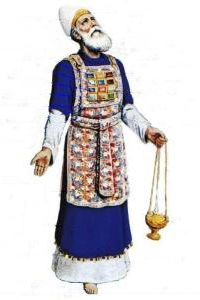
\includegraphics[width=50mm,scale=1.5]{Extras/Melchisedec.jpg}
\vspace{0.4in}  % Create a title for the document and write it in bold font
\LARGE{\textbf{\date}} % Again, do a line break
\linebreak 
% Create a subtitle \large{with Outlines, Statistics, Cross References, and Notes}
\vspace{0.5in}
\begin{flushleft}
\LARGE{Day \#45: Monday, 14 February 2022  \\}\vspace{0.25in}
\LARGE{Numbers 13-15 Psalm 45 Proverb 14}
\end{flushleft}
\vspace{0.6in}
\bigskip

\normalsize{Xenia, Oh.\\}
\normalsize{created: \today}
\vspace{1.3in}

\end{flushright}
\end{titlepage}

\newpage 
\tableofcontents\hypertarget{TOC}{}
\listoffigures
\listoftables

\hyphenation{A-bim-e-lech bre-thren E-phra-im  Gib-e-o-nites Jer-u-sa-lem through-out Phil-i-stines The-o-phil-us Am-a-le-kites ven-geance Mesh-el-e-mi-ah onan-ism Phar-a-oh thoughts grev-ous-ness Hach-a-liah adul-ter-er Shad-rach}

%%%%%%%%%%%%%%%%% EXTRA COLORS
%%%%%%%%%%%%%%%%% EXTRA COLORS
%%%%%%%%%%%%%%%%% EXTRA COLORS
\definecolor{champagne}{rgb}{0.97,0.91,0.81}
\definecolor{bone}{rgb}{0.89,0.85,0.79}

\definecolor{ForestGreen}{rgb}{0.00,0.29,0.098}
\definecolor{GIVING}{cmyk}{1,0.0,0.72,.1}

\definecolor{MLPE}{cmyk}{1,1,0,.45}
\definecolor{SOCCER}{cmyk}{.77, 0, .42, .49}
\definecolor{PAYBILL}{cmyk}{0,0.83,0.76,0.07}
\definecolor{SERMON}{cmyk}{.14,.9,0,.30} % aka seance \href{http://www.flatuicolorpicker.com/purple-cmyk-color-model/}{seance}
\definecolor{BIBLE}{cmyk}{0,.17,.74,.17}
\definecolor{WORKBLUE}{cmyk}{1, .5, 0, .6}
\definecolor{myOrange}{cmyk}{0, .4, .98, .03}
\definecolor{myTan}{cmyk}{0.0,.07,.17,.10}
\definecolor{myRed}{cmyk}{0,1,1,0}
\definecolor{myWhite}{cmyk}{0,0,0,0}
\definecolor{BLUESoD}{cmyk}{.97,.84,0,.04}
\definecolor{WHITE}{cmyk}{0,0,0,0}
\definecolor{OLDGOLD}{cmyk}{0.05,0.3,1.00,0}
\definecolor{CASTLETON}{cmyk}{1,0,0.31,0.66}
\definecolor{cadmiumgreen}{rgb}{0.0, 0.42, 0.24}
\definecolor{jungle}{rgb}{0.203,0.4882,0.1718}
\definecolor{MYGOLD}{rgb}{1,.84,0}

\definecolor{MYLIGHTGRAY}{rgb}{.85,.85,.85}

\definecolor{codegreen}{rgb}{0,0.6,0}
\definecolor{codegray}{rgb}{0.5,0.5,0.5}
\definecolor{codepurple}{rgb}{0.58,0,0.82}
\definecolor{backcolour}{rgb}{0.95,0.95,0.92}


\mdfdefinestyle{MyFrame}{%
    linecolor=blue,
    outerlinewidth=2pt,
    roundcorner=5pt,
    innertopmargin=\baselineskip,
    innerbottommargin=\baselineskip,
    innerrightmargin=10pt,
    innerleftmargin=10pt,
    backgroundcolor=gray!25!white}


\mdfdefinestyle{MyFrame2}{%
    linecolor=black,
    outerlinewidth=2pt,
    roundcorner=5pt,
    innertopmargin=\baselineskip,
    innerbottommargin=\baselineskip,
    innerrightmargin=10pt,
    innerleftmargin=10pt,
    backgroundcolor=yellow!25!white}


%%%%%
%% for PFTTIS list
%%%%%

%%% And Joseph said unto
\index[PFTTIS]{And Joseph said unto!Genesis!Gen 40:008}
\index[PFTTIS]{And Joseph said unto!Genesis!Gen 40:012}
\index[PFTTIS]{And Joseph said unto!Genesis!Gen 41:025}
\index[PFTTIS]{And Joseph said unto!Genesis!Gen 42:014}
\index[PFTTIS]{And Joseph said unto!Genesis!Gen 42:018}
\index[PFTTIS]{And Joseph said unto!Genesis!Gen 44:015}
\index[PFTTIS]{And Joseph said unto!Genesis!Gen 45:003}
\index[PFTTIS]{And Joseph said unto!Genesis!Gen 45:004}
\index[PFTTIS]{And Joseph said unto!Genesis!Gen 46:031}
\index[PFTTIS]{And Joseph said unto!Genesis!Gen 48:009}
\index[PFTTIS]{And Joseph said unto!Genesis!Gen 48:018}
\index[PFTTIS]{And Joseph said unto!Genesis!Gen 50:019}
\index[PFTTIS]{And Joseph said unto!Genesis!Gen 50:024}


%%% a shadow
\index[PFTTIS]{a shadow!1Chronicles!1Chr 029:15}
\index[PFTTIS]{a shadow!Job!Job 008:09}
\index[PFTTIS]{a shadow!Job!Job 014:02}
\index[PFTTIS]{a shadow!Job!Job 017:07}
\index[PFTTIS]{a shadow!Psalm!Psa 102:011}
\index[PFTTIS]{a shadow!Psalm!Psa 144:004}
\index[PFTTIS]{a shadow!Ecclesiastes!Eccl 006:012}
\index[PFTTIS]{a shadow!Ecclesiastes!Eccl 008:013}
\index[PFTTIS]{a shadow!Isaiah!Isa 04:006}
\index[PFTTIS]{a shadow!Isaiah!Isa 25:004}
\index[PFTTIS]{a shadow!Jonah!Jnh 04:06}
\index[PFTTIS]{a shadow!Colossians!Col 02:017}
\index[PFTTIS]{a shadow!Hebews!Heb 10:001}

%%% blessed is the man
\index[PFTTIS]{blessed is the man!Psalm!Psa 001:001}
\index[PFTTIS]{blessed is the man!Psalm!Psa 032:002}
\index[PFTTIS]{blessed is the man!Psalm!Psa 034:008}
\index[PFTTIS]{blessed is the man!Psalm!Psa 065:004}
\index[PFTTIS]{blessed is the man!Psalm!Psa 084:005}
\index[PFTTIS]{blessed is the man!Psalm!Psa 084:012}
\index[PFTTIS]{blessed is the man!Psalm!Psa 094:012}
\index[PFTTIS]{blessed is the man!Psalm!Psa 112:001}
\index[PFTTIS]{blessed is the man!Proverbs!Pro 008:034}
\index[PFTTIS]{blessed is the man!Isaiah!Isa 056:002}
\index[PFTTIS]{blessed is the man!Jeremiah!Jer 017:007}
\index[PFTTIS]{blessed is the man!Romans!Rom 004:008}
\index[PFTTIS]{blessed is the man!James!Jam 001:012}


%%% carry them
\index[PFTTIS]{carry them!Leviticus!Lev 14:045}
\index[PFTTIS]{carry them!Numbers!Num 11:012}
\index[PFTTIS]{carry them!Joshua!Jsh 04:003}
\index[PFTTIS]{carry them!1Samuel!1Sam 20:040}
\index[PFTTIS]{carry them!1Kings!1Kng 08:046}
\index[PFTTIS]{carry them!2Chronicles!2Chr 06:036}
\index[PFTTIS]{carry them!Ezra!Ezra 05:015}
\index[PFTTIS]{carry them!Isaiah!Isa 40:011}
\index[PFTTIS]{carry them!Isaiah!Isa 41:016}
\index[PFTTIS]{carry them!Isaiah!Isa 57:013}
\index[PFTTIS]{carry them!Jeremiah!Jer 20:004}
\index[PFTTIS]{carry them!Jeremiah!Jer 20:005}
\index[PFTTIS]{carry them!Jeremiah!Jer 43:012}


\index[PFTTIS]{good tidings!2Samuel!2Sam 18:027}
\index[PFTTIS]{good tidings!1Kings!1Ki 01:042}
\index[PFTTIS]{good tidings!2Kings!2Ki 07:009 (2x)}
\index[PFTTIS]{good tidings!Isaiah!Isa 40:009 (2x)}
\index[PFTTIS]{good tidings!Isaiah!Isa 41:007}
\index[PFTTIS]{good tidings!Isaiah!Isa 52:007}
\index[PFTTIS]{good tidings!Isaiah!Isa 61:001}
\index[PFTTIS]{good tidings!Nahum!Nah 01:005}
\index[PFTTIS]{good tidings!Luke!Lk 02:010}
\index[PFTTIS]{good tidings!1Thessalonians!1Thess 03:006}


%%% dead body
\index[PFTTIS]{dead body!Leviticus!Lev 21:011}
\index[PFTTIS]{dead body!Numbers!Num 06:006}
\index[PFTTIS]{dead body!Numbers!Num 09:006}
\index[PFTTIS]{dead body!Numbers!Num 09:007}
\index[PFTTIS]{dead body!Numbers!Num 09:010}
\index[PFTTIS]{dead body!Numbers!Num 09:011}
\index[PFTTIS]{dead body!Numbers!Num 09:013}
\index[PFTTIS]{dead body!Numbers!Num 09:016}
\index[PFTTIS]{dead body!2Kings!2Ki 08:005}
\index[PFTTIS]{dead body!Isaiah!Isa 26:019}
\index[PFTTIS]{dead body!Jeremiah!Jer 26:023}
\index[PFTTIS]{dead body!Jeremiah!Jer 36:030}
\index[PFTTIS]{dead body!Haggai!Hag 02:013}

%%% great sea
\index[PFTTIS]{great sea!Numbers!Num 34:006}
\index[PFTTIS]{great sea!Numbers!Num 34:007}
\index[PFTTIS]{great sea!Joshua!Jos 01:004}
\index[PFTTIS]{great sea!Joshua!Jos 09:001}
\index[PFTTIS]{great sea!Joshua!Jos 15:012}
\index[PFTTIS]{great sea!Joshua!Jos 15:047}
\index[PFTTIS]{great sea!Joshua!Jos 23:004}
\index[PFTTIS]{great sea!Ezekiel!Eze 47:010}
\index[PFTTIS]{great sea!Ezekiel!Eze 47:015}
\index[PFTTIS]{great sea!Ezekiel!Eze 47:019}
\index[PFTTIS]{great sea!Ezekiel!Eze 47:020}
\index[PFTTIS]{great sea!Ezekiel!Eze 48:028}
\index[PFTTIS]{great sea!Daniel!Dan 07:002}


%%% have forsaken me
\index[PFTTIS]{have forsaken me!Judges!Jdg 10:013}
\index[PFTTIS]{have forsaken me!1Samuel!1Sam 08:008}
\index[PFTTIS]{have forsaken me!1Kings!1Ki 11:033}
\index[PFTTIS]{have forsaken me!2Kings!2Ki 22:017}
\index[PFTTIS]{have forsaken me!2Chronicles!2Chr 12:005}
\index[PFTTIS]{have forsaken me!2Chronicles!2Chr 34:025}
\index[PFTTIS]{have forsaken me!Jeremiah!Jer 01:016}
\index[PFTTIS]{have forsaken me!Jeremiah!Jer 02:013}
\index[PFTTIS]{have forsaken me!Jeremiah!Jer 05:007}
\index[PFTTIS]{have forsaken me!Jeremiah!Jer 05:019}
\index[PFTTIS]{have forsaken me!Jeremiah!Jer 16:011 (2x)}
\index[PFTTIS]{have forsaken me!Jeremiah!Jer 19:004}

%%% no king
\index[PFTTIS]{no king!Judges!Jdg 17:06}
\index[PFTTIS]{no king!Judges!Jdg 18:01}
\index[PFTTIS]{no king!Judges!Jdg 19:01}
\index[PFTTIS]{no king!Judges!Jdg 21:25}
\index[PFTTIS]{no king!1Kings!1Ki 22:47}
\index[PFTTIS]{no king!2Kings!2Ki 23:25}
\index[PFTTIS]{no king!Nehemiah!Neh 13:26}
\index[PFTTIS]{no king!Psalms!Psa 033:016}
\index[PFTTIS]{no king!Proverbs!Pro 30:27}
\index[PFTTIS]{no king!Daniel!Dan 02:10}
\index[PFTTIS]{no king!Hosea!Hos 10:03}
\index[PFTTIS]{no king!Micah!Mic 04:09}
\index[PFTTIS]{no king!John!Jhn 19:15}


%%% rebellious house
\index[PFTTIS]{rebellious house!Exodus!Exo 02:005}
\index[PFTTIS]{rebellious house!Exodus!Exo 02:006}
\index[PFTTIS]{rebellious house!Exodus!Exo 02:008}
\index[PFTTIS]{rebellious house!Exodus!Exo 03:009}
\index[PFTTIS]{rebellious house!Exodus!Exo 03:026}
\index[PFTTIS]{rebellious house!Exodus!Exo 03:027}
\index[PFTTIS]{rebellious house!Exodus!Exo 12:002 (2x)}
\index[PFTTIS]{rebellious house!Exodus!Exo 12:003}
\index[PFTTIS]{rebellious house!Exodus!Exo 12:009}
\index[PFTTIS]{rebellious house!Exodus!Exo 12:025}
\index[PFTTIS]{rebellious house!Exodus!Exo 17:012}
\index[PFTTIS]{rebellious house!Exodus!Exo 24:003}

%%% seek him
\index[PFTTIS]{seek him!Deuteronomy!Deu 04:029}\index[PFTTIS]{seek him!1Samuel!1Sam 23:025}
\index[PFTTIS]{seek him!1Chronicles!1Chr 28:009}
\index[PFTTIS]{seek him!2Chronicles!1Chr 15:002}
\index[PFTTIS]{seek him!Ezra!Ezr 08:022}
\index[PFTTIS]{seek him!Psalms!Psa 022:026}
\index[PFTTIS]{seek him!Psalms!Psa 024:006}
\index[PFTTIS]{seek him!Psalms!Psa 119:002}
\index[PFTTIS]{seek him!SoS!SoS 03:002}
\index[PFTTIS]{seek him!SoS!SoS 06:001}
\index[PFTTIS]{seek him!Hosea!Hos 07:010}
\index[PFTTIS]{seek him!Amos!Amo 05:008}
\index[PFTTIS]{seek him!Hebrews!Heb 11:0063}


%%% seek ye
\index[PFTTIS]{seek ye!Isaiah!Isa 34:016}
\index[PFTTIS]{seek ye!Isaiah!Isa 45:019}
\index[PFTTIS]{seek ye!Isaiah!Isa 55:006}
\index[PFTTIS]{seek ye!Amos!Amos 5:004}
\index[PFTTIS]{seek ye!John!John 1:38}
\index[PFTTIS]{seek ye!John!John 18:4}
\index[PFTTIS]{seek ye!John!John 18:7}
\index[PFTTIS]{seek ye!Matthew!Matt 6:33}
\index[PFTTIS]{seek ye!Numbers!Num 16:10}
\index[PFTTIS]{seek ye!Luke!Luke 12:31}
\index[PFTTIS]{seek ye!Luke!Luke 24:5}
\index[PFTTIS]{seek ye!Psalm!Psa 27:8}
\index[PFTTIS]{seek ye!Zephaniah!Zeph 2:3}

%%% the uncircumcised
\index[PFTTIS]{the uncircumcised!Genesis!Gen 17:014}
\index[PFTTIS]{the uncircumcised!Judges!Jdg 14:003}
\index[PFTTIS]{the uncircumcised!Judges!Jdg 15:018}
\index[PFTTIS]{the uncircumcised!2Samuel!2Sam 01:020}
\index[PFTTIS]{the uncircumcised!Isaiah!Isa 02:001}
\index[PFTTIS]{the uncircumcised!Jeremiah!Jer 09:025}
\index[PFTTIS]{the uncircumcised!Ezekiel!Eze 28:010}
\index[PFTTIS]{the uncircumcised!Ezekiel!Eze 31:018}
\index[PFTTIS]{the uncircumcised!Ezekiel!Eze 32:019}
\index[PFTTIS]{the uncircumcised!Ezekiel!Eze 32:027}
\index[PFTTIS]{the uncircumcised!Ezekiel!Eze 32:028}
\index[PFTTIS]{the uncircumcised!Ezekiel!Eze 32:029}
\index[PFTTIS]{the uncircumcised!Ezekiel!Eze 32:032}

%%% worship him
\index[PFTTIS]{worship him!Psalms!Psa 97:007}
\index[PFTTIS]{worship him!Zephaniah!Zeph 02:011}
\index[PFTTIS]{worship him!Matthew!Matt 02:002}
\index[PFTTIS]{worship him!Matthew!Matt 02:008}
\index[PFTTIS]{worship him!John!John 04:023}
\index[PFTTIS]{worship him!John!John 04:024 (2x)} 
\index[PFTTIS]{worship him!Acts!Acts 17:023}
\index[PFTTIS]{worship him!Hebrews!Heb 01:006}
\index[PFTTIS]{worship him!Revelation!Rev 04:010}
\index[PFTTIS]{worship him!Revelation!Rev 13:008}
\index[PFTTIS]{worship him!Revelation!Rev 14:007}
\index[PFTTIS]{worship him!Revelation!Rev 19:010}


%%%%%
%% for PFTTIS list
%%%%%

%%% afflictions
\index[WFTTIS]{afflictions!Psalms!Psa 34:019}
\index[WFTTIS]{afflictions!Psalms!Psa 132:001}
\index[WFTTIS]{afflictions!Acts!Acts 07:010}
\index[WFTTIS]{afflictions!Acts!Acts 20:023}
\index[WFTTIS]{afflictions!2Corinthians!2Cor 06:004}
\index[WFTTIS]{afflictions!Colossians!Col 01:024}
\index[WFTTIS]{afflictions!1Thessalonians!1Thess 03:003}
\index[WFTTIS]{afflictions!2Timothy!2Tim 01:008}
\index[WFTTIS]{afflictions!2Timothy!2Tim 03:011}
\index[WFTTIS]{afflictions!2Timothy!2Tim 04:005}
\index[WFTTIS]{afflictions!Hebrews!Heb 10:032}
\index[WFTTIS]{afflictions!Hebrews!Heb 10:033}
\index[WFTTIS]{afflictions!1Peter!1Pet 05:009}

%%% acsend
\index[WFTTIS]{acsend!Joshua!Jos 06:05}
\index[WFTTIS]{acsend!Psalm!Psa 024:003}
\index[WFTTIS]{acsend!Psalm!Psa 135:007}
\index[WFTTIS]{acsend!Psalm!Psa 139:008}
\index[WFTTIS]{acsend!Isaiah!Isa 14:013}
\index[WFTTIS]{acsend!Isaiah!Isa 14:014}
\index[WFTTIS]{acsend!Jeremiah!Jer 10:013}
\index[WFTTIS]{acsend!Jeremiah!Jer 51:016}
\index[WFTTIS]{acsend!Ezekiel!Eze 38:009}
\index[WFTTIS]{acsend!John!John 06:062}
\index[WFTTIS]{acsend!John!John 20:017}
\index[WFTTIS]{acsend!Romans!Rom 10:006}
\index[WFTTIS]{acsend!Revelation!Rev 17:008}

%%% Assyrian
\index[WFTTIS]{Assyrian!Isaiah!Isa 10:005}
\index[WFTTIS]{Assyrian!Isaiah!Isa 10:024}
\index[WFTTIS]{Assyrian!Isaiah!Isa 14:025}
\index[WFTTIS]{Assyrian!Isaiah!Isa 19:023}
\index[WFTTIS]{Assyrian!Isaiah!Isa 23:013}
\index[WFTTIS]{Assyrian!Isaiah!Isa 30:031}
\index[WFTTIS]{Assyrian!Isaiah!Isa 31:008}
\index[WFTTIS]{Assyrian!Isaiah!Isa 52:004}
\index[WFTTIS]{Assyrian!Ezekiel!Eze 31:003}
\index[WFTTIS]{Assyrian!Hosea!Hos 05:013}
\index[WFTTIS]{Assyrian!Hosea!Hos 11:005}
\index[WFTTIS]{Assyrian!Micah!Hos 05:005}
\index[WFTTIS]{Assyrian!Micah!Hos 05:006}

%%% blot
\index[WFTTIS]{blot!Exodus!Exo 32:032}
\index[WFTTIS]{blot!Exodus!Exo 32:033}
\index[WFTTIS]{blot!Numbers!Num 05:026}
\index[WFTTIS]{blot!Deuteronomy!Deut 09:014}
\index[WFTTIS]{blot!Deuteronomy!Deut 25:019}
\index[WFTTIS]{blot!Deuteronomy!Deut 29:020}
\index[WFTTIS]{blot!2Kings!2Ki 14:027}
\index[WFTTIS]{blot!Job!Job 31:007}
\index[WFTTIS]{blot!Psalms!Psa 51:001}
\index[WFTTIS]{blot!Psalms!Psa 51:009}
\index[WFTTIS]{blot!Proverbs!Pro 09:007}
\index[WFTTIS]{blot!Jeremiah!Jer 18:023}
\index[WFTTIS]{blot!Revelation!Rev 03:005}


%%% chain
\index[WFTTIS]{chain!Genesis!Gen 41:042}
\index[WFTTIS]{chain!1Kings!1Ki 07:017}
\index[WFTTIS]{chain!Psalms!Psa 73:006}
\index[WFTTIS]{chain!SoS!Sos 04:009}
\index[WFTTIS]{chain!Lamentations!Lam 03:007}
\index[WFTTIS]{chain!Ezekiel!Eze 07:023}
\index[WFTTIS]{chain!Ezekiel!Eze 16:011}
\index[WFTTIS]{chain!Daniel!Dan 05:007}
\index[WFTTIS]{chain!Daniel!Dan 05:016}
\index[WFTTIS]{chain!Daniel!Dan 05:029}
\index[WFTTIS]{chain!Acts!Acts 28:020}
\index[WFTTIS]{chain!2Timothy!2Tim 01:016}
\index[WFTTIS]{chain!Revelation!Rev 20:001}


%%% controversy
\index[WFTTIS]{controversy!Deuteronomy!Deu 17:008}
\index[WFTTIS]{controversy!Deuteronomy!Deu 19:017}
\index[WFTTIS]{controversy!Deuteronomy!Deu 21:005}
\index[WFTTIS]{controversy!Deuteronomy!Deu 25:001}
\index[WFTTIS]{controversy!2Samuel!2Sam 15:002}
\index[WFTTIS]{controversy!Isaiah!Isa 34:008}
\index[WFTTIS]{controversy!Jeremiah!Jer 25:031}
\index[WFTTIS]{controversy!Ezekiel!Eze 44:024}
\index[WFTTIS]{controversy!Hosea!Hos 04:001}
\index[WFTTIS]{controversy!Hosea!Hos 12:002}
\index[WFTTIS]{controversy!Micah!Mic 06:002 (2x)}
\index[WFTTIS]{controversy!1Timothy!1Tim 03:016}


%%% Dagon/Dagon's
\index[WFTTIS]{Dagon!Judges!Jdg 16:023}
\index[WFTTIS]{Dagon!1Samuel!1Sam 05:002 (2x)}
\index[WFTTIS]{Dagon!1Samuel!1Sam 05:003 (2x)}
\index[WFTTIS]{Dagon!1Samuel!1Sam 05:004 (3x)}
\index[WFTTIS]{Dagon!1Samuel!1Sam 05:005 (3x)}
\index[WFTTIS]{Dagon!1Samuel!1Sam 05:007}
\index[WFTTIS]{Dagon!1Chronicles!1Chr 10:010}

%%% disobedient
\index[WFTTIS]{disobedient!1Kings!1Ki 13:026}
\index[WFTTIS]{disobedient!Nehemiah!Neh 09:026}
\index[WFTTIS]{disobedient!Luke!Luke 01:017}
\index[WFTTIS]{disobedient!Acts!Acts 26:019}
\index[WFTTIS]{disobedient!Romans!Rom 01:030}
\index[WFTTIS]{disobedient!Romans!Rom 10:021}
\index[WFTTIS]{disobedient!1Timothy!1Tim 01:009}
\index[WFTTIS]{disobedient!2Timothy!2Tim 03:002}
\index[WFTTIS]{disobedient!Titus!Titus 01:016}
\index[WFTTIS]{disobedient!Titus!Titus 03:003}
\index[WFTTIS]{disobedient!1Peter!1Pet 02:007}
\index[WFTTIS]{disobedient!1Peter!1Pet 02:008}
\index[WFTTIS]{disobedient!1Peter!1Pet 03:020}


%%% doubt
\index[WFTTIS]{doubt!Genesis!Gen 37:033}
\index[WFTTIS]{doubt!Deuteronomy!Deu 28:066}
\index[WFTTIS]{doubt!Job!Job 12:002}
\index[WFTTIS]{doubt!Matthew!Matt 14:031}
\index[WFTTIS]{doubt!Matthew!Matt 21:021}
\index[WFTTIS]{doubt!Mark!Mk 11:023}
\index[WFTTIS]{doubt!Luke!Lk 11:020}
\index[WFTTIS]{doubt!John!Jhn 10:024}
\index[WFTTIS]{doubt!Acts!Acts 02:012}
\index[WFTTIS]{doubt!Acts!Acts 28:004}
\index[WFTTIS]{doubt!1Corinthians!1Cor 09:010}
\index[WFTTIS]{doubt!Galatians!Gal 04:020}
\index[WFTTIS]{doubt!1John!1Jhn 02:019}


%%% dungeon
\index[WFTTIS]{dungeon!Genesis!Gen 40:015}
\index[WFTTIS]{dungeon!Genesis!Gen 41:014}
\index[WFTTIS]{dungeon!Exodus!Exo 12:029}
\index[WFTTIS]{dungeon!Jeremiah!Jer 37:016}
\index[WFTTIS]{dungeon!Jeremiah!Jer 38:006 (2x)}
\index[WFTTIS]{dungeon!Jeremiah!Jer 38:007}
\index[WFTTIS]{dungeon!Jeremiah!Jer 38:009}
\index[WFTTIS]{dungeon!Jeremiah!Jer 38:010}
\index[WFTTIS]{dungeon!Jeremiah!Jer 38:011}
\index[WFTTIS]{dungeon!Jeremiah!Jer 38:013}
\index[WFTTIS]{dungeon!Lamentations!Lam 03:053}
\index[WFTTIS]{dungeon!Lamentations!Lam 03:055}


%%% error
\index[WFTTIS]{error!2Samuel!2Sam 06:007}
\index[WFTTIS]{error!Job!Job 19:004}
\index[WFTTIS]{error!Ecclesiastes!Ecc 05:006}
\index[WFTTIS]{error!Ecclesiastes!Ecc 10:005}
\index[WFTTIS]{error!Isaiah!Isa 32:006}
\index[WFTTIS]{error!Daniel!Dan 06:004}
\index[WFTTIS]{error!Matthew!Matt 27:064}
\index[WFTTIS]{error!Romans!Rom 01:027}
\index[WFTTIS]{error!James!Jam 05:020}
\index[WFTTIS]{error!2Peter!2Pet 02:018}
\index[WFTTIS]{error!2Peter!2Pet 03:017}
\index[WFTTIS]{error!1John!1Jn 04:006}
\index[WFTTIS]{error!Jude!Jude 01:011}

%%% fourish
\index[WFTTIS]{fourish!Psalms!Psa 072:007}
\index[WFTTIS]{fourish!Psalms!Psa 072:016}
\index[WFTTIS]{fourish!Psalms!Psa 092:007}
\index[WFTTIS]{fourish!Psalms!Psa 092:012}
\index[WFTTIS]{fourish!Psalms!Psa 092:013}
\index[WFTTIS]{fourish!Psalms!Psa 132:018}
\index[WFTTIS]{fourish!Proverbs!Pro 11:28}
\index[WFTTIS]{fourish!Proverbs!Pro 14:11}
\index[WFTTIS]{fourish!Ecclesiastes!Ecc 12:05}
\index[WFTTIS]{fourish!SongOfSolomon!SOS 07:12}
\index[WFTTIS]{fourish!Isaiah!Isa 17:11}
\index[WFTTIS]{fourish!Isaiah!Isa 66:14}
\index[WFTTIS]{fourish!Ezekiel!Eze 17:24}




%%% giants
\index[WFTTIS]{giants!Genesis!Gen 06:004}
\index[WFTTIS]{giants!Numbers!Num 13:033}
\index[WFTTIS]{giants!Deuteronomy!Deut 02:011}
\index[WFTTIS]{giants!Deuteronomy!Deut 02:021}
\index[WFTTIS]{giants!Deuteronomy!Deut 03:011}
\index[WFTTIS]{giants!Deuteronomy!Deut 03:013}
\index[WFTTIS]{giants!Joshua!Josh 12:004}
\index[WFTTIS]{giants!Joshua!Josh 13:012}
\index[WFTTIS]{giants!Joshua!Josh 15:008}
\index[WFTTIS]{giants!Joshua!Josh 17:015}
\index[WFTTIS]{giants!Joshua!Josh 16:016}

%%% good man
\index[WFTTIS]{good man!2 Samuel!2Sa 18:27}
%(1) Psalms 37:23 [5]
%(1) Psalms 112:5 [2]
%(1) Proverbs 12:2 [2]
%(1) Proverbs 13:22 [2]
%(1) Proverbs 14:14 [14]
%(1) Micah 7:2 [2]
%(1) Matthew 12:35 [2]
%(1) Luke 6:45 [2]
%(1) Luke 23:50 [15]
%(1) John 7:12 [17]
%(1) Acts 11:24 [5]
%(1) Romans 5:7 [14]

%%% Hinnom
\index[WFTTIS]{Hinnom!Joshua!Jsh 15:008}
\index[WFTTIS]{Hinnom!Joshua!Jsh 18:016}
\index[WFTTIS]{Hinnom!2Kings!2Ki 23:010}
\index[WFTTIS]{Hinnom!2Chronicles!2Chr 28:003}
\index[WFTTIS]{Hinnom!2Chronicles!2Chr 33:006}
\index[WFTTIS]{Hinnom!Nehemiah!Neh 11:030}
\index[WFTTIS]{Hinnom!Jeremiah!Jer 07:031}
\index[WFTTIS]{Hinnom!Jeremiah!Jer 07:032}
\index[WFTTIS]{Hinnom!Jeremiah!Jer 19:002}
\index[WFTTIS]{Hinnom!Jeremiah!Jer 19:006}
\index[WFTTIS]{Hinnom!Jeremiah!Jer 32:035}

%%% inclined
\index[WFTTIS]{inclined!Judges!Jdg 09:003}
\index[WFTTIS]{inclined!Psalms!Psa 040:001}
\index[WFTTIS]{inclined!Psalms!Psa 116:002}
\index[WFTTIS]{inclined!Psalms!Psa 119:112}
\index[WFTTIS]{inclined!Proverbs!Pro 05:13}
\index[WFTTIS]{inclined!Jeremiah!Jer 07:24}
\index[WFTTIS]{inclined!Jeremiah!Jer 07:26}
\index[WFTTIS]{inclined!Jeremiah!Jer 11:08}
\index[WFTTIS]{inclined!Jeremiah!Jer 17:23}
\index[WFTTIS]{inclined!Jeremiah!Jer 25:04}
\index[WFTTIS]{inclined!Jeremiah!Jer 34:14}
\index[WFTTIS]{inclined!Jeremiah!Jer 35:15}
\index[WFTTIS]{inclined!Jeremiah!Jer 44:05}


%%% laughed
\index[WFTTIS]{laughed!Genesis!Gen 17:017}
\index[WFTTIS]{laughed!Genesis!Gen 18:012}
\index[WFTTIS]{laughed!Genesis!Gen 18:015}
\index[WFTTIS]{laughed!2Kings!2Ki 19:021}
\index[WFTTIS]{laughed!2Chronicles!2Chr 30:010}
\index[WFTTIS]{laughed!Nehemiah!Neh 02:019}
\index[WFTTIS]{laughed!Job!Job 12:004}
\index[WFTTIS]{laughed!Job!Job 29:024}
\index[WFTTIS]{laughed!Isaiah!Isa 37:022}
\index[WFTTIS]{laughed!Ezekiel!Ezek 23:032}
\index[WFTTIS]{laughed!Matthew!Matt 09:024}
\index[WFTTIS]{laughed!Mark!Mk 05:040}
\index[WFTTIS]{laughed!Luke!Lk 08:053}

%%% liar
\index[WFTTIS]{liar!Job!Job 24:025}
\index[WFTTIS]{liar!Proverbs!Pro 17:004}
\index[WFTTIS]{liar!Proverbs!Pro 19:022}
\index[WFTTIS]{liar!Proverbs!Pro 30:006}
\index[WFTTIS]{liar!Jeremiah!Jer 15:018}
\index[WFTTIS]{liar!John!Jhn 08:044}
\index[WFTTIS]{liar!John!Jhn 08:055}
\index[WFTTIS]{liar!Romans!Rom 03:004}
\index[WFTTIS]{liar!1John!1Jhn 01:010}
\index[WFTTIS]{liar!1John!1Jhn 02:004}
\index[WFTTIS]{liar!1John!1Jhn 02:022}
\index[WFTTIS]{liar!1John!1Jhn 04:020}
\index[WFTTIS]{liar!1John!1Jhn 05:010}

%%% palsy
\index[WFTTIS]{palsy!Matthew!Matt 04:024}
\index[WFTTIS]{palsy!Matthew!Matt 08:006}
\index[WFTTIS]{palsy!Matthew!Matt 09:002}
\index[WFTTIS]{palsy!Matthew!Matt 09:006}
\index[WFTTIS]{palsy!Mark!Mk 02:003}
\index[WFTTIS]{palsy!Mark!Mk 02:004}
\index[WFTTIS]{palsy!Mark!Mk 02:005}
\index[WFTTIS]{palsy!Mark!Mk 02:009}
\index[WFTTIS]{palsy!Mark!Mk 02:010}
\index[WFTTIS]{palsy!Luke!Lk 05:018}
\index[WFTTIS]{palsy!Luke!Lk 05:024}
\index[WFTTIS]{palsy!Acts!Acts 09:033}

%%% Profitable
\index[WFTTIS]{profitable!Job!Job 22:002 (2x)}
\index[WFTTIS]{profitable!Ecclesiastes!Ecc 10:010}
\index[WFTTIS]{profitable!Isaiah!Isa 44:010}
\index[WFTTIS]{profitable!Jeremiah!Jer 13:007}
\index[WFTTIS]{profitable!Matthew!Matt 05:029}
\index[WFTTIS]{profitable!Matthew!Matt 05:030}
\index[WFTTIS]{profitable!Acts!Acts 20:020}
\index[WFTTIS]{profitable!1Timothy!1Tim 04:008}
\index[WFTTIS]{profitable!2Timothy!2Tim 03:016}
\index[WFTTIS]{profitable!2Timothy!2Tim 04:011}
\index[WFTTIS]{profitable!Titus!Titus 03:008}
\index[WFTTIS]{profitable!Philemon!Phlm 01:011}

%%% Rechab
\index[WFTTIS]{Rechab!2Samuel!2Sam 04:002}
\index[WFTTIS]{Rechab!2Samuel!2Sam 04:005}
\index[WFTTIS]{Rechab!2Samuel!2Sam 04:006}
\index[WFTTIS]{Rechab!2Samuel!2Sam 04:009}
\index[WFTTIS]{Rechab!2KIngs!2Ki 10:015}
\index[WFTTIS]{Rechab!2KIngs!2Ki 10:023}
\index[WFTTIS]{Rechab!1Chronicles!1Chr 02:055}
\index[WFTTIS]{Rechab!Nehemiah!Neh 03:014}
\index[WFTTIS]{Rechab!Jeremiah!Jer 35:006}
\index[WFTTIS]{Rechab!Jeremiah!Jer 35:008}
\index[WFTTIS]{Rechab!Jeremiah!Jer 35:014}
\index[WFTTIS]{Rechab!Jeremiah!Jer 35:016}
\index[WFTTIS]{Rechab!Jeremiah!Jer 35:019}

%%% serpents
\index[WFTTIS]{serpents!Exodus!Exo 07:012}
\index[WFTTIS]{serpents!Numbers!Num 21:006}
\index[WFTTIS]{serpents!Numbers!Num 21:007}
\index[WFTTIS]{serpents!Deuteronomy!Deu 08:015}
\index[WFTTIS]{serpents!Deuteronomy!Deu 32:024}
\index[WFTTIS]{serpents!Jeremiah!Jer 08:017}
\index[WFTTIS]{serpents!Matthew!Matt 10:016}
\index[WFTTIS]{serpents!Matthew!Matt 23:033}
\index[WFTTIS]{serpents!Mark!Mk 16:018}
\index[WFTTIS]{serpents!Luke!Lk 10:019}
\index[WFTTIS]{serpents!1Corinthians!1Cor 10:009}
\index[WFTTIS]{serpents!James!Jas 03:007}
\index[WFTTIS]{serpents!Revelation!Rev 09:019}

%%% short
\index[WFTTIS]{short!Numbers!Num 11:023}
\index[WFTTIS]{short!2Kings!2Ki 10:032}
\index[WFTTIS]{short!Job!Job 17:012}
\index[WFTTIS]{short!Job!Job 20:005}
\index[WFTTIS]{short!Psalms!Psa 89:047}
\index[WFTTIS]{short!Romans!Rom 03:023}
\index[WFTTIS]{short!Romans!Rom 09:028  (2x)}
\index[WFTTIS]{short!1Corinthians!1Cor 07:029}
\index[WFTTIS]{short!1Thessalonians!1Thess 02:017}
\index[WFTTIS]{short!Hebrews!Heb 04:001}
\index[WFTTIS]{short!Revelation!Rev 12:012}
\index[WFTTIS]{short!Revelation!Rev 17:010}

%%% smiteth
\index[WFTTIS]{smiteth!Exodus!Exo 21:012}
\index[WFTTIS]{smiteth!Exodus!Exo 21:15}
\index[WFTTIS]{smiteth!Deuteronomy!Dt 25:11}
\index[WFTTIS]{smiteth!Deuteronomy!Dt 27:24}
\index[WFTTIS]{smiteth!Joshua!Jsh 15:16}
\index[WFTTIS]{smiteth!Judges!Jdg 15:16}
\index[WFTTIS]{smiteth!2 Samuel!2Sa 05:08}
\index[WFTTIS]{smiteth!1Chronicles!1Chr 11:06}
\index[WFTTIS]{smiteth!Job!1Chr 26:12}
\index[WFTTIS]{smiteth!Isaiah!Isa 09:13}
\index[WFTTIS]{smiteth!Lamentations!Lam 03:30}
\index[WFTTIS]{smiteth!Ezekiel!Eze 07:09}
\index[WFTTIS]{smiteth!Luke!Lk 06:29}



%%% vanities
\index[WFTTIS]{vanities!Deuteronomy!Deut 21:021}
\index[WFTTIS]{vanities!1Kings!1Ki 16:013}
\index[WFTTIS]{vanities!1Kings!1Ki 16:026}
\index[WFTTIS]{vanities!Psalms!Psa 031:006}
\index[WFTTIS]{vanities!Ecclesiastes!Ecc 01:002 (2x)}
\index[WFTTIS]{vanities!Ecclesiastes!Ecc 05:007}
\index[WFTTIS]{vanities!Ecclesiastes!Ecc 12:008}
\index[WFTTIS]{vanities!Jeremiah!Jer 08:019}
\index[WFTTIS]{vanities!Jeremiah!Jer 10:008}
\index[WFTTIS]{vanities!Jeremiah!Jer 14:022}
\index[WFTTIS]{vanities!Jonah!Jnh 02:008}
\index[WFTTIS]{vanities!Acts!Acts 14:015}



%%%%%
%% for PFTTIS list
%%%%%

%%% worm
\index[WFITV]{worm!Exodus!Exo 16:024}
\index[WFITV]{worm!Job!Job 17:014}
\index[WFITV]{worm!Job!Job 24:029}
\index[WFITV]{worm!Job!Job 25:005 (2x)}
\index[WFITV]{worm!Psalms!Psa 022:006}
\index[WFITV]{worm!Isaiah!Isa 14:011}
\index[WFITV]{worm!Isaiah!Isa 41:014}
\index[WFITV]{worm!Isaiah!Isa 51:008}
\index[WFITV]{worm!Isaiah!Isa 66:024}
\index[WFITV]{worm!Jonah!Jnh 04:007}
\index[WFITV]{worm!Mark!Mk 09:044}
\index[WFITV]{worm!Mark!Mk 09:046}
\index[WFITV]{worm!Mark!Mk 09:048}


%\subsubsection{Title}
%\textbf{Introduction:} Isaiah 46 
%\index[speaker]{Speaker!Isaiah 49 (Title}
%\index[series]{Book (Speaker)!IPassage (Title)}
%\index[date]{2017/07/09!Isaiah 49 (Title)}
%\begin{compactenum}[I.]
%    \item  \textbf{Point} \index[scripture]{Isaiah!IPassage} (IPassage)
%\end{compactenum}




  


%\input{02OT-Exodus/ExodusIntroduction}
\newpage
\begin{figure}
\begin{center}
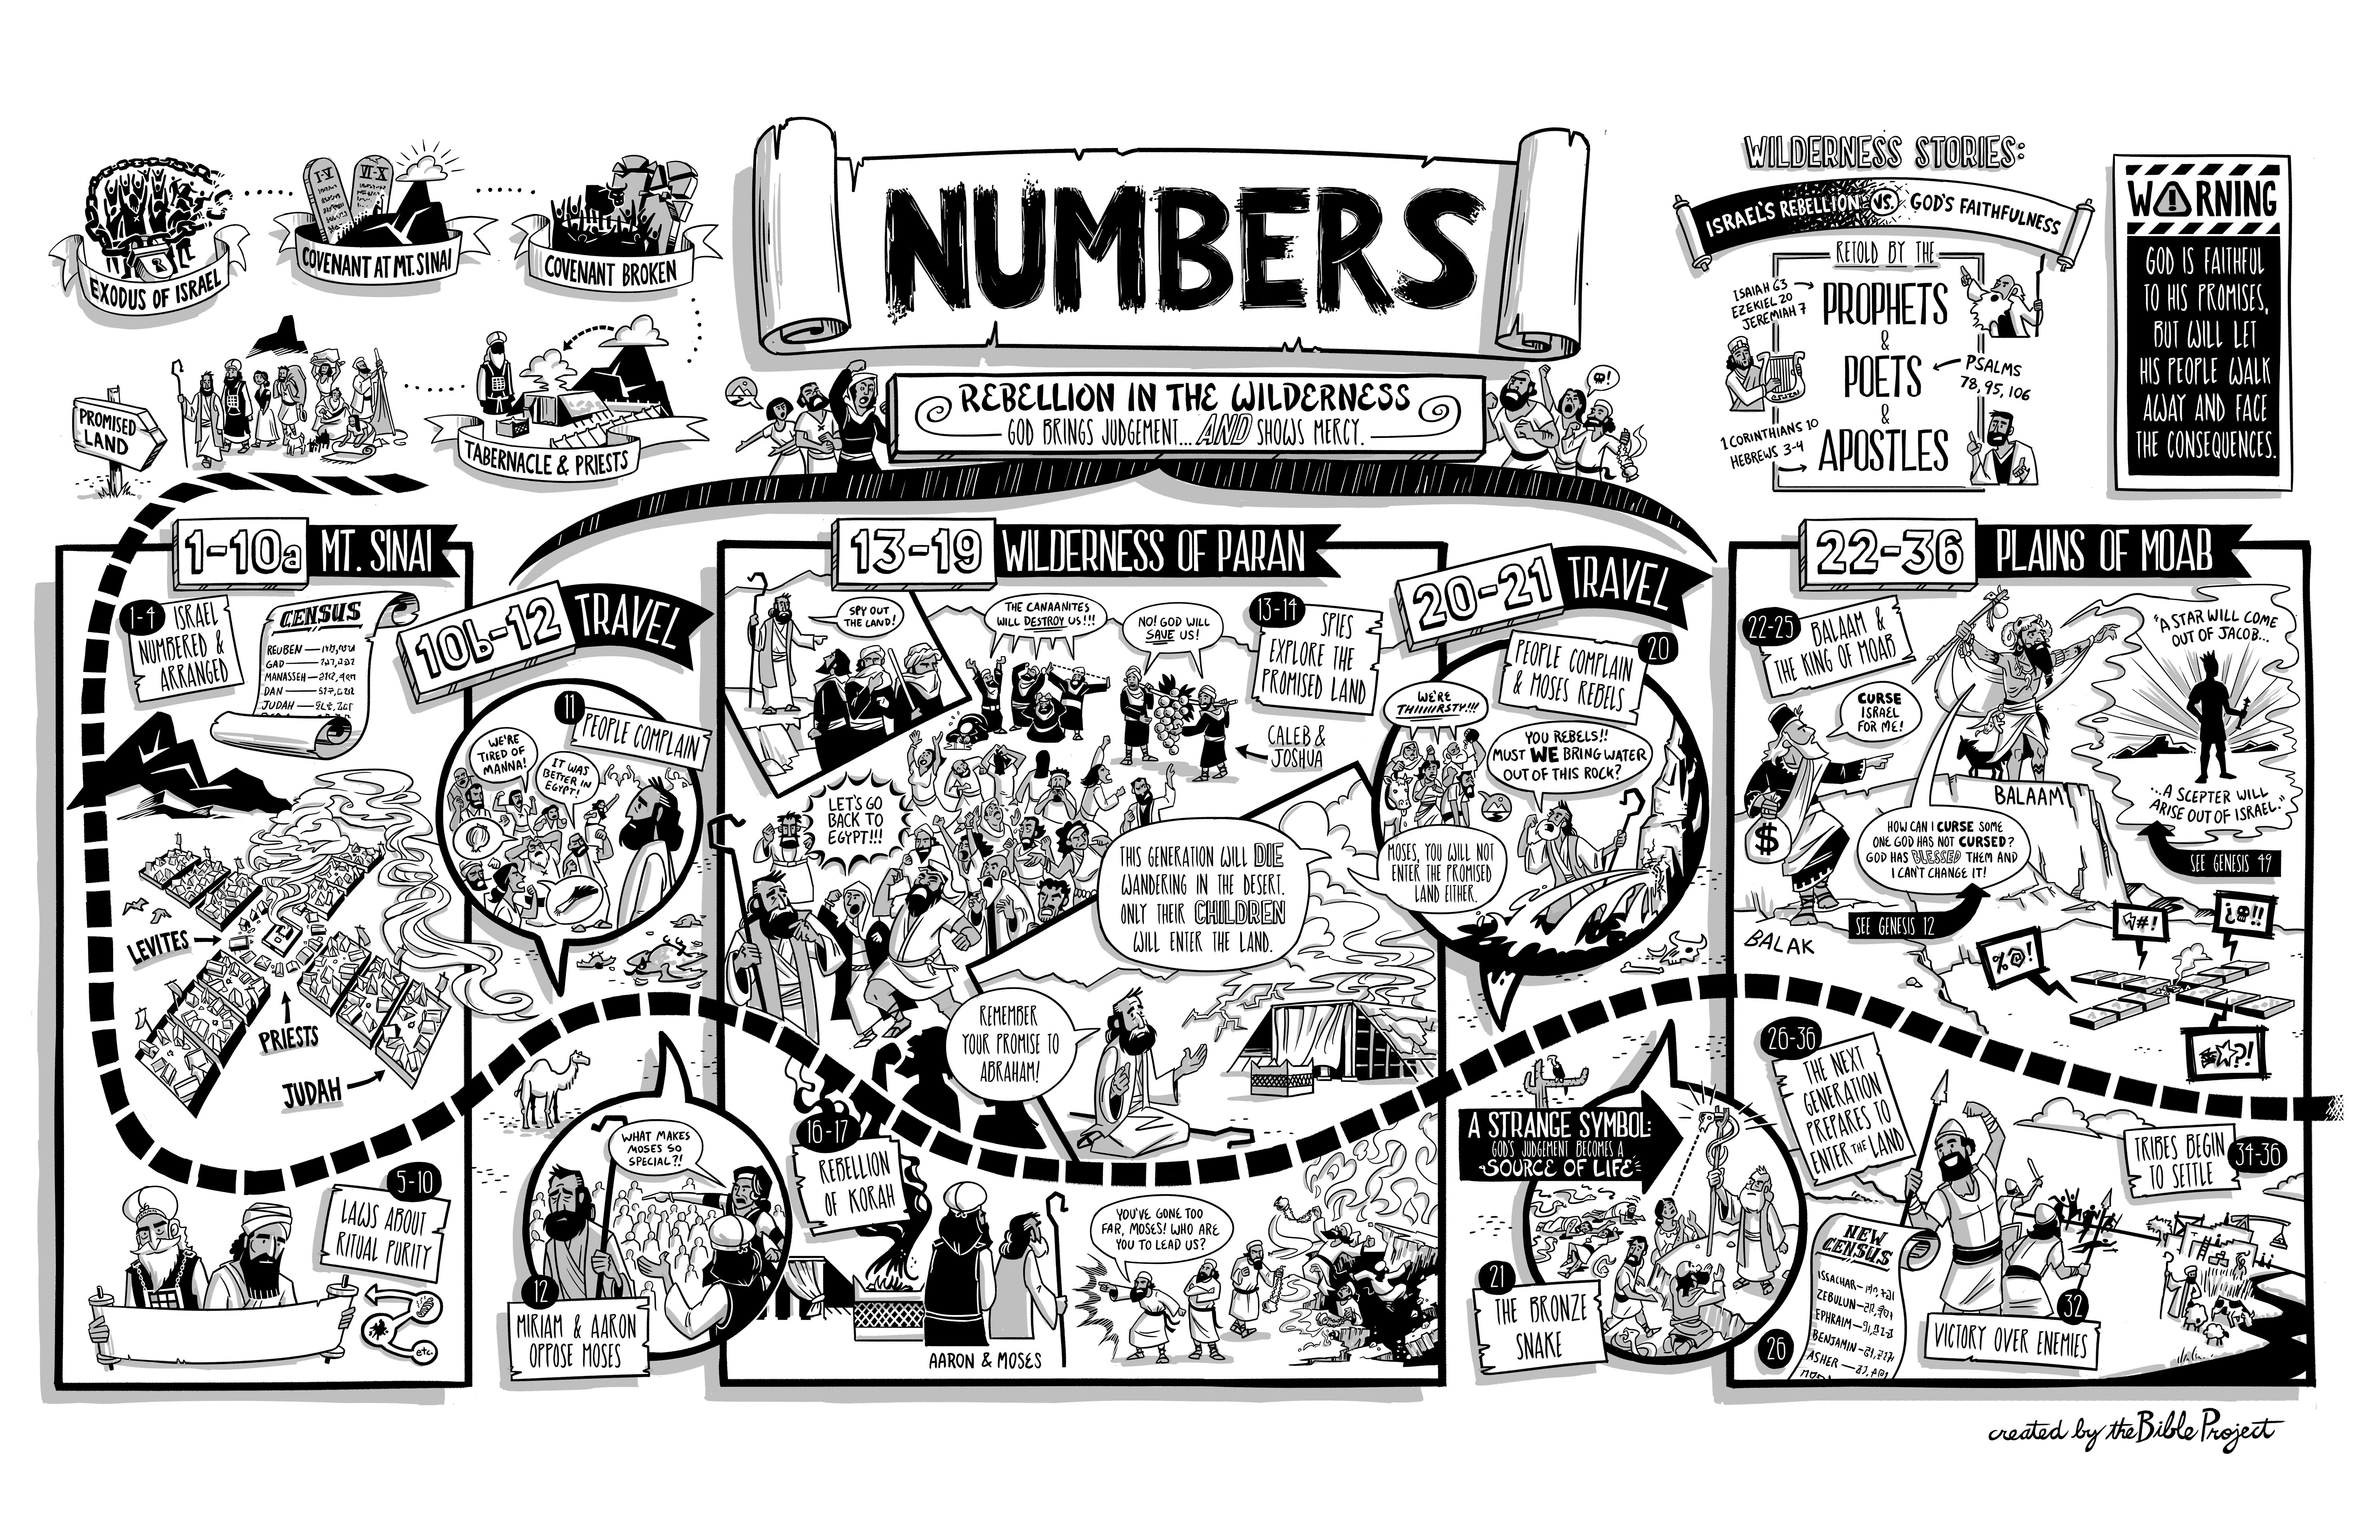
\includegraphics[scale=0.5, angle=90]{04OT-Numbers/References/BibleProject-Numbers.jpg}
\caption[Numbers from the Bible Project]{Numbers from the Bible Project}
\label{fig:Numbers from the Bible Project}
\end{center}
\end{figure}

\newpage
\begin{figure}
\begin{center}
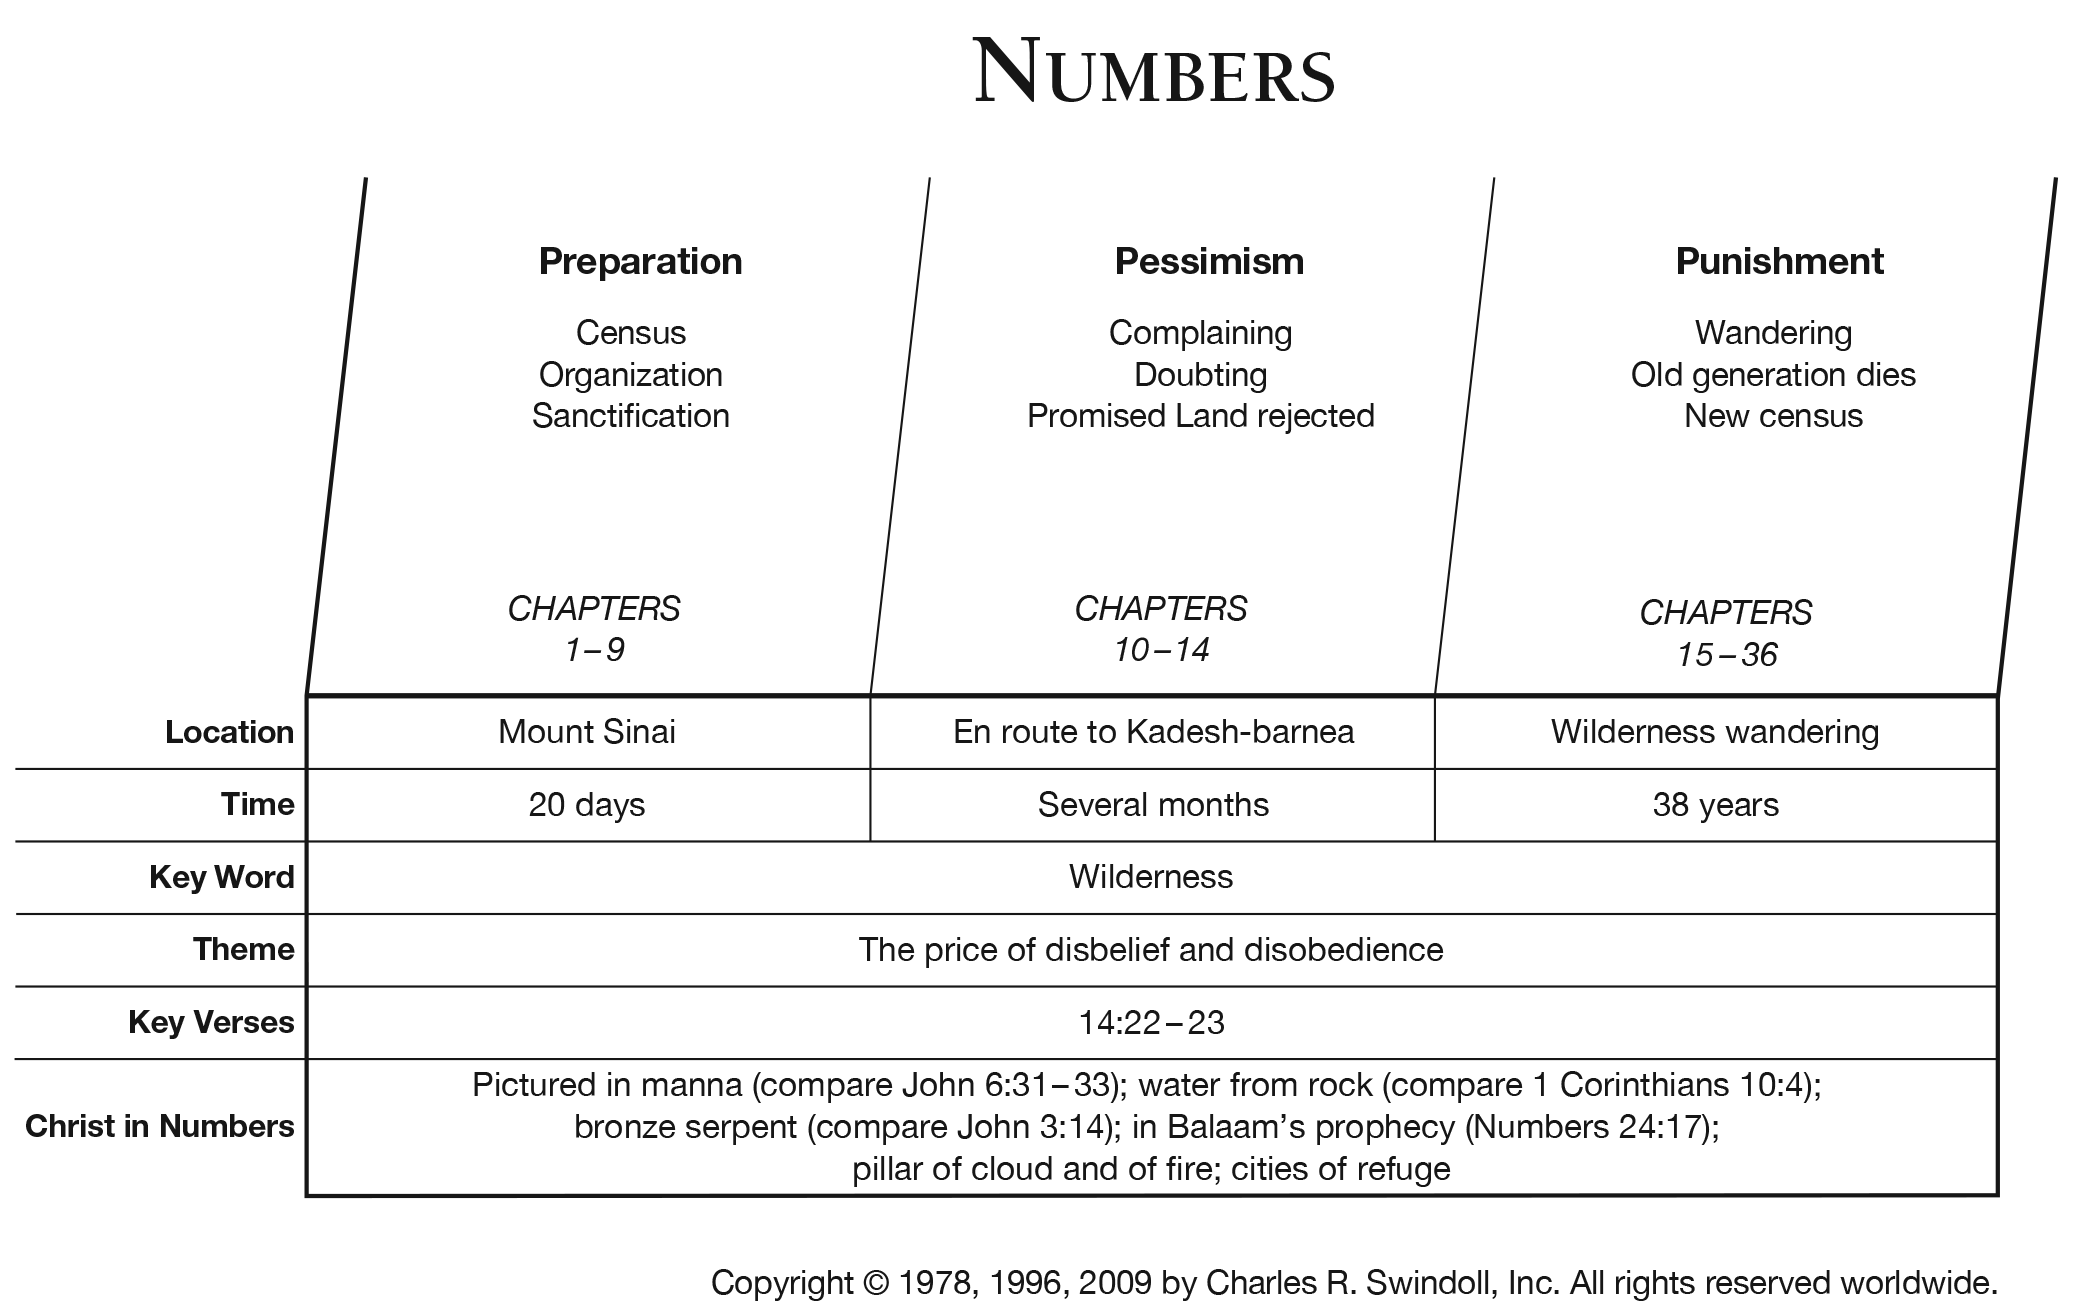
\includegraphics[scale=0.3, angle=90]{04OT-Numbers/References/Swindoll-Numbers.png}
\caption[Numbers by Swindoll]{Numbers by Swindoll}
\label{fig:Numbers by Swindoll}
\end{center}
\end{figure}

\newpage
\begin{figure}
\begin{center}
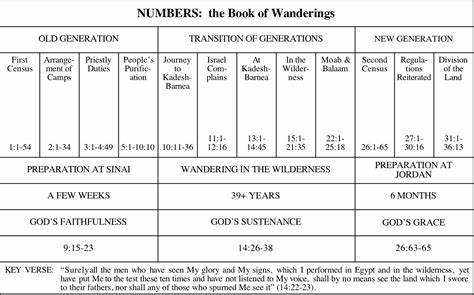
\includegraphics[scale=1.2, angle=90]{04OT-Numbers/References/Numbers.jpg}
\caption[Numbers by Unknown]{Numbers by Unknown}
\label{fig:Numbers by Unknown}
\end{center}
\end{figure}

\newpage
\begin{figure}
\begin{center}
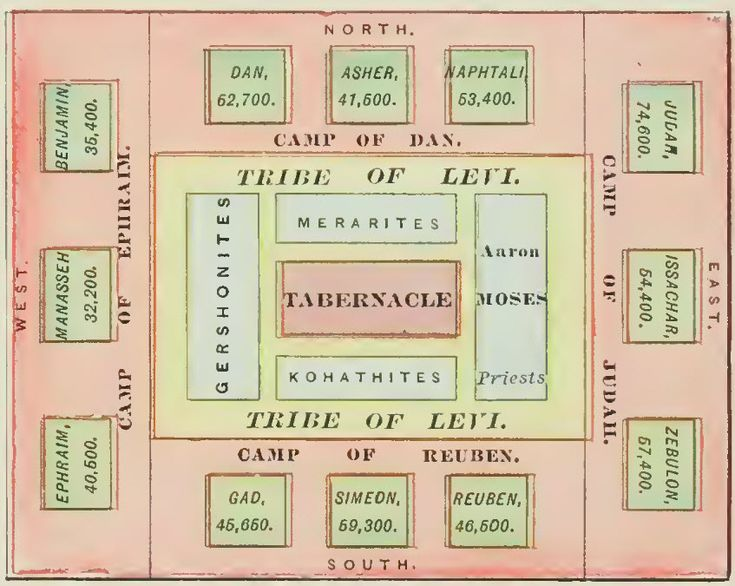
\includegraphics[scale=.8, angle=0]{04OT-Numbers/References/LayoutOfTribesAndTabernacle.jpg}
\caption[Layout of Tribes and Tabernacle]{Layout of Tribes and Tabernacle}
\label{fig:Layout of Tribes and Tabernacle}
\end{center}
\end{figure}


\chapter{Numbers 13}

\begin{figure}
  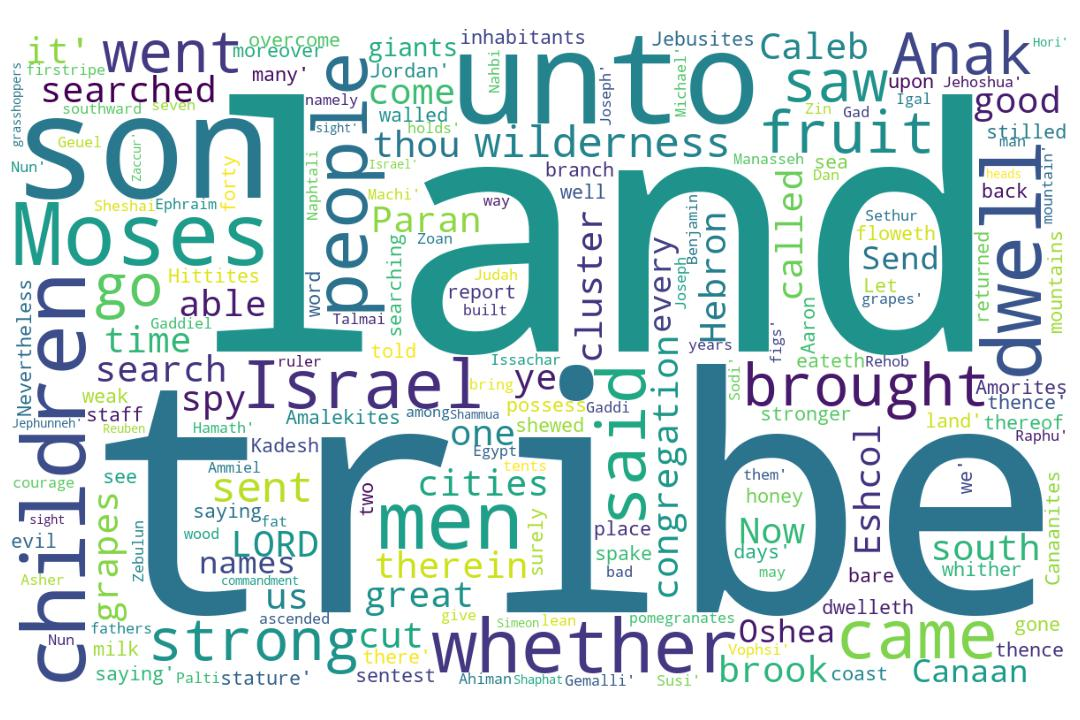
\includegraphics[width=\linewidth]{04OT-Numbers/Numbers13-WordCloud.jpg}
  \caption{Numbers 13 Word Cloud}
  \label{fig:Numbers 13 word Cloud}
\end{figure}



\marginpar{\scriptsize \centering \fcolorbox{bone}{lime}{\textbf{A 40-YEAR MISTAKE}}\\ (Numbers 13:1-33) \begin{compactenum}[I.][8]
    \item An \textbf{Inspection Tour} \index[scripture]{Numbers!Num 13:17}(Num 13:17) 
    \item An \textbf{Important Test} \index[scripture]{Numbers!Num 13:25}(Num 13:25) 
    \item \textbf{Impenetrable Towns} \index[scripture]{Numbers!Num 13:28}(Num 13:28) 
    \item \textbf{Insolent Transgressors} \index[scripture]{Numbers!Num 13:31}(Num 13:31) 
    \item People \textbf{Impressive \& Tall} \index[scripture]{Numbers!Num 13:32, 33}(Num 13:32, 33) 
    \item As \textbf{Insignificant Tourists} \index[scripture]{Numbers!Num 13:33}(Num 13:33) 
    \item An \textbf{Instructive Time} %\index[scripture]{Numbers!Numbers 13:17}(Numbers 13:17) 
\end{compactenum}}


\marginpar{\scriptsize \centering \fcolorbox{bone}{yellow}{\textbf{REBELLION AT KADESH}}\\ (Numbers 13:1-33) \begin{compactenum}[I.][8]
   \item The \textbf{Sending}  \index[scripture]{Numbers!Num 13:01}    (Num 13:1) 
   \item The \textbf{Search} \index[scripture]{Numbers!Num 13:01}  \index[scripture]{Numbers!Num 13:21}  \index[scripture]{Numbers!Num 13:25}\index[scripture]{Numbers!Num 13:32}  (Num 13:1, 21, 25, 32) 
   \item The \textbf{Sons}  \index[scripture]{Numbers!Num 13:04--15}    (Num 13:4--15) 
    \item The \textbf{Strength} of the Enemy \index[scripture]{Numbers!Num 13:18}\index[scripture]{Numbers!Num 13:28} \index[scripture]{Numbers!Num 13:31}  (Num 13:18, 28, 31) 
   \item The \textbf{Stature}  \index[scripture]{Numbers!Num 13:32}    (Num 13:32) 
   \item The \textbf{Sight}  of the Spies \index[scripture]{Numbers!Num 13:33}    (Num 13:33) 
  \item The \textbf{Significance} of Unbelief %\index[scripture]{Numbers!Num 13:01}    (Numbers 13:1) 
\end{compactenum}}

\marginpar{\scriptsize \centering \fcolorbox{bone}{black}{\textbf{\textcolor[cmyk]{0,0,0,0}{THE SPIES}}}\\ (Numbers 13:1-33) 
 \begin{compactenum}[I.][8]
   \item \textbf{Required} for the Mission \index[scripture]{Numbers!Num 13:02}    (Num 13:2) 
   \item \textbf{Represented} the Tribes \index[scripture]{Numbers!Num 13:02}    (Num 13:2) 
   \item \textbf{Recounted} the Enemies\index[scripture]{Numbers!Num 13:27--28}    (Num 13:27--28)
   \item \textbf{Rebelled}  \index[scripture]{Numbers!Num 13:31}    (Num 13:31)
   \item \textbf{Disregarded} the LORD \index[scripture]{Numbers!Num 13:31}    (Num 13:31)
   \item \textbf{Ruined} the chances to Enter the Land  ... for 40 years, and the death of over 600,000 men plus women and children and the strangers who were with them
   \item Didn't \textbf{Recognize} what they had with them
\end{compactenum}}

\marginpar{\scriptsize \centering \fcolorbox{bone}{blue}{\textcolor{white}{\textbf{THE SPIES DID NOT SEE}}}\\ (Numbers 13:1-33) 
 \begin{compactenum}[I.][8]
   \item The \textbf{Goodness} that Awaited \index[scripture]{Numbers!Num 13:32}    (Numbers 13:32) 
   \item The \textbf{Giants} Annihilated
   \item A \textbf{God} who is Awesome -- Bigger than the Giants 
   \item The \textbf{Grief} After their rebellion -- a defeat in the next chapter, a 40-year wait
   \item The \textbf{Guidance} that was Available
   \item  \textbf{Great} Victories Ahead
   \item The \textbf{Glory} of God Above all Else
\end{compactenum}}


\footnote{\textcolor[cmyk]{0.99998,1,0,0}{\hyperlink{TOC}{Return to end of Table of Contents.}}}\footnote{\href{https://audiobible.com/bible/numbers_13.html}{\textcolor[cmyk]{0.99998,1,0,0}{Numbers 13 Audio}}}\textcolor[cmyk]{0.99998,1,0,0}{And the LORD spake unto Moses, saying,}
[2] \textcolor[cmyk]{0.99998,1,0,0}{Send thou men, that they may search the land of Canaan, which I give unto the children of Israel: of every tribe of their fathers shall ye send a man, every one a ruler among them.}
[3] \textcolor[cmyk]{0.99998,1,0,0}{And Moses by the commandment of the LORD sent them from the wilderness of Paran: all those men \emph{were} heads of the children of Israel.}
[4] \textcolor[cmyk]{0.99998,1,0,0}{And these \emph{were} their names: of the tribe of Reuben, Shammua the \fcolorbox{bone}{bone}{son} of Zaccur.}
[5] \textcolor[cmyk]{0.99998,1,0,0}{Of the tribe of Simeon, Shaphat the \fcolorbox{bone}{bone}{son} of Hori.}
[6] \textcolor[cmyk]{0.99998,1,0,0}{Of the tribe of Judah, Caleb the \fcolorbox{bone}{bone}{son} of Jephunneh.}
[7] \textcolor[cmyk]{0.99998,1,0,0}{Of the tribe of Issachar, Igal the \fcolorbox{bone}{bone}{son} of Joseph.}
[8] \textcolor[cmyk]{0.99998,1,0,0}{Of the tribe of Ephraim, Oshea the \fcolorbox{bone}{bone}{son} of Nun.}
[9] \textcolor[cmyk]{0.99998,1,0,0}{Of the tribe of Benjamin, Palti the \fcolorbox{bone}{bone}{son} of Raphu.}
[10] \textcolor[cmyk]{0.99998,1,0,0}{Of the tribe of Zebulun, Gaddiel the \fcolorbox{bone}{bone}{son} of Sodi.}
[11] \textcolor[cmyk]{0.99998,1,0,0}{Of the tribe of Joseph, \emph{namely}, of the tribe of Manasseh, Gaddi the \fcolorbox{bone}{bone}{son} of Susi.}
[12] \textcolor[cmyk]{0.99998,1,0,0}{Of the tribe of Dan, Ammiel the \fcolorbox{bone}{bone}{son} of Gemalli.}
[13] \textcolor[cmyk]{0.99998,1,0,0}{Of the tribe of Asher, Sethur the \fcolorbox{bone}{bone}{son} of Michael.}
[14] \textcolor[cmyk]{0.99998,1,0,0}{Of the tribe of Naphtali, Nahbi the \fcolorbox{bone}{bone}{son} of Vophsi.}
[15] \textcolor[cmyk]{0.99998,1,0,0}{Of the tribe of Gad, Geuel the \fcolorbox{bone}{bone}{son} of Machi.}
[16] \textcolor[cmyk]{0.99998,1,0,0}{These \emph{are} the names of the men which Moses sent to spy out the land. And Moses called Oshea the \fcolorbox{bone}{bone}{son} of Nun Jehoshua.}\\
\\
\P \textcolor[cmyk]{0.99998,1,0,0}{And Moses sent them to spy out the land of Canaan, and said unto them, Get you up this \emph{way} southward, and go up into the mountain:}
[18] \textcolor[cmyk]{0.99998,1,0,0}{And see the land, what it \emph{is}; and the people that dwelleth therein, whether they \emph{be} strong or weak, few or many;}
[19] \textcolor[cmyk]{0.99998,1,0,0}{And what the land \emph{is} that they dwell in, whether it \emph{be} good or bad; and what cities \emph{they} \emph{be} that they dwell in, whether in tents, or in strong holds;}
[20] \textcolor[cmyk]{0.99998,1,0,0}{And what the land \emph{is}, whether it \emph{be} fat or lean, whether there be wood therein, or not. And be ye of good courage, and bring of the fruit of the land. Now the time \emph{was} the time of the firstripe grapes.}\\
\\
\P \textcolor[cmyk]{0.99998,1,0,0}{So they went up, and searched the land from the wilderness of Zin unto Rehob, as men come to Hamath.}
[22] \textcolor[cmyk]{0.99998,1,0,0}{And they ascended by the south, and came unto Hebron; where Ahiman, Sheshai, and Talmai, the children of Anak, \emph{were}. (Now Hebron was built seven years before Zoan in Egypt.)}
[23] \textcolor[cmyk]{0.99998,1,0,0}{And they came unto the brook of Eshcol, and cut down from thence a branch with one cluster of grapes, and they bare it between two upon a staff; and \emph{they} \emph{brought} of the pomegranates, and of the figs.}
[24] \textcolor[cmyk]{0.99998,1,0,0}{The place was called the brook Eshcol, because of the cluster of grapes which the children of Israel cut down from thence.}
[25] \textcolor[cmyk]{0.99998,1,0,0}{And they returned from searching of the land after forty days.}\\
\\
\P \textcolor[cmyk]{0.99998,1,0,0}{And they went and came to Moses, and to Aaron, and to all the congregation of the children of Israel, unto the wilderness of Paran, to Kadesh; and brought back word unto them, and unto all the congregation, and shewed them the fruit of the land.}
[27] \textcolor[cmyk]{0.99998,1,0,0}{And they told him, and said, We came unto the land whither thou sentest us, and surely it floweth with milk and honey; and this \emph{is} the fruit of it.}
[28] \textcolor[cmyk]{0.99998,1,0,0}{Nevertheless the people \emph{be} strong that dwell in the land, and the cities \emph{are} walled, \emph{and} very great: and moreover we saw the children of Anak there.}
[29] \textcolor[cmyk]{0.99998,1,0,0}{The Amalekites dwell in the land of the south: and the Hittites, and the Jebusites, and the Amorites, dwell in the mountains: and the Canaanites dwell by the sea, and by the coast of Jordan.}
[30] \textcolor[cmyk]{0.99998,1,0,0}{And Caleb stilled the people before Moses, and said, Let us go up at once, and possess it; for we are well able to overcome it.}
[31] \textcolor[cmyk]{0.99998,1,0,0}{But the men that went up with him said, We be not able to go up against the people; for they \emph{are} stronger than we.}
[32] \textcolor[cmyk]{0.99998,1,0,0}{And they brought up an evil report of the land which they had searched unto the children of Israel, saying, The land, through which we have gone to search it, \emph{is} a land that eateth up the inhabitants thereof; and all the people that we saw in it \emph{are} men of a great stature.}
[33] \textcolor[cmyk]{0.99998,1,0,0}{And there we saw the giants, the sons of Anak, \emph{which} \emph{come} of the giants: and we were in our own sight as grasshoppers, and so we were in their sight.}


\index[NWIV]{7!Numbers!Num 13:1}\index[AWIP]{And!Numbers!Num 13:1}\index[AWIP]{the!Numbers!Num 13:1}\index[AWIP]{LORD!Numbers!Num 13:1}\index[AWIP]{spake!Numbers!Num 13:1}\index[AWIP]{unto!Numbers!Num 13:1}\index[AWIP]{Moses!Numbers!Num 13:1}\index[AWIP]{saying!Numbers!Num 13:1}

\index[NWIV]{36!Numbers!Num 13:2}\index[AWIP]{Send!Numbers!Num 13:2}\index[AWIP]{thou!Numbers!Num 13:2}\index[AWIP]{men!Numbers!Num 13:2}\index[AWIP]{that!Numbers!Num 13:2}\index[AWIP]{they!Numbers!Num 13:2}\index[AWIP]{may!Numbers!Num 13:2}\index[AWIP]{search!Numbers!Num 13:2}\index[AWIP]{the!Numbers!Num 13:2}\index[AWIP]{the!Numbers!Num 13:2 (2)}\index[AWIP]{land!Numbers!Num 13:2}\index[AWIP]{of!Numbers!Num 13:2}\index[AWIP]{of!Numbers!Num 13:2 (2)}\index[AWIP]{of!Numbers!Num 13:2 (3)}\index[AWIP]{of!Numbers!Num 13:2 (4)}\index[AWIP]{Canaan!Numbers!Num 13:2}\index[AWIP]{which!Numbers!Num 13:2}\index[AWIP]{I!Numbers!Num 13:2}\index[AWIP]{give!Numbers!Num 13:2}\index[AWIP]{unto!Numbers!Num 13:2}\index[AWIP]{children!Numbers!Num 13:2}\index[AWIP]{Israel!Numbers!Num 13:2}\index[AWIP]{every!Numbers!Num 13:2}\index[AWIP]{every!Numbers!Num 13:2 (2)}\index[AWIP]{tribe!Numbers!Num 13:2}\index[AWIP]{their!Numbers!Num 13:2}\index[AWIP]{fathers!Numbers!Num 13:2}\index[AWIP]{shall!Numbers!Num 13:2}\index[AWIP]{ye!Numbers!Num 13:2}\index[AWIP]{send!Numbers!Num 13:2}\index[AWIP]{a!Numbers!Num 13:2}\index[AWIP]{a!Numbers!Num 13:2 (2)}\index[AWIP]{man!Numbers!Num 13:2}\index[AWIP]{one!Numbers!Num 13:2}\index[AWIP]{ruler!Numbers!Num 13:2}\index[AWIP]{among!Numbers!Num 13:2}\index[AWIP]{them!Numbers!Num 13:2}

\index[NWIV]{25!Numbers!Num 13:3}\index[AWIP]{And!Numbers!Num 13:3}\index[AWIP]{Moses!Numbers!Num 13:3}\index[AWIP]{by!Numbers!Num 13:3}\index[AWIP]{the!Numbers!Num 13:3}\index[AWIP]{the!Numbers!Num 13:3 (2)}\index[AWIP]{the!Numbers!Num 13:3 (3)}\index[AWIP]{the!Numbers!Num 13:3 (4)}\index[AWIP]{commandment!Numbers!Num 13:3}\index[AWIP]{of!Numbers!Num 13:3}\index[AWIP]{of!Numbers!Num 13:3 (2)}\index[AWIP]{of!Numbers!Num 13:3 (3)}\index[AWIP]{of!Numbers!Num 13:3 (4)}\index[AWIP]{LORD!Numbers!Num 13:3}\index[AWIP]{sent!Numbers!Num 13:3}\index[AWIP]{them!Numbers!Num 13:3}\index[AWIP]{from!Numbers!Num 13:3}\index[AWIP]{wilderness!Numbers!Num 13:3}\index[AWIP]{Paran!Numbers!Num 13:3}\index[AWIP]{all!Numbers!Num 13:3}\index[AWIP]{those!Numbers!Num 13:3}\index[AWIP]{men!Numbers!Num 13:3}\index[AWIP]{\emph{were}!Numbers!Num 13:3}\index[AWIP]{heads!Numbers!Num 13:3}\index[AWIP]{children!Numbers!Num 13:3}\index[AWIP]{Israel!Numbers!Num 13:3}\index[AWIP]{\emph{were}!Numbers!Num 13:3}

\index[NWIV]{15!Numbers!Num 13:4}\index[AWIP]{And!Numbers!Num 13:4}\index[AWIP]{these!Numbers!Num 13:4}\index[AWIP]{\emph{were}!Numbers!Num 13:4}\index[AWIP]{their!Numbers!Num 13:4}\index[AWIP]{names!Numbers!Num 13:4}\index[AWIP]{of!Numbers!Num 13:4}\index[AWIP]{of!Numbers!Num 13:4 (2)}\index[AWIP]{of!Numbers!Num 13:4 (3)}\index[AWIP]{the!Numbers!Num 13:4}\index[AWIP]{the!Numbers!Num 13:4 (2)}\index[AWIP]{tribe!Numbers!Num 13:4}\index[AWIP]{Reuben!Numbers!Num 13:4}\index[AWIP]{Shammua!Numbers!Num 13:4}\index[AWIP]{son!Numbers!Num 13:4}\index[AWIP]{Zaccur!Numbers!Num 13:4}\index[AWIP]{\emph{were}!Numbers!Num 13:4}

\index[NWIV]{10!Numbers!Num 13:5}\index[AWIP]{Of!Numbers!Num 13:5}\index[AWIP]{the!Numbers!Num 13:5}\index[AWIP]{the!Numbers!Num 13:5 (2)}\index[AWIP]{tribe!Numbers!Num 13:5}\index[AWIP]{of!Numbers!Num 13:5}\index[AWIP]{of!Numbers!Num 13:5 (2)}\index[AWIP]{Simeon!Numbers!Num 13:5}\index[AWIP]{Shaphat!Numbers!Num 13:5}\index[AWIP]{son!Numbers!Num 13:5}\index[AWIP]{Hori!Numbers!Num 13:5}

\index[NWIV]{10!Numbers!Num 13:6}\index[AWIP]{Of!Numbers!Num 13:6}\index[AWIP]{the!Numbers!Num 13:6}\index[AWIP]{the!Numbers!Num 13:6 (2)}\index[AWIP]{tribe!Numbers!Num 13:6}\index[AWIP]{of!Numbers!Num 13:6}\index[AWIP]{of!Numbers!Num 13:6 (2)}\index[AWIP]{Judah!Numbers!Num 13:6}\index[AWIP]{Caleb!Numbers!Num 13:6}\index[AWIP]{son!Numbers!Num 13:6}\index[AWIP]{Jephunneh!Numbers!Num 13:6}

\index[NWIV]{10!Numbers!Num 13:7}\index[AWIP]{Of!Numbers!Num 13:7}\index[AWIP]{the!Numbers!Num 13:7}\index[AWIP]{the!Numbers!Num 13:7 (2)}\index[AWIP]{tribe!Numbers!Num 13:7}\index[AWIP]{of!Numbers!Num 13:7}\index[AWIP]{of!Numbers!Num 13:7 (2)}\index[AWIP]{Issachar!Numbers!Num 13:7}\index[AWIP]{Igal!Numbers!Num 13:7}\index[AWIP]{son!Numbers!Num 13:7}\index[AWIP]{Joseph!Numbers!Num 13:7}

\index[NWIV]{10!Numbers!Num 13:8}\index[AWIP]{Of!Numbers!Num 13:8}\index[AWIP]{the!Numbers!Num 13:8}\index[AWIP]{the!Numbers!Num 13:8 (2)}\index[AWIP]{tribe!Numbers!Num 13:8}\index[AWIP]{of!Numbers!Num 13:8}\index[AWIP]{of!Numbers!Num 13:8 (2)}\index[AWIP]{Ephraim!Numbers!Num 13:8}\index[AWIP]{Oshea!Numbers!Num 13:8}\index[AWIP]{son!Numbers!Num 13:8}\index[AWIP]{Nun!Numbers!Num 13:8}

\index[NWIV]{10!Numbers!Num 13:9}\index[AWIP]{Of!Numbers!Num 13:9}\index[AWIP]{the!Numbers!Num 13:9}\index[AWIP]{the!Numbers!Num 13:9 (2)}\index[AWIP]{tribe!Numbers!Num 13:9}\index[AWIP]{of!Numbers!Num 13:9}\index[AWIP]{of!Numbers!Num 13:9 (2)}\index[AWIP]{Benjamin!Numbers!Num 13:9}\index[AWIP]{Palti!Numbers!Num 13:9}\index[AWIP]{son!Numbers!Num 13:9}\index[AWIP]{Raphu!Numbers!Num 13:9}

\index[NWIV]{10!Numbers!Num 13:10}\index[AWIP]{Of!Numbers!Num 13:10}\index[AWIP]{the!Numbers!Num 13:10}\index[AWIP]{the!Numbers!Num 13:10 (2)}\index[AWIP]{tribe!Numbers!Num 13:10}\index[AWIP]{of!Numbers!Num 13:10}\index[AWIP]{of!Numbers!Num 13:10 (2)}\index[AWIP]{Zebulun!Numbers!Num 13:10}\index[AWIP]{Gaddiel!Numbers!Num 13:10}\index[AWIP]{son!Numbers!Num 13:10}\index[AWIP]{Sodi!Numbers!Num 13:10}

\index[NWIV]{16!Numbers!Num 13:11}\index[AWIP]{Of!Numbers!Num 13:11}\index[AWIP]{the!Numbers!Num 13:11}\index[AWIP]{the!Numbers!Num 13:11 (2)}\index[AWIP]{the!Numbers!Num 13:11 (3)}\index[AWIP]{tribe!Numbers!Num 13:11}\index[AWIP]{tribe!Numbers!Num 13:11 (2)}\index[AWIP]{of!Numbers!Num 13:11}\index[AWIP]{of!Numbers!Num 13:11 (2)}\index[AWIP]{of!Numbers!Num 13:11 (3)}\index[AWIP]{of!Numbers!Num 13:11 (4)}\index[AWIP]{Joseph!Numbers!Num 13:11}\index[AWIP]{\emph{namely}!Numbers!Num 13:11}\index[AWIP]{Manasseh!Numbers!Num 13:11}\index[AWIP]{Gaddi!Numbers!Num 13:11}\index[AWIP]{son!Numbers!Num 13:11}\index[AWIP]{Susi!Numbers!Num 13:11}\index[AWIP]{\emph{namely}!Numbers!Num 13:11}

\index[NWIV]{10!Numbers!Num 13:12}\index[AWIP]{Of!Numbers!Num 13:12}\index[AWIP]{the!Numbers!Num 13:12}\index[AWIP]{the!Numbers!Num 13:12 (2)}\index[AWIP]{tribe!Numbers!Num 13:12}\index[AWIP]{of!Numbers!Num 13:12}\index[AWIP]{of!Numbers!Num 13:12 (2)}\index[AWIP]{Dan!Numbers!Num 13:12}\index[AWIP]{Ammiel!Numbers!Num 13:12}\index[AWIP]{son!Numbers!Num 13:12}\index[AWIP]{Gemalli!Numbers!Num 13:12}

\index[NWIV]{10!Numbers!Num 13:13}\index[AWIP]{Of!Numbers!Num 13:13}\index[AWIP]{the!Numbers!Num 13:13}\index[AWIP]{the!Numbers!Num 13:13 (2)}\index[AWIP]{tribe!Numbers!Num 13:13}\index[AWIP]{of!Numbers!Num 13:13}\index[AWIP]{of!Numbers!Num 13:13 (2)}\index[AWIP]{Asher!Numbers!Num 13:13}\index[AWIP]{Sethur!Numbers!Num 13:13}\index[AWIP]{son!Numbers!Num 13:13}\index[AWIP]{Michael!Numbers!Num 13:13}

\index[NWIV]{10!Numbers!Num 13:14}\index[AWIP]{Of!Numbers!Num 13:14}\index[AWIP]{the!Numbers!Num 13:14}\index[AWIP]{the!Numbers!Num 13:14 (2)}\index[AWIP]{tribe!Numbers!Num 13:14}\index[AWIP]{of!Numbers!Num 13:14}\index[AWIP]{of!Numbers!Num 13:14 (2)}\index[AWIP]{Naphtali!Numbers!Num 13:14}\index[AWIP]{Nahbi!Numbers!Num 13:14}\index[AWIP]{son!Numbers!Num 13:14}\index[AWIP]{Vophsi!Numbers!Num 13:14}

\index[NWIV]{10!Numbers!Num 13:15}\index[AWIP]{Of!Numbers!Num 13:15}\index[AWIP]{the!Numbers!Num 13:15}\index[AWIP]{the!Numbers!Num 13:15 (2)}\index[AWIP]{tribe!Numbers!Num 13:15}\index[AWIP]{of!Numbers!Num 13:15}\index[AWIP]{of!Numbers!Num 13:15 (2)}\index[AWIP]{Gad!Numbers!Num 13:15}\index[AWIP]{Geuel!Numbers!Num 13:15}\index[AWIP]{son!Numbers!Num 13:15}\index[AWIP]{Machi!Numbers!Num 13:15}

\index[NWIV]{24!Numbers!Num 13:16}\index[AWIP]{These!Numbers!Num 13:16}\index[AWIP]{\emph{are}!Numbers!Num 13:16}\index[AWIP]{the!Numbers!Num 13:16}\index[AWIP]{the!Numbers!Num 13:16 (2)}\index[AWIP]{the!Numbers!Num 13:16 (3)}\index[AWIP]{the!Numbers!Num 13:16 (4)}\index[AWIP]{names!Numbers!Num 13:16}\index[AWIP]{of!Numbers!Num 13:16}\index[AWIP]{of!Numbers!Num 13:16 (2)}\index[AWIP]{men!Numbers!Num 13:16}\index[AWIP]{which!Numbers!Num 13:16}\index[AWIP]{Moses!Numbers!Num 13:16}\index[AWIP]{Moses!Numbers!Num 13:16 (2)}\index[AWIP]{sent!Numbers!Num 13:16}\index[AWIP]{to!Numbers!Num 13:16}\index[AWIP]{spy!Numbers!Num 13:16}\index[AWIP]{out!Numbers!Num 13:16}\index[AWIP]{land!Numbers!Num 13:16}\index[AWIP]{And!Numbers!Num 13:16}\index[AWIP]{called!Numbers!Num 13:16}\index[AWIP]{Oshea!Numbers!Num 13:16}\index[AWIP]{son!Numbers!Num 13:16}\index[AWIP]{Nun!Numbers!Num 13:16}\index[AWIP]{Jehoshua!Numbers!Num 13:16}\index[AWIP]{\emph{are}!Numbers!Num 13:16}

\index[NWIV]{27!Numbers!Num 13:17}\index[AWIP]{And!Numbers!Num 13:17}\index[AWIP]{Moses!Numbers!Num 13:17}\index[AWIP]{sent!Numbers!Num 13:17}\index[AWIP]{them!Numbers!Num 13:17}\index[AWIP]{them!Numbers!Num 13:17 (2)}\index[AWIP]{to!Numbers!Num 13:17}\index[AWIP]{spy!Numbers!Num 13:17}\index[AWIP]{out!Numbers!Num 13:17}\index[AWIP]{the!Numbers!Num 13:17}\index[AWIP]{the!Numbers!Num 13:17 (2)}\index[AWIP]{land!Numbers!Num 13:17}\index[AWIP]{of!Numbers!Num 13:17}\index[AWIP]{Canaan!Numbers!Num 13:17}\index[AWIP]{and!Numbers!Num 13:17}\index[AWIP]{and!Numbers!Num 13:17 (2)}\index[AWIP]{said!Numbers!Num 13:17}\index[AWIP]{unto!Numbers!Num 13:17}\index[AWIP]{Get!Numbers!Num 13:17}\index[AWIP]{you!Numbers!Num 13:17}\index[AWIP]{up!Numbers!Num 13:17}\index[AWIP]{up!Numbers!Num 13:17 (2)}\index[AWIP]{this!Numbers!Num 13:17}\index[AWIP]{\emph{way}!Numbers!Num 13:17}\index[AWIP]{southward!Numbers!Num 13:17}\index[AWIP]{go!Numbers!Num 13:17}\index[AWIP]{into!Numbers!Num 13:17}\index[AWIP]{mountain!Numbers!Num 13:17}\index[AWIP]{\emph{way}!Numbers!Num 13:17}

\index[NWIV]{22!Numbers!Num 13:18}\index[AWIP]{And!Numbers!Num 13:18}\index[AWIP]{see!Numbers!Num 13:18}\index[AWIP]{the!Numbers!Num 13:18}\index[AWIP]{the!Numbers!Num 13:18 (2)}\index[AWIP]{land!Numbers!Num 13:18}\index[AWIP]{what!Numbers!Num 13:18}\index[AWIP]{it!Numbers!Num 13:18}\index[AWIP]{\emph{is}!Numbers!Num 13:18}\index[AWIP]{and!Numbers!Num 13:18}\index[AWIP]{people!Numbers!Num 13:18}\index[AWIP]{that!Numbers!Num 13:18}\index[AWIP]{dwelleth!Numbers!Num 13:18}\index[AWIP]{therein!Numbers!Num 13:18}\index[AWIP]{whether!Numbers!Num 13:18}\index[AWIP]{they!Numbers!Num 13:18}\index[AWIP]{\emph{be}!Numbers!Num 13:18}\index[AWIP]{strong!Numbers!Num 13:18}\index[AWIP]{or!Numbers!Num 13:18}\index[AWIP]{or!Numbers!Num 13:18 (2)}\index[AWIP]{weak!Numbers!Num 13:18}\index[AWIP]{few!Numbers!Num 13:18}\index[AWIP]{many!Numbers!Num 13:18}\index[AWIP]{\emph{is}!Numbers!Num 13:18}\index[AWIP]{\emph{be}!Numbers!Num 13:18}

\index[NWIV]{31!Numbers!Num 13:19}\index[AWIP]{And!Numbers!Num 13:19}\index[AWIP]{what!Numbers!Num 13:19}\index[AWIP]{what!Numbers!Num 13:19 (2)}\index[AWIP]{the!Numbers!Num 13:19}\index[AWIP]{land!Numbers!Num 13:19}\index[AWIP]{\emph{is}!Numbers!Num 13:19}\index[AWIP]{that!Numbers!Num 13:19}\index[AWIP]{that!Numbers!Num 13:19 (2)}\index[AWIP]{they!Numbers!Num 13:19}\index[AWIP]{they!Numbers!Num 13:19 (2)}\index[AWIP]{dwell!Numbers!Num 13:19}\index[AWIP]{dwell!Numbers!Num 13:19 (2)}\index[AWIP]{in!Numbers!Num 13:19}\index[AWIP]{in!Numbers!Num 13:19 (2)}\index[AWIP]{in!Numbers!Num 13:19 (3)}\index[AWIP]{in!Numbers!Num 13:19 (4)}\index[AWIP]{whether!Numbers!Num 13:19}\index[AWIP]{whether!Numbers!Num 13:19 (2)}\index[AWIP]{it!Numbers!Num 13:19}\index[AWIP]{\emph{be}!Numbers!Num 13:19}\index[AWIP]{\emph{be}!Numbers!Num 13:19 (2)}\index[AWIP]{good!Numbers!Num 13:19}\index[AWIP]{or!Numbers!Num 13:19}\index[AWIP]{or!Numbers!Num 13:19 (2)}\index[AWIP]{bad!Numbers!Num 13:19}\index[AWIP]{and!Numbers!Num 13:19}\index[AWIP]{cities!Numbers!Num 13:19}\index[AWIP]{\emph{they}!Numbers!Num 13:19}\index[AWIP]{tents!Numbers!Num 13:19}\index[AWIP]{strong!Numbers!Num 13:19}\index[AWIP]{holds!Numbers!Num 13:19}\index[AWIP]{\emph{is}!Numbers!Num 13:19}\index[AWIP]{\emph{be}!Numbers!Num 13:19}\index[AWIP]{\emph{be}!Numbers!Num 13:19 (2)}\index[AWIP]{\emph{they}!Numbers!Num 13:19}

\index[NWIV]{42!Numbers!Num 13:20}\index[AWIP]{And!Numbers!Num 13:20}\index[AWIP]{And!Numbers!Num 13:20 (2)}\index[AWIP]{what!Numbers!Num 13:20}\index[AWIP]{the!Numbers!Num 13:20}\index[AWIP]{the!Numbers!Num 13:20 (2)}\index[AWIP]{the!Numbers!Num 13:20 (3)}\index[AWIP]{the!Numbers!Num 13:20 (4)}\index[AWIP]{the!Numbers!Num 13:20 (5)}\index[AWIP]{the!Numbers!Num 13:20 (6)}\index[AWIP]{land!Numbers!Num 13:20}\index[AWIP]{land!Numbers!Num 13:20 (2)}\index[AWIP]{\emph{is}!Numbers!Num 13:20}\index[AWIP]{whether!Numbers!Num 13:20}\index[AWIP]{whether!Numbers!Num 13:20 (2)}\index[AWIP]{it!Numbers!Num 13:20}\index[AWIP]{\emph{be}!Numbers!Num 13:20}\index[AWIP]{fat!Numbers!Num 13:20}\index[AWIP]{or!Numbers!Num 13:20}\index[AWIP]{or!Numbers!Num 13:20 (2)}\index[AWIP]{lean!Numbers!Num 13:20}\index[AWIP]{there!Numbers!Num 13:20}\index[AWIP]{be!Numbers!Num 13:20}\index[AWIP]{be!Numbers!Num 13:20 (2)}\index[AWIP]{wood!Numbers!Num 13:20}\index[AWIP]{therein!Numbers!Num 13:20}\index[AWIP]{not!Numbers!Num 13:20}\index[AWIP]{ye!Numbers!Num 13:20}\index[AWIP]{of!Numbers!Num 13:20}\index[AWIP]{of!Numbers!Num 13:20 (2)}\index[AWIP]{of!Numbers!Num 13:20 (3)}\index[AWIP]{of!Numbers!Num 13:20 (4)}\index[AWIP]{good!Numbers!Num 13:20}\index[AWIP]{courage!Numbers!Num 13:20}\index[AWIP]{and!Numbers!Num 13:20}\index[AWIP]{bring!Numbers!Num 13:20}\index[AWIP]{fruit!Numbers!Num 13:20}\index[AWIP]{Now!Numbers!Num 13:20}\index[AWIP]{time!Numbers!Num 13:20}\index[AWIP]{time!Numbers!Num 13:20 (2)}\index[AWIP]{\emph{was}!Numbers!Num 13:20}\index[AWIP]{firstripe!Numbers!Num 13:20}\index[AWIP]{grapes!Numbers!Num 13:20}\index[AWIP]{\emph{is}!Numbers!Num 13:20}\index[AWIP]{\emph{be}!Numbers!Num 13:20}\index[AWIP]{\emph{was}!Numbers!Num 13:20}

\index[NWIV]{20!Numbers!Num 13:21}\index[AWIP]{So!Numbers!Num 13:21}\index[AWIP]{they!Numbers!Num 13:21}\index[AWIP]{went!Numbers!Num 13:21}\index[AWIP]{up!Numbers!Num 13:21}\index[AWIP]{and!Numbers!Num 13:21}\index[AWIP]{searched!Numbers!Num 13:21}\index[AWIP]{the!Numbers!Num 13:21}\index[AWIP]{the!Numbers!Num 13:21 (2)}\index[AWIP]{land!Numbers!Num 13:21}\index[AWIP]{from!Numbers!Num 13:21}\index[AWIP]{wilderness!Numbers!Num 13:21}\index[AWIP]{of!Numbers!Num 13:21}\index[AWIP]{Zin!Numbers!Num 13:21}\index[AWIP]{unto!Numbers!Num 13:21}\index[AWIP]{Rehob!Numbers!Num 13:21}\index[AWIP]{as!Numbers!Num 13:21}\index[AWIP]{men!Numbers!Num 13:21}\index[AWIP]{come!Numbers!Num 13:21}\index[AWIP]{to!Numbers!Num 13:21}\index[AWIP]{Hamath!Numbers!Num 13:21}

\index[NWIV]{30!Numbers!Num 13:22}\index[AWIP]{And!Numbers!Num 13:22}\index[AWIP]{they!Numbers!Num 13:22}\index[AWIP]{ascended!Numbers!Num 13:22}\index[AWIP]{by!Numbers!Num 13:22}\index[AWIP]{the!Numbers!Num 13:22}\index[AWIP]{the!Numbers!Num 13:22 (2)}\index[AWIP]{south!Numbers!Num 13:22}\index[AWIP]{and!Numbers!Num 13:22}\index[AWIP]{and!Numbers!Num 13:22 (2)}\index[AWIP]{came!Numbers!Num 13:22}\index[AWIP]{unto!Numbers!Num 13:22}\index[AWIP]{Hebron!Numbers!Num 13:22}\index[AWIP]{Hebron!Numbers!Num 13:22 (2)}\index[AWIP]{where!Numbers!Num 13:22}\index[AWIP]{Ahiman!Numbers!Num 13:22}\index[AWIP]{Sheshai!Numbers!Num 13:22}\index[AWIP]{Talmai!Numbers!Num 13:22}\index[AWIP]{children!Numbers!Num 13:22}\index[AWIP]{of!Numbers!Num 13:22}\index[AWIP]{Anak!Numbers!Num 13:22}\index[AWIP]{\emph{were}!Numbers!Num 13:22}\index[AWIP]{(Now!Numbers!Num 13:22}\index[AWIP]{was!Numbers!Num 13:22}\index[AWIP]{built!Numbers!Num 13:22}\index[AWIP]{seven!Numbers!Num 13:22}\index[AWIP]{years!Numbers!Num 13:22}\index[AWIP]{before!Numbers!Num 13:22}\index[AWIP]{Zoan!Numbers!Num 13:22}\index[AWIP]{in!Numbers!Num 13:22}\index[AWIP]{Egypt)!Numbers!Num 13:22}\index[AWIP]{\emph{were}!Numbers!Num 13:22}

\index[NWIV]{39!Numbers!Num 13:23}\index[AWIP]{And!Numbers!Num 13:23}\index[AWIP]{they!Numbers!Num 13:23}\index[AWIP]{they!Numbers!Num 13:23 (2)}\index[AWIP]{came!Numbers!Num 13:23}\index[AWIP]{unto!Numbers!Num 13:23}\index[AWIP]{the!Numbers!Num 13:23}\index[AWIP]{the!Numbers!Num 13:23 (2)}\index[AWIP]{the!Numbers!Num 13:23 (3)}\index[AWIP]{brook!Numbers!Num 13:23}\index[AWIP]{of!Numbers!Num 13:23}\index[AWIP]{of!Numbers!Num 13:23 (2)}\index[AWIP]{of!Numbers!Num 13:23 (3)}\index[AWIP]{of!Numbers!Num 13:23 (4)}\index[AWIP]{Eshcol!Numbers!Num 13:23}\index[AWIP]{and!Numbers!Num 13:23}\index[AWIP]{and!Numbers!Num 13:23 (2)}\index[AWIP]{and!Numbers!Num 13:23 (3)}\index[AWIP]{and!Numbers!Num 13:23 (4)}\index[AWIP]{cut!Numbers!Num 13:23}\index[AWIP]{down!Numbers!Num 13:23}\index[AWIP]{from!Numbers!Num 13:23}\index[AWIP]{thence!Numbers!Num 13:23}\index[AWIP]{a!Numbers!Num 13:23}\index[AWIP]{a!Numbers!Num 13:23 (2)}\index[AWIP]{branch!Numbers!Num 13:23}\index[AWIP]{with!Numbers!Num 13:23}\index[AWIP]{one!Numbers!Num 13:23}\index[AWIP]{cluster!Numbers!Num 13:23}\index[AWIP]{grapes!Numbers!Num 13:23}\index[AWIP]{bare!Numbers!Num 13:23}\index[AWIP]{it!Numbers!Num 13:23}\index[AWIP]{between!Numbers!Num 13:23}\index[AWIP]{two!Numbers!Num 13:23}\index[AWIP]{upon!Numbers!Num 13:23}\index[AWIP]{staff!Numbers!Num 13:23}\index[AWIP]{\emph{they}!Numbers!Num 13:23}\index[AWIP]{\emph{brought}!Numbers!Num 13:23}\index[AWIP]{pomegranates!Numbers!Num 13:23}\index[AWIP]{figs!Numbers!Num 13:23}\index[AWIP]{\emph{they}!Numbers!Num 13:23}\index[AWIP]{\emph{brought}!Numbers!Num 13:23}

\index[NWIV]{22!Numbers!Num 13:24}\index[AWIP]{The!Numbers!Num 13:24}\index[AWIP]{place!Numbers!Num 13:24}\index[AWIP]{was!Numbers!Num 13:24}\index[AWIP]{called!Numbers!Num 13:24}\index[AWIP]{the!Numbers!Num 13:24}\index[AWIP]{the!Numbers!Num 13:24 (2)}\index[AWIP]{the!Numbers!Num 13:24 (3)}\index[AWIP]{brook!Numbers!Num 13:24}\index[AWIP]{Eshcol!Numbers!Num 13:24}\index[AWIP]{because!Numbers!Num 13:24}\index[AWIP]{of!Numbers!Num 13:24}\index[AWIP]{of!Numbers!Num 13:24 (2)}\index[AWIP]{of!Numbers!Num 13:24 (3)}\index[AWIP]{cluster!Numbers!Num 13:24}\index[AWIP]{grapes!Numbers!Num 13:24}\index[AWIP]{which!Numbers!Num 13:24}\index[AWIP]{children!Numbers!Num 13:24}\index[AWIP]{Israel!Numbers!Num 13:24}\index[AWIP]{cut!Numbers!Num 13:24}\index[AWIP]{down!Numbers!Num 13:24}\index[AWIP]{from!Numbers!Num 13:24}\index[AWIP]{thence!Numbers!Num 13:24}

\index[NWIV]{11!Numbers!Num 13:25}\index[AWIP]{And!Numbers!Num 13:25}\index[AWIP]{they!Numbers!Num 13:25}\index[AWIP]{returned!Numbers!Num 13:25}\index[AWIP]{from!Numbers!Num 13:25}\index[AWIP]{searching!Numbers!Num 13:25}\index[AWIP]{of!Numbers!Num 13:25}\index[AWIP]{the!Numbers!Num 13:25}\index[AWIP]{land!Numbers!Num 13:25}\index[AWIP]{after!Numbers!Num 13:25}\index[AWIP]{forty!Numbers!Num 13:25}\index[AWIP]{days!Numbers!Num 13:25}

\index[NWIV]{46!Numbers!Num 13:26}\index[AWIP]{And!Numbers!Num 13:26}\index[AWIP]{they!Numbers!Num 13:26}\index[AWIP]{went!Numbers!Num 13:26}\index[AWIP]{and!Numbers!Num 13:26}\index[AWIP]{and!Numbers!Num 13:26 (2)}\index[AWIP]{and!Numbers!Num 13:26 (3)}\index[AWIP]{and!Numbers!Num 13:26 (4)}\index[AWIP]{and!Numbers!Num 13:26 (5)}\index[AWIP]{and!Numbers!Num 13:26 (6)}\index[AWIP]{came!Numbers!Num 13:26}\index[AWIP]{to!Numbers!Num 13:26}\index[AWIP]{to!Numbers!Num 13:26 (2)}\index[AWIP]{to!Numbers!Num 13:26 (3)}\index[AWIP]{to!Numbers!Num 13:26 (4)}\index[AWIP]{Moses!Numbers!Num 13:26}\index[AWIP]{Aaron!Numbers!Num 13:26}\index[AWIP]{all!Numbers!Num 13:26}\index[AWIP]{all!Numbers!Num 13:26 (2)}\index[AWIP]{the!Numbers!Num 13:26}\index[AWIP]{the!Numbers!Num 13:26 (2)}\index[AWIP]{the!Numbers!Num 13:26 (3)}\index[AWIP]{the!Numbers!Num 13:26 (4)}\index[AWIP]{the!Numbers!Num 13:26 (5)}\index[AWIP]{the!Numbers!Num 13:26 (6)}\index[AWIP]{congregation!Numbers!Num 13:26}\index[AWIP]{congregation!Numbers!Num 13:26 (2)}\index[AWIP]{of!Numbers!Num 13:26}\index[AWIP]{of!Numbers!Num 13:26 (2)}\index[AWIP]{of!Numbers!Num 13:26 (3)}\index[AWIP]{of!Numbers!Num 13:26 (4)}\index[AWIP]{children!Numbers!Num 13:26}\index[AWIP]{Israel!Numbers!Num 13:26}\index[AWIP]{unto!Numbers!Num 13:26}\index[AWIP]{unto!Numbers!Num 13:26 (2)}\index[AWIP]{unto!Numbers!Num 13:26 (3)}\index[AWIP]{wilderness!Numbers!Num 13:26}\index[AWIP]{Paran!Numbers!Num 13:26}\index[AWIP]{Kadesh!Numbers!Num 13:26}\index[AWIP]{brought!Numbers!Num 13:26}\index[AWIP]{back!Numbers!Num 13:26}\index[AWIP]{word!Numbers!Num 13:26}\index[AWIP]{them!Numbers!Num 13:26}\index[AWIP]{them!Numbers!Num 13:26 (2)}\index[AWIP]{shewed!Numbers!Num 13:26}\index[AWIP]{fruit!Numbers!Num 13:26}\index[AWIP]{land!Numbers!Num 13:26}

\index[NWIV]{30!Numbers!Num 13:27}\index[AWIP]{And!Numbers!Num 13:27}\index[AWIP]{they!Numbers!Num 13:27}\index[AWIP]{told!Numbers!Num 13:27}\index[AWIP]{him!Numbers!Num 13:27}\index[AWIP]{and!Numbers!Num 13:27}\index[AWIP]{and!Numbers!Num 13:27 (2)}\index[AWIP]{and!Numbers!Num 13:27 (3)}\index[AWIP]{and!Numbers!Num 13:27 (4)}\index[AWIP]{said!Numbers!Num 13:27}\index[AWIP]{We!Numbers!Num 13:27}\index[AWIP]{came!Numbers!Num 13:27}\index[AWIP]{unto!Numbers!Num 13:27}\index[AWIP]{the!Numbers!Num 13:27}\index[AWIP]{the!Numbers!Num 13:27 (2)}\index[AWIP]{land!Numbers!Num 13:27}\index[AWIP]{whither!Numbers!Num 13:27}\index[AWIP]{thou!Numbers!Num 13:27}\index[AWIP]{sentest!Numbers!Num 13:27}\index[AWIP]{us!Numbers!Num 13:27}\index[AWIP]{surely!Numbers!Num 13:27}\index[AWIP]{it!Numbers!Num 13:27}\index[AWIP]{it!Numbers!Num 13:27 (2)}\index[AWIP]{floweth!Numbers!Num 13:27}\index[AWIP]{with!Numbers!Num 13:27}\index[AWIP]{milk!Numbers!Num 13:27}\index[AWIP]{honey!Numbers!Num 13:27}\index[AWIP]{this!Numbers!Num 13:27}\index[AWIP]{\emph{is}!Numbers!Num 13:27}\index[AWIP]{fruit!Numbers!Num 13:27}\index[AWIP]{of!Numbers!Num 13:27}\index[AWIP]{\emph{is}!Numbers!Num 13:27}

\index[NWIV]{27!Numbers!Num 13:28}\index[AWIP]{Nevertheless!Numbers!Num 13:28}\index[AWIP]{the!Numbers!Num 13:28}\index[AWIP]{the!Numbers!Num 13:28 (2)}\index[AWIP]{the!Numbers!Num 13:28 (3)}\index[AWIP]{the!Numbers!Num 13:28 (4)}\index[AWIP]{people!Numbers!Num 13:28}\index[AWIP]{\emph{be}!Numbers!Num 13:28}\index[AWIP]{strong!Numbers!Num 13:28}\index[AWIP]{that!Numbers!Num 13:28}\index[AWIP]{dwell!Numbers!Num 13:28}\index[AWIP]{in!Numbers!Num 13:28}\index[AWIP]{land!Numbers!Num 13:28}\index[AWIP]{and!Numbers!Num 13:28}\index[AWIP]{and!Numbers!Num 13:28 (2)}\index[AWIP]{cities!Numbers!Num 13:28}\index[AWIP]{\emph{are}!Numbers!Num 13:28}\index[AWIP]{walled!Numbers!Num 13:28}\index[AWIP]{\emph{and}!Numbers!Num 13:28}\index[AWIP]{very!Numbers!Num 13:28}\index[AWIP]{great!Numbers!Num 13:28}\index[AWIP]{moreover!Numbers!Num 13:28}\index[AWIP]{we!Numbers!Num 13:28}\index[AWIP]{saw!Numbers!Num 13:28}\index[AWIP]{children!Numbers!Num 13:28}\index[AWIP]{of!Numbers!Num 13:28}\index[AWIP]{Anak!Numbers!Num 13:28}\index[AWIP]{there!Numbers!Num 13:28}\index[AWIP]{\emph{be}!Numbers!Num 13:28}\index[AWIP]{\emph{are}!Numbers!Num 13:28}\index[AWIP]{\emph{and}!Numbers!Num 13:28}

\index[NWIV]{35!Numbers!Num 13:29}\index[AWIP]{The!Numbers!Num 13:29}\index[AWIP]{Amalekites!Numbers!Num 13:29}\index[AWIP]{dwell!Numbers!Num 13:29}\index[AWIP]{dwell!Numbers!Num 13:29 (2)}\index[AWIP]{dwell!Numbers!Num 13:29 (3)}\index[AWIP]{in!Numbers!Num 13:29}\index[AWIP]{in!Numbers!Num 13:29 (2)}\index[AWIP]{the!Numbers!Num 13:29}\index[AWIP]{the!Numbers!Num 13:29 (2)}\index[AWIP]{the!Numbers!Num 13:29 (3)}\index[AWIP]{the!Numbers!Num 13:29 (4)}\index[AWIP]{the!Numbers!Num 13:29 (5)}\index[AWIP]{the!Numbers!Num 13:29 (6)}\index[AWIP]{the!Numbers!Num 13:29 (7)}\index[AWIP]{the!Numbers!Num 13:29 (8)}\index[AWIP]{the!Numbers!Num 13:29 (9)}\index[AWIP]{land!Numbers!Num 13:29}\index[AWIP]{of!Numbers!Num 13:29}\index[AWIP]{of!Numbers!Num 13:29 (2)}\index[AWIP]{south!Numbers!Num 13:29}\index[AWIP]{and!Numbers!Num 13:29}\index[AWIP]{and!Numbers!Num 13:29 (2)}\index[AWIP]{and!Numbers!Num 13:29 (3)}\index[AWIP]{and!Numbers!Num 13:29 (4)}\index[AWIP]{and!Numbers!Num 13:29 (5)}\index[AWIP]{Hittites!Numbers!Num 13:29}\index[AWIP]{Jebusites!Numbers!Num 13:29}\index[AWIP]{Amorites!Numbers!Num 13:29}\index[AWIP]{mountains!Numbers!Num 13:29}\index[AWIP]{Canaanites!Numbers!Num 13:29}\index[AWIP]{by!Numbers!Num 13:29}\index[AWIP]{by!Numbers!Num 13:29 (2)}\index[AWIP]{sea!Numbers!Num 13:29}\index[AWIP]{coast!Numbers!Num 13:29}\index[AWIP]{Jordan!Numbers!Num 13:29}

\index[NWIV]{26!Numbers!Num 13:30}\index[AWIP]{And!Numbers!Num 13:30}\index[AWIP]{Caleb!Numbers!Num 13:30}\index[AWIP]{stilled!Numbers!Num 13:30}\index[AWIP]{the!Numbers!Num 13:30}\index[AWIP]{people!Numbers!Num 13:30}\index[AWIP]{before!Numbers!Num 13:30}\index[AWIP]{Moses!Numbers!Num 13:30}\index[AWIP]{and!Numbers!Num 13:30}\index[AWIP]{and!Numbers!Num 13:30 (2)}\index[AWIP]{said!Numbers!Num 13:30}\index[AWIP]{Let!Numbers!Num 13:30}\index[AWIP]{us!Numbers!Num 13:30}\index[AWIP]{go!Numbers!Num 13:30}\index[AWIP]{up!Numbers!Num 13:30}\index[AWIP]{at!Numbers!Num 13:30}\index[AWIP]{once!Numbers!Num 13:30}\index[AWIP]{possess!Numbers!Num 13:30}\index[AWIP]{it!Numbers!Num 13:30}\index[AWIP]{it!Numbers!Num 13:30 (2)}\index[AWIP]{for!Numbers!Num 13:30}\index[AWIP]{we!Numbers!Num 13:30}\index[AWIP]{are!Numbers!Num 13:30}\index[AWIP]{well!Numbers!Num 13:30}\index[AWIP]{able!Numbers!Num 13:30}\index[AWIP]{to!Numbers!Num 13:30}\index[AWIP]{overcome!Numbers!Num 13:30}

\index[NWIV]{25!Numbers!Num 13:31}\index[AWIP]{But!Numbers!Num 13:31}\index[AWIP]{the!Numbers!Num 13:31}\index[AWIP]{the!Numbers!Num 13:31 (2)}\index[AWIP]{men!Numbers!Num 13:31}\index[AWIP]{that!Numbers!Num 13:31}\index[AWIP]{went!Numbers!Num 13:31}\index[AWIP]{up!Numbers!Num 13:31}\index[AWIP]{up!Numbers!Num 13:31 (2)}\index[AWIP]{with!Numbers!Num 13:31}\index[AWIP]{him!Numbers!Num 13:31}\index[AWIP]{said!Numbers!Num 13:31}\index[AWIP]{We!Numbers!Num 13:31}\index[AWIP]{be!Numbers!Num 13:31}\index[AWIP]{not!Numbers!Num 13:31}\index[AWIP]{able!Numbers!Num 13:31}\index[AWIP]{to!Numbers!Num 13:31}\index[AWIP]{go!Numbers!Num 13:31}\index[AWIP]{against!Numbers!Num 13:31}\index[AWIP]{people!Numbers!Num 13:31}\index[AWIP]{for!Numbers!Num 13:31}\index[AWIP]{they!Numbers!Num 13:31}\index[AWIP]{\emph{are}!Numbers!Num 13:31}\index[AWIP]{stronger!Numbers!Num 13:31}\index[AWIP]{than!Numbers!Num 13:31}\index[AWIP]{we!Numbers!Num 13:31}\index[AWIP]{\emph{are}!Numbers!Num 13:31}

\index[NWIV]{54!Numbers!Num 13:32}\index[AWIP]{And!Numbers!Num 13:32}\index[AWIP]{they!Numbers!Num 13:32}\index[AWIP]{they!Numbers!Num 13:32 (2)}\index[AWIP]{brought!Numbers!Num 13:32}\index[AWIP]{up!Numbers!Num 13:32}\index[AWIP]{up!Numbers!Num 13:32 (2)}\index[AWIP]{an!Numbers!Num 13:32}\index[AWIP]{evil!Numbers!Num 13:32}\index[AWIP]{report!Numbers!Num 13:32}\index[AWIP]{of!Numbers!Num 13:32}\index[AWIP]{of!Numbers!Num 13:32 (2)}\index[AWIP]{of!Numbers!Num 13:32 (3)}\index[AWIP]{the!Numbers!Num 13:32}\index[AWIP]{the!Numbers!Num 13:32 (2)}\index[AWIP]{the!Numbers!Num 13:32 (3)}\index[AWIP]{the!Numbers!Num 13:32 (4)}\index[AWIP]{land!Numbers!Num 13:32}\index[AWIP]{land!Numbers!Num 13:32 (2)}\index[AWIP]{land!Numbers!Num 13:32 (3)}\index[AWIP]{which!Numbers!Num 13:32}\index[AWIP]{which!Numbers!Num 13:32 (2)}\index[AWIP]{had!Numbers!Num 13:32}\index[AWIP]{searched!Numbers!Num 13:32}\index[AWIP]{unto!Numbers!Num 13:32}\index[AWIP]{children!Numbers!Num 13:32}\index[AWIP]{Israel!Numbers!Num 13:32}\index[AWIP]{saying!Numbers!Num 13:32}\index[AWIP]{The!Numbers!Num 13:32}\index[AWIP]{through!Numbers!Num 13:32}\index[AWIP]{we!Numbers!Num 13:32}\index[AWIP]{we!Numbers!Num 13:32 (2)}\index[AWIP]{have!Numbers!Num 13:32}\index[AWIP]{gone!Numbers!Num 13:32}\index[AWIP]{to!Numbers!Num 13:32}\index[AWIP]{search!Numbers!Num 13:32}\index[AWIP]{it!Numbers!Num 13:32}\index[AWIP]{it!Numbers!Num 13:32 (2)}\index[AWIP]{\emph{is}!Numbers!Num 13:32}\index[AWIP]{a!Numbers!Num 13:32}\index[AWIP]{a!Numbers!Num 13:32 (2)}\index[AWIP]{that!Numbers!Num 13:32}\index[AWIP]{that!Numbers!Num 13:32 (2)}\index[AWIP]{eateth!Numbers!Num 13:32}\index[AWIP]{inhabitants!Numbers!Num 13:32}\index[AWIP]{thereof!Numbers!Num 13:32}\index[AWIP]{and!Numbers!Num 13:32}\index[AWIP]{all!Numbers!Num 13:32}\index[AWIP]{people!Numbers!Num 13:32}\index[AWIP]{saw!Numbers!Num 13:32}\index[AWIP]{in!Numbers!Num 13:32}\index[AWIP]{\emph{are}!Numbers!Num 13:32}\index[AWIP]{men!Numbers!Num 13:32}\index[AWIP]{great!Numbers!Num 13:32}\index[AWIP]{stature!Numbers!Num 13:32}\index[AWIP]{\emph{is}!Numbers!Num 13:32}\index[AWIP]{\emph{are}!Numbers!Num 13:32}

\index[NWIV]{31!Numbers!Num 13:33}\index[AWIP]{And!Numbers!Num 13:33}\index[AWIP]{there!Numbers!Num 13:33}\index[AWIP]{we!Numbers!Num 13:33}\index[AWIP]{we!Numbers!Num 13:33 (2)}\index[AWIP]{we!Numbers!Num 13:33 (3)}\index[AWIP]{saw!Numbers!Num 13:33}\index[AWIP]{the!Numbers!Num 13:33}\index[AWIP]{the!Numbers!Num 13:33 (2)}\index[AWIP]{the!Numbers!Num 13:33 (3)}\index[AWIP]{giants!Numbers!Num 13:33}\index[AWIP]{giants!Numbers!Num 13:33 (2)}\index[AWIP]{sons!Numbers!Num 13:33}\index[AWIP]{of!Numbers!Num 13:33}\index[AWIP]{of!Numbers!Num 13:33 (2)}\index[AWIP]{Anak!Numbers!Num 13:33}\index[AWIP]{\emph{which}!Numbers!Num 13:33}\index[AWIP]{\emph{come}!Numbers!Num 13:33}\index[AWIP]{and!Numbers!Num 13:33}\index[AWIP]{and!Numbers!Num 13:33 (2)}\index[AWIP]{were!Numbers!Num 13:33}\index[AWIP]{were!Numbers!Num 13:33 (2)}\index[AWIP]{in!Numbers!Num 13:33}\index[AWIP]{in!Numbers!Num 13:33 (2)}\index[AWIP]{our!Numbers!Num 13:33}\index[AWIP]{own!Numbers!Num 13:33}\index[AWIP]{sight!Numbers!Num 13:33}\index[AWIP]{sight!Numbers!Num 13:33 (2)}\index[AWIP]{as!Numbers!Num 13:33}\index[AWIP]{grasshoppers!Numbers!Num 13:33}\index[AWIP]{so!Numbers!Num 13:33}\index[AWIP]{their!Numbers!Num 13:33}\index[AWIP]{\emph{which}!Numbers!Num 13:33}\index[AWIP]{\emph{come}!Numbers!Num 13:33}


\section{Numbers 13 Outlines}

\subsection{My Outlines}

\subsubsection{A Forty-Year Mistake}
%Practical Wisdom from Proverbs 6:\footnote{03 November 2014, Keith Anthony}
\index[speaker]{Keith Anthony!Numbers 13 (A Forty-Year Mistake)}
\index[series]{Numbers (Keith Anthony)!Numbers 13 (A Forty-Year Mistake)}
\index[date]{2017/02/14!Numbers 13 (A Forty-Year Mistake) (Keith Anthony)}

\begin{compactenum}[I.]
    \item An \textbf{Inspection Tour} \index[scripture]{Numbers!Num 13:17}(Numbers 13:17) 
    \item An \textbf{Important Test} \index[scripture]{Numbers!Num 13:25}(Numbers 13:25) 
    \item \textbf{Impenetrable Towns} \index[scripture]{Numbers!Num 13:28}(Numbers 13:28) 
    \item \textbf{Insolent Transgressors} \index[scripture]{Numbers!Num 13:31}(Numbers 13:31) 
    \item People \textbf{Impressive \& Tall} \index[scripture]{Numbers!Num 13:32, 33}(Numbers 13:32, 33) 
    \item As \textbf{Insignificant Tourists} \index[scripture]{Numbers!Num 13:33}(Numbers 13:33) 
    \item An \textbf{Instructive Time} %\index[scripture]{Numbers!Numbers 13:17}(Numbers 13:17) 
\end{compactenum}

\subsubsection{Rebellion at Kadesh}
%Practical Wisdom from Proverbs 6:\footnote{03 November 2014, Keith Anthony}
\index[speaker]{Keith Anthony!Numbers 13 (Rebellion at Kadesh)}
\index[series]{Numbers (Keith Anthony)!Numbers 13 (Rebellion at Kadesh)}
\index[date]{2108/02/14!Numbers 13 (Rebellion at Kadesh) (Keith Anthony)}

\begin{compactenum}[I.]
   \item The \textbf{Sending}  \index[scripture]{Numbers!Num 13:01}    (Numbers 13:1) 
   \item The \textbf{Search} \index[scripture]{Numbers!Num 13:01}  \index[scripture]{Numbers!Num 13:21}  \index[scripture]{Numbers!Num 13:25}\index[scripture]{Numbers!Num 13:32}  (Numbers 13:1, 21, 25, 32) 
   \item The \textbf{Sons}  \index[scripture]{Numbers!Num 13:04--15}    (Numbers 13:4--15) 
    \item The \textbf{Strength} of the Enemy \index[scripture]{Numbers!Num 13:18}\index[scripture]{Numbers!Num 13:28} \index[scripture]{Numbers!Num 13:31}  (Numbers 13:18, 28, 31) 
   \item The \textbf{Stature}  \index[scripture]{Numbers!Num 13:32}    (Numbers 13:32) 
   \item The \textbf{Sight}  of the Spies \index[scripture]{Numbers!Num 13:33}    (Numbers 13:33) 
  \item The \textbf{Significance} of Unbelief %\index[scripture]{Numbers!Num 13:01}    (Numbers 13:1) 
\end{compactenum}


\subsubsection{The Spies}
%Practical Wisdom from Proverbs 6:\footnote{03 November 2014, Keith Anthony}
\index[speaker]{Keith Anthony!Numbers 13 (The Spies)}
\index[series]{Numbers (Keith Anthony)!Numbers 13 (The Spies)}
\index[date]{2108/02/14!Numbers 13 (The Spies) (Keith Anthony)}

\begin{compactenum}[I.]
   \item \textbf{Required} for the Mission \index[scripture]{Numbers!Num 13:02}    (Numbers 13:2) 
   \item \textbf{Represented} the Tribes \index[scripture]{Numbers!Num 13:02}    (Numbers 13:2) 
   \item \textbf{Recounted} the Enemies\index[scripture]{Numbers!Num 13:27--28}    (Numbers 13:27--28)
   \item \textbf{Rebelled}  \index[scripture]{Numbers!Num 13:31}    (Numbers 13:31)
   \item \textbf{Disregarded} the LORD \index[scripture]{Numbers!Num 13:31}    (Numbers 13:31)
   \item \textbf{Ruined} the chances to Enter the Land  ... for 40 years, and the death of over 600,000 men plus women and children and the strangers who were with them
   \item Didn't \textbf{Recognize} what they had with them
	\begin{compactenum}[A.]
		\item Promises
		\item Protection
		\item Provision
		\item Priests
		\item Presence
	\end{compactenum}
\end{compactenum}


\subsubsection{Seven Things the Spies Really Did Not See}
%Practical Wisdom from Proverbs 6:\footnote{03 November 2014, Keith Anthony}
\index[speaker]{Keith Anthony!Numbers 13 (Seven Things the Spies Really Did Not See)}
\index[series]{Numbers (Keith Anthony)!Numbers 13 (Seven Things the Spies Really Did Not See)}
\index[date]{2108/02/18!Numbers 13 (Seven Things the Spies Really Did Not See) (Keith Anthony)}

\begin{compactenum}[I.]
   \item The \textbf{Goodness} that Awaited \index[scripture]{Numbers!Num 13:32}    (Numbers 13:32) 
   \item The \textbf{Giants} Annihilated
   \item A \textbf{God} who is Awesome -- Bigger than the Giants 
   \item The \textbf{Grief} After their rebellion -- a defeat in the next chapter, a 40-year wait
   \item The \textbf{Guidance} that was Available
   \item  \textbf{Great} Victories Ahead
   \item The \textbf{Glory} of God Above all Else
\end{compactenum}
\subsection{Outlines from Eades}

\subsubsection{Don't give up on the mountain}
%\textbf{Introduction:} Psalm 2:\footnote{8 June 2016, Keith Anthony}
\index[speaker]{Brian Eades!Psalm 042 (Don't give up on the mountain)}
\index[series]{Psalms (Brian Eades)!Psalm 042 (Don't give up on the mountain)}
\index[date]{2020/09/17!Psalm 042 (Don't give up on the mountain) (Brian Eades)}

\index[FACEBOOK]{SERMON HIINTS!Brian Eades (Don't give up on the mountain) - Psalm 42 (2020/09/17)}
\textbf{INTRODUCTION: } Numbers 13:30 (KJV)  And Caleb stilled the people before Moses, and said, Let us go up at once, and possess it; for we are well able to overcome it.
Joshua 14:11-12 (KJV)  As yet I am as strong this day as I was in the day that Moses sent me: as my strength was then, even so is my strength now, for war, both to go out, and to come in.
Now therefore give me this mountain, whereof the LORD spake in that day; for thou heardest in that day how the Anakims were there, and that the cities were great and fenced: if so be the LORD will be with me, then I shall be able to drive them out, as the LORD said.
Not everybody can say what Caleb said as an 85 year old man. Basically said "I've still got it"!  Because of the unbelief of others, Caleb had to wait 40 long years going in circles in the wilderness, until he finally claimed the mountain for himself and his family.
Caleb is mentioned by name 37 times in Scripture. He and Joshua were the only two that walked out of Egypt into the Promised Land! All of the rest including Moses died in the wilderness except those born in the wilderness.
\begin{compactenum}[I.][19]
    \item Caleb was a spying man
(The Grapes of Eshcol)
    \item Caleb was a spiritual man
("We are able")
    \item Caleb was a stable man
(40 long years of consistent faith)
    \item Caleb was a strengthening man (he strengthened his daughters by his faith and words of encouragement)
\end{compactenum}



\section{Numbers 13 Comments}

\subsection{Numeric Nuggets}
\textbf{13: } The word ``son'' is used 13 times in the chapter. The phrase ``the tribe'' is found 13 times in the chapter.

\subsection{Numbers 13:25}
Figure ~\ref{fig:RouteOfTheSpies} illustrates a suggested route of the 12 spies.

\begin{figure}[h]

\centering
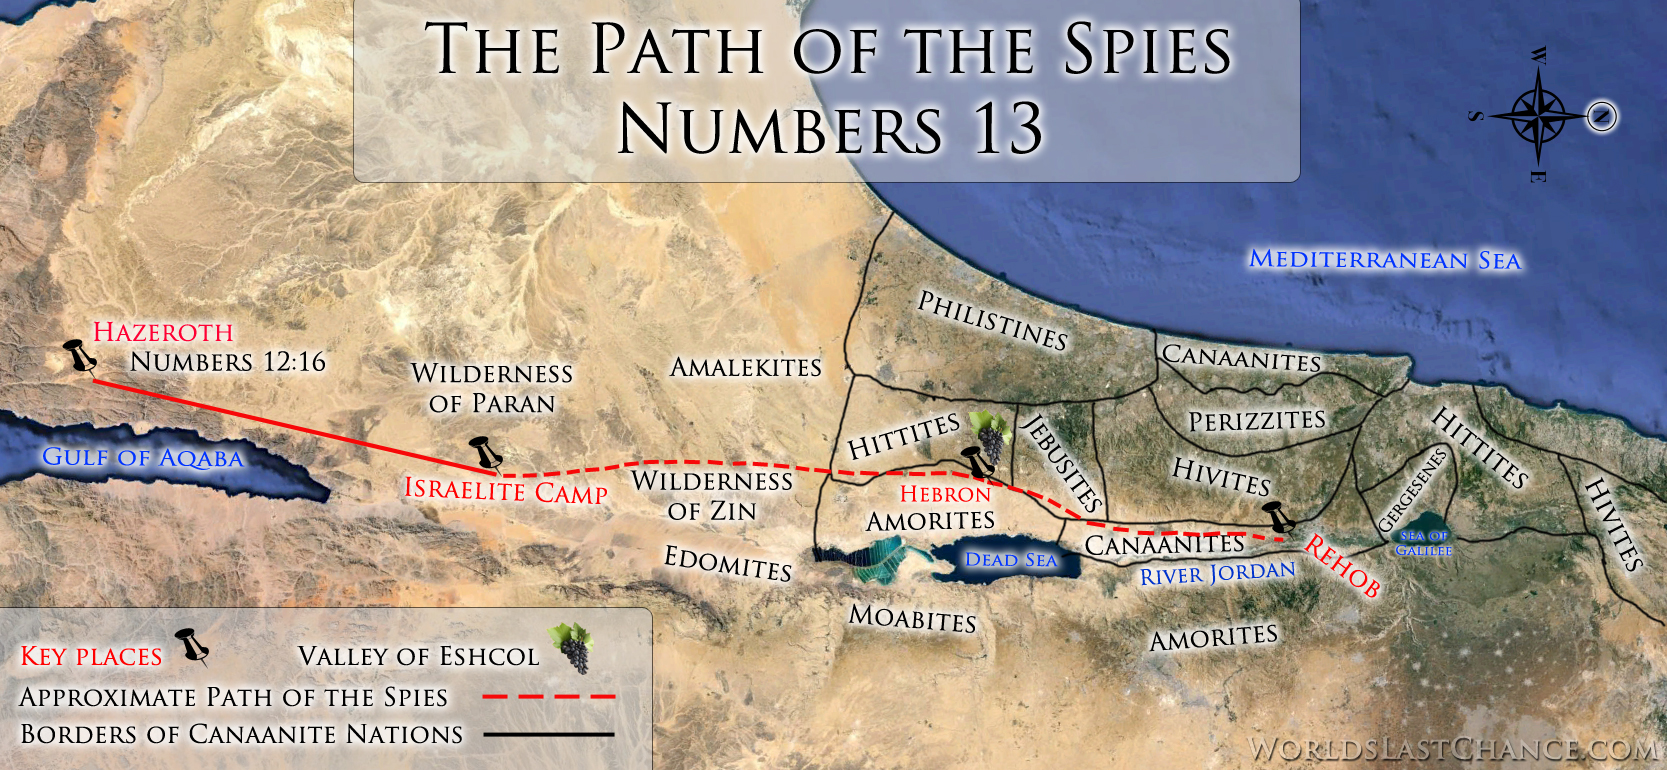
\includegraphics[width=10cm, height=10cm]{Images/PathOfTheSpies.jpg}
\caption{Suggested Route of the Hebrew Spies}
\end{figure}
\label{fig:RouteOfTheSpies}
\subsection{Numbers 13 Repeated Phrases}


%%%%%%%%%%
%%%%%%%%%%
\normalsize
 
\begin{center}
\begin{longtable}{|c|c|}
\caption[Numbers 13 Repeated Phrases]{Numbers 13 Repeated Phrases}\label{table:Repeated Phrases Numbers 13} \\
\hline \multicolumn{1}{|c|}{\textbf{Phrase}} & \multicolumn{1}{c|}{\textbf{Frequency}} \\ \hline 
\endfirsthead
 
\multicolumn{2}{c}
{{\bfseries \tablename\ \thetable{} -- continued from previous page}} \\  
\hline \multicolumn{1}{|c|}{\textbf{Phrase}} & \multicolumn{1}{c|}{\textbf{Frequency}} \\ \hline 
\endhead
 
\hline \multicolumn{2}{c}{{ }} \\ \hline
\endfoot 
of the & 17\\ \hline 
the land & 14\\ \hline 
tribe of & 14\\ \hline 
the tribe & 13\\ \hline 
the tribe of & 13\\ \hline 
the son & 13\\ \hline 
the son of & 13\\ \hline 
son of & 13\\ \hline 
Of the & 11\\ \hline 
Of the tribe & 11\\ \hline 
Of the tribe of & 11\\ \hline 
the children & 7\\ \hline 
the children of & 7\\ \hline 
children of & 7\\ \hline 
and the & 6\\ \hline 
And they & 6\\ \hline 
unto the & 5\\ \hline 
the children of Israel & 5\\ \hline 
children of Israel & 5\\ \hline 
of Israel & 5\\ \hline 
the people & 5\\ \hline 
dwell in & 5\\ \hline 
by the & 4\\ \hline 
of the land & 4\\ \hline 
that they & 3\\ \hline 
the land of & 3\\ \hline 
land of & 3\\ \hline 
And Moses & 3\\ \hline 
the wilderness & 3\\ \hline 
the wilderness of & 3\\ \hline 
wilderness of & 3\\ \hline 
and said & 3\\ \hline 
go up & 3\\ \hline 
the fruit & 3\\ \hline 
the fruit of & 3\\ \hline 
fruit of & 3\\ \hline 
came unto & 3\\ \hline 
of Anak & 3\\ \hline 
all the & 3\\ \hline 
dwell in the & 3\\ \hline 
in the & 3\\ \hline 
we saw & 3\\ \hline 
\end{longtable}
\end{center}



%%%%%%%%%%
%%%%%%%%%%



\section{Numbers 13 Word Statistics}


%%%%%%%%%%
%%%%%%%%%%
\normalsize
 
\begin{center}
\begin{longtable}{l|c|c|c|c}
\caption[Numbers 13 Statistics]{Numbers 13 Statistics}\label{table:Statistics for Numbers 13} \\
\hline \multicolumn{1}{|c|}{\textbf{Verse(s)}} & \multicolumn{1}{|c|}{\textbf{Count}} & \multicolumn{1}{|c|}{\textbf{Unique}} & \multicolumn{1}{|c|}{\textbf{Italics}} & \multicolumn{1}{|c|}{\textbf{Uniq Italic}}  \\ \hline 
\endfirsthead
 
\multicolumn{5}{c}
{{\bfseries \tablename\ \thetable{} -- continued from previous page}} \\  
\hline \multicolumn{1}{|c|}{\textbf{Verse(s)}} & \multicolumn{1}{|c|}{\textbf{Count}} & \multicolumn{1}{|c|}{\textbf{Unique}} & \multicolumn{1}{|c|}{\textbf{Italics}} & \multicolumn{1}{|c|}{\textbf{Uniq Italic}}  \\ \hline 
\endhead
 
\hline \multicolumn{5}{|r|}{{Continued if needed}} \\ \hline
\endfoot 
1 & 7 & 7 & 0 & 0\\ \hline
2 & 36 & 30 & 0 & 0\\ \hline
3 & 25 & 19 & 1 & 1\\ \hline
4 & 15 & 12 & 1 & 1\\ \hline
5 & 10 & 8 & 0 & 0\\ \hline
6 & 10 & 8 & 0 & 0\\ \hline
7 & 10 & 8 & 0 & 0\\ \hline
8 & 10 & 8 & 0 & 0\\ \hline
9 & 10 & 8 & 0 & 0\\ \hline
10 & 10 & 8 & 0 & 0\\ \hline
11 & 16 & 10 & 1 & 1\\ \hline
12 & 10 & 8 & 0 & 0\\ \hline
13 & 10 & 8 & 0 & 0\\ \hline
14 & 10 & 8 & 0 & 0\\ \hline
15 & 10 & 8 & 0 & 0\\ \hline
16 & 24 & 19 & 1 & 1\\ \hline
17 & 27 & 23 & 1 & 1\\ \hline
18 & 22 & 20 & 2 & 2\\ \hline
19 & 31 & 21 & 4 & 3\\ \hline
20 & 42 & 28 & 3 & 3\\ \hline
21 & 20 & 19 & 0 & 0\\ \hline
22 & 30 & 27 & 1 & 1\\ \hline
23 & 39 & 29 & 2 & 2\\ \hline
24 & 22 & 18 & 0 & 0\\ \hline
25 & 11 & 11 & 0 & 0\\ \hline
26 & 46 & 25 & 0 & 0\\ \hline
27 & 30 & 25 & 1 & 1\\ \hline
28 & 27 & 23 & 3 & 3\\ \hline
29 & 35 & 18 & 0 & 0\\ \hline
30 & 26 & 24 & 0 & 0\\ \hline
31 & 25 & 23 & 1 & 1\\ \hline
32 & 54 & 40 & 2 & 2\\ \hline
33 & 31 & 21 & 2 & 2\\ \hline
Total & 741 & 257 & 26 & 12
\end{longtable}
\end{center}



%%%%%%%%%%
%%%%%%%%%%


\subsection{Numbers 13 Words by Frequency}


%%%%%%%%%%
%%%%%%%%%%
\normalsize
 
\begin{center}
\begin{longtable}{l|r}
\caption[Numbers 13 Words by Frequency]{Numbers 13 Words by Frequency}\label{table:WordsbyFrequency for Numbers 13} \\
\hline \multicolumn{1}{|c|}{\textbf{Word}} & \multicolumn{1}{c|}{\textbf{Frequency}} \\ \hline 
\endfirsthead
 
\multicolumn{2}{c}
{{\bfseries \tablename\ \thetable{} -- continued from previous page}} \\  
\hline \multicolumn{1}{|c|}{\textbf{Word}} & \multicolumn{1}{c|}{\textbf{Frequency}} \\ \hline 
\endhead
 
\hline \multicolumn{2}{c}{{ }} \\ \hline
\endfoot 
the & 89\\ \hline 
of & 65\\ \hline 
and & 34\\ \hline 
And & 17\\ \hline 
land & 16\\ \hline 
they & 14\\ \hline 
tribe & 14\\ \hline 
son & 13\\ \hline 
unto & 11\\ \hline 
Of & 11\\ \hline 
in & 11\\ \hline 
to & 10\\ \hline 
it & 10\\ \hline 
that & 8\\ \hline 
up & 8\\ \hline 
we & 8\\ \hline 
Moses & 7\\ \hline 
children & 7\\ \hline 
men & 6\\ \hline 
a & 6\\ \hline 
them & 6\\ \hline 
or & 6\\ \hline 
dwell & 6\\ \hline 
which & 5\\ \hline 
Israel & 5\\ \hline 
from & 5\\ \hline 
\emph{is} & 5\\ \hline 
people & 5\\ \hline 
whether & 5\\ \hline 
\emph{be} & 5\\ \hline 
by & 4\\ \hline 
all & 4\\ \hline 
\emph{are} & 4\\ \hline 
said & 4\\ \hline 
what & 4\\ \hline 
came & 4\\ \hline 
their & 3\\ \hline 
sent & 3\\ \hline 
wilderness & 3\\ \hline 
\emph{were} & 3\\ \hline 
go & 3\\ \hline 
strong & 3\\ \hline 
there & 3\\ \hline 
be & 3\\ \hline 
fruit & 3\\ \hline 
grapes & 3\\ \hline 
went & 3\\ \hline 
Anak & 3\\ \hline 
with & 3\\ \hline 
The & 3\\ \hline 
saw & 3\\ \hline 
LORD & 2\\ \hline 
saying & 2\\ \hline 
thou & 2\\ \hline 
search & 2\\ \hline 
Canaan & 2\\ \hline 
every & 2\\ \hline 
ye & 2\\ \hline 
one & 2\\ \hline 
Paran & 2\\ \hline 
names & 2\\ \hline 
Caleb & 2\\ \hline 
Joseph & 2\\ \hline 
Oshea & 2\\ \hline 
Nun & 2\\ \hline 
spy & 2\\ \hline 
out & 2\\ \hline 
called & 2\\ \hline 
this & 2\\ \hline 
therein & 2\\ \hline 
good & 2\\ \hline 
cities & 2\\ \hline 
\emph{they} & 2\\ \hline 
not & 2\\ \hline 
Now & 2\\ \hline 
time & 2\\ \hline 
searched & 2\\ \hline 
as & 2\\ \hline 
south & 2\\ \hline 
Hebron & 2\\ \hline 
was & 2\\ \hline 
before & 2\\ \hline 
brook & 2\\ \hline 
Eshcol & 2\\ \hline 
cut & 2\\ \hline 
down & 2\\ \hline 
thence & 2\\ \hline 
cluster & 2\\ \hline 
congregation & 2\\ \hline 
brought & 2\\ \hline 
him & 2\\ \hline 
We & 2\\ \hline 
us & 2\\ \hline 
great & 2\\ \hline 
for & 2\\ \hline 
able & 2\\ \hline 
giants & 2\\ \hline 
were & 2\\ \hline 
sight & 2\\ \hline 
spake & 1\\ \hline 
Send & 1\\ \hline 
may & 1\\ \hline 
I & 1\\ \hline 
give & 1\\ \hline 
fathers & 1\\ \hline 
shall & 1\\ \hline 
send & 1\\ \hline 
man & 1\\ \hline 
ruler & 1\\ \hline 
among & 1\\ \hline 
commandment & 1\\ \hline 
those & 1\\ \hline 
heads & 1\\ \hline 
these & 1\\ \hline 
Reuben & 1\\ \hline 
Shammua & 1\\ \hline 
Zaccur & 1\\ \hline 
Simeon & 1\\ \hline 
Shaphat & 1\\ \hline 
Hori & 1\\ \hline 
Judah & 1\\ \hline 
Jephunneh & 1\\ \hline 
Issachar & 1\\ \hline 
Igal & 1\\ \hline 
Ephraim & 1\\ \hline 
Benjamin & 1\\ \hline 
Palti & 1\\ \hline 
Raphu & 1\\ \hline 
Zebulun & 1\\ \hline 
Gaddiel & 1\\ \hline 
Sodi & 1\\ \hline 
\emph{namely} & 1\\ \hline 
Manasseh & 1\\ \hline 
Gaddi & 1\\ \hline 
Susi & 1\\ \hline 
Dan & 1\\ \hline 
Ammiel & 1\\ \hline 
Gemalli & 1\\ \hline 
Asher & 1\\ \hline 
Sethur & 1\\ \hline 
Michael & 1\\ \hline 
Naphtali & 1\\ \hline 
Nahbi & 1\\ \hline 
Vophsi & 1\\ \hline 
Gad & 1\\ \hline 
Geuel & 1\\ \hline 
Machi & 1\\ \hline 
These & 1\\ \hline 
Jehoshua & 1\\ \hline 
Get & 1\\ \hline 
you & 1\\ \hline 
\emph{way} & 1\\ \hline 
southward & 1\\ \hline 
into & 1\\ \hline 
mountain & 1\\ \hline 
see & 1\\ \hline 
dwelleth & 1\\ \hline 
weak & 1\\ \hline 
few & 1\\ \hline 
many & 1\\ \hline 
bad & 1\\ \hline 
tents & 1\\ \hline 
holds & 1\\ \hline 
fat & 1\\ \hline 
lean & 1\\ \hline 
wood & 1\\ \hline 
courage & 1\\ \hline 
bring & 1\\ \hline 
\emph{was} & 1\\ \hline 
firstripe & 1\\ \hline 
So & 1\\ \hline 
Zin & 1\\ \hline 
Rehob & 1\\ \hline 
come & 1\\ \hline 
Hamath & 1\\ \hline 
ascended & 1\\ \hline 
where & 1\\ \hline 
Ahiman & 1\\ \hline 
Sheshai & 1\\ \hline 
Talmai & 1\\ \hline 
built & 1\\ \hline 
seven & 1\\ \hline 
years & 1\\ \hline 
Zoan & 1\\ \hline 
Egypt & 1\\ \hline 
branch & 1\\ \hline 
bare & 1\\ \hline 
between & 1\\ \hline 
two & 1\\ \hline 
upon & 1\\ \hline 
staff & 1\\ \hline 
\emph{brought} & 1\\ \hline 
pomegranates & 1\\ \hline 
figs & 1\\ \hline 
place & 1\\ \hline 
because & 1\\ \hline 
returned & 1\\ \hline 
searching & 1\\ \hline 
after & 1\\ \hline 
forty & 1\\ \hline 
days & 1\\ \hline 
Aaron & 1\\ \hline 
Kadesh & 1\\ \hline 
back & 1\\ \hline 
word & 1\\ \hline 
shewed & 1\\ \hline 
told & 1\\ \hline 
whither & 1\\ \hline 
sentest & 1\\ \hline 
surely & 1\\ \hline 
floweth & 1\\ \hline 
milk & 1\\ \hline 
honey & 1\\ \hline 
Nevertheless & 1\\ \hline 
walled & 1\\ \hline 
\emph{and} & 1\\ \hline 
very & 1\\ \hline 
moreover & 1\\ \hline 
Amalekites & 1\\ \hline 
Hittites & 1\\ \hline 
Jebusites & 1\\ \hline 
Amorites & 1\\ \hline 
mountains & 1\\ \hline 
Canaanites & 1\\ \hline 
sea & 1\\ \hline 
coast & 1\\ \hline 
Jordan & 1\\ \hline 
stilled & 1\\ \hline 
Let & 1\\ \hline 
at & 1\\ \hline 
once & 1\\ \hline 
possess & 1\\ \hline 
are & 1\\ \hline 
well & 1\\ \hline 
overcome & 1\\ \hline 
But & 1\\ \hline 
against & 1\\ \hline 
stronger & 1\\ \hline 
than & 1\\ \hline 
an & 1\\ \hline 
evil & 1\\ \hline 
report & 1\\ \hline 
had & 1\\ \hline 
through & 1\\ \hline 
have & 1\\ \hline 
gone & 1\\ \hline 
eateth & 1\\ \hline 
inhabitants & 1\\ \hline 
thereof & 1\\ \hline 
stature & 1\\ \hline 
sons & 1\\ \hline 
\emph{which} & 1\\ \hline 
\emph{come} & 1\\ \hline 
our & 1\\ \hline 
own & 1\\ \hline 
grasshoppers & 1\\ \hline 
so & 1\\ \hline 
\end{longtable}
\end{center}



%%%%%%%%%%
%%%%%%%%%%


\subsection{Numbers 13 Words Alphabetically}


%%%%%%%%%%
%%%%%%%%%%
\normalsize
 
\begin{center}
\begin{longtable}{l|r}
\caption[Numbers 13 Words Alphabetically]{Numbers 13 Words Alphabetically}\label{table:WordsAlphabetically for Numbers 13} \\
\hline \multicolumn{1}{|c|}{\textbf{Word}} & \multicolumn{1}{c|}{\textbf{Frequency}} \\ \hline 
\endfirsthead
 
\multicolumn{2}{c}
{{\bfseries \tablename\ \thetable{} -- continued from previous page}} \\  
\hline \multicolumn{1}{|c|}{\textbf{Word}} & \multicolumn{1}{c|}{\textbf{Frequency}} \\ \hline 
\endhead
 
\hline \multicolumn{2}{c}{{ }} \\ \hline
\endfoot 
Aaron & 1\\ \hline 
Ahiman & 1\\ \hline 
Amalekites & 1\\ \hline 
Ammiel & 1\\ \hline 
Amorites & 1\\ \hline 
Anak & 3\\ \hline 
And & 17\\ \hline 
Asher & 1\\ \hline 
Benjamin & 1\\ \hline 
But & 1\\ \hline 
Caleb & 2\\ \hline 
Canaan & 2\\ \hline 
Canaanites & 1\\ \hline 
Dan & 1\\ \hline 
Egypt & 1\\ \hline 
Ephraim & 1\\ \hline 
Eshcol & 2\\ \hline 
Gad & 1\\ \hline 
Gaddi & 1\\ \hline 
Gaddiel & 1\\ \hline 
Gemalli & 1\\ \hline 
Get & 1\\ \hline 
Geuel & 1\\ \hline 
Hamath & 1\\ \hline 
Hebron & 2\\ \hline 
Hittites & 1\\ \hline 
Hori & 1\\ \hline 
I & 1\\ \hline 
Igal & 1\\ \hline 
Israel & 5\\ \hline 
Issachar & 1\\ \hline 
Jebusites & 1\\ \hline 
Jehoshua & 1\\ \hline 
Jephunneh & 1\\ \hline 
Jordan & 1\\ \hline 
Joseph & 2\\ \hline 
Judah & 1\\ \hline 
Kadesh & 1\\ \hline 
LORD & 2\\ \hline 
Let & 1\\ \hline 
Machi & 1\\ \hline 
Manasseh & 1\\ \hline 
Michael & 1\\ \hline 
Moses & 7\\ \hline 
Nahbi & 1\\ \hline 
Naphtali & 1\\ \hline 
Nevertheless & 1\\ \hline 
Now & 2\\ \hline 
Nun & 2\\ \hline 
Of & 11\\ \hline 
Oshea & 2\\ \hline 
Palti & 1\\ \hline 
Paran & 2\\ \hline 
Raphu & 1\\ \hline 
Rehob & 1\\ \hline 
Reuben & 1\\ \hline 
Send & 1\\ \hline 
Sethur & 1\\ \hline 
Shammua & 1\\ \hline 
Shaphat & 1\\ \hline 
Sheshai & 1\\ \hline 
Simeon & 1\\ \hline 
So & 1\\ \hline 
Sodi & 1\\ \hline 
Susi & 1\\ \hline 
Talmai & 1\\ \hline 
The & 3\\ \hline 
These & 1\\ \hline 
Vophsi & 1\\ \hline 
We & 2\\ \hline 
Zaccur & 1\\ \hline 
Zebulun & 1\\ \hline 
Zin & 1\\ \hline 
Zoan & 1\\ \hline 
\emph{and} & 1\\ \hline 
\emph{are} & 4\\ \hline 
\emph{be} & 5\\ \hline 
\emph{brought} & 1\\ \hline 
\emph{come} & 1\\ \hline 
\emph{is} & 5\\ \hline 
\emph{namely} & 1\\ \hline 
\emph{they} & 2\\ \hline 
\emph{was} & 1\\ \hline 
\emph{way} & 1\\ \hline 
\emph{were} & 3\\ \hline 
\emph{which} & 1\\ \hline 
a & 6\\ \hline 
able & 2\\ \hline 
after & 1\\ \hline 
against & 1\\ \hline 
all & 4\\ \hline 
among & 1\\ \hline 
an & 1\\ \hline 
and & 34\\ \hline 
are & 1\\ \hline 
as & 2\\ \hline 
ascended & 1\\ \hline 
at & 1\\ \hline 
back & 1\\ \hline 
bad & 1\\ \hline 
bare & 1\\ \hline 
be & 3\\ \hline 
because & 1\\ \hline 
before & 2\\ \hline 
between & 1\\ \hline 
branch & 1\\ \hline 
bring & 1\\ \hline 
brook & 2\\ \hline 
brought & 2\\ \hline 
built & 1\\ \hline 
by & 4\\ \hline 
called & 2\\ \hline 
came & 4\\ \hline 
children & 7\\ \hline 
cities & 2\\ \hline 
cluster & 2\\ \hline 
coast & 1\\ \hline 
come & 1\\ \hline 
commandment & 1\\ \hline 
congregation & 2\\ \hline 
courage & 1\\ \hline 
cut & 2\\ \hline 
days & 1\\ \hline 
down & 2\\ \hline 
dwell & 6\\ \hline 
dwelleth & 1\\ \hline 
eateth & 1\\ \hline 
every & 2\\ \hline 
evil & 1\\ \hline 
fat & 1\\ \hline 
fathers & 1\\ \hline 
few & 1\\ \hline 
figs & 1\\ \hline 
firstripe & 1\\ \hline 
floweth & 1\\ \hline 
for & 2\\ \hline 
forty & 1\\ \hline 
from & 5\\ \hline 
fruit & 3\\ \hline 
giants & 2\\ \hline 
give & 1\\ \hline 
go & 3\\ \hline 
gone & 1\\ \hline 
good & 2\\ \hline 
grapes & 3\\ \hline 
grasshoppers & 1\\ \hline 
great & 2\\ \hline 
had & 1\\ \hline 
have & 1\\ \hline 
heads & 1\\ \hline 
him & 2\\ \hline 
holds & 1\\ \hline 
honey & 1\\ \hline 
in & 11\\ \hline 
inhabitants & 1\\ \hline 
into & 1\\ \hline 
it & 10\\ \hline 
land & 16\\ \hline 
lean & 1\\ \hline 
man & 1\\ \hline 
many & 1\\ \hline 
may & 1\\ \hline 
men & 6\\ \hline 
milk & 1\\ \hline 
moreover & 1\\ \hline 
mountain & 1\\ \hline 
mountains & 1\\ \hline 
names & 2\\ \hline 
not & 2\\ \hline 
of & 65\\ \hline 
once & 1\\ \hline 
one & 2\\ \hline 
or & 6\\ \hline 
our & 1\\ \hline 
out & 2\\ \hline 
overcome & 1\\ \hline 
own & 1\\ \hline 
people & 5\\ \hline 
place & 1\\ \hline 
pomegranates & 1\\ \hline 
possess & 1\\ \hline 
report & 1\\ \hline 
returned & 1\\ \hline 
ruler & 1\\ \hline 
said & 4\\ \hline 
saw & 3\\ \hline 
saying & 2\\ \hline 
sea & 1\\ \hline 
search & 2\\ \hline 
searched & 2\\ \hline 
searching & 1\\ \hline 
see & 1\\ \hline 
send & 1\\ \hline 
sent & 3\\ \hline 
sentest & 1\\ \hline 
seven & 1\\ \hline 
shall & 1\\ \hline 
shewed & 1\\ \hline 
sight & 2\\ \hline 
so & 1\\ \hline 
son & 13\\ \hline 
sons & 1\\ \hline 
south & 2\\ \hline 
southward & 1\\ \hline 
spake & 1\\ \hline 
spy & 2\\ \hline 
staff & 1\\ \hline 
stature & 1\\ \hline 
stilled & 1\\ \hline 
strong & 3\\ \hline 
stronger & 1\\ \hline 
surely & 1\\ \hline 
tents & 1\\ \hline 
than & 1\\ \hline 
that & 8\\ \hline 
the & 89\\ \hline 
their & 3\\ \hline 
them & 6\\ \hline 
thence & 2\\ \hline 
there & 3\\ \hline 
therein & 2\\ \hline 
thereof & 1\\ \hline 
these & 1\\ \hline 
they & 14\\ \hline 
this & 2\\ \hline 
those & 1\\ \hline 
thou & 2\\ \hline 
through & 1\\ \hline 
time & 2\\ \hline 
to & 10\\ \hline 
told & 1\\ \hline 
tribe & 14\\ \hline 
two & 1\\ \hline 
unto & 11\\ \hline 
up & 8\\ \hline 
upon & 1\\ \hline 
us & 2\\ \hline 
very & 1\\ \hline 
walled & 1\\ \hline 
was & 2\\ \hline 
we & 8\\ \hline 
weak & 1\\ \hline 
well & 1\\ \hline 
went & 3\\ \hline 
were & 2\\ \hline 
what & 4\\ \hline 
where & 1\\ \hline 
whether & 5\\ \hline 
which & 5\\ \hline 
whither & 1\\ \hline 
wilderness & 3\\ \hline 
with & 3\\ \hline 
wood & 1\\ \hline 
word & 1\\ \hline 
ye & 2\\ \hline 
years & 1\\ \hline 
you & 1\\ \hline 
\end{longtable}
\end{center}



%%%%%%%%%%
%%%%%%%%%%


\subsection{Numbers 13 Words by Length}


%%%%%%%%%%
%%%%%%%%%%
\normalsize
 
\begin{center}
\begin{longtable}{l|p{3.75in}}
\caption[Numbers 13 Words by Length]{Numbers 13 Words by Length}\label{table:WordsAlphabetically for Numbers 13} \\
\hline \multicolumn{1}{|c|}{\textbf{Length}} & \multicolumn{1}{c|}{\textbf{Words}} \\ \hline 
\endfirsthead
\hline \multicolumn{1}{|c|}{\textbf{Length}} & \multicolumn{1}{c|}{\textbf{Words}} \\ \hline 
\multicolumn{2}{c}
{{\bfseries \tablename\ \thetable{} -- continued from previous page}} \\  
\hline \multicolumn{1}{|c|}{\textbf{Word}} & \multicolumn{1}{c|}{\textbf{Frequency}} \\ \hline 
\endhead
 
\hline \multicolumn{2}{c}{{ }} \\ \hline
\endfoot 
1 & I, a\\ \hline 
2 & of, ye, by, Of, to, up, go, it, \emph{is}, \emph{be}, or, in, be, So, as, We, us, we, at, an, so\\ \hline 
3 & And, the, men, may, man, one, all, son, Nun, Dan, Gad, \emph{are}, spy, out, and, Get, you, \emph{way}, see, few, bad, fat, not, Now, \emph{was}, Zin, was, cut, two, The, him, \emph{and}, saw, sea, Let, for, are, But, had, our, own\\ \hline 
4 & LORD, unto, Send, thou, that, they, land, give, send, them, sent, from, \emph{were}, Hori, Igal, Sodi, Susi, said, this, into, what, weak, many, good, \emph{they}, lean, wood, time, went, come, came, Anak, Zoan, down, with, bare, upon, figs, days, back, word, told, milk, very, once, well, able, than, evil, have, gone, sons, \emph{come}, were\\ \hline 
5 & spake, Moses, which, every, tribe, their, shall, ruler, among, Paran, those, heads, these, names, Judah, Caleb, Oshea, Palti, Raphu, Gaddi, Asher, Nahbi, Geuel, Machi, These, dwell, tents, holds, there, bring, fruit, Rehob, south, where, built, seven, years, Egypt, brook, staff, place, after, forty, Aaron, honey, great, coast, \emph{which}, sight\\ \hline 
6 & saying, search, Canaan, Israel, Reuben, Zaccur, Simeon, Joseph, \emph{namely}, Ammiel, Sethur, Vophsi, called, people, strong, cities, grapes, Hamath, Hebron, Ahiman, Talmai, before, Eshcol, thence, branch, Kadesh, shewed, surely, walled, Jordan, report, eateth, giants\\ \hline 
7 & fathers, Shammua, Shaphat, Ephraim, Zebulun, Gaddiel, Gemalli, Michael, therein, whether, courage, Sheshai, cluster, between, \emph{brought}, because, brought, whither, sentest, floweth, stilled, possess, against, through, thereof, stature\\ \hline 
8 & children, Issachar, Benjamin, Manasseh, Naphtali, Jehoshua, mountain, dwelleth, searched, ascended, returned, moreover, Hittites, Amorites, overcome, stronger\\ \hline 
9 & Jephunneh, southward, firstripe, searching, Jebusites, mountains\\ \hline 
10 & wilderness, Amalekites, Canaanites\\ \hline 
11 & commandment, inhabitants\\ \hline 
12 & pomegranates, congregation, Nevertheless, grasshoppers\\ \hline 
\end{longtable}
\end{center}



%%%%%%%%%%
%%%%%%%%%%




\chapter{Numbers 14}



\marginpar{\scriptsize \centering \fcolorbox{bone}{lime}{\textbf{THE LAST STRAW}}\\ (Numbers 14:1-45) \begin{compactenum}[I.][8]
    \item \textbf{More Complaints} \index[scripture]{Numbers!Num 14:02} (Numbers 14:2) 
    \item \textbf{Murmuring Citizens} \index[scripture]{Numbers!Num 14:02} (Numbers 14:2) 
    \item \textbf{Moses (and Aaron) Contrite} \index[scripture]{Numbers!Num 14:05} (Numbers 14:5) 
    \item \textbf{Miracles \fcolorbox{bone}{bone}{not} Considered} \index[scripture]{Numbers!Num 14:23} (Numbers 14:23) 
    \item \textbf{Many Condemned} \index[scripture]{Numbers!Num 14:23} (Numbers 14:23) 
    \item \textbf{Many Carcasses} \index[scripture]{Numbers!Num 14:29}\index[scripture]{Numbers!Num 14:33} (Numbers 14:29, 33) 
    \item \textbf{Mourning Commences} \index[scripture]{Numbers!Num 14:23} (Numbers 14:23) 
    \item \textbf{Military Catastrophe} \index[scripture]{Numbers!Num 14:45} (Numbers 14:45)
\end{compactenum}}


\footnote{\textcolor[cmyk]{0.99998,1,0,0}{\hyperlink{TOC}{Return to end of Table of Contents.}}}\footnote{\href{https://audiobible.com/bible/numbers_14.html}{\textcolor[cmyk]{0.99998,1,0,0}{Numbers 14 Audio}}}\textcolor[cmyk]{0.99998,1,0,0}{And \fcolorbox{bone}{bone}{all} the congregation lifted up their voice, and cried; and the people wept \fcolorbox{bone}{bone}{that}  night.}
[2] \textcolor[cmyk]{0.99998,1,0,0}{And \fcolorbox{bone}{bone}{all} the children of Israel \fcolorbox{bone}{lime}{murmured} against Moses and against Aaron: and the whole congregation said unto them, \fcolorbox{bone}{lime}{Would God} \fcolorbox{bone}{bone}{that}  we had died in \fcolorbox{bone}{bone}{the land} of Egypt! or would God we had died in this wilderness!}
[3] \textcolor[cmyk]{0.99998,1,0,0}{And wherefore hath the LORD brought us unto this land, to fall by the sword, \fcolorbox{bone}{bone}{that}  our wives and our children should be a prey? were it \fcolorbox{bone}{bone}{not} better for us to return into Egypt?}
[4] \textcolor[cmyk]{0.99998,1,0,0}{And they said one to another, Let us make a captain, and let us return into Egypt.}
[5] \textcolor[cmyk]{0.99998,1,0,0}{Then \fcolorbox{bone}{lime}{Moses and Aaron} fell on their faces before \fcolorbox{bone}{bone}{all} the assembly of the congregation of the children of Israel.}\\
\\
\P \textcolor[cmyk]{0.99998,1,0,0}{And Joshua the son of Nun, and Caleb the son of Jephunneh, \emph{which} \emph{were} of them \fcolorbox{bone}{bone}{that}  searched \fcolorbox{bone}{bone}{the land}, rent their clothes:}
[7] \textcolor[cmyk]{0.99998,1,0,0}{And they spake unto \fcolorbox{bone}{bone}{all} the company of the children of Israel, saying, The land, which we passed through to search it, \emph{is} an exceeding good land.}
[8] \textcolor[cmyk]{0.99998,1,0,0}{If the LORD delight in us, then he \fcolorbox{bone}{bone}{will} bring us into this land, and give it us; a land which floweth with milk and honey.}
[9] \textcolor[cmyk]{0.99998,1,0,0}{Only rebel \fcolorbox{bone}{bone}{not} \fcolorbox{bone}{bone}{ye} against the LORD, neither fear \fcolorbox{bone}{bone}{ye} the people of \fcolorbox{bone}{bone}{the land}; for they \emph{are} bread for us: their defence is departed from them, and the LORD \emph{is} with us: fear them not.}
[10] \textcolor[cmyk]{0.99998,1,0,0}{But \fcolorbox{bone}{bone}{all} the congregation bade stone them with stones. And the glory of the LORD appeared in the tabernacle of the congregation before \fcolorbox{bone}{bone}{all} the children of Israel.}\\
\\
\P \textcolor[cmyk]{0.99998,1,0,0}{And the LORD said unto Moses, How long \fcolorbox{bone}{bone}{will} this people provoke me? and how long \fcolorbox{bone}{bone}{will} it be ere they believe me, for \fcolorbox{bone}{bone}{all} the signs which I have shewed among them?}
[12] \textcolor[cmyk]{0.99998,1,0,0}{I \fcolorbox{bone}{bone}{will} smite them with the pestilence, and disinherit them, and \fcolorbox{bone}{bone}{will} make of thee a greater nation and mightier than they.}\\
\\
\P \textcolor[cmyk]{0.99998,1,0,0}{And Moses said unto the LORD, Then the Egyptians shall hear \emph{it}, (for thou broughtest up this people in thy might from among them;)}
[14] \textcolor[cmyk]{0.99998,1,0,0}{And they \fcolorbox{bone}{bone}{will} tell \emph{it} to the inhabitants of this land: \emph{for} they have heard \fcolorbox{bone}{bone}{that}  thou LORD \emph{art} among this people, \fcolorbox{bone}{bone}{that}  thou LORD art seen face to face, and \emph{that} thy cloud standeth over them, and \emph{that} thou goest before them, by day time in a pillar of a cloud, and in a pillar of fire by night.}\\
\\
\P \textcolor[cmyk]{0.99998,1,0,0}{Now \emph{if} thou shalt kill \emph{all} this people as one man, then the nations which have heard the fame of thee \fcolorbox{bone}{bone}{will} speak, saying,}
[16] \textcolor[cmyk]{0.99998,1,0,0}{Because the LORD was \fcolorbox{bone}{bone}{not} able to bring this people into \fcolorbox{bone}{bone}{the land} which he sware unto them, therefore he hath slain them in the wilderness.}
[17] \textcolor[cmyk]{0.99998,1,0,0}{And now, I beseech thee, let the power of my Lord be great, according as thou hast spoken, saying,}
[18] \textcolor[cmyk]{0.99998,1,0,0}{The LORD \emph{is} \fcolorbox{bone}{MYGOLD}{longsuffering}, and of great mercy, forgiving iniquity and \fcolorbox{bone}{MYGOLD}{transgression}, and by no means clearing \emph{the} \emph{guilty}, visiting the iniquity of the fathers upon the children unto the third and fourth \emph{generation}.}
[19] \textcolor[cmyk]{0.99998,1,0,0}{Pardon, I beseech thee, the iniquity of this people according unto the greatness of thy mercy, and as thou hast forgiven this people, from Egypt even until now.}
[20] \textcolor[cmyk]{0.99998,1,0,0}{And the LORD said, I have pardoned according to thy word:}
[21] \textcolor[cmyk]{0.99998,1,0,0}{But \emph{as} truly \emph{as} I live, \fcolorbox{bone}{bone}{all} the earth shall be filled with the glory of the LORD.}
[22] \textcolor[cmyk]{0.99998,1,0,0}{Because \fcolorbox{bone}{bone}{all} those men which have seen my glory, and my miracles, which I did in Egypt and in the wilderness, and have tempted me now these ten times, and have \fcolorbox{bone}{bone}{not} hearkened to my voice;}
[23] \textcolor[cmyk]{0.99998,1,0,0}{Surely they \fcolorbox{bone}{lime}{shall \fcolorbox{bone}{bone}{not} see} \fcolorbox{bone}{bone}{the land} which I sware unto their fathers, \fcolorbox{bone}{lime}{neither shall} any of them \fcolorbox{bone}{bone}{that}  provoked me see it:}
[24] \textcolor[cmyk]{0.99998,1,0,0}{But my servant Caleb, because he had another spirit with him, and hath followed me fully, him \fcolorbox{bone}{bone}{will} I bring into \fcolorbox{bone}{bone}{the land} whereinto he went; and his seed shall possess it.}
[25] \textcolor[cmyk]{0.99998,1,0,0}{(Now the Amalekites and the Canaanites dwelt in the valley.) To morrow turn you, and get you into the wilderness by the way of the Red sea.}\\
\\
\P \textcolor[cmyk]{0.99998,1,0,0}{And the LORD spake unto Moses and unto Aaron, saying,}
[27] \textcolor[cmyk]{0.99998,1,0,0}{How long \emph{shall} \emph{I} \emph{bear} \emph{with} this evil congregation, which murmur against me? I have heard the murmurings of the children of Israel, which they murmur against me.}
[28] \textcolor[cmyk]{0.99998,1,0,0}{Say unto them, \emph{As} \emph{truly} \emph{as} I live, saith the LORD, as \fcolorbox{bone}{bone}{ye} have spoken in mine ears, so \fcolorbox{bone}{bone}{will} I do to you:}
[29] \textcolor[cmyk]{0.99998,1,0,0}{Your \fcolorbox{bone}{lime}{carcases} shall fall in this wilderness; and \fcolorbox{bone}{bone}{all} \fcolorbox{bone}{bone}{that}  were numbered of you, according to your whole number, from twenty years old and upward, which have murmured against me,}
[30] \textcolor[cmyk]{0.99998,1,0,0}{Doubtless \fcolorbox{bone}{bone}{ye} shall \fcolorbox{bone}{bone}{not} come into \fcolorbox{bone}{bone}{the land}, \emph{concerning} which I sware to make you dwell therein, save Caleb the son of Jephunneh, and Joshua the son of Nun.}
[31] \textcolor[cmyk]{0.99998,1,0,0}{But your little ones, which \fcolorbox{bone}{bone}{ye} said should be a prey, them \fcolorbox{bone}{bone}{will} I bring in, and they shall know \fcolorbox{bone}{bone}{the land} which \fcolorbox{bone}{bone}{ye} have despised.}
[32] \textcolor[cmyk]{0.99998,1,0,0}{But \emph{as} \emph{for} you, your carcases, they shall fall in this wilderness.}
[33] \textcolor[cmyk]{0.99998,1,0,0}{And your children shall wander in the wilderness forty years, and bear your whoredoms, until your carcases be wasted in the wilderness.}
[34] \textcolor[cmyk]{0.99998,1,0,0}{After the number of the days in which \fcolorbox{bone}{bone}{ye} searched \fcolorbox{bone}{bone}{the land}, \emph{even} forty days, each day for a year, shall \fcolorbox{bone}{bone}{ye} bear your iniquities, \emph{even} forty years, and \fcolorbox{bone}{bone}{ye} shall know my breach of promise.}
[35] \textcolor[cmyk]{0.99998,1,0,0}{I the LORD have said, I \fcolorbox{bone}{bone}{will} surely do it unto \fcolorbox{bone}{bone}{all} this evil congregation, \fcolorbox{bone}{bone}{that}  are gathered together against me: in this wilderness they shall be consumed, and there they shall die.}
[36] \textcolor[cmyk]{0.99998,1,0,0}{And the men, which Moses sent to search \fcolorbox{bone}{bone}{the land}, who returned, and made \fcolorbox{bone}{bone}{all} the congregation to murmur against him, by bringing up a slander upon \fcolorbox{bone}{bone}{the land},}
[37] \textcolor[cmyk]{0.99998,1,0,0}{Even those men \fcolorbox{bone}{bone}{that}  did bring up the evil report upon \fcolorbox{bone}{bone}{the land}, died by the plague before the LORD.}
[38] \textcolor[cmyk]{0.99998,1,0,0}{But Joshua the son of Nun, and Caleb the son of Jephunneh, \emph{which} \emph{were} of the men \fcolorbox{bone}{bone}{that}  went to search \fcolorbox{bone}{bone}{the land}, lived \emph{still}.}
[39] \textcolor[cmyk]{0.99998,1,0,0}{And Moses told these sayings unto \fcolorbox{bone}{bone}{all} the children of Israel: and the people mourned greatly.}
[40] \textcolor[cmyk]{0.99998,1,0,0}{And they rose up early in the morning, and gat them up into the top of the mountain, saying, Lo, we \emph{be} \emph{here}, and \fcolorbox{bone}{bone}{will} go up unto the place which the LORD hath promised: for we have sinned.}\\
\\
\P \textcolor[cmyk]{0.99998,1,0,0}{And Moses said, Wherefore now do \fcolorbox{bone}{bone}{ye} transgress the commandment of the LORD? but it shall \fcolorbox{bone}{bone}{not} prosper.}
[42] \textcolor[cmyk]{0.99998,1,0,0}{Go \fcolorbox{bone}{bone}{not} up, for the LORD \emph{is} \fcolorbox{bone}{bone}{not} among you; \fcolorbox{bone}{bone}{that}  \fcolorbox{bone}{bone}{ye} be \fcolorbox{bone}{bone}{not} smitten before your enemies.}
[43] \textcolor[cmyk]{0.99998,1,0,0}{For the Amalekites and the Canaanites \emph{are} there before you, and \fcolorbox{bone}{bone}{ye} shall fall by the sword: because \fcolorbox{bone}{bone}{ye} are turned away from the LORD, therefore the LORD \fcolorbox{bone}{bone}{will} \fcolorbox{bone}{bone}{not} be with you.}
[44] \textcolor[cmyk]{0.99998,1,0,0}{But they presumed to go up unto the hill top: nevertheless the ark of the covenant of the LORD, and Moses, departed \fcolorbox{bone}{bone}{not} out of the camp.}
[45] \textcolor[cmyk]{0.99998,1,0,0}{Then the Amalekites came down, and the Canaanites which dwelt in \fcolorbox{bone}{bone}{that}  hill, and \fcolorbox{bone}{lime}{smote them}, and discomfited them, \emph{even} unto Hormah.}
\index[NWIV]{16!Numbers!Num 14:1}\index[AWIP]{And!Numbers!Num 14:1}\index[AWIP]{all!Numbers!Num 14:1}\index[AWIP]{the!Numbers!Num 14:1}\index[AWIP]{the!Numbers!Num 14:1 (2)}\index[AWIP]{congregation!Numbers!Num 14:1}\index[AWIP]{lifted!Numbers!Num 14:1}\index[AWIP]{up!Numbers!Num 14:1}\index[AWIP]{their!Numbers!Num 14:1}\index[AWIP]{voice!Numbers!Num 14:1}\index[AWIP]{and!Numbers!Num 14:1}\index[AWIP]{and!Numbers!Num 14:1 (2)}\index[AWIP]{cried!Numbers!Num 14:1}\index[AWIP]{people!Numbers!Num 14:1}\index[AWIP]{wept!Numbers!Num 14:1}\index[AWIP]{that!Numbers!Num 14:1}\index[AWIP]{night!Numbers!Num 14:1}

\index[NWIV]{39!Numbers!Num 14:2}\index[AWIP]{And!Numbers!Num 14:2}\index[AWIP]{all!Numbers!Num 14:2}\index[AWIP]{the!Numbers!Num 14:2}\index[AWIP]{the!Numbers!Num 14:2 (2)}\index[AWIP]{the!Numbers!Num 14:2 (3)}\index[AWIP]{children!Numbers!Num 14:2}\index[AWIP]{of!Numbers!Num 14:2}\index[AWIP]{of!Numbers!Num 14:2 (2)}\index[AWIP]{Israel!Numbers!Num 14:2}\index[AWIP]{murmured!Numbers!Num 14:2}\index[AWIP]{against!Numbers!Num 14:2}\index[AWIP]{against!Numbers!Num 14:2 (2)}\index[AWIP]{Moses!Numbers!Num 14:2}\index[AWIP]{and!Numbers!Num 14:2}\index[AWIP]{and!Numbers!Num 14:2 (2)}\index[AWIP]{Aaron!Numbers!Num 14:2}\index[AWIP]{whole!Numbers!Num 14:2}\index[AWIP]{congregation!Numbers!Num 14:2}\index[AWIP]{said!Numbers!Num 14:2}\index[AWIP]{unto!Numbers!Num 14:2}\index[AWIP]{them!Numbers!Num 14:2}\index[AWIP]{Would!Numbers!Num 14:2}\index[AWIP]{God!Numbers!Num 14:2}\index[AWIP]{God!Numbers!Num 14:2 (2)}\index[AWIP]{that!Numbers!Num 14:2}\index[AWIP]{we!Numbers!Num 14:2}\index[AWIP]{we!Numbers!Num 14:2 (2)}\index[AWIP]{had!Numbers!Num 14:2}\index[AWIP]{had!Numbers!Num 14:2 (2)}\index[AWIP]{died!Numbers!Num 14:2}\index[AWIP]{died!Numbers!Num 14:2 (2)}\index[AWIP]{in!Numbers!Num 14:2}\index[AWIP]{in!Numbers!Num 14:2 (2)}\index[AWIP]{land!Numbers!Num 14:2}\index[AWIP]{Egypt!Numbers!Num 14:2}\index[AWIP]{or!Numbers!Num 14:2}\index[AWIP]{would!Numbers!Num 14:2}\index[AWIP]{this!Numbers!Num 14:2}\index[AWIP]{wilderness!Numbers!Num 14:2}

\index[NWIV]{35!Numbers!Num 14:3}\index[AWIP]{And!Numbers!Num 14:3}\index[AWIP]{wherefore!Numbers!Num 14:3}\index[AWIP]{hath!Numbers!Num 14:3}\index[AWIP]{the!Numbers!Num 14:3}\index[AWIP]{the!Numbers!Num 14:3 (2)}\index[AWIP]{LORD!Numbers!Num 14:3}\index[AWIP]{brought!Numbers!Num 14:3}\index[AWIP]{us!Numbers!Num 14:3}\index[AWIP]{us!Numbers!Num 14:3 (2)}\index[AWIP]{unto!Numbers!Num 14:3}\index[AWIP]{this!Numbers!Num 14:3}\index[AWIP]{land!Numbers!Num 14:3}\index[AWIP]{to!Numbers!Num 14:3}\index[AWIP]{to!Numbers!Num 14:3 (2)}\index[AWIP]{fall!Numbers!Num 14:3}\index[AWIP]{by!Numbers!Num 14:3}\index[AWIP]{sword!Numbers!Num 14:3}\index[AWIP]{that!Numbers!Num 14:3}\index[AWIP]{our!Numbers!Num 14:3}\index[AWIP]{our!Numbers!Num 14:3 (2)}\index[AWIP]{wives!Numbers!Num 14:3}\index[AWIP]{and!Numbers!Num 14:3}\index[AWIP]{children!Numbers!Num 14:3}\index[AWIP]{should!Numbers!Num 14:3}\index[AWIP]{be!Numbers!Num 14:3}\index[AWIP]{a!Numbers!Num 14:3}\index[AWIP]{prey!Numbers!Num 14:3}\index[AWIP]{were!Numbers!Num 14:3}\index[AWIP]{it!Numbers!Num 14:3}\index[AWIP]{not!Numbers!Num 14:3}\index[AWIP]{better!Numbers!Num 14:3}\index[AWIP]{for!Numbers!Num 14:3}\index[AWIP]{return!Numbers!Num 14:3}\index[AWIP]{into!Numbers!Num 14:3}\index[AWIP]{Egypt!Numbers!Num 14:3}

\index[NWIV]{17!Numbers!Num 14:4}\index[AWIP]{And!Numbers!Num 14:4}\index[AWIP]{they!Numbers!Num 14:4}\index[AWIP]{said!Numbers!Num 14:4}\index[AWIP]{one!Numbers!Num 14:4}\index[AWIP]{to!Numbers!Num 14:4}\index[AWIP]{another!Numbers!Num 14:4}\index[AWIP]{Let!Numbers!Num 14:4}\index[AWIP]{us!Numbers!Num 14:4}\index[AWIP]{us!Numbers!Num 14:4 (2)}\index[AWIP]{make!Numbers!Num 14:4}\index[AWIP]{a!Numbers!Num 14:4}\index[AWIP]{captain!Numbers!Num 14:4}\index[AWIP]{and!Numbers!Num 14:4}\index[AWIP]{let!Numbers!Num 14:4}\index[AWIP]{return!Numbers!Num 14:4}\index[AWIP]{into!Numbers!Num 14:4}\index[AWIP]{Egypt!Numbers!Num 14:4}

\index[NWIV]{20!Numbers!Num 14:5}\index[AWIP]{Then!Numbers!Num 14:5}\index[AWIP]{Moses!Numbers!Num 14:5}\index[AWIP]{and!Numbers!Num 14:5}\index[AWIP]{Aaron!Numbers!Num 14:5}\index[AWIP]{fell!Numbers!Num 14:5}\index[AWIP]{on!Numbers!Num 14:5}\index[AWIP]{their!Numbers!Num 14:5}\index[AWIP]{faces!Numbers!Num 14:5}\index[AWIP]{before!Numbers!Num 14:5}\index[AWIP]{all!Numbers!Num 14:5}\index[AWIP]{the!Numbers!Num 14:5}\index[AWIP]{the!Numbers!Num 14:5 (2)}\index[AWIP]{the!Numbers!Num 14:5 (3)}\index[AWIP]{assembly!Numbers!Num 14:5}\index[AWIP]{of!Numbers!Num 14:5}\index[AWIP]{of!Numbers!Num 14:5 (2)}\index[AWIP]{of!Numbers!Num 14:5 (3)}\index[AWIP]{congregation!Numbers!Num 14:5}\index[AWIP]{children!Numbers!Num 14:5}\index[AWIP]{Israel!Numbers!Num 14:5}

\index[NWIV]{23!Numbers!Num 14:6}\index[AWIP]{And!Numbers!Num 14:6}\index[AWIP]{Joshua!Numbers!Num 14:6}\index[AWIP]{the!Numbers!Num 14:6}\index[AWIP]{the!Numbers!Num 14:6 (2)}\index[AWIP]{the!Numbers!Num 14:6 (3)}\index[AWIP]{son!Numbers!Num 14:6}\index[AWIP]{son!Numbers!Num 14:6 (2)}\index[AWIP]{of!Numbers!Num 14:6}\index[AWIP]{of!Numbers!Num 14:6 (2)}\index[AWIP]{of!Numbers!Num 14:6 (3)}\index[AWIP]{Nun!Numbers!Num 14:6}\index[AWIP]{and!Numbers!Num 14:6}\index[AWIP]{Caleb!Numbers!Num 14:6}\index[AWIP]{Jephunneh!Numbers!Num 14:6}\index[AWIP]{\emph{which}!Numbers!Num 14:6}\index[AWIP]{\emph{were}!Numbers!Num 14:6}\index[AWIP]{them!Numbers!Num 14:6}\index[AWIP]{that!Numbers!Num 14:6}\index[AWIP]{searched!Numbers!Num 14:6}\index[AWIP]{land!Numbers!Num 14:6}\index[AWIP]{rent!Numbers!Num 14:6}\index[AWIP]{their!Numbers!Num 14:6}\index[AWIP]{clothes!Numbers!Num 14:6}\index[AWIP]{\emph{which}!Numbers!Num 14:6}\index[AWIP]{\emph{were}!Numbers!Num 14:6}

\index[NWIV]{27!Numbers!Num 14:7}\index[AWIP]{And!Numbers!Num 14:7}\index[AWIP]{they!Numbers!Num 14:7}\index[AWIP]{spake!Numbers!Num 14:7}\index[AWIP]{unto!Numbers!Num 14:7}\index[AWIP]{all!Numbers!Num 14:7}\index[AWIP]{the!Numbers!Num 14:7}\index[AWIP]{the!Numbers!Num 14:7 (2)}\index[AWIP]{company!Numbers!Num 14:7}\index[AWIP]{of!Numbers!Num 14:7}\index[AWIP]{of!Numbers!Num 14:7 (2)}\index[AWIP]{children!Numbers!Num 14:7}\index[AWIP]{Israel!Numbers!Num 14:7}\index[AWIP]{saying!Numbers!Num 14:7}\index[AWIP]{The!Numbers!Num 14:7}\index[AWIP]{land!Numbers!Num 14:7}\index[AWIP]{land!Numbers!Num 14:7 (2)}\index[AWIP]{which!Numbers!Num 14:7}\index[AWIP]{we!Numbers!Num 14:7}\index[AWIP]{passed!Numbers!Num 14:7}\index[AWIP]{through!Numbers!Num 14:7}\index[AWIP]{to!Numbers!Num 14:7}\index[AWIP]{search!Numbers!Num 14:7}\index[AWIP]{it!Numbers!Num 14:7}\index[AWIP]{\emph{is}!Numbers!Num 14:7}\index[AWIP]{an!Numbers!Num 14:7}\index[AWIP]{exceeding!Numbers!Num 14:7}\index[AWIP]{good!Numbers!Num 14:7}\index[AWIP]{\emph{is}!Numbers!Num 14:7}

\index[NWIV]{26!Numbers!Num 14:8}\index[AWIP]{If!Numbers!Num 14:8}\index[AWIP]{the!Numbers!Num 14:8}\index[AWIP]{LORD!Numbers!Num 14:8}\index[AWIP]{delight!Numbers!Num 14:8}\index[AWIP]{in!Numbers!Num 14:8}\index[AWIP]{us!Numbers!Num 14:8}\index[AWIP]{us!Numbers!Num 14:8 (2)}\index[AWIP]{us!Numbers!Num 14:8 (3)}\index[AWIP]{then!Numbers!Num 14:8}\index[AWIP]{he!Numbers!Num 14:8}\index[AWIP]{will!Numbers!Num 14:8}\index[AWIP]{bring!Numbers!Num 14:8}\index[AWIP]{into!Numbers!Num 14:8}\index[AWIP]{this!Numbers!Num 14:8}\index[AWIP]{land!Numbers!Num 14:8}\index[AWIP]{land!Numbers!Num 14:8 (2)}\index[AWIP]{and!Numbers!Num 14:8}\index[AWIP]{and!Numbers!Num 14:8 (2)}\index[AWIP]{give!Numbers!Num 14:8}\index[AWIP]{it!Numbers!Num 14:8}\index[AWIP]{a!Numbers!Num 14:8}\index[AWIP]{which!Numbers!Num 14:8}\index[AWIP]{floweth!Numbers!Num 14:8}\index[AWIP]{with!Numbers!Num 14:8}\index[AWIP]{milk!Numbers!Num 14:8}\index[AWIP]{honey!Numbers!Num 14:8}

\index[NWIV]{36!Numbers!Num 14:9}\index[AWIP]{Only!Numbers!Num 14:9}\index[AWIP]{rebel!Numbers!Num 14:9}\index[AWIP]{not!Numbers!Num 14:9}\index[AWIP]{not!Numbers!Num 14:9 (2)}\index[AWIP]{ye!Numbers!Num 14:9}\index[AWIP]{ye!Numbers!Num 14:9 (2)}\index[AWIP]{against!Numbers!Num 14:9}\index[AWIP]{the!Numbers!Num 14:9}\index[AWIP]{the!Numbers!Num 14:9 (2)}\index[AWIP]{the!Numbers!Num 14:9 (3)}\index[AWIP]{the!Numbers!Num 14:9 (4)}\index[AWIP]{LORD!Numbers!Num 14:9}\index[AWIP]{LORD!Numbers!Num 14:9 (2)}\index[AWIP]{neither!Numbers!Num 14:9}\index[AWIP]{fear!Numbers!Num 14:9}\index[AWIP]{fear!Numbers!Num 14:9 (2)}\index[AWIP]{people!Numbers!Num 14:9}\index[AWIP]{of!Numbers!Num 14:9}\index[AWIP]{land!Numbers!Num 14:9}\index[AWIP]{for!Numbers!Num 14:9}\index[AWIP]{for!Numbers!Num 14:9 (2)}\index[AWIP]{they!Numbers!Num 14:9}\index[AWIP]{\emph{are}!Numbers!Num 14:9}\index[AWIP]{bread!Numbers!Num 14:9}\index[AWIP]{us!Numbers!Num 14:9}\index[AWIP]{us!Numbers!Num 14:9 (2)}\index[AWIP]{their!Numbers!Num 14:9}\index[AWIP]{defence!Numbers!Num 14:9}\index[AWIP]{is!Numbers!Num 14:9}\index[AWIP]{departed!Numbers!Num 14:9}\index[AWIP]{from!Numbers!Num 14:9}\index[AWIP]{them!Numbers!Num 14:9}\index[AWIP]{them!Numbers!Num 14:9 (2)}\index[AWIP]{and!Numbers!Num 14:9}\index[AWIP]{\emph{is}!Numbers!Num 14:9}\index[AWIP]{with!Numbers!Num 14:9}\index[AWIP]{\emph{are}!Numbers!Num 14:9}\index[AWIP]{\emph{is}!Numbers!Num 14:9}

\index[NWIV]{28!Numbers!Num 14:10}\index[AWIP]{But!Numbers!Num 14:10}\index[AWIP]{all!Numbers!Num 14:10}\index[AWIP]{all!Numbers!Num 14:10 (2)}\index[AWIP]{the!Numbers!Num 14:10}\index[AWIP]{the!Numbers!Num 14:10 (2)}\index[AWIP]{the!Numbers!Num 14:10 (3)}\index[AWIP]{the!Numbers!Num 14:10 (4)}\index[AWIP]{the!Numbers!Num 14:10 (5)}\index[AWIP]{the!Numbers!Num 14:10 (6)}\index[AWIP]{congregation!Numbers!Num 14:10}\index[AWIP]{congregation!Numbers!Num 14:10 (2)}\index[AWIP]{bade!Numbers!Num 14:10}\index[AWIP]{stone!Numbers!Num 14:10}\index[AWIP]{them!Numbers!Num 14:10}\index[AWIP]{with!Numbers!Num 14:10}\index[AWIP]{stones!Numbers!Num 14:10}\index[AWIP]{And!Numbers!Num 14:10}\index[AWIP]{glory!Numbers!Num 14:10}\index[AWIP]{of!Numbers!Num 14:10}\index[AWIP]{of!Numbers!Num 14:10 (2)}\index[AWIP]{of!Numbers!Num 14:10 (3)}\index[AWIP]{LORD!Numbers!Num 14:10}\index[AWIP]{appeared!Numbers!Num 14:10}\index[AWIP]{in!Numbers!Num 14:10}\index[AWIP]{tabernacle!Numbers!Num 14:10}\index[AWIP]{before!Numbers!Num 14:10}\index[AWIP]{children!Numbers!Num 14:10}\index[AWIP]{Israel!Numbers!Num 14:10}

\index[NWIV]{33!Numbers!Num 14:11}\index[AWIP]{And!Numbers!Num 14:11}\index[AWIP]{the!Numbers!Num 14:11}\index[AWIP]{the!Numbers!Num 14:11 (2)}\index[AWIP]{LORD!Numbers!Num 14:11}\index[AWIP]{said!Numbers!Num 14:11}\index[AWIP]{unto!Numbers!Num 14:11}\index[AWIP]{Moses!Numbers!Num 14:11}\index[AWIP]{How!Numbers!Num 14:11}\index[AWIP]{long!Numbers!Num 14:11}\index[AWIP]{long!Numbers!Num 14:11 (2)}\index[AWIP]{will!Numbers!Num 14:11}\index[AWIP]{will!Numbers!Num 14:11 (2)}\index[AWIP]{this!Numbers!Num 14:11}\index[AWIP]{people!Numbers!Num 14:11}\index[AWIP]{provoke!Numbers!Num 14:11}\index[AWIP]{me!Numbers!Num 14:11}\index[AWIP]{me!Numbers!Num 14:11 (2)}\index[AWIP]{and!Numbers!Num 14:11}\index[AWIP]{how!Numbers!Num 14:11}\index[AWIP]{it!Numbers!Num 14:11}\index[AWIP]{be!Numbers!Num 14:11}\index[AWIP]{ere!Numbers!Num 14:11}\index[AWIP]{they!Numbers!Num 14:11}\index[AWIP]{believe!Numbers!Num 14:11}\index[AWIP]{for!Numbers!Num 14:11}\index[AWIP]{all!Numbers!Num 14:11}\index[AWIP]{signs!Numbers!Num 14:11}\index[AWIP]{which!Numbers!Num 14:11}\index[AWIP]{I!Numbers!Num 14:11}\index[AWIP]{have!Numbers!Num 14:11}\index[AWIP]{shewed!Numbers!Num 14:11}\index[AWIP]{among!Numbers!Num 14:11}\index[AWIP]{them!Numbers!Num 14:11}

\index[NWIV]{22!Numbers!Num 14:12}\index[AWIP]{I!Numbers!Num 14:12}\index[AWIP]{will!Numbers!Num 14:12}\index[AWIP]{will!Numbers!Num 14:12 (2)}\index[AWIP]{smite!Numbers!Num 14:12}\index[AWIP]{them!Numbers!Num 14:12}\index[AWIP]{them!Numbers!Num 14:12 (2)}\index[AWIP]{with!Numbers!Num 14:12}\index[AWIP]{the!Numbers!Num 14:12}\index[AWIP]{pestilence!Numbers!Num 14:12}\index[AWIP]{and!Numbers!Num 14:12}\index[AWIP]{and!Numbers!Num 14:12 (2)}\index[AWIP]{and!Numbers!Num 14:12 (3)}\index[AWIP]{disinherit!Numbers!Num 14:12}\index[AWIP]{make!Numbers!Num 14:12}\index[AWIP]{of!Numbers!Num 14:12}\index[AWIP]{thee!Numbers!Num 14:12}\index[AWIP]{a!Numbers!Num 14:12}\index[AWIP]{greater!Numbers!Num 14:12}\index[AWIP]{nation!Numbers!Num 14:12}\index[AWIP]{mightier!Numbers!Num 14:12}\index[AWIP]{than!Numbers!Num 14:12}\index[AWIP]{they!Numbers!Num 14:12}

\index[NWIV]{24!Numbers!Num 14:13}\index[AWIP]{And!Numbers!Num 14:13}\index[AWIP]{Moses!Numbers!Num 14:13}\index[AWIP]{said!Numbers!Num 14:13}\index[AWIP]{unto!Numbers!Num 14:13}\index[AWIP]{the!Numbers!Num 14:13}\index[AWIP]{the!Numbers!Num 14:13 (2)}\index[AWIP]{LORD!Numbers!Num 14:13}\index[AWIP]{Then!Numbers!Num 14:13}\index[AWIP]{Egyptians!Numbers!Num 14:13}\index[AWIP]{shall!Numbers!Num 14:13}\index[AWIP]{hear!Numbers!Num 14:13}\index[AWIP]{\emph{it}!Numbers!Num 14:13}\index[AWIP]{(for!Numbers!Num 14:13}\index[AWIP]{thou!Numbers!Num 14:13}\index[AWIP]{broughtest!Numbers!Num 14:13}\index[AWIP]{up!Numbers!Num 14:13}\index[AWIP]{this!Numbers!Num 14:13}\index[AWIP]{people!Numbers!Num 14:13}\index[AWIP]{in!Numbers!Num 14:13}\index[AWIP]{thy!Numbers!Num 14:13}\index[AWIP]{might!Numbers!Num 14:13}\index[AWIP]{from!Numbers!Num 14:13}\index[AWIP]{among!Numbers!Num 14:13}\index[AWIP]{them)!Numbers!Num 14:13}\index[AWIP]{\emph{it}!Numbers!Num 14:13}

\index[NWIV]{60!Numbers!Num 14:14}\index[AWIP]{And!Numbers!Num 14:14}\index[AWIP]{they!Numbers!Num 14:14}\index[AWIP]{they!Numbers!Num 14:14 (2)}\index[AWIP]{will!Numbers!Num 14:14}\index[AWIP]{tell!Numbers!Num 14:14}\index[AWIP]{\emph{it}!Numbers!Num 14:14}\index[AWIP]{to!Numbers!Num 14:14}\index[AWIP]{to!Numbers!Num 14:14 (2)}\index[AWIP]{the!Numbers!Num 14:14}\index[AWIP]{inhabitants!Numbers!Num 14:14}\index[AWIP]{of!Numbers!Num 14:14}\index[AWIP]{of!Numbers!Num 14:14 (2)}\index[AWIP]{of!Numbers!Num 14:14 (3)}\index[AWIP]{this!Numbers!Num 14:14}\index[AWIP]{this!Numbers!Num 14:14 (2)}\index[AWIP]{land!Numbers!Num 14:14}\index[AWIP]{\emph{for}!Numbers!Num 14:14}\index[AWIP]{have!Numbers!Num 14:14}\index[AWIP]{heard!Numbers!Num 14:14}\index[AWIP]{that!Numbers!Num 14:14}\index[AWIP]{that!Numbers!Num 14:14 (2)}\index[AWIP]{thou!Numbers!Num 14:14}\index[AWIP]{thou!Numbers!Num 14:14 (2)}\index[AWIP]{thou!Numbers!Num 14:14 (3)}\index[AWIP]{LORD!Numbers!Num 14:14}\index[AWIP]{LORD!Numbers!Num 14:14 (2)}\index[AWIP]{\emph{art}!Numbers!Num 14:14}\index[AWIP]{among!Numbers!Num 14:14}\index[AWIP]{people!Numbers!Num 14:14}\index[AWIP]{art!Numbers!Num 14:14}\index[AWIP]{seen!Numbers!Num 14:14}\index[AWIP]{face!Numbers!Num 14:14}\index[AWIP]{face!Numbers!Num 14:14 (2)}\index[AWIP]{and!Numbers!Num 14:14}\index[AWIP]{and!Numbers!Num 14:14 (2)}\index[AWIP]{and!Numbers!Num 14:14 (3)}\index[AWIP]{\emph{that}!Numbers!Num 14:14}\index[AWIP]{\emph{that}!Numbers!Num 14:14 (2)}\index[AWIP]{thy!Numbers!Num 14:14}\index[AWIP]{cloud!Numbers!Num 14:14}\index[AWIP]{cloud!Numbers!Num 14:14 (2)}\index[AWIP]{standeth!Numbers!Num 14:14}\index[AWIP]{over!Numbers!Num 14:14}\index[AWIP]{them!Numbers!Num 14:14}\index[AWIP]{them!Numbers!Num 14:14 (2)}\index[AWIP]{goest!Numbers!Num 14:14}\index[AWIP]{before!Numbers!Num 14:14}\index[AWIP]{by!Numbers!Num 14:14}\index[AWIP]{by!Numbers!Num 14:14 (2)}\index[AWIP]{day!Numbers!Num 14:14}\index[AWIP]{time!Numbers!Num 14:14}\index[AWIP]{in!Numbers!Num 14:14}\index[AWIP]{in!Numbers!Num 14:14 (2)}\index[AWIP]{a!Numbers!Num 14:14}\index[AWIP]{a!Numbers!Num 14:14 (2)}\index[AWIP]{a!Numbers!Num 14:14 (3)}\index[AWIP]{pillar!Numbers!Num 14:14}\index[AWIP]{pillar!Numbers!Num 14:14 (2)}\index[AWIP]{fire!Numbers!Num 14:14}\index[AWIP]{night!Numbers!Num 14:14}\index[AWIP]{\emph{it}!Numbers!Num 14:14}\index[AWIP]{\emph{for}!Numbers!Num 14:14}\index[AWIP]{\emph{art}!Numbers!Num 14:14}\index[AWIP]{\emph{that}!Numbers!Num 14:14}\index[AWIP]{\emph{that}!Numbers!Num 14:14 (2)}

\index[NWIV]{24!Numbers!Num 14:15}\index[AWIP]{Now!Numbers!Num 14:15}\index[AWIP]{\emph{if}!Numbers!Num 14:15}\index[AWIP]{thou!Numbers!Num 14:15}\index[AWIP]{shalt!Numbers!Num 14:15}\index[AWIP]{kill!Numbers!Num 14:15}\index[AWIP]{\emph{all}!Numbers!Num 14:15}\index[AWIP]{this!Numbers!Num 14:15}\index[AWIP]{people!Numbers!Num 14:15}\index[AWIP]{as!Numbers!Num 14:15}\index[AWIP]{one!Numbers!Num 14:15}\index[AWIP]{man!Numbers!Num 14:15}\index[AWIP]{then!Numbers!Num 14:15}\index[AWIP]{the!Numbers!Num 14:15}\index[AWIP]{the!Numbers!Num 14:15 (2)}\index[AWIP]{nations!Numbers!Num 14:15}\index[AWIP]{which!Numbers!Num 14:15}\index[AWIP]{have!Numbers!Num 14:15}\index[AWIP]{heard!Numbers!Num 14:15}\index[AWIP]{fame!Numbers!Num 14:15}\index[AWIP]{of!Numbers!Num 14:15}\index[AWIP]{thee!Numbers!Num 14:15}\index[AWIP]{will!Numbers!Num 14:15}\index[AWIP]{speak!Numbers!Num 14:15}\index[AWIP]{saying!Numbers!Num 14:15}\index[AWIP]{\emph{if}!Numbers!Num 14:15}\index[AWIP]{\emph{all}!Numbers!Num 14:15}

\index[NWIV]{26!Numbers!Num 14:16}\index[AWIP]{Because!Numbers!Num 14:16}\index[AWIP]{the!Numbers!Num 14:16}\index[AWIP]{the!Numbers!Num 14:16 (2)}\index[AWIP]{the!Numbers!Num 14:16 (3)}\index[AWIP]{LORD!Numbers!Num 14:16}\index[AWIP]{was!Numbers!Num 14:16}\index[AWIP]{not!Numbers!Num 14:16}\index[AWIP]{able!Numbers!Num 14:16}\index[AWIP]{to!Numbers!Num 14:16}\index[AWIP]{bring!Numbers!Num 14:16}\index[AWIP]{this!Numbers!Num 14:16}\index[AWIP]{people!Numbers!Num 14:16}\index[AWIP]{into!Numbers!Num 14:16}\index[AWIP]{land!Numbers!Num 14:16}\index[AWIP]{which!Numbers!Num 14:16}\index[AWIP]{he!Numbers!Num 14:16}\index[AWIP]{he!Numbers!Num 14:16 (2)}\index[AWIP]{sware!Numbers!Num 14:16}\index[AWIP]{unto!Numbers!Num 14:16}\index[AWIP]{them!Numbers!Num 14:16}\index[AWIP]{them!Numbers!Num 14:16 (2)}\index[AWIP]{therefore!Numbers!Num 14:16}\index[AWIP]{hath!Numbers!Num 14:16}\index[AWIP]{slain!Numbers!Num 14:16}\index[AWIP]{in!Numbers!Num 14:16}\index[AWIP]{wilderness!Numbers!Num 14:16}

\index[NWIV]{19!Numbers!Num 14:17}\index[AWIP]{And!Numbers!Num 14:17}\index[AWIP]{now!Numbers!Num 14:17}\index[AWIP]{I!Numbers!Num 14:17}\index[AWIP]{beseech!Numbers!Num 14:17}\index[AWIP]{thee!Numbers!Num 14:17}\index[AWIP]{let!Numbers!Num 14:17}\index[AWIP]{the!Numbers!Num 14:17}\index[AWIP]{power!Numbers!Num 14:17}\index[AWIP]{of!Numbers!Num 14:17}\index[AWIP]{my!Numbers!Num 14:17}\index[AWIP]{Lord!Numbers!Num 14:17}\index[AWIP]{be!Numbers!Num 14:17}\index[AWIP]{great!Numbers!Num 14:17}\index[AWIP]{according!Numbers!Num 14:17}\index[AWIP]{as!Numbers!Num 14:17}\index[AWIP]{thou!Numbers!Num 14:17}\index[AWIP]{hast!Numbers!Num 14:17}\index[AWIP]{spoken!Numbers!Num 14:17}\index[AWIP]{saying!Numbers!Num 14:17}

\index[NWIV]{34!Numbers!Num 14:18}\index[AWIP]{The!Numbers!Num 14:18}\index[AWIP]{LORD!Numbers!Num 14:18}\index[AWIP]{\emph{is}!Numbers!Num 14:18}\index[AWIP]{longsuffering!Numbers!Num 14:18}\index[AWIP]{and!Numbers!Num 14:18}\index[AWIP]{and!Numbers!Num 14:18 (2)}\index[AWIP]{and!Numbers!Num 14:18 (3)}\index[AWIP]{and!Numbers!Num 14:18 (4)}\index[AWIP]{of!Numbers!Num 14:18}\index[AWIP]{of!Numbers!Num 14:18 (2)}\index[AWIP]{great!Numbers!Num 14:18}\index[AWIP]{mercy!Numbers!Num 14:18}\index[AWIP]{forgiving!Numbers!Num 14:18}\index[AWIP]{iniquity!Numbers!Num 14:18}\index[AWIP]{iniquity!Numbers!Num 14:18 (2)}\index[AWIP]{transgression!Numbers!Num 14:18}\index[AWIP]{by!Numbers!Num 14:18}\index[AWIP]{no!Numbers!Num 14:18}\index[AWIP]{means!Numbers!Num 14:18}\index[AWIP]{clearing!Numbers!Num 14:18}\index[AWIP]{\emph{the}!Numbers!Num 14:18}\index[AWIP]{\emph{guilty}!Numbers!Num 14:18}\index[AWIP]{visiting!Numbers!Num 14:18}\index[AWIP]{the!Numbers!Num 14:18}\index[AWIP]{the!Numbers!Num 14:18 (2)}\index[AWIP]{the!Numbers!Num 14:18 (3)}\index[AWIP]{the!Numbers!Num 14:18 (4)}\index[AWIP]{fathers!Numbers!Num 14:18}\index[AWIP]{upon!Numbers!Num 14:18}\index[AWIP]{children!Numbers!Num 14:18}\index[AWIP]{unto!Numbers!Num 14:18}\index[AWIP]{third!Numbers!Num 14:18}\index[AWIP]{fourth!Numbers!Num 14:18}\index[AWIP]{\emph{generation}!Numbers!Num 14:18}\index[AWIP]{\emph{is}!Numbers!Num 14:18}\index[AWIP]{\emph{the}!Numbers!Num 14:18}\index[AWIP]{\emph{guilty}!Numbers!Num 14:18}\index[AWIP]{\emph{generation}!Numbers!Num 14:18}

\index[NWIV]{28!Numbers!Num 14:19}\index[AWIP]{Pardon!Numbers!Num 14:19}\index[AWIP]{I!Numbers!Num 14:19}\index[AWIP]{beseech!Numbers!Num 14:19}\index[AWIP]{thee!Numbers!Num 14:19}\index[AWIP]{the!Numbers!Num 14:19}\index[AWIP]{the!Numbers!Num 14:19 (2)}\index[AWIP]{iniquity!Numbers!Num 14:19}\index[AWIP]{of!Numbers!Num 14:19}\index[AWIP]{of!Numbers!Num 14:19 (2)}\index[AWIP]{this!Numbers!Num 14:19}\index[AWIP]{this!Numbers!Num 14:19 (2)}\index[AWIP]{people!Numbers!Num 14:19}\index[AWIP]{people!Numbers!Num 14:19 (2)}\index[AWIP]{according!Numbers!Num 14:19}\index[AWIP]{unto!Numbers!Num 14:19}\index[AWIP]{greatness!Numbers!Num 14:19}\index[AWIP]{thy!Numbers!Num 14:19}\index[AWIP]{mercy!Numbers!Num 14:19}\index[AWIP]{and!Numbers!Num 14:19}\index[AWIP]{as!Numbers!Num 14:19}\index[AWIP]{thou!Numbers!Num 14:19}\index[AWIP]{hast!Numbers!Num 14:19}\index[AWIP]{forgiven!Numbers!Num 14:19}\index[AWIP]{from!Numbers!Num 14:19}\index[AWIP]{Egypt!Numbers!Num 14:19}\index[AWIP]{even!Numbers!Num 14:19}\index[AWIP]{until!Numbers!Num 14:19}\index[AWIP]{now!Numbers!Num 14:19}

\index[NWIV]{11!Numbers!Num 14:20}\index[AWIP]{And!Numbers!Num 14:20}\index[AWIP]{the!Numbers!Num 14:20}\index[AWIP]{LORD!Numbers!Num 14:20}\index[AWIP]{said!Numbers!Num 14:20}\index[AWIP]{I!Numbers!Num 14:20}\index[AWIP]{have!Numbers!Num 14:20}\index[AWIP]{pardoned!Numbers!Num 14:20}\index[AWIP]{according!Numbers!Num 14:20}\index[AWIP]{to!Numbers!Num 14:20}\index[AWIP]{thy!Numbers!Num 14:20}\index[AWIP]{word!Numbers!Num 14:20}

\index[NWIV]{18!Numbers!Num 14:21}\index[AWIP]{But!Numbers!Num 14:21}\index[AWIP]{\emph{as}!Numbers!Num 14:21}\index[AWIP]{\emph{as}!Numbers!Num 14:21 (2)}\index[AWIP]{truly!Numbers!Num 14:21}\index[AWIP]{I!Numbers!Num 14:21}\index[AWIP]{live!Numbers!Num 14:21}\index[AWIP]{all!Numbers!Num 14:21}\index[AWIP]{the!Numbers!Num 14:21}\index[AWIP]{the!Numbers!Num 14:21 (2)}\index[AWIP]{the!Numbers!Num 14:21 (3)}\index[AWIP]{earth!Numbers!Num 14:21}\index[AWIP]{shall!Numbers!Num 14:21}\index[AWIP]{be!Numbers!Num 14:21}\index[AWIP]{filled!Numbers!Num 14:21}\index[AWIP]{with!Numbers!Num 14:21}\index[AWIP]{glory!Numbers!Num 14:21}\index[AWIP]{of!Numbers!Num 14:21}\index[AWIP]{LORD!Numbers!Num 14:21}\index[AWIP]{\emph{as}!Numbers!Num 14:21}\index[AWIP]{\emph{as}!Numbers!Num 14:21 (2)}

\index[NWIV]{36!Numbers!Num 14:22}\index[AWIP]{Because!Numbers!Num 14:22}\index[AWIP]{all!Numbers!Num 14:22}\index[AWIP]{those!Numbers!Num 14:22}\index[AWIP]{men!Numbers!Num 14:22}\index[AWIP]{which!Numbers!Num 14:22}\index[AWIP]{which!Numbers!Num 14:22 (2)}\index[AWIP]{have!Numbers!Num 14:22}\index[AWIP]{have!Numbers!Num 14:22 (2)}\index[AWIP]{have!Numbers!Num 14:22 (3)}\index[AWIP]{seen!Numbers!Num 14:22}\index[AWIP]{my!Numbers!Num 14:22}\index[AWIP]{my!Numbers!Num 14:22 (2)}\index[AWIP]{my!Numbers!Num 14:22 (3)}\index[AWIP]{glory!Numbers!Num 14:22}\index[AWIP]{and!Numbers!Num 14:22}\index[AWIP]{and!Numbers!Num 14:22 (2)}\index[AWIP]{and!Numbers!Num 14:22 (3)}\index[AWIP]{and!Numbers!Num 14:22 (4)}\index[AWIP]{miracles!Numbers!Num 14:22}\index[AWIP]{I!Numbers!Num 14:22}\index[AWIP]{did!Numbers!Num 14:22}\index[AWIP]{in!Numbers!Num 14:22}\index[AWIP]{in!Numbers!Num 14:22 (2)}\index[AWIP]{Egypt!Numbers!Num 14:22}\index[AWIP]{the!Numbers!Num 14:22}\index[AWIP]{wilderness!Numbers!Num 14:22}\index[AWIP]{tempted!Numbers!Num 14:22}\index[AWIP]{me!Numbers!Num 14:22}\index[AWIP]{now!Numbers!Num 14:22}\index[AWIP]{these!Numbers!Num 14:22}\index[AWIP]{ten!Numbers!Num 14:22}\index[AWIP]{times!Numbers!Num 14:22}\index[AWIP]{not!Numbers!Num 14:22}\index[AWIP]{hearkened!Numbers!Num 14:22}\index[AWIP]{to!Numbers!Num 14:22}\index[AWIP]{voice!Numbers!Num 14:22}

\index[NWIV]{23!Numbers!Num 14:23}\index[AWIP]{Surely!Numbers!Num 14:23}\index[AWIP]{they!Numbers!Num 14:23}\index[AWIP]{shall!Numbers!Num 14:23}\index[AWIP]{shall!Numbers!Num 14:23 (2)}\index[AWIP]{not!Numbers!Num 14:23}\index[AWIP]{see!Numbers!Num 14:23}\index[AWIP]{see!Numbers!Num 14:23 (2)}\index[AWIP]{the!Numbers!Num 14:23}\index[AWIP]{land!Numbers!Num 14:23}\index[AWIP]{which!Numbers!Num 14:23}\index[AWIP]{I!Numbers!Num 14:23}\index[AWIP]{sware!Numbers!Num 14:23}\index[AWIP]{unto!Numbers!Num 14:23}\index[AWIP]{their!Numbers!Num 14:23}\index[AWIP]{fathers!Numbers!Num 14:23}\index[AWIP]{neither!Numbers!Num 14:23}\index[AWIP]{any!Numbers!Num 14:23}\index[AWIP]{of!Numbers!Num 14:23}\index[AWIP]{them!Numbers!Num 14:23}\index[AWIP]{that!Numbers!Num 14:23}\index[AWIP]{provoked!Numbers!Num 14:23}\index[AWIP]{me!Numbers!Num 14:23}\index[AWIP]{it!Numbers!Num 14:23}

\index[NWIV]{32!Numbers!Num 14:24}\index[AWIP]{But!Numbers!Num 14:24}\index[AWIP]{my!Numbers!Num 14:24}\index[AWIP]{servant!Numbers!Num 14:24}\index[AWIP]{Caleb!Numbers!Num 14:24}\index[AWIP]{because!Numbers!Num 14:24}\index[AWIP]{he!Numbers!Num 14:24}\index[AWIP]{he!Numbers!Num 14:24 (2)}\index[AWIP]{had!Numbers!Num 14:24}\index[AWIP]{another!Numbers!Num 14:24}\index[AWIP]{spirit!Numbers!Num 14:24}\index[AWIP]{with!Numbers!Num 14:24}\index[AWIP]{him!Numbers!Num 14:24}\index[AWIP]{him!Numbers!Num 14:24 (2)}\index[AWIP]{and!Numbers!Num 14:24}\index[AWIP]{and!Numbers!Num 14:24 (2)}\index[AWIP]{hath!Numbers!Num 14:24}\index[AWIP]{followed!Numbers!Num 14:24}\index[AWIP]{me!Numbers!Num 14:24}\index[AWIP]{fully!Numbers!Num 14:24}\index[AWIP]{will!Numbers!Num 14:24}\index[AWIP]{I!Numbers!Num 14:24}\index[AWIP]{bring!Numbers!Num 14:24}\index[AWIP]{into!Numbers!Num 14:24}\index[AWIP]{the!Numbers!Num 14:24}\index[AWIP]{land!Numbers!Num 14:24}\index[AWIP]{whereinto!Numbers!Num 14:24}\index[AWIP]{went!Numbers!Num 14:24}\index[AWIP]{his!Numbers!Num 14:24}\index[AWIP]{seed!Numbers!Num 14:24}\index[AWIP]{shall!Numbers!Num 14:24}\index[AWIP]{possess!Numbers!Num 14:24}\index[AWIP]{it!Numbers!Num 14:24}

\index[NWIV]{27!Numbers!Num 14:25}\index[AWIP]{(Now!Numbers!Num 14:25}\index[AWIP]{the!Numbers!Num 14:25}\index[AWIP]{the!Numbers!Num 14:25 (2)}\index[AWIP]{the!Numbers!Num 14:25 (3)}\index[AWIP]{the!Numbers!Num 14:25 (4)}\index[AWIP]{the!Numbers!Num 14:25 (5)}\index[AWIP]{the!Numbers!Num 14:25 (6)}\index[AWIP]{Amalekites!Numbers!Num 14:25}\index[AWIP]{and!Numbers!Num 14:25}\index[AWIP]{and!Numbers!Num 14:25 (2)}\index[AWIP]{Canaanites!Numbers!Num 14:25}\index[AWIP]{dwelt!Numbers!Num 14:25}\index[AWIP]{in!Numbers!Num 14:25}\index[AWIP]{valley)!Numbers!Num 14:25}\index[AWIP]{To!Numbers!Num 14:25}\index[AWIP]{morrow!Numbers!Num 14:25}\index[AWIP]{turn!Numbers!Num 14:25}\index[AWIP]{you!Numbers!Num 14:25}\index[AWIP]{you!Numbers!Num 14:25 (2)}\index[AWIP]{get!Numbers!Num 14:25}\index[AWIP]{into!Numbers!Num 14:25}\index[AWIP]{wilderness!Numbers!Num 14:25}\index[AWIP]{by!Numbers!Num 14:25}\index[AWIP]{way!Numbers!Num 14:25}\index[AWIP]{of!Numbers!Num 14:25}\index[AWIP]{Red!Numbers!Num 14:25}\index[AWIP]{sea!Numbers!Num 14:25}

\index[NWIV]{10!Numbers!Num 14:26}\index[AWIP]{And!Numbers!Num 14:26}\index[AWIP]{the!Numbers!Num 14:26}\index[AWIP]{LORD!Numbers!Num 14:26}\index[AWIP]{spake!Numbers!Num 14:26}\index[AWIP]{unto!Numbers!Num 14:26}\index[AWIP]{unto!Numbers!Num 14:26 (2)}\index[AWIP]{Moses!Numbers!Num 14:26}\index[AWIP]{and!Numbers!Num 14:26}\index[AWIP]{Aaron!Numbers!Num 14:26}\index[AWIP]{saying!Numbers!Num 14:26}

\index[NWIV]{28!Numbers!Num 14:27}\index[AWIP]{How!Numbers!Num 14:27}\index[AWIP]{long!Numbers!Num 14:27}\index[AWIP]{\emph{shall}!Numbers!Num 14:27}\index[AWIP]{\emph{I}!Numbers!Num 14:27}\index[AWIP]{\emph{bear}!Numbers!Num 14:27}\index[AWIP]{\emph{with}!Numbers!Num 14:27}\index[AWIP]{this!Numbers!Num 14:27}\index[AWIP]{evil!Numbers!Num 14:27}\index[AWIP]{congregation!Numbers!Num 14:27}\index[AWIP]{which!Numbers!Num 14:27}\index[AWIP]{which!Numbers!Num 14:27 (2)}\index[AWIP]{murmur!Numbers!Num 14:27}\index[AWIP]{murmur!Numbers!Num 14:27 (2)}\index[AWIP]{against!Numbers!Num 14:27}\index[AWIP]{against!Numbers!Num 14:27 (2)}\index[AWIP]{me!Numbers!Num 14:27}\index[AWIP]{me!Numbers!Num 14:27 (2)}\index[AWIP]{I!Numbers!Num 14:27}\index[AWIP]{have!Numbers!Num 14:27}\index[AWIP]{heard!Numbers!Num 14:27}\index[AWIP]{the!Numbers!Num 14:27}\index[AWIP]{the!Numbers!Num 14:27 (2)}\index[AWIP]{murmurings!Numbers!Num 14:27}\index[AWIP]{of!Numbers!Num 14:27}\index[AWIP]{of!Numbers!Num 14:27 (2)}\index[AWIP]{children!Numbers!Num 14:27}\index[AWIP]{Israel!Numbers!Num 14:27}\index[AWIP]{they!Numbers!Num 14:27}\index[AWIP]{\emph{shall}!Numbers!Num 14:27}\index[AWIP]{\emph{I}!Numbers!Num 14:27}\index[AWIP]{\emph{bear}!Numbers!Num 14:27}\index[AWIP]{\emph{with}!Numbers!Num 14:27}

\index[NWIV]{24!Numbers!Num 14:28}\index[AWIP]{Say!Numbers!Num 14:28}\index[AWIP]{unto!Numbers!Num 14:28}\index[AWIP]{them!Numbers!Num 14:28}\index[AWIP]{\emph{As}!Numbers!Num 14:28}\index[AWIP]{\emph{truly}!Numbers!Num 14:28}\index[AWIP]{\emph{as}!Numbers!Num 14:28}\index[AWIP]{I!Numbers!Num 14:28}\index[AWIP]{I!Numbers!Num 14:28 (2)}\index[AWIP]{live!Numbers!Num 14:28}\index[AWIP]{saith!Numbers!Num 14:28}\index[AWIP]{the!Numbers!Num 14:28}\index[AWIP]{LORD!Numbers!Num 14:28}\index[AWIP]{as!Numbers!Num 14:28}\index[AWIP]{ye!Numbers!Num 14:28}\index[AWIP]{have!Numbers!Num 14:28}\index[AWIP]{spoken!Numbers!Num 14:28}\index[AWIP]{in!Numbers!Num 14:28}\index[AWIP]{mine!Numbers!Num 14:28}\index[AWIP]{ears!Numbers!Num 14:28}\index[AWIP]{so!Numbers!Num 14:28}\index[AWIP]{will!Numbers!Num 14:28}\index[AWIP]{do!Numbers!Num 14:28}\index[AWIP]{to!Numbers!Num 14:28}\index[AWIP]{you!Numbers!Num 14:28}\index[AWIP]{\emph{As}!Numbers!Num 14:28}\index[AWIP]{\emph{truly}!Numbers!Num 14:28}\index[AWIP]{\emph{as}!Numbers!Num 14:28}

\index[NWIV]{30!Numbers!Num 14:29}\index[AWIP]{Your!Numbers!Num 14:29}\index[AWIP]{carcases!Numbers!Num 14:29}\index[AWIP]{shall!Numbers!Num 14:29}\index[AWIP]{fall!Numbers!Num 14:29}\index[AWIP]{in!Numbers!Num 14:29}\index[AWIP]{this!Numbers!Num 14:29}\index[AWIP]{wilderness!Numbers!Num 14:29}\index[AWIP]{and!Numbers!Num 14:29}\index[AWIP]{and!Numbers!Num 14:29 (2)}\index[AWIP]{all!Numbers!Num 14:29}\index[AWIP]{that!Numbers!Num 14:29}\index[AWIP]{were!Numbers!Num 14:29}\index[AWIP]{numbered!Numbers!Num 14:29}\index[AWIP]{of!Numbers!Num 14:29}\index[AWIP]{you!Numbers!Num 14:29}\index[AWIP]{according!Numbers!Num 14:29}\index[AWIP]{to!Numbers!Num 14:29}\index[AWIP]{your!Numbers!Num 14:29}\index[AWIP]{whole!Numbers!Num 14:29}\index[AWIP]{number!Numbers!Num 14:29}\index[AWIP]{from!Numbers!Num 14:29}\index[AWIP]{twenty!Numbers!Num 14:29}\index[AWIP]{years!Numbers!Num 14:29}\index[AWIP]{old!Numbers!Num 14:29}\index[AWIP]{upward!Numbers!Num 14:29}\index[AWIP]{which!Numbers!Num 14:29}\index[AWIP]{have!Numbers!Num 14:29}\index[AWIP]{murmured!Numbers!Num 14:29}\index[AWIP]{against!Numbers!Num 14:29}\index[AWIP]{me!Numbers!Num 14:29}

\index[NWIV]{29!Numbers!Num 14:30}\index[AWIP]{Doubtless!Numbers!Num 14:30}\index[AWIP]{ye!Numbers!Num 14:30}\index[AWIP]{shall!Numbers!Num 14:30}\index[AWIP]{not!Numbers!Num 14:30}\index[AWIP]{come!Numbers!Num 14:30}\index[AWIP]{into!Numbers!Num 14:30}\index[AWIP]{the!Numbers!Num 14:30}\index[AWIP]{the!Numbers!Num 14:30 (2)}\index[AWIP]{the!Numbers!Num 14:30 (3)}\index[AWIP]{land!Numbers!Num 14:30}\index[AWIP]{\emph{concerning}!Numbers!Num 14:30}\index[AWIP]{which!Numbers!Num 14:30}\index[AWIP]{I!Numbers!Num 14:30}\index[AWIP]{sware!Numbers!Num 14:30}\index[AWIP]{to!Numbers!Num 14:30}\index[AWIP]{make!Numbers!Num 14:30}\index[AWIP]{you!Numbers!Num 14:30}\index[AWIP]{dwell!Numbers!Num 14:30}\index[AWIP]{therein!Numbers!Num 14:30}\index[AWIP]{save!Numbers!Num 14:30}\index[AWIP]{Caleb!Numbers!Num 14:30}\index[AWIP]{son!Numbers!Num 14:30}\index[AWIP]{son!Numbers!Num 14:30 (2)}\index[AWIP]{of!Numbers!Num 14:30}\index[AWIP]{of!Numbers!Num 14:30 (2)}\index[AWIP]{Jephunneh!Numbers!Num 14:30}\index[AWIP]{and!Numbers!Num 14:30}\index[AWIP]{Joshua!Numbers!Num 14:30}\index[AWIP]{Nun!Numbers!Num 14:30}\index[AWIP]{\emph{concerning}!Numbers!Num 14:30}

\index[NWIV]{26!Numbers!Num 14:31}\index[AWIP]{But!Numbers!Num 14:31}\index[AWIP]{your!Numbers!Num 14:31}\index[AWIP]{little!Numbers!Num 14:31}\index[AWIP]{ones!Numbers!Num 14:31}\index[AWIP]{which!Numbers!Num 14:31}\index[AWIP]{which!Numbers!Num 14:31 (2)}\index[AWIP]{ye!Numbers!Num 14:31}\index[AWIP]{ye!Numbers!Num 14:31 (2)}\index[AWIP]{said!Numbers!Num 14:31}\index[AWIP]{should!Numbers!Num 14:31}\index[AWIP]{be!Numbers!Num 14:31}\index[AWIP]{a!Numbers!Num 14:31}\index[AWIP]{prey!Numbers!Num 14:31}\index[AWIP]{them!Numbers!Num 14:31}\index[AWIP]{will!Numbers!Num 14:31}\index[AWIP]{I!Numbers!Num 14:31}\index[AWIP]{bring!Numbers!Num 14:31}\index[AWIP]{in!Numbers!Num 14:31}\index[AWIP]{and!Numbers!Num 14:31}\index[AWIP]{they!Numbers!Num 14:31}\index[AWIP]{shall!Numbers!Num 14:31}\index[AWIP]{know!Numbers!Num 14:31}\index[AWIP]{the!Numbers!Num 14:31}\index[AWIP]{land!Numbers!Num 14:31}\index[AWIP]{have!Numbers!Num 14:31}\index[AWIP]{despised!Numbers!Num 14:31}

\index[NWIV]{12!Numbers!Num 14:32}\index[AWIP]{But!Numbers!Num 14:32}\index[AWIP]{\emph{as}!Numbers!Num 14:32}\index[AWIP]{\emph{for}!Numbers!Num 14:32}\index[AWIP]{you!Numbers!Num 14:32}\index[AWIP]{your!Numbers!Num 14:32}\index[AWIP]{carcases!Numbers!Num 14:32}\index[AWIP]{they!Numbers!Num 14:32}\index[AWIP]{shall!Numbers!Num 14:32}\index[AWIP]{fall!Numbers!Num 14:32}\index[AWIP]{in!Numbers!Num 14:32}\index[AWIP]{this!Numbers!Num 14:32}\index[AWIP]{wilderness!Numbers!Num 14:32}\index[AWIP]{\emph{as}!Numbers!Num 14:32}\index[AWIP]{\emph{for}!Numbers!Num 14:32}

\index[NWIV]{22!Numbers!Num 14:33}\index[AWIP]{And!Numbers!Num 14:33}\index[AWIP]{your!Numbers!Num 14:33}\index[AWIP]{your!Numbers!Num 14:33 (2)}\index[AWIP]{your!Numbers!Num 14:33 (3)}\index[AWIP]{children!Numbers!Num 14:33}\index[AWIP]{shall!Numbers!Num 14:33}\index[AWIP]{wander!Numbers!Num 14:33}\index[AWIP]{in!Numbers!Num 14:33}\index[AWIP]{in!Numbers!Num 14:33 (2)}\index[AWIP]{the!Numbers!Num 14:33}\index[AWIP]{the!Numbers!Num 14:33 (2)}\index[AWIP]{wilderness!Numbers!Num 14:33}\index[AWIP]{wilderness!Numbers!Num 14:33 (2)}\index[AWIP]{forty!Numbers!Num 14:33}\index[AWIP]{years!Numbers!Num 14:33}\index[AWIP]{and!Numbers!Num 14:33}\index[AWIP]{bear!Numbers!Num 14:33}\index[AWIP]{whoredoms!Numbers!Num 14:33}\index[AWIP]{until!Numbers!Num 14:33}\index[AWIP]{carcases!Numbers!Num 14:33}\index[AWIP]{be!Numbers!Num 14:33}\index[AWIP]{wasted!Numbers!Num 14:33}

\index[NWIV]{36!Numbers!Num 14:34}\index[AWIP]{After!Numbers!Num 14:34}\index[AWIP]{the!Numbers!Num 14:34}\index[AWIP]{the!Numbers!Num 14:34 (2)}\index[AWIP]{the!Numbers!Num 14:34 (3)}\index[AWIP]{number!Numbers!Num 14:34}\index[AWIP]{of!Numbers!Num 14:34}\index[AWIP]{of!Numbers!Num 14:34 (2)}\index[AWIP]{days!Numbers!Num 14:34}\index[AWIP]{days!Numbers!Num 14:34 (2)}\index[AWIP]{in!Numbers!Num 14:34}\index[AWIP]{which!Numbers!Num 14:34}\index[AWIP]{ye!Numbers!Num 14:34}\index[AWIP]{ye!Numbers!Num 14:34 (2)}\index[AWIP]{ye!Numbers!Num 14:34 (3)}\index[AWIP]{searched!Numbers!Num 14:34}\index[AWIP]{land!Numbers!Num 14:34}\index[AWIP]{\emph{even}!Numbers!Num 14:34}\index[AWIP]{\emph{even}!Numbers!Num 14:34 (2)}\index[AWIP]{forty!Numbers!Num 14:34}\index[AWIP]{forty!Numbers!Num 14:34 (2)}\index[AWIP]{each!Numbers!Num 14:34}\index[AWIP]{day!Numbers!Num 14:34}\index[AWIP]{for!Numbers!Num 14:34}\index[AWIP]{a!Numbers!Num 14:34}\index[AWIP]{year!Numbers!Num 14:34}\index[AWIP]{shall!Numbers!Num 14:34}\index[AWIP]{shall!Numbers!Num 14:34 (2)}\index[AWIP]{bear!Numbers!Num 14:34}\index[AWIP]{your!Numbers!Num 14:34}\index[AWIP]{iniquities!Numbers!Num 14:34}\index[AWIP]{years!Numbers!Num 14:34}\index[AWIP]{and!Numbers!Num 14:34}\index[AWIP]{know!Numbers!Num 14:34}\index[AWIP]{my!Numbers!Num 14:34}\index[AWIP]{breach!Numbers!Num 14:34}\index[AWIP]{promise!Numbers!Num 14:34}\index[AWIP]{\emph{even}!Numbers!Num 14:34}\index[AWIP]{\emph{even}!Numbers!Num 14:34 (2)}

\index[NWIV]{33!Numbers!Num 14:35}\index[AWIP]{I!Numbers!Num 14:35}\index[AWIP]{I!Numbers!Num 14:35 (2)}\index[AWIP]{the!Numbers!Num 14:35}\index[AWIP]{LORD!Numbers!Num 14:35}\index[AWIP]{have!Numbers!Num 14:35}\index[AWIP]{said!Numbers!Num 14:35}\index[AWIP]{will!Numbers!Num 14:35}\index[AWIP]{surely!Numbers!Num 14:35}\index[AWIP]{do!Numbers!Num 14:35}\index[AWIP]{it!Numbers!Num 14:35}\index[AWIP]{unto!Numbers!Num 14:35}\index[AWIP]{all!Numbers!Num 14:35}\index[AWIP]{this!Numbers!Num 14:35}\index[AWIP]{this!Numbers!Num 14:35 (2)}\index[AWIP]{evil!Numbers!Num 14:35}\index[AWIP]{congregation!Numbers!Num 14:35}\index[AWIP]{that!Numbers!Num 14:35}\index[AWIP]{are!Numbers!Num 14:35}\index[AWIP]{gathered!Numbers!Num 14:35}\index[AWIP]{together!Numbers!Num 14:35}\index[AWIP]{against!Numbers!Num 14:35}\index[AWIP]{me!Numbers!Num 14:35}\index[AWIP]{in!Numbers!Num 14:35}\index[AWIP]{wilderness!Numbers!Num 14:35}\index[AWIP]{they!Numbers!Num 14:35}\index[AWIP]{they!Numbers!Num 14:35 (2)}\index[AWIP]{shall!Numbers!Num 14:35}\index[AWIP]{shall!Numbers!Num 14:35 (2)}\index[AWIP]{be!Numbers!Num 14:35}\index[AWIP]{consumed!Numbers!Num 14:35}\index[AWIP]{and!Numbers!Num 14:35}\index[AWIP]{there!Numbers!Num 14:35}\index[AWIP]{die!Numbers!Num 14:35}

\index[NWIV]{29!Numbers!Num 14:36}\index[AWIP]{And!Numbers!Num 14:36}\index[AWIP]{the!Numbers!Num 14:36}\index[AWIP]{the!Numbers!Num 14:36 (2)}\index[AWIP]{the!Numbers!Num 14:36 (3)}\index[AWIP]{the!Numbers!Num 14:36 (4)}\index[AWIP]{men!Numbers!Num 14:36}\index[AWIP]{which!Numbers!Num 14:36}\index[AWIP]{Moses!Numbers!Num 14:36}\index[AWIP]{sent!Numbers!Num 14:36}\index[AWIP]{to!Numbers!Num 14:36}\index[AWIP]{to!Numbers!Num 14:36 (2)}\index[AWIP]{search!Numbers!Num 14:36}\index[AWIP]{land!Numbers!Num 14:36}\index[AWIP]{land!Numbers!Num 14:36 (2)}\index[AWIP]{who!Numbers!Num 14:36}\index[AWIP]{returned!Numbers!Num 14:36}\index[AWIP]{and!Numbers!Num 14:36}\index[AWIP]{made!Numbers!Num 14:36}\index[AWIP]{all!Numbers!Num 14:36}\index[AWIP]{congregation!Numbers!Num 14:36}\index[AWIP]{murmur!Numbers!Num 14:36}\index[AWIP]{against!Numbers!Num 14:36}\index[AWIP]{him!Numbers!Num 14:36}\index[AWIP]{by!Numbers!Num 14:36}\index[AWIP]{bringing!Numbers!Num 14:36}\index[AWIP]{up!Numbers!Num 14:36}\index[AWIP]{a!Numbers!Num 14:36}\index[AWIP]{slander!Numbers!Num 14:36}\index[AWIP]{upon!Numbers!Num 14:36}

\index[NWIV]{20!Numbers!Num 14:37}\index[AWIP]{Even!Numbers!Num 14:37}\index[AWIP]{those!Numbers!Num 14:37}\index[AWIP]{men!Numbers!Num 14:37}\index[AWIP]{that!Numbers!Num 14:37}\index[AWIP]{did!Numbers!Num 14:37}\index[AWIP]{bring!Numbers!Num 14:37}\index[AWIP]{up!Numbers!Num 14:37}\index[AWIP]{the!Numbers!Num 14:37}\index[AWIP]{the!Numbers!Num 14:37 (2)}\index[AWIP]{the!Numbers!Num 14:37 (3)}\index[AWIP]{the!Numbers!Num 14:37 (4)}\index[AWIP]{evil!Numbers!Num 14:37}\index[AWIP]{report!Numbers!Num 14:37}\index[AWIP]{upon!Numbers!Num 14:37}\index[AWIP]{land!Numbers!Num 14:37}\index[AWIP]{died!Numbers!Num 14:37}\index[AWIP]{by!Numbers!Num 14:37}\index[AWIP]{plague!Numbers!Num 14:37}\index[AWIP]{before!Numbers!Num 14:37}\index[AWIP]{LORD!Numbers!Num 14:37}

\index[NWIV]{25!Numbers!Num 14:38}\index[AWIP]{But!Numbers!Num 14:38}\index[AWIP]{Joshua!Numbers!Num 14:38}\index[AWIP]{the!Numbers!Num 14:38}\index[AWIP]{the!Numbers!Num 14:38 (2)}\index[AWIP]{the!Numbers!Num 14:38 (3)}\index[AWIP]{the!Numbers!Num 14:38 (4)}\index[AWIP]{son!Numbers!Num 14:38}\index[AWIP]{son!Numbers!Num 14:38 (2)}\index[AWIP]{of!Numbers!Num 14:38}\index[AWIP]{of!Numbers!Num 14:38 (2)}\index[AWIP]{of!Numbers!Num 14:38 (3)}\index[AWIP]{Nun!Numbers!Num 14:38}\index[AWIP]{and!Numbers!Num 14:38}\index[AWIP]{Caleb!Numbers!Num 14:38}\index[AWIP]{Jephunneh!Numbers!Num 14:38}\index[AWIP]{\emph{which}!Numbers!Num 14:38}\index[AWIP]{\emph{were}!Numbers!Num 14:38}\index[AWIP]{men!Numbers!Num 14:38}\index[AWIP]{that!Numbers!Num 14:38}\index[AWIP]{went!Numbers!Num 14:38}\index[AWIP]{to!Numbers!Num 14:38}\index[AWIP]{search!Numbers!Num 14:38}\index[AWIP]{land!Numbers!Num 14:38}\index[AWIP]{lived!Numbers!Num 14:38}\index[AWIP]{\emph{still}!Numbers!Num 14:38}\index[AWIP]{\emph{which}!Numbers!Num 14:38}\index[AWIP]{\emph{were}!Numbers!Num 14:38}\index[AWIP]{\emph{still}!Numbers!Num 14:38}

\index[NWIV]{16!Numbers!Num 14:39}\index[AWIP]{And!Numbers!Num 14:39}\index[AWIP]{Moses!Numbers!Num 14:39}\index[AWIP]{told!Numbers!Num 14:39}\index[AWIP]{these!Numbers!Num 14:39}\index[AWIP]{sayings!Numbers!Num 14:39}\index[AWIP]{unto!Numbers!Num 14:39}\index[AWIP]{all!Numbers!Num 14:39}\index[AWIP]{the!Numbers!Num 14:39}\index[AWIP]{the!Numbers!Num 14:39 (2)}\index[AWIP]{children!Numbers!Num 14:39}\index[AWIP]{of!Numbers!Num 14:39}\index[AWIP]{Israel!Numbers!Num 14:39}\index[AWIP]{and!Numbers!Num 14:39}\index[AWIP]{people!Numbers!Num 14:39}\index[AWIP]{mourned!Numbers!Num 14:39}\index[AWIP]{greatly!Numbers!Num 14:39}

\index[NWIV]{39!Numbers!Num 14:40}\index[AWIP]{And!Numbers!Num 14:40}\index[AWIP]{they!Numbers!Num 14:40}\index[AWIP]{rose!Numbers!Num 14:40}\index[AWIP]{up!Numbers!Num 14:40}\index[AWIP]{up!Numbers!Num 14:40 (2)}\index[AWIP]{up!Numbers!Num 14:40 (3)}\index[AWIP]{early!Numbers!Num 14:40}\index[AWIP]{in!Numbers!Num 14:40}\index[AWIP]{the!Numbers!Num 14:40}\index[AWIP]{the!Numbers!Num 14:40 (2)}\index[AWIP]{the!Numbers!Num 14:40 (3)}\index[AWIP]{the!Numbers!Num 14:40 (4)}\index[AWIP]{the!Numbers!Num 14:40 (5)}\index[AWIP]{morning!Numbers!Num 14:40}\index[AWIP]{and!Numbers!Num 14:40}\index[AWIP]{and!Numbers!Num 14:40 (2)}\index[AWIP]{gat!Numbers!Num 14:40}\index[AWIP]{them!Numbers!Num 14:40}\index[AWIP]{into!Numbers!Num 14:40}\index[AWIP]{top!Numbers!Num 14:40}\index[AWIP]{of!Numbers!Num 14:40}\index[AWIP]{mountain!Numbers!Num 14:40}\index[AWIP]{saying!Numbers!Num 14:40}\index[AWIP]{Lo!Numbers!Num 14:40}\index[AWIP]{we!Numbers!Num 14:40}\index[AWIP]{we!Numbers!Num 14:40 (2)}\index[AWIP]{\emph{be}!Numbers!Num 14:40}\index[AWIP]{\emph{here}!Numbers!Num 14:40}\index[AWIP]{will!Numbers!Num 14:40}\index[AWIP]{go!Numbers!Num 14:40}\index[AWIP]{unto!Numbers!Num 14:40}\index[AWIP]{place!Numbers!Num 14:40}\index[AWIP]{which!Numbers!Num 14:40}\index[AWIP]{LORD!Numbers!Num 14:40}\index[AWIP]{hath!Numbers!Num 14:40}\index[AWIP]{promised!Numbers!Num 14:40}\index[AWIP]{for!Numbers!Num 14:40}\index[AWIP]{have!Numbers!Num 14:40}\index[AWIP]{sinned!Numbers!Num 14:40}\index[AWIP]{\emph{be}!Numbers!Num 14:40}\index[AWIP]{\emph{here}!Numbers!Num 14:40}

\index[NWIV]{18!Numbers!Num 14:41}\index[AWIP]{And!Numbers!Num 14:41}\index[AWIP]{Moses!Numbers!Num 14:41}\index[AWIP]{said!Numbers!Num 14:41}\index[AWIP]{Wherefore!Numbers!Num 14:41}\index[AWIP]{now!Numbers!Num 14:41}\index[AWIP]{do!Numbers!Num 14:41}\index[AWIP]{ye!Numbers!Num 14:41}\index[AWIP]{transgress!Numbers!Num 14:41}\index[AWIP]{the!Numbers!Num 14:41}\index[AWIP]{the!Numbers!Num 14:41 (2)}\index[AWIP]{commandment!Numbers!Num 14:41}\index[AWIP]{of!Numbers!Num 14:41}\index[AWIP]{LORD!Numbers!Num 14:41}\index[AWIP]{but!Numbers!Num 14:41}\index[AWIP]{it!Numbers!Num 14:41}\index[AWIP]{shall!Numbers!Num 14:41}\index[AWIP]{not!Numbers!Num 14:41}\index[AWIP]{prosper!Numbers!Num 14:41}

\index[NWIV]{18!Numbers!Num 14:42}\index[AWIP]{Go!Numbers!Num 14:42}\index[AWIP]{not!Numbers!Num 14:42}\index[AWIP]{not!Numbers!Num 14:42 (2)}\index[AWIP]{not!Numbers!Num 14:42 (3)}\index[AWIP]{up!Numbers!Num 14:42}\index[AWIP]{for!Numbers!Num 14:42}\index[AWIP]{the!Numbers!Num 14:42}\index[AWIP]{LORD!Numbers!Num 14:42}\index[AWIP]{\emph{is}!Numbers!Num 14:42}\index[AWIP]{among!Numbers!Num 14:42}\index[AWIP]{you!Numbers!Num 14:42}\index[AWIP]{that!Numbers!Num 14:42}\index[AWIP]{ye!Numbers!Num 14:42}\index[AWIP]{be!Numbers!Num 14:42}\index[AWIP]{smitten!Numbers!Num 14:42}\index[AWIP]{before!Numbers!Num 14:42}\index[AWIP]{your!Numbers!Num 14:42}\index[AWIP]{enemies!Numbers!Num 14:42}\index[AWIP]{\emph{is}!Numbers!Num 14:42}

\index[NWIV]{33!Numbers!Num 14:43}\index[AWIP]{For!Numbers!Num 14:43}\index[AWIP]{the!Numbers!Num 14:43}\index[AWIP]{the!Numbers!Num 14:43 (2)}\index[AWIP]{the!Numbers!Num 14:43 (3)}\index[AWIP]{the!Numbers!Num 14:43 (4)}\index[AWIP]{the!Numbers!Num 14:43 (5)}\index[AWIP]{Amalekites!Numbers!Num 14:43}\index[AWIP]{and!Numbers!Num 14:43}\index[AWIP]{and!Numbers!Num 14:43 (2)}\index[AWIP]{Canaanites!Numbers!Num 14:43}\index[AWIP]{\emph{are}!Numbers!Num 14:43}\index[AWIP]{there!Numbers!Num 14:43}\index[AWIP]{before!Numbers!Num 14:43}\index[AWIP]{you!Numbers!Num 14:43}\index[AWIP]{you!Numbers!Num 14:43 (2)}\index[AWIP]{ye!Numbers!Num 14:43}\index[AWIP]{ye!Numbers!Num 14:43 (2)}\index[AWIP]{shall!Numbers!Num 14:43}\index[AWIP]{fall!Numbers!Num 14:43}\index[AWIP]{by!Numbers!Num 14:43}\index[AWIP]{sword!Numbers!Num 14:43}\index[AWIP]{because!Numbers!Num 14:43}\index[AWIP]{are!Numbers!Num 14:43}\index[AWIP]{turned!Numbers!Num 14:43}\index[AWIP]{away!Numbers!Num 14:43}\index[AWIP]{from!Numbers!Num 14:43}\index[AWIP]{LORD!Numbers!Num 14:43}\index[AWIP]{LORD!Numbers!Num 14:43 (2)}\index[AWIP]{therefore!Numbers!Num 14:43}\index[AWIP]{will!Numbers!Num 14:43}\index[AWIP]{not!Numbers!Num 14:43}\index[AWIP]{be!Numbers!Num 14:43}\index[AWIP]{with!Numbers!Num 14:43}\index[AWIP]{\emph{are}!Numbers!Num 14:43}

\index[NWIV]{27!Numbers!Num 14:44}\index[AWIP]{But!Numbers!Num 14:44}\index[AWIP]{they!Numbers!Num 14:44}\index[AWIP]{presumed!Numbers!Num 14:44}\index[AWIP]{to!Numbers!Num 14:44}\index[AWIP]{go!Numbers!Num 14:44}\index[AWIP]{up!Numbers!Num 14:44}\index[AWIP]{unto!Numbers!Num 14:44}\index[AWIP]{the!Numbers!Num 14:44}\index[AWIP]{the!Numbers!Num 14:44 (2)}\index[AWIP]{the!Numbers!Num 14:44 (3)}\index[AWIP]{the!Numbers!Num 14:44 (4)}\index[AWIP]{the!Numbers!Num 14:44 (5)}\index[AWIP]{hill!Numbers!Num 14:44}\index[AWIP]{top!Numbers!Num 14:44}\index[AWIP]{nevertheless!Numbers!Num 14:44}\index[AWIP]{ark!Numbers!Num 14:44}\index[AWIP]{of!Numbers!Num 14:44}\index[AWIP]{of!Numbers!Num 14:44 (2)}\index[AWIP]{of!Numbers!Num 14:44 (3)}\index[AWIP]{covenant!Numbers!Num 14:44}\index[AWIP]{LORD!Numbers!Num 14:44}\index[AWIP]{and!Numbers!Num 14:44}\index[AWIP]{Moses!Numbers!Num 14:44}\index[AWIP]{departed!Numbers!Num 14:44}\index[AWIP]{not!Numbers!Num 14:44}\index[AWIP]{out!Numbers!Num 14:44}\index[AWIP]{camp!Numbers!Num 14:44}

\index[NWIV]{22!Numbers!Num 14:45}\index[AWIP]{Then!Numbers!Num 14:45}\index[AWIP]{the!Numbers!Num 14:45}\index[AWIP]{the!Numbers!Num 14:45 (2)}\index[AWIP]{Amalekites!Numbers!Num 14:45}\index[AWIP]{came!Numbers!Num 14:45}\index[AWIP]{down!Numbers!Num 14:45}\index[AWIP]{and!Numbers!Num 14:45}\index[AWIP]{and!Numbers!Num 14:45 (2)}\index[AWIP]{and!Numbers!Num 14:45 (3)}\index[AWIP]{Canaanites!Numbers!Num 14:45}\index[AWIP]{which!Numbers!Num 14:45}\index[AWIP]{dwelt!Numbers!Num 14:45}\index[AWIP]{in!Numbers!Num 14:45}\index[AWIP]{that!Numbers!Num 14:45}\index[AWIP]{hill!Numbers!Num 14:45}\index[AWIP]{smote!Numbers!Num 14:45}\index[AWIP]{them!Numbers!Num 14:45}\index[AWIP]{them!Numbers!Num 14:45 (2)}\index[AWIP]{discomfited!Numbers!Num 14:45}\index[AWIP]{\emph{even}!Numbers!Num 14:45}\index[AWIP]{unto!Numbers!Num 14:45}\index[AWIP]{Hormah!Numbers!Num 14:45}\index[AWIP]{\emph{even}!Numbers!Num 14:45}


\section{Numbers 14 Outlines}

\subsection{My Outlines}

\subsubsection{The Last Straw}
%Practical Wisdom from Proverbs 6:\footnote{03 November 2014, Keith Anthony}
\index[speaker]{Keith Anthony!Numbers 14 (The Last Straw)}
\index[series]{Numbers (Keith Anthony)!Numbers 14 (The Last Straw)}
\index[date]{2017/02/14!Numbers 14 (The Last Straw) (Keith Anthony)}

\begin{compactenum}[I.][8]
    \item \textbf{More Complaints} \index[scripture]{Numbers!Num 14:02} (Numbers 14:2) 
    \item \textbf{Murmuring Citizens} \index[scripture]{Numbers!Num 14:02} (Numbers 14:2) 
    \item \textbf{Moses (and Aaron) Contrite} \index[scripture]{Numbers!Num 14:05} (Numbers 14:5) 
    \item \textbf{Miracles not Considered} \index[scripture]{Numbers!Num 14:23} (Numbers 14:23) 
    \item \textbf{Many Condemned} \index[scripture]{Numbers!Num 14:23} (Numbers 14:23) 
    \item \textbf{Many Carcasses} \index[scripture]{Numbers!Num 14:29}\index[scripture]{Numbers!Num 14:33} (Numbers 14:29, 33) 
    \item \textbf{Mourning Commences} \index[scripture]{Numbers!Num 14:23} (Numbers 14:23) 
    \item \textbf{Military Catastrophe} \index[scripture]{Numbers!Num 14:45} (Numbers 14:45)
\end{compactenum}


%%% On Their Own
%%% unwise campaign, unthankful congregation, Canaanites, unheeded campaign, unforseen, consequences, unrecognized opportunity

%%% Consequences
%%% regrettable choice, repeated course, recognized error, resulting consumption, reigning Canaanites, rotting carcasses [33], ruined children [33], disregarded  commandment

\subsection{Outlines from Others}



\section{Numbers 14 Comments}

\subsection{Numeric Nuggets}
\textbf{13: } The words ``all,'' ``that,'' ``not,'' ``will,'' and ``ye'' are used 13 times in the chapter. 
The phrase ``the land'' is used 13 times in the chapter. The 13-letter words ``longsuffering'' and ``transgression'' are used in the chapter.
\subsection{Numbers 14 Repeated Phrases}


%%%%%%%%%%
%%%%%%%%%%
\normalsize
 
\begin{center}
\begin{longtable}{|c|c|}
\caption[Numbers 14 Repeated Phrases]{Numbers 14 Repeated Phrases}\label{table:Repeated Phrases Numbers 14} \\
\hline \multicolumn{1}{|c|}{\textbf{Phrase}} & \multicolumn{1}{c|}{\textbf{Frequency}} \\ \hline 
\endfirsthead
 
\multicolumn{2}{c}
{{\bfseries \tablename\ \thetable{} -- continued from previous page}} \\  
\hline \multicolumn{1}{|c|}{\textbf{Phrase}} & \multicolumn{1}{c|}{\textbf{Frequency}} \\ \hline 
\endhead
 
\hline \multicolumn{2}{c}{{ }} \\ \hline
\endfoot 
the LORD & 20\\ \hline 
of the & 17\\ \hline 
the land & 13\\ \hline 
all the & 10\\ \hline 
in the & 8\\ \hline 
and the & 7\\ \hline 
the children & 7\\ \hline 
this people & 7\\ \hline 
the children of & 6\\ \hline 
the children of Israel & 6\\ \hline 
children of & 6\\ \hline 
children of Israel & 6\\ \hline 
of Israel & 6\\ \hline 
the son & 6\\ \hline 
the son of & 6\\ \hline 
son of & 6\\ \hline 
the congregation & 5\\ \hline 
land which & 5\\ \hline 
And the & 5\\ \hline 
unto the & 5\\ \hline 
into the & 5\\ \hline 
the wilderness & 5\\ \hline 
they shall & 5\\ \hline 
in this & 4\\ \hline 
in this wilderness & 4\\ \hline 
this wilderness & 4\\ \hline 
by the & 4\\ \hline 
And they & 4\\ \hline 
them and & 4\\ \hline 
of the LORD & 4\\ \hline 
which I & 4\\ \hline 
in the wilderness & 4\\ \hline 
against me & 4\\ \hline 
all the congregation & 3\\ \hline 
the people & 3\\ \hline 
all the children & 3\\ \hline 
all the children of & 3\\ \hline 
all the children of Israel & 3\\ \hline 
Moses and & 3\\ \hline 
said unto & 3\\ \hline 
unto them & 3\\ \hline 
this land & 3\\ \hline 
of the children & 3\\ \hline 
of the children of & 3\\ \hline 
of the children of Israel & 3\\ \hline 
Joshua the & 3\\ \hline 
Joshua the son & 3\\ \hline 
Joshua the son of & 3\\ \hline 
Joshua the son of Nun & 3\\ \hline 
the son of Nun & 3\\ \hline 
son of Nun & 3\\ \hline 
of Nun & 3\\ \hline 
Caleb the & 3\\ \hline 
Caleb the son & 3\\ \hline 
Caleb the son of & 3\\ \hline 
Caleb the son of Jephunneh & 3\\ \hline 
the son of Jephunneh & 3\\ \hline 
son of Jephunneh & 3\\ \hline 
of Jephunneh & 3\\ \hline 
unto all & 3\\ \hline 
to search & 3\\ \hline 
LORD \emph{is} & 3\\ \hline 
And the LORD & 3\\ \hline 
I have & 3\\ \hline 
And Moses & 3\\ \hline 
have heard & 3\\ \hline 
which have & 3\\ \hline 
into the land & 3\\ \hline 
the land which & 3\\ \hline 
upon the & 3\\ \hline 
shall not & 3\\ \hline 
will I & 3\\ \hline 
the Amalekites & 3\\ \hline 
and the Canaanites & 3\\ \hline 
the Canaanites & 3\\ \hline 
murmur against & 3\\ \hline 
shall fall & 3\\ \hline 
ye shall & 3\\ \hline 
which ye & 3\\ \hline 
\end{longtable}
\end{center}



%%%%%%%%%%
%%%%%%%%%%



\section{Numbers 14 Statistics}

%%%%%%%%%%%%%%%%%%%%%%%%%%%
%%%%% Word Statistics
%%%%%%%%%%%%%%%%%%%%%%%%%%


\normalsize



\subsection{Chapter Word Statistics}


%%%%%%%%%%
%%%%%%%%%%
 
\begin{center}
\begin{longtable}{l|c|c|c|c}
\caption[Stats for Numbers 14]{Stats for Numbers 14} \label{table:Stats for Numbers 14} \\ 
\hline \multicolumn{1}{|c|}{\textbf{Verse(s)}} & \multicolumn{1}{|c|}{\textbf{Count}} & \multicolumn{1}{|c|}{\textbf{Unique}} & \multicolumn{1}{|c|}{\textbf{Italics}} & \multicolumn{1}{|c|}{\textbf{Uniq Italic}}  \\ \hline 
\endfirsthead
 
\multicolumn{5}{c}
{{\bfseries \tablename\ \thetable{} -- continued from previous page}} \\  
\hline \multicolumn{1}{|c|}{\textbf{Verse(s)}} & \multicolumn{1}{|c|}{\textbf{Count}} & \multicolumn{1}{|c|}{\textbf{Unique}} & \multicolumn{1}{|c|}{\textbf{Italics}} & \multicolumn{1}{|c|}{\textbf{Uniq Italic}}  \\ \hline 
\endhead
 
\hline \multicolumn{5}{|r|}{{Continued if needed}} \\ \hline
\endfoot 
1 & 16 & 14 & 0 & 0\\ \hline
2 & 39 & 29 & 0 & 0\\ \hline
3 & 35 & 31 & 0 & 0\\ \hline
4 & 17 & 16 & 0 & 0\\ \hline
5 & 20 & 16 & 0 & 0\\ \hline
6 & 23 & 18 & 2 & 2\\ \hline
7 & 27 & 24 & 1 & 1\\ \hline
8 & 26 & 22 & 0 & 0\\ \hline
9 & 36 & 26 & 2 & 2\\ \hline
10 & 28 & 19 & 0 & 0\\ \hline
11 & 33 & 29 & 0 & 0\\ \hline
12 & 22 & 18 & 0 & 0\\ \hline
13 & 24 & 23 & 1 & 1\\ \hline
14 & 60 & 40 & 5 & 4\\ \hline
15 & 24 & 23 & 2 & 2\\ \hline
16 & 26 & 22 & 0 & 0\\ \hline
17 & 19 & 19 & 0 & 0\\ \hline
18 & 34 & 26 & 4 & 4\\ \hline
19 & 28 & 24 & 0 & 0\\ \hline
20 & 11 & 11 & 0 & 0\\ \hline
21 & 18 & 15 & 2 & 1\\ \hline
22 & 36 & 27 & 0 & 0\\ \hline
23 & 23 & 21 & 0 & 0\\ \hline
24 & 32 & 29 & 0 & 0\\ \hline
25 & 27 & 20 & 0 & 0\\ \hline
26 & 10 & 9 & 0 & 0\\ \hline
27 & 28 & 22 & 4 & 4\\ \hline
28 & 24 & 23 & 3 & 3\\ \hline
29 & 30 & 29 & 0 & 0\\ \hline
30 & 29 & 25 & 1 & 1\\ \hline
31 & 26 & 24 & 0 & 0\\ \hline
32 & 12 & 12 & 2 & 2\\ \hline
33 & 22 & 17 & 0 & 0\\ \hline
34 & 36 & 27 & 2 & 1\\ \hline
35 & 33 & 29 & 0 & 0\\ \hline
36 & 29 & 24 & 0 & 0\\ \hline
37 & 20 & 17 & 0 & 0\\ \hline
38 & 25 & 19 & 3 & 3\\ \hline
39 & 16 & 15 & 0 & 0\\ \hline
40 & 39 & 31 & 2 & 2\\ \hline
41 & 18 & 17 & 0 & 0\\ \hline
42 & 18 & 16 & 1 & 1\\ \hline
43 & 33 & 25 & 1 & 1\\ \hline
44 & 27 & 21 & 0 & 0\\ \hline
45 & 22 & 18 & 1 & 1\\ \hline
\hline \hline
Total & 1181 & 362 & 39 & 25



\end{longtable}
\end{center}

%%%%%%%%%%
%%%%%%%%%%
 
\subsection{Words by Frequency}

\begin{center}
\begin{longtable}{l|r}
\caption[Word Frequencies in Numbers 14]{Word Frequencies in Numbers 14} \label{table:WordsIn-Numbers-14} \\ 
\hline \multicolumn{1}{|c|}{\textbf{Word}} & \multicolumn{1}{c|}{\textbf{Frequency}} \\ \hline 
\endfirsthead
 
\multicolumn{2}{c}
{{\bfseries \tablename\ \thetable{} -- continued from previous page}} \\ 
\hline \multicolumn{1}{|c|}{\textbf{Word}} & \multicolumn{1}{c|}{\textbf{Frequency}} \\ \hline 
\endhead
 
\hline \multicolumn{2}{|r|}{{Continued if needed}} \\ \hline
\endfoot
 
\hline \hline
\endlastfoot
the & 105 \\ \hline
and & 50 \\ \hline
of & 43 \\ \hline
LORD & 23 \\ \hline
in & 21 \\ \hline
them & 19 \\ \hline
land & 19 \\ \hline
And & 18 \\ \hline
which & 18 \\ \hline
unto & 17 \\ \hline
this & 16 \\ \hline
to & 16 \\ \hline
I & 16 \\ \hline
shall & 16 \\ \hline
they & 15 \\ \hline
all & 13 \\ \hline
that & 13 \\ \hline
not & 13 \\ \hline
will & 13 \\ \hline
ye & 13 \\ \hline
have & 13 \\ \hline
people & 10 \\ \hline
a & 10 \\ \hline
up & 9 \\ \hline
children & 9 \\ \hline
Moses & 9 \\ \hline
wilderness & 9 \\ \hline
us & 9 \\ \hline
be & 9 \\ \hline
me & 9 \\ \hline
you & 9 \\ \hline
congregation & 8 \\ \hline
against & 8 \\ \hline
said & 8 \\ \hline
by & 8 \\ \hline
it & 8 \\ \hline
for & 8 \\ \hline
into & 8 \\ \hline
your & 8 \\ \hline
with & 7 \\ \hline
But & 7 \\ \hline
thou & 7 \\ \hline
Israel & 6 \\ \hline
before & 6 \\ \hline
son & 6 \\ \hline
my & 6 \\ \hline
their & 5 \\ \hline
we & 5 \\ \hline
Egypt & 5 \\ \hline
saying & 5 \\ \hline
he & 5 \\ \hline
bring & 5 \\ \hline
from & 5 \\ \hline
hath & 4 \\ \hline
fall & 4 \\ \hline
Caleb & 4 \\ \hline
\emph{is} & 4 \\ \hline
among & 4 \\ \hline
thee & 4 \\ \hline
thy & 4 \\ \hline
as & 4 \\ \hline
now & 4 \\ \hline
according & 4 \\ \hline
\emph{as} & 4 \\ \hline
men & 4 \\ \hline
Aaron & 3 \\ \hline
had & 3 \\ \hline
died & 3 \\ \hline
make & 3 \\ \hline
Then & 3 \\ \hline
Joshua & 3 \\ \hline
Nun & 3 \\ \hline
Jephunneh & 3 \\ \hline
search & 3 \\ \hline
glory & 3 \\ \hline
long & 3 \\ \hline
heard & 3 \\ \hline
sware & 3 \\ \hline
iniquity & 3 \\ \hline
upon & 3 \\ \hline
him & 3 \\ \hline
Amalekites & 3 \\ \hline
Canaanites & 3 \\ \hline
evil & 3 \\ \hline
murmur & 3 \\ \hline
do & 3 \\ \hline
carcases & 3 \\ \hline
years & 3 \\ \hline
forty & 3 \\ \hline
\emph{even} & 3 \\ \hline
voice & 2 \\ \hline
night & 2 \\ \hline
murmured & 2 \\ \hline
whole & 2 \\ \hline
God & 2 \\ \hline
sword & 2 \\ \hline
our & 2 \\ \hline
should & 2 \\ \hline
prey & 2 \\ \hline
were & 2 \\ \hline
return & 2 \\ \hline
one & 2 \\ \hline
another & 2 \\ \hline
let & 2 \\ \hline
\emph{which} & 2 \\ \hline
\emph{were} & 2 \\ \hline
searched & 2 \\ \hline
spake & 2 \\ \hline
The & 2 \\ \hline
then & 2 \\ \hline
neither & 2 \\ \hline
fear & 2 \\ \hline
\emph{are} & 2 \\ \hline
departed & 2 \\ \hline
How & 2 \\ \hline
\emph{it} & 2 \\ \hline
\emph{for} & 2 \\ \hline
seen & 2 \\ \hline
face & 2 \\ \hline
\emph{that} & 2 \\ \hline
cloud & 2 \\ \hline
day & 2 \\ \hline
pillar & 2 \\ \hline
Now & 2 \\ \hline
Because & 2 \\ \hline
therefore & 2 \\ \hline
beseech & 2 \\ \hline
great & 2 \\ \hline
hast & 2 \\ \hline
spoken & 2 \\ \hline
mercy & 2 \\ \hline
fathers & 2 \\ \hline
until & 2 \\ \hline
live & 2 \\ \hline
those & 2 \\ \hline
did & 2 \\ \hline
these & 2 \\ \hline
see & 2 \\ \hline
because & 2 \\ \hline
went & 2 \\ \hline
dwelt & 2 \\ \hline
number & 2 \\ \hline
know & 2 \\ \hline
bear & 2 \\ \hline
days & 2 \\ \hline
are & 2 \\ \hline
there & 2 \\ \hline
top & 2 \\ \hline
go & 2 \\ \hline
hill & 2 \\ \hline
lifted & 1 \\ \hline
cried & 1 \\ \hline
wept & 1 \\ \hline
Would & 1 \\ \hline
or & 1 \\ \hline
would & 1 \\ \hline
wherefore & 1 \\ \hline
brought & 1 \\ \hline
wives & 1 \\ \hline
better & 1 \\ \hline
Let & 1 \\ \hline
captain & 1 \\ \hline
fell & 1 \\ \hline
on & 1 \\ \hline
faces & 1 \\ \hline
assembly & 1 \\ \hline
rent & 1 \\ \hline
clothes & 1 \\ \hline
company & 1 \\ \hline
passed & 1 \\ \hline
through & 1 \\ \hline
an & 1 \\ \hline
exceeding & 1 \\ \hline
good & 1 \\ \hline
If & 1 \\ \hline
delight & 1 \\ \hline
give & 1 \\ \hline
floweth & 1 \\ \hline
milk & 1 \\ \hline
honey & 1 \\ \hline
Only & 1 \\ \hline
rebel & 1 \\ \hline
bread & 1 \\ \hline
defence & 1 \\ \hline
is & 1 \\ \hline
bade & 1 \\ \hline
stone & 1 \\ \hline
stones & 1 \\ \hline
appeared & 1 \\ \hline
tabernacle & 1 \\ \hline
provoke & 1 \\ \hline
how & 1 \\ \hline
ere & 1 \\ \hline
believe & 1 \\ \hline
signs & 1 \\ \hline
shewed & 1 \\ \hline
smite & 1 \\ \hline
pestilence & 1 \\ \hline
disinherit & 1 \\ \hline
greater & 1 \\ \hline
nation & 1 \\ \hline
mightier & 1 \\ \hline
than & 1 \\ \hline
Egyptians & 1 \\ \hline
hear & 1 \\ \hline
broughtest & 1 \\ \hline
might & 1 \\ \hline
tell & 1 \\ \hline
inhabitants & 1 \\ \hline
\emph{art} & 1 \\ \hline
art & 1 \\ \hline
standeth & 1 \\ \hline
over & 1 \\ \hline
goest & 1 \\ \hline
time & 1 \\ \hline
fire & 1 \\ \hline
\emph{if} & 1 \\ \hline
shalt & 1 \\ \hline
kill & 1 \\ \hline
\emph{all} & 1 \\ \hline
man & 1 \\ \hline
nations & 1 \\ \hline
fame & 1 \\ \hline
speak & 1 \\ \hline
was & 1 \\ \hline
able & 1 \\ \hline
slain & 1 \\ \hline
power & 1 \\ \hline
Lord & 1 \\ \hline
longsuffering & 1 \\ \hline
forgiving & 1 \\ \hline
transgression & 1 \\ \hline
no & 1 \\ \hline
means & 1 \\ \hline
clearing & 1 \\ \hline
\emph{the} & 1 \\ \hline
\emph{guilty} & 1 \\ \hline
visiting & 1 \\ \hline
third & 1 \\ \hline
fourth & 1 \\ \hline
\emph{generation} & 1 \\ \hline
Pardon & 1 \\ \hline
greatness & 1 \\ \hline
forgiven & 1 \\ \hline
even & 1 \\ \hline
pardoned & 1 \\ \hline
word & 1 \\ \hline
truly & 1 \\ \hline
earth & 1 \\ \hline
filled & 1 \\ \hline
miracles & 1 \\ \hline
tempted & 1 \\ \hline
ten & 1 \\ \hline
times & 1 \\ \hline
hearkened & 1 \\ \hline
Surely & 1 \\ \hline
any & 1 \\ \hline
provoked & 1 \\ \hline
servant & 1 \\ \hline
spirit & 1 \\ \hline
followed & 1 \\ \hline
fully & 1 \\ \hline
whereinto & 1 \\ \hline
his & 1 \\ \hline
seed & 1 \\ \hline
possess & 1 \\ \hline
valley & 1 \\ \hline
To & 1 \\ \hline
morrow & 1 \\ \hline
turn & 1 \\ \hline
get & 1 \\ \hline
way & 1 \\ \hline
Red & 1 \\ \hline
sea & 1 \\ \hline
\emph{shall} & 1 \\ \hline
\emph{I} & 1 \\ \hline
\emph{bear} & 1 \\ \hline
\emph{with} & 1 \\ \hline
murmurings & 1 \\ \hline
Say & 1 \\ \hline
\emph{As} & 1 \\ \hline
\emph{truly} & 1 \\ \hline
saith & 1 \\ \hline
mine & 1 \\ \hline
ears & 1 \\ \hline
so & 1 \\ \hline
Your & 1 \\ \hline
numbered & 1 \\ \hline
twenty & 1 \\ \hline
old & 1 \\ \hline
upward & 1 \\ \hline
Doubtless & 1 \\ \hline
come & 1 \\ \hline
\emph{concerning} & 1 \\ \hline
dwell & 1 \\ \hline
therein & 1 \\ \hline
save & 1 \\ \hline
little & 1 \\ \hline
ones & 1 \\ \hline
despised & 1 \\ \hline
wander & 1 \\ \hline
whoredoms & 1 \\ \hline
wasted & 1 \\ \hline
After & 1 \\ \hline
each & 1 \\ \hline
year & 1 \\ \hline
iniquities & 1 \\ \hline
breach & 1 \\ \hline
promise & 1 \\ \hline
surely & 1 \\ \hline
gathered & 1 \\ \hline
together & 1 \\ \hline
consumed & 1 \\ \hline
die & 1 \\ \hline
sent & 1 \\ \hline
who & 1 \\ \hline
returned & 1 \\ \hline
made & 1 \\ \hline
bringing & 1 \\ \hline
slander & 1 \\ \hline
Even & 1 \\ \hline
report & 1 \\ \hline
plague & 1 \\ \hline
lived & 1 \\ \hline
\emph{still} & 1 \\ \hline
told & 1 \\ \hline
sayings & 1 \\ \hline
mourned & 1 \\ \hline
greatly & 1 \\ \hline
rose & 1 \\ \hline
early & 1 \\ \hline
morning & 1 \\ \hline
gat & 1 \\ \hline
mountain & 1 \\ \hline
Lo & 1 \\ \hline
\emph{be} & 1 \\ \hline
\emph{here} & 1 \\ \hline
place & 1 \\ \hline
promised & 1 \\ \hline
sinned & 1 \\ \hline
Wherefore & 1 \\ \hline
transgress & 1 \\ \hline
commandment & 1 \\ \hline
but & 1 \\ \hline
prosper & 1 \\ \hline
Go & 1 \\ \hline
smitten & 1 \\ \hline
enemies & 1 \\ \hline
For & 1 \\ \hline
turned & 1 \\ \hline
away & 1 \\ \hline
presumed & 1 \\ \hline
nevertheless & 1 \\ \hline
ark & 1 \\ \hline
covenant & 1 \\ \hline
out & 1 \\ \hline
camp & 1 \\ \hline
came & 1 \\ \hline
down & 1 \\ \hline
smote & 1 \\ \hline
discomfited & 1 \\ \hline
Hormah & 1 \\ \hline
\end{longtable}
\end{center}



\normalsize



\subsection{Words Alphabetically}

\begin{center}
\begin{longtable}{l|r}
\caption[Word Alphabetically in Numbers 14]{Word Alphabetically in Numbers 14} \label{table:WordsIn-Numbers-14} \\ 
\hline \multicolumn{1}{|c|}{\textbf{Word}} & \multicolumn{1}{c|}{\textbf{Frequency}} \\ \hline 
\endfirsthead
 
\multicolumn{2}{c}
{{\bfseries \tablename\ \thetable{} -- continued from previous page}} \\ 
\hline \multicolumn{1}{|c|}{\textbf{Word}} & \multicolumn{1}{c|}{\textbf{Frequency}} \\ \hline 
\endhead
 
\hline \multicolumn{2}{|r|}{{Continued if needed}} \\ \hline
\endfoot
 
\hline \hline
\endlastfoot
Aaron & 3 \\ \hline
After & 1 \\ \hline
Amalekites & 3 \\ \hline
And & 18 \\ \hline
Because & 2 \\ \hline
But & 7 \\ \hline
Caleb & 4 \\ \hline
Canaanites & 3 \\ \hline
Doubtless & 1 \\ \hline
Egypt & 5 \\ \hline
Egyptians & 1 \\ \hline
Even & 1 \\ \hline
For & 1 \\ \hline
Go & 1 \\ \hline
God & 2 \\ \hline
Hormah & 1 \\ \hline
How & 2 \\ \hline
I & 16 \\ \hline
If & 1 \\ \hline
Israel & 6 \\ \hline
Jephunneh & 3 \\ \hline
Joshua & 3 \\ \hline
LORD & 23 \\ \hline
Let & 1 \\ \hline
Lo & 1 \\ \hline
Lord & 1 \\ \hline
Moses & 9 \\ \hline
Now & 2 \\ \hline
Nun & 3 \\ \hline
Only & 1 \\ \hline
Pardon & 1 \\ \hline
Red & 1 \\ \hline
Say & 1 \\ \hline
Surely & 1 \\ \hline
The & 2 \\ \hline
Then & 3 \\ \hline
To & 1 \\ \hline
Wherefore & 1 \\ \hline
Would & 1 \\ \hline
Your & 1 \\ \hline
\emph{As} & 1 \\ \hline
\emph{I} & 1 \\ \hline
\emph{all} & 1 \\ \hline
\emph{are} & 2 \\ \hline
\emph{art} & 1 \\ \hline
\emph{as} & 4 \\ \hline
\emph{bear} & 1 \\ \hline
\emph{be} & 1 \\ \hline
\emph{concerning} & 1 \\ \hline
\emph{even} & 3 \\ \hline
\emph{for} & 2 \\ \hline
\emph{generation} & 1 \\ \hline
\emph{guilty} & 1 \\ \hline
\emph{here} & 1 \\ \hline
\emph{if} & 1 \\ \hline
\emph{is} & 4 \\ \hline
\emph{it} & 2 \\ \hline
\emph{shall} & 1 \\ \hline
\emph{still} & 1 \\ \hline
\emph{that} & 2 \\ \hline
\emph{the} & 1 \\ \hline
\emph{truly} & 1 \\ \hline
\emph{were} & 2 \\ \hline
\emph{which} & 2 \\ \hline
\emph{with} & 1 \\ \hline
a & 10 \\ \hline
able & 1 \\ \hline
according & 4 \\ \hline
against & 8 \\ \hline
all & 13 \\ \hline
among & 4 \\ \hline
an & 1 \\ \hline
and & 50 \\ \hline
another & 2 \\ \hline
any & 1 \\ \hline
appeared & 1 \\ \hline
are & 2 \\ \hline
ark & 1 \\ \hline
art & 1 \\ \hline
as & 4 \\ \hline
assembly & 1 \\ \hline
away & 1 \\ \hline
bade & 1 \\ \hline
be & 9 \\ \hline
bear & 2 \\ \hline
because & 2 \\ \hline
before & 6 \\ \hline
believe & 1 \\ \hline
beseech & 2 \\ \hline
better & 1 \\ \hline
breach & 1 \\ \hline
bread & 1 \\ \hline
bring & 5 \\ \hline
bringing & 1 \\ \hline
brought & 1 \\ \hline
broughtest & 1 \\ \hline
but & 1 \\ \hline
by & 8 \\ \hline
came & 1 \\ \hline
camp & 1 \\ \hline
captain & 1 \\ \hline
carcases & 3 \\ \hline
children & 9 \\ \hline
clearing & 1 \\ \hline
clothes & 1 \\ \hline
cloud & 2 \\ \hline
come & 1 \\ \hline
commandment & 1 \\ \hline
company & 1 \\ \hline
congregation & 8 \\ \hline
consumed & 1 \\ \hline
covenant & 1 \\ \hline
cried & 1 \\ \hline
day & 2 \\ \hline
days & 2 \\ \hline
defence & 1 \\ \hline
delight & 1 \\ \hline
departed & 2 \\ \hline
despised & 1 \\ \hline
did & 2 \\ \hline
die & 1 \\ \hline
died & 3 \\ \hline
discomfited & 1 \\ \hline
disinherit & 1 \\ \hline
do & 3 \\ \hline
down & 1 \\ \hline
dwell & 1 \\ \hline
dwelt & 2 \\ \hline
each & 1 \\ \hline
early & 1 \\ \hline
ears & 1 \\ \hline
earth & 1 \\ \hline
enemies & 1 \\ \hline
ere & 1 \\ \hline
even & 1 \\ \hline
evil & 3 \\ \hline
exceeding & 1 \\ \hline
face & 2 \\ \hline
faces & 1 \\ \hline
fall & 4 \\ \hline
fame & 1 \\ \hline
fathers & 2 \\ \hline
fear & 2 \\ \hline
fell & 1 \\ \hline
filled & 1 \\ \hline
fire & 1 \\ \hline
floweth & 1 \\ \hline
followed & 1 \\ \hline
for & 8 \\ \hline
forgiven & 1 \\ \hline
forgiving & 1 \\ \hline
forty & 3 \\ \hline
fourth & 1 \\ \hline
from & 5 \\ \hline
fully & 1 \\ \hline
gat & 1 \\ \hline
gathered & 1 \\ \hline
get & 1 \\ \hline
give & 1 \\ \hline
glory & 3 \\ \hline
go & 2 \\ \hline
goest & 1 \\ \hline
good & 1 \\ \hline
great & 2 \\ \hline
greater & 1 \\ \hline
greatly & 1 \\ \hline
greatness & 1 \\ \hline
had & 3 \\ \hline
hast & 2 \\ \hline
hath & 4 \\ \hline
have & 13 \\ \hline
he & 5 \\ \hline
hear & 1 \\ \hline
heard & 3 \\ \hline
hearkened & 1 \\ \hline
hill & 2 \\ \hline
him & 3 \\ \hline
his & 1 \\ \hline
honey & 1 \\ \hline
how & 1 \\ \hline
in & 21 \\ \hline
inhabitants & 1 \\ \hline
iniquities & 1 \\ \hline
iniquity & 3 \\ \hline
into & 8 \\ \hline
is & 1 \\ \hline
it & 8 \\ \hline
kill & 1 \\ \hline
know & 2 \\ \hline
land & 19 \\ \hline
let & 2 \\ \hline
lifted & 1 \\ \hline
little & 1 \\ \hline
live & 2 \\ \hline
lived & 1 \\ \hline
long & 3 \\ \hline
longsuffering & 1 \\ \hline
made & 1 \\ \hline
make & 3 \\ \hline
man & 1 \\ \hline
me & 9 \\ \hline
means & 1 \\ \hline
men & 4 \\ \hline
mercy & 2 \\ \hline
might & 1 \\ \hline
mightier & 1 \\ \hline
milk & 1 \\ \hline
mine & 1 \\ \hline
miracles & 1 \\ \hline
morning & 1 \\ \hline
morrow & 1 \\ \hline
mountain & 1 \\ \hline
mourned & 1 \\ \hline
murmur & 3 \\ \hline
murmured & 2 \\ \hline
murmurings & 1 \\ \hline
my & 6 \\ \hline
nation & 1 \\ \hline
nations & 1 \\ \hline
neither & 2 \\ \hline
nevertheless & 1 \\ \hline
night & 2 \\ \hline
no & 1 \\ \hline
not & 13 \\ \hline
now & 4 \\ \hline
number & 2 \\ \hline
numbered & 1 \\ \hline
of & 43 \\ \hline
old & 1 \\ \hline
on & 1 \\ \hline
one & 2 \\ \hline
ones & 1 \\ \hline
or & 1 \\ \hline
our & 2 \\ \hline
out & 1 \\ \hline
over & 1 \\ \hline
pardoned & 1 \\ \hline
passed & 1 \\ \hline
people & 10 \\ \hline
pestilence & 1 \\ \hline
pillar & 2 \\ \hline
place & 1 \\ \hline
plague & 1 \\ \hline
possess & 1 \\ \hline
power & 1 \\ \hline
presumed & 1 \\ \hline
prey & 2 \\ \hline
promise & 1 \\ \hline
promised & 1 \\ \hline
prosper & 1 \\ \hline
provoke & 1 \\ \hline
provoked & 1 \\ \hline
rebel & 1 \\ \hline
rent & 1 \\ \hline
report & 1 \\ \hline
return & 2 \\ \hline
returned & 1 \\ \hline
rose & 1 \\ \hline
said & 8 \\ \hline
saith & 1 \\ \hline
save & 1 \\ \hline
saying & 5 \\ \hline
sayings & 1 \\ \hline
sea & 1 \\ \hline
search & 3 \\ \hline
searched & 2 \\ \hline
see & 2 \\ \hline
seed & 1 \\ \hline
seen & 2 \\ \hline
sent & 1 \\ \hline
servant & 1 \\ \hline
shall & 16 \\ \hline
shalt & 1 \\ \hline
shewed & 1 \\ \hline
should & 2 \\ \hline
signs & 1 \\ \hline
sinned & 1 \\ \hline
slain & 1 \\ \hline
slander & 1 \\ \hline
smite & 1 \\ \hline
smitten & 1 \\ \hline
smote & 1 \\ \hline
so & 1 \\ \hline
son & 6 \\ \hline
spake & 2 \\ \hline
speak & 1 \\ \hline
spirit & 1 \\ \hline
spoken & 2 \\ \hline
standeth & 1 \\ \hline
stone & 1 \\ \hline
stones & 1 \\ \hline
surely & 1 \\ \hline
sware & 3 \\ \hline
sword & 2 \\ \hline
tabernacle & 1 \\ \hline
tell & 1 \\ \hline
tempted & 1 \\ \hline
ten & 1 \\ \hline
than & 1 \\ \hline
that & 13 \\ \hline
the & 105 \\ \hline
thee & 4 \\ \hline
their & 5 \\ \hline
them & 19 \\ \hline
then & 2 \\ \hline
there & 2 \\ \hline
therefore & 2 \\ \hline
therein & 1 \\ \hline
these & 2 \\ \hline
they & 15 \\ \hline
third & 1 \\ \hline
this & 16 \\ \hline
those & 2 \\ \hline
thou & 7 \\ \hline
through & 1 \\ \hline
thy & 4 \\ \hline
time & 1 \\ \hline
times & 1 \\ \hline
to & 16 \\ \hline
together & 1 \\ \hline
told & 1 \\ \hline
top & 2 \\ \hline
transgress & 1 \\ \hline
transgression & 1 \\ \hline
truly & 1 \\ \hline
turn & 1 \\ \hline
turned & 1 \\ \hline
twenty & 1 \\ \hline
until & 2 \\ \hline
unto & 17 \\ \hline
up & 9 \\ \hline
upon & 3 \\ \hline
upward & 1 \\ \hline
us & 9 \\ \hline
valley & 1 \\ \hline
visiting & 1 \\ \hline
voice & 2 \\ \hline
wander & 1 \\ \hline
was & 1 \\ \hline
wasted & 1 \\ \hline
way & 1 \\ \hline
we & 5 \\ \hline
went & 2 \\ \hline
wept & 1 \\ \hline
were & 2 \\ \hline
wherefore & 1 \\ \hline
whereinto & 1 \\ \hline
which & 18 \\ \hline
who & 1 \\ \hline
whole & 2 \\ \hline
whoredoms & 1 \\ \hline
wilderness & 9 \\ \hline
will & 13 \\ \hline
with & 7 \\ \hline
wives & 1 \\ \hline
word & 1 \\ \hline
would & 1 \\ \hline
ye & 13 \\ \hline
year & 1 \\ \hline
years & 3 \\ \hline
you & 9 \\ \hline
your & 8 \\ \hline
\end{longtable}
\end{center}



\normalsize



\subsection{Word Lengths in Chapter}
\normalsize
\begin{longtable}{l|p{3.75in}}
\caption[Words by Length in Numbers 14]{Words by Length in Numbers 14} \label{table:WordsIn-Numbers-14} \\ 
\hline \multicolumn{1}{|c|}{\textbf{Length}} & \multicolumn{1}{c|}{\textbf{Words}} \\ \hline 
\endfirsthead
 
\multicolumn{2}{c}
{{\bfseries \tablename\ \thetable{} -- continued from previous page}} \\ 
\hline \multicolumn{1}{|c|}{\textbf{Length}} & \multicolumn{1}{c|}{\textbf{Words}} \\ \hline 
\endhead
 
\hline \multicolumn{2}{|r|}{{Continued if needed}} \\ \hline
\endfoot
 
\hline \hline
\endlastfoot
1 & a, I, \emph{I} \\ \hline
2 & up, of, we, in, or, us, to, by, be, it, on, \emph{is}, an, If, he, ye, is, me, \emph{it}, \emph{if}, as, my, no, \emph{as}, To, \emph{As}, so, do, Lo, \emph{be}, go, Go \\ \hline
3 & And, all, the, and, God, had, our, not, for, one, Let, let, son, Nun, The, \emph{are}, But, How, how, ere, thy, \emph{for}, \emph{art}, art, day, Now, \emph{all}, man, was, now, \emph{the}, men, did, ten, see, any, him, his, you, get, way, Red, sea, Say, old, are, die, who, gat, top, but, For, ark, out \\ \hline
4 & wept, that, said, unto, them, died, land, this, hath, LORD, fall, prey, were, into, they, make, Then, fell, \emph{were}, rent, good, then, will, give, with, milk, Only, fear, from, bade, long, have, thee, than, hear, thou, tell, seen, face, \emph{that}, over, time, fire, kill, fame, able, Lord, hast, upon, even, word, live, went, seed, turn, \emph{bear}, \emph{with}, evil, mine, ears, Your, your, come, save, ones, know, bear, days, \emph{even}, each, year, sent, made, Even, told, rose, \emph{here}, away, hill, camp, came, down \\ \hline
5 & their, voice, cried, night, Moses, Aaron, whole, Would, Egypt, would, sword, wives, faces, Caleb, \emph{which}, spake, which, bring, honey, rebel, bread, stone, glory, signs, among, smite, shall, might, heard, cloud, goest, shalt, speak, sware, slain, power, great, mercy, means, third, until, truly, earth, those, these, times, fully, dwelt, \emph{shall}, \emph{truly}, saith, years, dwell, forty, After, there, lived, \emph{still}, early, place, smote \\ \hline
6 & lifted, people, Israel, should, better, return, before, Joshua, saying, passed, search, stones, shewed, nation, pillar, spoken, \emph{guilty}, fourth, Pardon, filled, Surely, spirit, valley, morrow, murmur, number, twenty, upward, little, wander, wasted, breach, surely, report, plague, sinned, turned, Hormah \\ \hline
7 & against, brought, another, captain, clothes, company, through, delight, floweth, neither, defence, provoke, believe, greater, nations, Because, beseech, fathers, tempted, servant, because, possess, therein, promise, slander, sayings, mourned, greatly, morning, prosper, smitten, enemies \\ \hline
8 & children, murmured, assembly, searched, departed, appeared, mightier, standeth, iniquity, clearing, visiting, forgiven, pardoned, miracles, provoked, followed, carcases, numbered, despised, gathered, together, consumed, returned, bringing, mountain, promised, presumed, covenant \\ \hline
9 & wherefore, Jephunneh, exceeding, Egyptians, therefore, according, forgiving, greatness, hearkened, whereinto, Doubtless, whoredoms, Wherefore \\ \hline
10 & wilderness, tabernacle, pestilence, disinherit, broughtest, \emph{generation}, Amalekites, Canaanites, murmurings, \emph{concerning}, iniquities, transgress \\ \hline
11 & inhabitants, commandment, discomfited \\ \hline
12 & congregation, nevertheless \\ \hline
13 & longsuffering, transgression \\ \hline
\end{longtable}






%%%%%%%%%%
%%%%%%%%%%
 



%%%%%%%%%%
%%%%%%%%%%
\subsection{Verses with 18 Words in Chapter}
\normalsize
\begin{longtable}{l|p{3.75in}}
\caption[Verses with 18 Words  in Numbers 14]{Verses with 18 Words  in Numbers 14} \label{table:Verses with 18 Words in-Numbers-14} \\ 
\hline \multicolumn{1}{|c|}{\textbf{Reference}} & \multicolumn{1}{c|}{\textbf{Verse}} \\ \hline 
\endfirsthead
 
\multicolumn{2}{c}
{{\bfseries \tablename\ \thetable{} -- continued from previous page}} \\ 
\hline \multicolumn{1}{|c|}{\textbf{Reference}} & \multicolumn{1}{c|}{\textbf{Verse}} \\ \hline 
\endhead
 
\hline \multicolumn{2}{|r|}{{Continued if needed}} \\ \hline
\endfoot
 
\hline \hline
\endlastfoot
Numbers 14:21 & But \emph{as} truly \emph{as} I live, all the earth shall be filled with the glory of the LORD. \\ \hline
Numbers 14:41 & And Moses said, Wherefore now do ye transgress the commandment of the LORD? but it shall not prosper. \\ \hline
Numbers 14:42 & Go not up, for the LORD \emph{is} not among you; that ye be not smitten before your enemies. \\ \hline
\end{longtable}






%%%%%%%%%%
%%%%%%%%%%

\chapter{Numbers 15}

\marginpar{\scriptsize \centering \fcolorbox{bone}{lime}{\textbf{STILL MORE RULES}}\\ (Numbers 15:1-41) \begin{compactenum}[I.][8]
    \item Another \textbf{Ordinance Established} \index[scripture]{Numbers!Num 15:02} (Numbers 15:2) 
    \item Every \textbf{Offering or Sacrifice} \index[scripture]{Numbers!Num 15:03--12} (Numbers 15:3--12) 
    \item \textbf{Observed by Strangers} \index[scripture]{Numbers!Num 15:13--16} (Numbers 15:13--16)
    \item An \textbf{Offense and Sacrilege} \index[scripture]{Numbers!Num 15:33} (Numbers 15:33)
    \item An \textbf{Object Lesson} \index[scripture]{Numbers!Num 15:40} (Numbers 15:40) 
\end{compactenum}}


\footnote{\textcolor[cmyk]{0.99998,1,0,0}{\hyperlink{TOC}{Return to end of Table of Contents.}}}\footnote{\href{https://audiobible.com/bible/numbers_15.html}{\textcolor[cmyk]{0.99998,1,0,0}{Numbers 15 Audio}}}\textcolor[cmyk]{0.99998,1,0,0}{And the LORD spake unto Moses, saying,}
[2] \textcolor[cmyk]{0.99998,1,0,0}{Speak unto the children of Israel, and say unto them, \fcolorbox{bone}{lime}{When ye be come into the land} of your habitations, which I give unto you,}
[3] \textcolor[cmyk]{0.99998,1,0,0}{And will \fcolorbox{bone}{lime}{make an offering} by fire unto the LORD, a burnt offering, or a sacrifice in performing a vow, or in a freewill offering, or in your solemn feasts, to make a sweet savour unto the LORD, of the herd, or of the flock:}
[4] \textcolor[cmyk]{0.99998,1,0,0}{Then shall he that offereth his offering unto the LORD bring a meat offering of a tenth deal of flour mingled with the fourth \emph{part} of an hin of oil.}
[5] \textcolor[cmyk]{0.99998,1,0,0}{And the fourth \emph{part} of an hin of wine for a drink offering shalt thou prepare with the burnt offering or sacrifice, for one lamb.}
[6] \textcolor[cmyk]{0.99998,1,0,0}{Or for a ram, thou shalt prepare \emph{for} a meat offering two tenth deals of flour mingled with the third \emph{part} of an hin of oil.}
[7] \textcolor[cmyk]{0.99998,1,0,0}{And for a drink offering thou shalt offer the third \emph{part} of an hin of wine, \emph{for} a sweet savour unto the LORD.}
[8] \textcolor[cmyk]{0.99998,1,0,0}{And when thou preparest a bullock \emph{for} a burnt offering, or \emph{for} a sacrifice in performing a vow, or peace offerings unto the LORD:}
[9] \textcolor[cmyk]{0.99998,1,0,0}{Then shall he bring with a bullock a meat offering of three tenth deals of flour mingled with half an hin of oil.}
[10] \textcolor[cmyk]{0.99998,1,0,0}{And thou shalt bring for a drink offering half an hin of wine, \emph{for} an offering made by fire, of a sweet savour unto the LORD.}
[11] \textcolor[cmyk]{0.99998,1,0,0}{Thus shall it be done for one bullock, or for one ram, or for a lamb, or a kid.}
[12] \textcolor[cmyk]{0.99998,1,0,0}{According to the number that ye shall prepare, so shall ye do to every one according to their number.}
[13] \textcolor[cmyk]{0.99998,1,0,0}{All that are born of the country shall do these things after this manner, in offering an offering made by fire, of a sweet savour unto the LORD.}
[14] \textcolor[cmyk]{0.99998,1,0,0}{And if \fcolorbox{bone}{lime}{a stranger} sojourn with you, or whosoever \emph{be} among you in your generations, and will offer an offering made by fire, of a sweet savour unto the LORD; as ye do, so he shall do.}
[15] \textcolor[cmyk]{0.99998,1,0,0}{One ordinance \emph{shall} \emph{be} \emph{both} for you of the congregation, and also for the stranger that sojourneth \emph{with} \emph{you}, an ordinance for ever in your generations: as ye \emph{are}, so shall the stranger be before the LORD.}
[16] \textcolor[cmyk]{0.99998,1,0,0}{One law and one manner shall be for you, and for the stranger that sojourneth with you.}\\
\\
\P \textcolor[cmyk]{0.99998,1,0,0}{And the LORD spake unto Moses, saying,}
[18] \textcolor[cmyk]{0.99998,1,0,0}{Speak unto the children of Israel, and say unto them, When ye come into the land whither I bring you,}
[19] \textcolor[cmyk]{0.99998,1,0,0}{Then it shall be, that, when ye eat of the bread of the land, ye shall offer up an heave offering unto the LORD.}
[20] \textcolor[cmyk]{0.99998,1,0,0}{Ye shall offer up a cake of the first of your dough \emph{for} an heave offering: as \emph{ye} \emph{do} the heave offering of the threshingfloor, so shall ye heave it.}
[21] \textcolor[cmyk]{0.99998,1,0,0}{Of the first of your dough ye shall give unto the LORD an heave offering in your generations.}\\
\\
\P \textcolor[cmyk]{0.99998,1,0,0}{And if ye have erred, and not observed all these commandments, which the LORD hath spoken unto Moses,}
[23] \textcolor[cmyk]{0.99998,1,0,0}{\emph{Even} all that the LORD hath commanded you by the hand of Moses, from the day that the LORD commanded \emph{Moses}, and henceforward among your generations;}
[24] \textcolor[cmyk]{0.99998,1,0,0}{Then it shall be, if \emph{ought} be committed by ignorance without the knowledge of the congregation, that all the congregation shall offer one young bullock for a burnt offering, for a sweet savour unto the LORD, with his meat offering, and his drink offering, according to the manner, and one kid of the goats for a sin offering.}
[25] \textcolor[cmyk]{0.99998,1,0,0}{And the priest shall make an atonement for all the congregation of the children of Israel, and it shall be forgiven them; for it \emph{is} ignorance: and they shall bring their offering, a sacrifice made by fire unto the LORD, and their sin offering before the LORD, for their ignorance:}
[26] \textcolor[cmyk]{0.99998,1,0,0}{And it shall be forgiven all the congregation of the children of Israel, and the stranger that sojourneth among them; seeing all the people \emph{were} in ignorance.}\\
\\
\P \textcolor[cmyk]{0.99998,1,0,0}{And if any soul sin through ignorance, then he shall bring a she goat of the first year for a sin offering.}
[28] \textcolor[cmyk]{0.99998,1,0,0}{And the priest shall make an atonement for the soul that sinneth ignorantly, when he sinneth by ignorance before the LORD, to make an atonement for him; and it shall be forgiven him.}
[29] \textcolor[cmyk]{0.99998,1,0,0}{Ye shall have one law for him that sinneth through ignorance, \emph{both} \emph{for} him that is born among the children of Israel, and for the stranger that sojourneth among them.}\\
\\
\P \textcolor[cmyk]{0.99998,1,0,0}{But the soul that doeth \emph{ought} presumptuously, \emph{whether} \emph{he} \emph{be} born in the land, or a stranger, the same reproacheth the LORD; and that soul shall be cut off from among his people.}
[31] \textcolor[cmyk]{0.99998,1,0,0}{Because he hath despised the word of the LORD, and hath broken his commandment, that soul shall utterly be cut off; his iniquity \emph{shall} \emph{be} upon him.}\\
\\
\P \textcolor[cmyk]{0.99998,1,0,0}{And while the children of Israel were in the wilderness, they found a man that gathered sticks upon the sabbath day.}
[33] \textcolor[cmyk]{0.99998,1,0,0}{And they that found him \fcolorbox{bone}{lime}{gathering sticks} brought him unto Moses and Aaron, and unto all the congregation.}
[34] \textcolor[cmyk]{0.99998,1,0,0}{And they put him in ward, because it was not declared what should be done to him.}
[35] \textcolor[cmyk]{0.99998,1,0,0}{And the LORD said unto Moses, The man shall be surely put to death: all the congregation shall stone him with stones without the camp.}
[36] \textcolor[cmyk]{0.99998,1,0,0}{And all the congregation brought him without the camp, and stoned him with stones, and he died; as the LORD commanded Moses.}\\
\\
\P \textcolor[cmyk]{0.99998,1,0,0}{And the LORD spake unto Moses, saying,}
[38] \textcolor[cmyk]{0.99998,1,0,0}{Speak unto the children of Israel, and bid them that they make them fringes in the borders of their garments throughout their generations, and that they put upon the fringe of the borders a ribband of blue:}
[39] \textcolor[cmyk]{0.99998,1,0,0}{And it shall be unto you for a fringe, that ye may look upon it, and remember all the commandments of the LORD, and do them; and that ye seek not after your own heart and your own eyes, after which ye use to go a whoring:}
[40] \textcolor[cmyk]{0.99998,1,0,0}{That \fcolorbox{bone}{lime}{ye may remember}, and do all my commandments, and be holy unto your God.}
[41] \textcolor[cmyk]{0.99998,1,0,0}{I \emph{am} the LORD your God, which brought you out of the land of Egypt, to be your God: I \emph{am} the LORD your God.}
\index[NWIV]{7!Numbers!Num 15:1}\index[AWIP]{And!Numbers!Num 15:1}\index[AWIP]{the!Numbers!Num 15:1}\index[AWIP]{LORD!Numbers!Num 15:1}\index[AWIP]{spake!Numbers!Num 15:1}\index[AWIP]{unto!Numbers!Num 15:1}\index[AWIP]{Moses!Numbers!Num 15:1}\index[AWIP]{saying!Numbers!Num 15:1}

\index[NWIV]{25!Numbers!Num 15:2}\index[AWIP]{Speak!Numbers!Num 15:2}\index[AWIP]{unto!Numbers!Num 15:2}\index[AWIP]{unto!Numbers!Num 15:2 (2)}\index[AWIP]{unto!Numbers!Num 15:2 (3)}\index[AWIP]{the!Numbers!Num 15:2}\index[AWIP]{the!Numbers!Num 15:2 (2)}\index[AWIP]{children!Numbers!Num 15:2}\index[AWIP]{of!Numbers!Num 15:2}\index[AWIP]{of!Numbers!Num 15:2 (2)}\index[AWIP]{Israel!Numbers!Num 15:2}\index[AWIP]{and!Numbers!Num 15:2}\index[AWIP]{say!Numbers!Num 15:2}\index[AWIP]{them!Numbers!Num 15:2}\index[AWIP]{When!Numbers!Num 15:2}\index[AWIP]{ye!Numbers!Num 15:2}\index[AWIP]{be!Numbers!Num 15:2}\index[AWIP]{come!Numbers!Num 15:2}\index[AWIP]{into!Numbers!Num 15:2}\index[AWIP]{land!Numbers!Num 15:2}\index[AWIP]{your!Numbers!Num 15:2}\index[AWIP]{habitations!Numbers!Num 15:2}\index[AWIP]{which!Numbers!Num 15:2}\index[AWIP]{I!Numbers!Num 15:2}\index[AWIP]{give!Numbers!Num 15:2}\index[AWIP]{you!Numbers!Num 15:2}

\index[NWIV]{45!Numbers!Num 15:3}\index[AWIP]{And!Numbers!Num 15:3}\index[AWIP]{will!Numbers!Num 15:3}\index[AWIP]{make!Numbers!Num 15:3}\index[AWIP]{make!Numbers!Num 15:3 (2)}\index[AWIP]{an!Numbers!Num 15:3}\index[AWIP]{offering!Numbers!Num 15:3}\index[AWIP]{offering!Numbers!Num 15:3 (2)}\index[AWIP]{offering!Numbers!Num 15:3 (3)}\index[AWIP]{by!Numbers!Num 15:3}\index[AWIP]{fire!Numbers!Num 15:3}\index[AWIP]{unto!Numbers!Num 15:3}\index[AWIP]{unto!Numbers!Num 15:3 (2)}\index[AWIP]{the!Numbers!Num 15:3}\index[AWIP]{the!Numbers!Num 15:3 (2)}\index[AWIP]{the!Numbers!Num 15:3 (3)}\index[AWIP]{the!Numbers!Num 15:3 (4)}\index[AWIP]{LORD!Numbers!Num 15:3}\index[AWIP]{LORD!Numbers!Num 15:3 (2)}\index[AWIP]{a!Numbers!Num 15:3}\index[AWIP]{a!Numbers!Num 15:3 (2)}\index[AWIP]{a!Numbers!Num 15:3 (3)}\index[AWIP]{a!Numbers!Num 15:3 (4)}\index[AWIP]{a!Numbers!Num 15:3 (5)}\index[AWIP]{burnt!Numbers!Num 15:3}\index[AWIP]{or!Numbers!Num 15:3}\index[AWIP]{or!Numbers!Num 15:3 (2)}\index[AWIP]{or!Numbers!Num 15:3 (3)}\index[AWIP]{or!Numbers!Num 15:3 (4)}\index[AWIP]{sacrifice!Numbers!Num 15:3}\index[AWIP]{in!Numbers!Num 15:3}\index[AWIP]{in!Numbers!Num 15:3 (2)}\index[AWIP]{in!Numbers!Num 15:3 (3)}\index[AWIP]{performing!Numbers!Num 15:3}\index[AWIP]{vow!Numbers!Num 15:3}\index[AWIP]{freewill!Numbers!Num 15:3}\index[AWIP]{your!Numbers!Num 15:3}\index[AWIP]{solemn!Numbers!Num 15:3}\index[AWIP]{feasts!Numbers!Num 15:3}\index[AWIP]{to!Numbers!Num 15:3}\index[AWIP]{sweet!Numbers!Num 15:3}\index[AWIP]{savour!Numbers!Num 15:3}\index[AWIP]{of!Numbers!Num 15:3}\index[AWIP]{of!Numbers!Num 15:3 (2)}\index[AWIP]{herd!Numbers!Num 15:3}\index[AWIP]{flock!Numbers!Num 15:3}

\index[NWIV]{30!Numbers!Num 15:4}\index[AWIP]{Then!Numbers!Num 15:4}\index[AWIP]{shall!Numbers!Num 15:4}\index[AWIP]{he!Numbers!Num 15:4}\index[AWIP]{that!Numbers!Num 15:4}\index[AWIP]{offereth!Numbers!Num 15:4}\index[AWIP]{his!Numbers!Num 15:4}\index[AWIP]{offering!Numbers!Num 15:4}\index[AWIP]{offering!Numbers!Num 15:4 (2)}\index[AWIP]{unto!Numbers!Num 15:4}\index[AWIP]{the!Numbers!Num 15:4}\index[AWIP]{the!Numbers!Num 15:4 (2)}\index[AWIP]{LORD!Numbers!Num 15:4}\index[AWIP]{bring!Numbers!Num 15:4}\index[AWIP]{a!Numbers!Num 15:4}\index[AWIP]{a!Numbers!Num 15:4 (2)}\index[AWIP]{meat!Numbers!Num 15:4}\index[AWIP]{of!Numbers!Num 15:4}\index[AWIP]{of!Numbers!Num 15:4 (2)}\index[AWIP]{of!Numbers!Num 15:4 (3)}\index[AWIP]{of!Numbers!Num 15:4 (4)}\index[AWIP]{tenth!Numbers!Num 15:4}\index[AWIP]{deal!Numbers!Num 15:4}\index[AWIP]{flour!Numbers!Num 15:4}\index[AWIP]{mingled!Numbers!Num 15:4}\index[AWIP]{with!Numbers!Num 15:4}\index[AWIP]{fourth!Numbers!Num 15:4}\index[AWIP]{\emph{part}!Numbers!Num 15:4}\index[AWIP]{an!Numbers!Num 15:4}\index[AWIP]{hin!Numbers!Num 15:4}\index[AWIP]{oil!Numbers!Num 15:4}\index[AWIP]{\emph{part}!Numbers!Num 15:4}

\index[NWIV]{25!Numbers!Num 15:5}\index[AWIP]{And!Numbers!Num 15:5}\index[AWIP]{the!Numbers!Num 15:5}\index[AWIP]{the!Numbers!Num 15:5 (2)}\index[AWIP]{fourth!Numbers!Num 15:5}\index[AWIP]{\emph{part}!Numbers!Num 15:5}\index[AWIP]{of!Numbers!Num 15:5}\index[AWIP]{of!Numbers!Num 15:5 (2)}\index[AWIP]{an!Numbers!Num 15:5}\index[AWIP]{hin!Numbers!Num 15:5}\index[AWIP]{wine!Numbers!Num 15:5}\index[AWIP]{for!Numbers!Num 15:5}\index[AWIP]{for!Numbers!Num 15:5 (2)}\index[AWIP]{a!Numbers!Num 15:5}\index[AWIP]{drink!Numbers!Num 15:5}\index[AWIP]{offering!Numbers!Num 15:5}\index[AWIP]{offering!Numbers!Num 15:5 (2)}\index[AWIP]{shalt!Numbers!Num 15:5}\index[AWIP]{thou!Numbers!Num 15:5}\index[AWIP]{prepare!Numbers!Num 15:5}\index[AWIP]{with!Numbers!Num 15:5}\index[AWIP]{burnt!Numbers!Num 15:5}\index[AWIP]{or!Numbers!Num 15:5}\index[AWIP]{sacrifice!Numbers!Num 15:5}\index[AWIP]{one!Numbers!Num 15:5}\index[AWIP]{lamb!Numbers!Num 15:5}\index[AWIP]{\emph{part}!Numbers!Num 15:5}

\index[NWIV]{26!Numbers!Num 15:6}\index[AWIP]{Or!Numbers!Num 15:6}\index[AWIP]{for!Numbers!Num 15:6}\index[AWIP]{a!Numbers!Num 15:6}\index[AWIP]{a!Numbers!Num 15:6 (2)}\index[AWIP]{ram!Numbers!Num 15:6}\index[AWIP]{thou!Numbers!Num 15:6}\index[AWIP]{shalt!Numbers!Num 15:6}\index[AWIP]{prepare!Numbers!Num 15:6}\index[AWIP]{\emph{for}!Numbers!Num 15:6}\index[AWIP]{meat!Numbers!Num 15:6}\index[AWIP]{offering!Numbers!Num 15:6}\index[AWIP]{two!Numbers!Num 15:6}\index[AWIP]{tenth!Numbers!Num 15:6}\index[AWIP]{deals!Numbers!Num 15:6}\index[AWIP]{of!Numbers!Num 15:6}\index[AWIP]{of!Numbers!Num 15:6 (2)}\index[AWIP]{of!Numbers!Num 15:6 (3)}\index[AWIP]{flour!Numbers!Num 15:6}\index[AWIP]{mingled!Numbers!Num 15:6}\index[AWIP]{with!Numbers!Num 15:6}\index[AWIP]{the!Numbers!Num 15:6}\index[AWIP]{third!Numbers!Num 15:6}\index[AWIP]{\emph{part}!Numbers!Num 15:6}\index[AWIP]{an!Numbers!Num 15:6}\index[AWIP]{hin!Numbers!Num 15:6}\index[AWIP]{oil!Numbers!Num 15:6}\index[AWIP]{\emph{for}!Numbers!Num 15:6}\index[AWIP]{\emph{part}!Numbers!Num 15:6}

\index[NWIV]{23!Numbers!Num 15:7}\index[AWIP]{And!Numbers!Num 15:7}\index[AWIP]{for!Numbers!Num 15:7}\index[AWIP]{a!Numbers!Num 15:7}\index[AWIP]{a!Numbers!Num 15:7 (2)}\index[AWIP]{drink!Numbers!Num 15:7}\index[AWIP]{offering!Numbers!Num 15:7}\index[AWIP]{thou!Numbers!Num 15:7}\index[AWIP]{shalt!Numbers!Num 15:7}\index[AWIP]{offer!Numbers!Num 15:7}\index[AWIP]{the!Numbers!Num 15:7}\index[AWIP]{the!Numbers!Num 15:7 (2)}\index[AWIP]{third!Numbers!Num 15:7}\index[AWIP]{\emph{part}!Numbers!Num 15:7}\index[AWIP]{of!Numbers!Num 15:7}\index[AWIP]{of!Numbers!Num 15:7 (2)}\index[AWIP]{an!Numbers!Num 15:7}\index[AWIP]{hin!Numbers!Num 15:7}\index[AWIP]{wine!Numbers!Num 15:7}\index[AWIP]{\emph{for}!Numbers!Num 15:7}\index[AWIP]{sweet!Numbers!Num 15:7}\index[AWIP]{savour!Numbers!Num 15:7}\index[AWIP]{unto!Numbers!Num 15:7}\index[AWIP]{LORD!Numbers!Num 15:7}\index[AWIP]{\emph{part}!Numbers!Num 15:7}\index[AWIP]{\emph{for}!Numbers!Num 15:7}

\index[NWIV]{24!Numbers!Num 15:8}\index[AWIP]{And!Numbers!Num 15:8}\index[AWIP]{when!Numbers!Num 15:8}\index[AWIP]{thou!Numbers!Num 15:8}\index[AWIP]{preparest!Numbers!Num 15:8}\index[AWIP]{a!Numbers!Num 15:8}\index[AWIP]{a!Numbers!Num 15:8 (2)}\index[AWIP]{a!Numbers!Num 15:8 (3)}\index[AWIP]{a!Numbers!Num 15:8 (4)}\index[AWIP]{bullock!Numbers!Num 15:8}\index[AWIP]{\emph{for}!Numbers!Num 15:8}\index[AWIP]{\emph{for}!Numbers!Num 15:8 (2)}\index[AWIP]{burnt!Numbers!Num 15:8}\index[AWIP]{offering!Numbers!Num 15:8}\index[AWIP]{or!Numbers!Num 15:8}\index[AWIP]{or!Numbers!Num 15:8 (2)}\index[AWIP]{sacrifice!Numbers!Num 15:8}\index[AWIP]{in!Numbers!Num 15:8}\index[AWIP]{performing!Numbers!Num 15:8}\index[AWIP]{vow!Numbers!Num 15:8}\index[AWIP]{peace!Numbers!Num 15:8}\index[AWIP]{offerings!Numbers!Num 15:8}\index[AWIP]{unto!Numbers!Num 15:8}\index[AWIP]{the!Numbers!Num 15:8}\index[AWIP]{LORD!Numbers!Num 15:8}\index[AWIP]{\emph{for}!Numbers!Num 15:8}\index[AWIP]{\emph{for}!Numbers!Num 15:8 (2)}

\index[NWIV]{23!Numbers!Num 15:9}\index[AWIP]{Then!Numbers!Num 15:9}\index[AWIP]{shall!Numbers!Num 15:9}\index[AWIP]{he!Numbers!Num 15:9}\index[AWIP]{bring!Numbers!Num 15:9}\index[AWIP]{with!Numbers!Num 15:9}\index[AWIP]{with!Numbers!Num 15:9 (2)}\index[AWIP]{a!Numbers!Num 15:9}\index[AWIP]{a!Numbers!Num 15:9 (2)}\index[AWIP]{bullock!Numbers!Num 15:9}\index[AWIP]{meat!Numbers!Num 15:9}\index[AWIP]{offering!Numbers!Num 15:9}\index[AWIP]{of!Numbers!Num 15:9}\index[AWIP]{of!Numbers!Num 15:9 (2)}\index[AWIP]{of!Numbers!Num 15:9 (3)}\index[AWIP]{three!Numbers!Num 15:9}\index[AWIP]{tenth!Numbers!Num 15:9}\index[AWIP]{deals!Numbers!Num 15:9}\index[AWIP]{flour!Numbers!Num 15:9}\index[AWIP]{mingled!Numbers!Num 15:9}\index[AWIP]{half!Numbers!Num 15:9}\index[AWIP]{an!Numbers!Num 15:9}\index[AWIP]{hin!Numbers!Num 15:9}\index[AWIP]{oil!Numbers!Num 15:9}

\index[NWIV]{26!Numbers!Num 15:10}\index[AWIP]{And!Numbers!Num 15:10}\index[AWIP]{thou!Numbers!Num 15:10}\index[AWIP]{shalt!Numbers!Num 15:10}\index[AWIP]{bring!Numbers!Num 15:10}\index[AWIP]{for!Numbers!Num 15:10}\index[AWIP]{a!Numbers!Num 15:10}\index[AWIP]{a!Numbers!Num 15:10 (2)}\index[AWIP]{drink!Numbers!Num 15:10}\index[AWIP]{offering!Numbers!Num 15:10}\index[AWIP]{offering!Numbers!Num 15:10 (2)}\index[AWIP]{half!Numbers!Num 15:10}\index[AWIP]{an!Numbers!Num 15:10}\index[AWIP]{an!Numbers!Num 15:10 (2)}\index[AWIP]{hin!Numbers!Num 15:10}\index[AWIP]{of!Numbers!Num 15:10}\index[AWIP]{of!Numbers!Num 15:10 (2)}\index[AWIP]{wine!Numbers!Num 15:10}\index[AWIP]{\emph{for}!Numbers!Num 15:10}\index[AWIP]{made!Numbers!Num 15:10}\index[AWIP]{by!Numbers!Num 15:10}\index[AWIP]{fire!Numbers!Num 15:10}\index[AWIP]{sweet!Numbers!Num 15:10}\index[AWIP]{savour!Numbers!Num 15:10}\index[AWIP]{unto!Numbers!Num 15:10}\index[AWIP]{the!Numbers!Num 15:10}\index[AWIP]{LORD!Numbers!Num 15:10}\index[AWIP]{\emph{for}!Numbers!Num 15:10}

\index[NWIV]{19!Numbers!Num 15:11}\index[AWIP]{Thus!Numbers!Num 15:11}\index[AWIP]{shall!Numbers!Num 15:11}\index[AWIP]{it!Numbers!Num 15:11}\index[AWIP]{be!Numbers!Num 15:11}\index[AWIP]{done!Numbers!Num 15:11}\index[AWIP]{for!Numbers!Num 15:11}\index[AWIP]{for!Numbers!Num 15:11 (2)}\index[AWIP]{for!Numbers!Num 15:11 (3)}\index[AWIP]{one!Numbers!Num 15:11}\index[AWIP]{one!Numbers!Num 15:11 (2)}\index[AWIP]{bullock!Numbers!Num 15:11}\index[AWIP]{or!Numbers!Num 15:11}\index[AWIP]{or!Numbers!Num 15:11 (2)}\index[AWIP]{or!Numbers!Num 15:11 (3)}\index[AWIP]{ram!Numbers!Num 15:11}\index[AWIP]{a!Numbers!Num 15:11}\index[AWIP]{a!Numbers!Num 15:11 (2)}\index[AWIP]{lamb!Numbers!Num 15:11}\index[AWIP]{kid!Numbers!Num 15:11}

\index[NWIV]{19!Numbers!Num 15:12}\index[AWIP]{According!Numbers!Num 15:12}\index[AWIP]{to!Numbers!Num 15:12}\index[AWIP]{to!Numbers!Num 15:12 (2)}\index[AWIP]{to!Numbers!Num 15:12 (3)}\index[AWIP]{the!Numbers!Num 15:12}\index[AWIP]{number!Numbers!Num 15:12}\index[AWIP]{number!Numbers!Num 15:12 (2)}\index[AWIP]{that!Numbers!Num 15:12}\index[AWIP]{ye!Numbers!Num 15:12}\index[AWIP]{ye!Numbers!Num 15:12 (2)}\index[AWIP]{shall!Numbers!Num 15:12}\index[AWIP]{shall!Numbers!Num 15:12 (2)}\index[AWIP]{prepare!Numbers!Num 15:12}\index[AWIP]{so!Numbers!Num 15:12}\index[AWIP]{do!Numbers!Num 15:12}\index[AWIP]{every!Numbers!Num 15:12}\index[AWIP]{one!Numbers!Num 15:12}\index[AWIP]{according!Numbers!Num 15:12}\index[AWIP]{their!Numbers!Num 15:12}

\index[NWIV]{28!Numbers!Num 15:13}\index[AWIP]{All!Numbers!Num 15:13}\index[AWIP]{that!Numbers!Num 15:13}\index[AWIP]{are!Numbers!Num 15:13}\index[AWIP]{born!Numbers!Num 15:13}\index[AWIP]{of!Numbers!Num 15:13}\index[AWIP]{of!Numbers!Num 15:13 (2)}\index[AWIP]{the!Numbers!Num 15:13}\index[AWIP]{the!Numbers!Num 15:13 (2)}\index[AWIP]{country!Numbers!Num 15:13}\index[AWIP]{shall!Numbers!Num 15:13}\index[AWIP]{do!Numbers!Num 15:13}\index[AWIP]{these!Numbers!Num 15:13}\index[AWIP]{things!Numbers!Num 15:13}\index[AWIP]{after!Numbers!Num 15:13}\index[AWIP]{this!Numbers!Num 15:13}\index[AWIP]{manner!Numbers!Num 15:13}\index[AWIP]{in!Numbers!Num 15:13}\index[AWIP]{offering!Numbers!Num 15:13}\index[AWIP]{offering!Numbers!Num 15:13 (2)}\index[AWIP]{an!Numbers!Num 15:13}\index[AWIP]{made!Numbers!Num 15:13}\index[AWIP]{by!Numbers!Num 15:13}\index[AWIP]{fire!Numbers!Num 15:13}\index[AWIP]{a!Numbers!Num 15:13}\index[AWIP]{sweet!Numbers!Num 15:13}\index[AWIP]{savour!Numbers!Num 15:13}\index[AWIP]{unto!Numbers!Num 15:13}\index[AWIP]{LORD!Numbers!Num 15:13}

\index[NWIV]{37!Numbers!Num 15:14}\index[AWIP]{And!Numbers!Num 15:14}\index[AWIP]{if!Numbers!Num 15:14}\index[AWIP]{a!Numbers!Num 15:14}\index[AWIP]{a!Numbers!Num 15:14 (2)}\index[AWIP]{stranger!Numbers!Num 15:14}\index[AWIP]{sojourn!Numbers!Num 15:14}\index[AWIP]{with!Numbers!Num 15:14}\index[AWIP]{you!Numbers!Num 15:14}\index[AWIP]{you!Numbers!Num 15:14 (2)}\index[AWIP]{or!Numbers!Num 15:14}\index[AWIP]{whosoever!Numbers!Num 15:14}\index[AWIP]{\emph{be}!Numbers!Num 15:14}\index[AWIP]{among!Numbers!Num 15:14}\index[AWIP]{in!Numbers!Num 15:14}\index[AWIP]{your!Numbers!Num 15:14}\index[AWIP]{generations!Numbers!Num 15:14}\index[AWIP]{and!Numbers!Num 15:14}\index[AWIP]{will!Numbers!Num 15:14}\index[AWIP]{offer!Numbers!Num 15:14}\index[AWIP]{an!Numbers!Num 15:14}\index[AWIP]{offering!Numbers!Num 15:14}\index[AWIP]{made!Numbers!Num 15:14}\index[AWIP]{by!Numbers!Num 15:14}\index[AWIP]{fire!Numbers!Num 15:14}\index[AWIP]{of!Numbers!Num 15:14}\index[AWIP]{sweet!Numbers!Num 15:14}\index[AWIP]{savour!Numbers!Num 15:14}\index[AWIP]{unto!Numbers!Num 15:14}\index[AWIP]{the!Numbers!Num 15:14}\index[AWIP]{LORD!Numbers!Num 15:14}\index[AWIP]{as!Numbers!Num 15:14}\index[AWIP]{ye!Numbers!Num 15:14}\index[AWIP]{do!Numbers!Num 15:14}\index[AWIP]{do!Numbers!Num 15:14 (2)}\index[AWIP]{so!Numbers!Num 15:14}\index[AWIP]{he!Numbers!Num 15:14}\index[AWIP]{shall!Numbers!Num 15:14}\index[AWIP]{\emph{be}!Numbers!Num 15:14}

\index[NWIV]{37!Numbers!Num 15:15}\index[AWIP]{One!Numbers!Num 15:15}\index[AWIP]{ordinance!Numbers!Num 15:15}\index[AWIP]{ordinance!Numbers!Num 15:15 (2)}\index[AWIP]{\emph{shall}!Numbers!Num 15:15}\index[AWIP]{\emph{be}!Numbers!Num 15:15}\index[AWIP]{\emph{both}!Numbers!Num 15:15}\index[AWIP]{for!Numbers!Num 15:15}\index[AWIP]{for!Numbers!Num 15:15 (2)}\index[AWIP]{for!Numbers!Num 15:15 (3)}\index[AWIP]{you!Numbers!Num 15:15}\index[AWIP]{of!Numbers!Num 15:15}\index[AWIP]{the!Numbers!Num 15:15}\index[AWIP]{the!Numbers!Num 15:15 (2)}\index[AWIP]{the!Numbers!Num 15:15 (3)}\index[AWIP]{the!Numbers!Num 15:15 (4)}\index[AWIP]{congregation!Numbers!Num 15:15}\index[AWIP]{and!Numbers!Num 15:15}\index[AWIP]{also!Numbers!Num 15:15}\index[AWIP]{stranger!Numbers!Num 15:15}\index[AWIP]{stranger!Numbers!Num 15:15 (2)}\index[AWIP]{that!Numbers!Num 15:15}\index[AWIP]{sojourneth!Numbers!Num 15:15}\index[AWIP]{\emph{with}!Numbers!Num 15:15}\index[AWIP]{\emph{you}!Numbers!Num 15:15}\index[AWIP]{an!Numbers!Num 15:15}\index[AWIP]{ever!Numbers!Num 15:15}\index[AWIP]{in!Numbers!Num 15:15}\index[AWIP]{your!Numbers!Num 15:15}\index[AWIP]{generations!Numbers!Num 15:15}\index[AWIP]{as!Numbers!Num 15:15}\index[AWIP]{ye!Numbers!Num 15:15}\index[AWIP]{\emph{are}!Numbers!Num 15:15}\index[AWIP]{so!Numbers!Num 15:15}\index[AWIP]{shall!Numbers!Num 15:15}\index[AWIP]{be!Numbers!Num 15:15}\index[AWIP]{before!Numbers!Num 15:15}\index[AWIP]{LORD!Numbers!Num 15:15}\index[AWIP]{\emph{shall}!Numbers!Num 15:15}\index[AWIP]{\emph{be}!Numbers!Num 15:15}\index[AWIP]{\emph{both}!Numbers!Num 15:15}\index[AWIP]{\emph{with}!Numbers!Num 15:15}\index[AWIP]{\emph{you}!Numbers!Num 15:15}\index[AWIP]{\emph{are}!Numbers!Num 15:15}

\index[NWIV]{17!Numbers!Num 15:16}\index[AWIP]{One!Numbers!Num 15:16}\index[AWIP]{law!Numbers!Num 15:16}\index[AWIP]{and!Numbers!Num 15:16}\index[AWIP]{and!Numbers!Num 15:16 (2)}\index[AWIP]{one!Numbers!Num 15:16}\index[AWIP]{manner!Numbers!Num 15:16}\index[AWIP]{shall!Numbers!Num 15:16}\index[AWIP]{be!Numbers!Num 15:16}\index[AWIP]{for!Numbers!Num 15:16}\index[AWIP]{for!Numbers!Num 15:16 (2)}\index[AWIP]{you!Numbers!Num 15:16}\index[AWIP]{you!Numbers!Num 15:16 (2)}\index[AWIP]{the!Numbers!Num 15:16}\index[AWIP]{stranger!Numbers!Num 15:16}\index[AWIP]{that!Numbers!Num 15:16}\index[AWIP]{sojourneth!Numbers!Num 15:16}\index[AWIP]{with!Numbers!Num 15:16}

\index[NWIV]{7!Numbers!Num 15:17}\index[AWIP]{And!Numbers!Num 15:17}\index[AWIP]{the!Numbers!Num 15:17}\index[AWIP]{LORD!Numbers!Num 15:17}\index[AWIP]{spake!Numbers!Num 15:17}\index[AWIP]{unto!Numbers!Num 15:17}\index[AWIP]{Moses!Numbers!Num 15:17}\index[AWIP]{saying!Numbers!Num 15:17}

\index[NWIV]{20!Numbers!Num 15:18}\index[AWIP]{Speak!Numbers!Num 15:18}\index[AWIP]{unto!Numbers!Num 15:18}\index[AWIP]{unto!Numbers!Num 15:18 (2)}\index[AWIP]{the!Numbers!Num 15:18}\index[AWIP]{the!Numbers!Num 15:18 (2)}\index[AWIP]{children!Numbers!Num 15:18}\index[AWIP]{of!Numbers!Num 15:18}\index[AWIP]{Israel!Numbers!Num 15:18}\index[AWIP]{and!Numbers!Num 15:18}\index[AWIP]{say!Numbers!Num 15:18}\index[AWIP]{them!Numbers!Num 15:18}\index[AWIP]{When!Numbers!Num 15:18}\index[AWIP]{ye!Numbers!Num 15:18}\index[AWIP]{come!Numbers!Num 15:18}\index[AWIP]{into!Numbers!Num 15:18}\index[AWIP]{land!Numbers!Num 15:18}\index[AWIP]{whither!Numbers!Num 15:18}\index[AWIP]{I!Numbers!Num 15:18}\index[AWIP]{bring!Numbers!Num 15:18}\index[AWIP]{you!Numbers!Num 15:18}

\index[NWIV]{24!Numbers!Num 15:19}\index[AWIP]{Then!Numbers!Num 15:19}\index[AWIP]{it!Numbers!Num 15:19}\index[AWIP]{shall!Numbers!Num 15:19}\index[AWIP]{shall!Numbers!Num 15:19 (2)}\index[AWIP]{be!Numbers!Num 15:19}\index[AWIP]{that!Numbers!Num 15:19}\index[AWIP]{when!Numbers!Num 15:19}\index[AWIP]{ye!Numbers!Num 15:19}\index[AWIP]{ye!Numbers!Num 15:19 (2)}\index[AWIP]{eat!Numbers!Num 15:19}\index[AWIP]{of!Numbers!Num 15:19}\index[AWIP]{of!Numbers!Num 15:19 (2)}\index[AWIP]{the!Numbers!Num 15:19}\index[AWIP]{the!Numbers!Num 15:19 (2)}\index[AWIP]{the!Numbers!Num 15:19 (3)}\index[AWIP]{bread!Numbers!Num 15:19}\index[AWIP]{land!Numbers!Num 15:19}\index[AWIP]{offer!Numbers!Num 15:19}\index[AWIP]{up!Numbers!Num 15:19}\index[AWIP]{an!Numbers!Num 15:19}\index[AWIP]{heave!Numbers!Num 15:19}\index[AWIP]{offering!Numbers!Num 15:19}\index[AWIP]{unto!Numbers!Num 15:19}\index[AWIP]{LORD!Numbers!Num 15:19}

\index[NWIV]{30!Numbers!Num 15:20}\index[AWIP]{Ye!Numbers!Num 15:20}\index[AWIP]{shall!Numbers!Num 15:20}\index[AWIP]{shall!Numbers!Num 15:20 (2)}\index[AWIP]{offer!Numbers!Num 15:20}\index[AWIP]{up!Numbers!Num 15:20}\index[AWIP]{a!Numbers!Num 15:20}\index[AWIP]{cake!Numbers!Num 15:20}\index[AWIP]{of!Numbers!Num 15:20}\index[AWIP]{of!Numbers!Num 15:20 (2)}\index[AWIP]{of!Numbers!Num 15:20 (3)}\index[AWIP]{the!Numbers!Num 15:20}\index[AWIP]{the!Numbers!Num 15:20 (2)}\index[AWIP]{the!Numbers!Num 15:20 (3)}\index[AWIP]{first!Numbers!Num 15:20}\index[AWIP]{your!Numbers!Num 15:20}\index[AWIP]{dough!Numbers!Num 15:20}\index[AWIP]{\emph{for}!Numbers!Num 15:20}\index[AWIP]{an!Numbers!Num 15:20}\index[AWIP]{heave!Numbers!Num 15:20}\index[AWIP]{heave!Numbers!Num 15:20 (2)}\index[AWIP]{heave!Numbers!Num 15:20 (3)}\index[AWIP]{offering!Numbers!Num 15:20}\index[AWIP]{offering!Numbers!Num 15:20 (2)}\index[AWIP]{as!Numbers!Num 15:20}\index[AWIP]{\emph{ye}!Numbers!Num 15:20}\index[AWIP]{\emph{do}!Numbers!Num 15:20}\index[AWIP]{threshingfloor!Numbers!Num 15:20}\index[AWIP]{so!Numbers!Num 15:20}\index[AWIP]{ye!Numbers!Num 15:20}\index[AWIP]{it!Numbers!Num 15:20}\index[AWIP]{\emph{for}!Numbers!Num 15:20}\index[AWIP]{\emph{ye}!Numbers!Num 15:20}\index[AWIP]{\emph{do}!Numbers!Num 15:20}

\index[NWIV]{18!Numbers!Num 15:21}\index[AWIP]{Of!Numbers!Num 15:21}\index[AWIP]{the!Numbers!Num 15:21}\index[AWIP]{the!Numbers!Num 15:21 (2)}\index[AWIP]{first!Numbers!Num 15:21}\index[AWIP]{of!Numbers!Num 15:21}\index[AWIP]{your!Numbers!Num 15:21}\index[AWIP]{your!Numbers!Num 15:21 (2)}\index[AWIP]{dough!Numbers!Num 15:21}\index[AWIP]{ye!Numbers!Num 15:21}\index[AWIP]{shall!Numbers!Num 15:21}\index[AWIP]{give!Numbers!Num 15:21}\index[AWIP]{unto!Numbers!Num 15:21}\index[AWIP]{LORD!Numbers!Num 15:21}\index[AWIP]{an!Numbers!Num 15:21}\index[AWIP]{heave!Numbers!Num 15:21}\index[AWIP]{offering!Numbers!Num 15:21}\index[AWIP]{in!Numbers!Num 15:21}\index[AWIP]{generations!Numbers!Num 15:21}

\index[NWIV]{18!Numbers!Num 15:22}\index[AWIP]{And!Numbers!Num 15:22}\index[AWIP]{if!Numbers!Num 15:22}\index[AWIP]{ye!Numbers!Num 15:22}\index[AWIP]{have!Numbers!Num 15:22}\index[AWIP]{erred!Numbers!Num 15:22}\index[AWIP]{and!Numbers!Num 15:22}\index[AWIP]{not!Numbers!Num 15:22}\index[AWIP]{observed!Numbers!Num 15:22}\index[AWIP]{all!Numbers!Num 15:22}\index[AWIP]{these!Numbers!Num 15:22}\index[AWIP]{commandments!Numbers!Num 15:22}\index[AWIP]{which!Numbers!Num 15:22}\index[AWIP]{the!Numbers!Num 15:22}\index[AWIP]{LORD!Numbers!Num 15:22}\index[AWIP]{hath!Numbers!Num 15:22}\index[AWIP]{spoken!Numbers!Num 15:22}\index[AWIP]{unto!Numbers!Num 15:22}\index[AWIP]{Moses!Numbers!Num 15:22}

\index[NWIV]{26!Numbers!Num 15:23}\index[AWIP]{\emph{Even}!Numbers!Num 15:23}\index[AWIP]{all!Numbers!Num 15:23}\index[AWIP]{that!Numbers!Num 15:23}\index[AWIP]{that!Numbers!Num 15:23 (2)}\index[AWIP]{the!Numbers!Num 15:23}\index[AWIP]{the!Numbers!Num 15:23 (2)}\index[AWIP]{the!Numbers!Num 15:23 (3)}\index[AWIP]{the!Numbers!Num 15:23 (4)}\index[AWIP]{LORD!Numbers!Num 15:23}\index[AWIP]{LORD!Numbers!Num 15:23 (2)}\index[AWIP]{hath!Numbers!Num 15:23}\index[AWIP]{commanded!Numbers!Num 15:23}\index[AWIP]{commanded!Numbers!Num 15:23 (2)}\index[AWIP]{you!Numbers!Num 15:23}\index[AWIP]{by!Numbers!Num 15:23}\index[AWIP]{hand!Numbers!Num 15:23}\index[AWIP]{of!Numbers!Num 15:23}\index[AWIP]{Moses!Numbers!Num 15:23}\index[AWIP]{from!Numbers!Num 15:23}\index[AWIP]{day!Numbers!Num 15:23}\index[AWIP]{\emph{Moses}!Numbers!Num 15:23}\index[AWIP]{and!Numbers!Num 15:23}\index[AWIP]{henceforward!Numbers!Num 15:23}\index[AWIP]{among!Numbers!Num 15:23}\index[AWIP]{your!Numbers!Num 15:23}\index[AWIP]{generations!Numbers!Num 15:23}\index[AWIP]{\emph{Even}!Numbers!Num 15:23}\index[AWIP]{\emph{Moses}!Numbers!Num 15:23}

\index[NWIV]{58!Numbers!Num 15:24}\index[AWIP]{Then!Numbers!Num 15:24}\index[AWIP]{it!Numbers!Num 15:24}\index[AWIP]{shall!Numbers!Num 15:24}\index[AWIP]{shall!Numbers!Num 15:24 (2)}\index[AWIP]{be!Numbers!Num 15:24}\index[AWIP]{be!Numbers!Num 15:24 (2)}\index[AWIP]{if!Numbers!Num 15:24}\index[AWIP]{\emph{ought}!Numbers!Num 15:24}\index[AWIP]{committed!Numbers!Num 15:24}\index[AWIP]{by!Numbers!Num 15:24}\index[AWIP]{ignorance!Numbers!Num 15:24}\index[AWIP]{without!Numbers!Num 15:24}\index[AWIP]{the!Numbers!Num 15:24}\index[AWIP]{the!Numbers!Num 15:24 (2)}\index[AWIP]{the!Numbers!Num 15:24 (3)}\index[AWIP]{the!Numbers!Num 15:24 (4)}\index[AWIP]{the!Numbers!Num 15:24 (5)}\index[AWIP]{the!Numbers!Num 15:24 (6)}\index[AWIP]{knowledge!Numbers!Num 15:24}\index[AWIP]{of!Numbers!Num 15:24}\index[AWIP]{of!Numbers!Num 15:24 (2)}\index[AWIP]{congregation!Numbers!Num 15:24}\index[AWIP]{congregation!Numbers!Num 15:24 (2)}\index[AWIP]{that!Numbers!Num 15:24}\index[AWIP]{all!Numbers!Num 15:24}\index[AWIP]{offer!Numbers!Num 15:24}\index[AWIP]{one!Numbers!Num 15:24}\index[AWIP]{one!Numbers!Num 15:24 (2)}\index[AWIP]{young!Numbers!Num 15:24}\index[AWIP]{bullock!Numbers!Num 15:24}\index[AWIP]{for!Numbers!Num 15:24}\index[AWIP]{for!Numbers!Num 15:24 (2)}\index[AWIP]{for!Numbers!Num 15:24 (3)}\index[AWIP]{a!Numbers!Num 15:24}\index[AWIP]{a!Numbers!Num 15:24 (2)}\index[AWIP]{a!Numbers!Num 15:24 (3)}\index[AWIP]{burnt!Numbers!Num 15:24}\index[AWIP]{offering!Numbers!Num 15:24}\index[AWIP]{offering!Numbers!Num 15:24 (2)}\index[AWIP]{offering!Numbers!Num 15:24 (3)}\index[AWIP]{offering!Numbers!Num 15:24 (4)}\index[AWIP]{sweet!Numbers!Num 15:24}\index[AWIP]{savour!Numbers!Num 15:24}\index[AWIP]{unto!Numbers!Num 15:24}\index[AWIP]{LORD!Numbers!Num 15:24}\index[AWIP]{with!Numbers!Num 15:24}\index[AWIP]{his!Numbers!Num 15:24}\index[AWIP]{his!Numbers!Num 15:24 (2)}\index[AWIP]{meat!Numbers!Num 15:24}\index[AWIP]{and!Numbers!Num 15:24}\index[AWIP]{and!Numbers!Num 15:24 (2)}\index[AWIP]{drink!Numbers!Num 15:24}\index[AWIP]{according!Numbers!Num 15:24}\index[AWIP]{to!Numbers!Num 15:24}\index[AWIP]{manner!Numbers!Num 15:24}\index[AWIP]{kid!Numbers!Num 15:24}\index[AWIP]{goats!Numbers!Num 15:24}\index[AWIP]{sin!Numbers!Num 15:24}\index[AWIP]{\emph{ought}!Numbers!Num 15:24}

\index[NWIV]{50!Numbers!Num 15:25}\index[AWIP]{And!Numbers!Num 15:25}\index[AWIP]{the!Numbers!Num 15:25}\index[AWIP]{the!Numbers!Num 15:25 (2)}\index[AWIP]{the!Numbers!Num 15:25 (3)}\index[AWIP]{the!Numbers!Num 15:25 (4)}\index[AWIP]{the!Numbers!Num 15:25 (5)}\index[AWIP]{priest!Numbers!Num 15:25}\index[AWIP]{shall!Numbers!Num 15:25}\index[AWIP]{shall!Numbers!Num 15:25 (2)}\index[AWIP]{shall!Numbers!Num 15:25 (3)}\index[AWIP]{make!Numbers!Num 15:25}\index[AWIP]{an!Numbers!Num 15:25}\index[AWIP]{atonement!Numbers!Num 15:25}\index[AWIP]{for!Numbers!Num 15:25}\index[AWIP]{for!Numbers!Num 15:25 (2)}\index[AWIP]{for!Numbers!Num 15:25 (3)}\index[AWIP]{all!Numbers!Num 15:25}\index[AWIP]{congregation!Numbers!Num 15:25}\index[AWIP]{of!Numbers!Num 15:25}\index[AWIP]{of!Numbers!Num 15:25 (2)}\index[AWIP]{children!Numbers!Num 15:25}\index[AWIP]{Israel!Numbers!Num 15:25}\index[AWIP]{and!Numbers!Num 15:25}\index[AWIP]{and!Numbers!Num 15:25 (2)}\index[AWIP]{and!Numbers!Num 15:25 (3)}\index[AWIP]{it!Numbers!Num 15:25}\index[AWIP]{it!Numbers!Num 15:25 (2)}\index[AWIP]{be!Numbers!Num 15:25}\index[AWIP]{forgiven!Numbers!Num 15:25}\index[AWIP]{them!Numbers!Num 15:25}\index[AWIP]{\emph{is}!Numbers!Num 15:25}\index[AWIP]{ignorance!Numbers!Num 15:25}\index[AWIP]{ignorance!Numbers!Num 15:25 (2)}\index[AWIP]{they!Numbers!Num 15:25}\index[AWIP]{bring!Numbers!Num 15:25}\index[AWIP]{their!Numbers!Num 15:25}\index[AWIP]{their!Numbers!Num 15:25 (2)}\index[AWIP]{their!Numbers!Num 15:25 (3)}\index[AWIP]{offering!Numbers!Num 15:25}\index[AWIP]{offering!Numbers!Num 15:25 (2)}\index[AWIP]{a!Numbers!Num 15:25}\index[AWIP]{sacrifice!Numbers!Num 15:25}\index[AWIP]{made!Numbers!Num 15:25}\index[AWIP]{by!Numbers!Num 15:25}\index[AWIP]{fire!Numbers!Num 15:25}\index[AWIP]{unto!Numbers!Num 15:25}\index[AWIP]{LORD!Numbers!Num 15:25}\index[AWIP]{LORD!Numbers!Num 15:25 (2)}\index[AWIP]{sin!Numbers!Num 15:25}\index[AWIP]{before!Numbers!Num 15:25}\index[AWIP]{\emph{is}!Numbers!Num 15:25}

\index[NWIV]{27!Numbers!Num 15:26}\index[AWIP]{And!Numbers!Num 15:26}\index[AWIP]{it!Numbers!Num 15:26}\index[AWIP]{shall!Numbers!Num 15:26}\index[AWIP]{be!Numbers!Num 15:26}\index[AWIP]{forgiven!Numbers!Num 15:26}\index[AWIP]{all!Numbers!Num 15:26}\index[AWIP]{all!Numbers!Num 15:26 (2)}\index[AWIP]{the!Numbers!Num 15:26}\index[AWIP]{the!Numbers!Num 15:26 (2)}\index[AWIP]{the!Numbers!Num 15:26 (3)}\index[AWIP]{the!Numbers!Num 15:26 (4)}\index[AWIP]{congregation!Numbers!Num 15:26}\index[AWIP]{of!Numbers!Num 15:26}\index[AWIP]{of!Numbers!Num 15:26 (2)}\index[AWIP]{children!Numbers!Num 15:26}\index[AWIP]{Israel!Numbers!Num 15:26}\index[AWIP]{and!Numbers!Num 15:26}\index[AWIP]{stranger!Numbers!Num 15:26}\index[AWIP]{that!Numbers!Num 15:26}\index[AWIP]{sojourneth!Numbers!Num 15:26}\index[AWIP]{among!Numbers!Num 15:26}\index[AWIP]{them!Numbers!Num 15:26}\index[AWIP]{seeing!Numbers!Num 15:26}\index[AWIP]{people!Numbers!Num 15:26}\index[AWIP]{\emph{were}!Numbers!Num 15:26}\index[AWIP]{in!Numbers!Num 15:26}\index[AWIP]{ignorance!Numbers!Num 15:26}\index[AWIP]{\emph{were}!Numbers!Num 15:26}

\index[NWIV]{22!Numbers!Num 15:27}\index[AWIP]{And!Numbers!Num 15:27}\index[AWIP]{if!Numbers!Num 15:27}\index[AWIP]{any!Numbers!Num 15:27}\index[AWIP]{soul!Numbers!Num 15:27}\index[AWIP]{sin!Numbers!Num 15:27}\index[AWIP]{sin!Numbers!Num 15:27 (2)}\index[AWIP]{through!Numbers!Num 15:27}\index[AWIP]{ignorance!Numbers!Num 15:27}\index[AWIP]{then!Numbers!Num 15:27}\index[AWIP]{he!Numbers!Num 15:27}\index[AWIP]{shall!Numbers!Num 15:27}\index[AWIP]{bring!Numbers!Num 15:27}\index[AWIP]{a!Numbers!Num 15:27}\index[AWIP]{a!Numbers!Num 15:27 (2)}\index[AWIP]{she!Numbers!Num 15:27}\index[AWIP]{goat!Numbers!Num 15:27}\index[AWIP]{of!Numbers!Num 15:27}\index[AWIP]{the!Numbers!Num 15:27}\index[AWIP]{first!Numbers!Num 15:27}\index[AWIP]{year!Numbers!Num 15:27}\index[AWIP]{for!Numbers!Num 15:27}\index[AWIP]{offering!Numbers!Num 15:27}

\index[NWIV]{33!Numbers!Num 15:28}\index[AWIP]{And!Numbers!Num 15:28}\index[AWIP]{the!Numbers!Num 15:28}\index[AWIP]{the!Numbers!Num 15:28 (2)}\index[AWIP]{the!Numbers!Num 15:28 (3)}\index[AWIP]{priest!Numbers!Num 15:28}\index[AWIP]{shall!Numbers!Num 15:28}\index[AWIP]{shall!Numbers!Num 15:28 (2)}\index[AWIP]{make!Numbers!Num 15:28}\index[AWIP]{make!Numbers!Num 15:28 (2)}\index[AWIP]{an!Numbers!Num 15:28}\index[AWIP]{an!Numbers!Num 15:28 (2)}\index[AWIP]{atonement!Numbers!Num 15:28}\index[AWIP]{atonement!Numbers!Num 15:28 (2)}\index[AWIP]{for!Numbers!Num 15:28}\index[AWIP]{for!Numbers!Num 15:28 (2)}\index[AWIP]{soul!Numbers!Num 15:28}\index[AWIP]{that!Numbers!Num 15:28}\index[AWIP]{sinneth!Numbers!Num 15:28}\index[AWIP]{sinneth!Numbers!Num 15:28 (2)}\index[AWIP]{ignorantly!Numbers!Num 15:28}\index[AWIP]{when!Numbers!Num 15:28}\index[AWIP]{he!Numbers!Num 15:28}\index[AWIP]{by!Numbers!Num 15:28}\index[AWIP]{ignorance!Numbers!Num 15:28}\index[AWIP]{before!Numbers!Num 15:28}\index[AWIP]{LORD!Numbers!Num 15:28}\index[AWIP]{to!Numbers!Num 15:28}\index[AWIP]{him!Numbers!Num 15:28}\index[AWIP]{him!Numbers!Num 15:28 (2)}\index[AWIP]{and!Numbers!Num 15:28}\index[AWIP]{it!Numbers!Num 15:28}\index[AWIP]{be!Numbers!Num 15:28}\index[AWIP]{forgiven!Numbers!Num 15:28}

\index[NWIV]{30!Numbers!Num 15:29}\index[AWIP]{Ye!Numbers!Num 15:29}\index[AWIP]{shall!Numbers!Num 15:29}\index[AWIP]{have!Numbers!Num 15:29}\index[AWIP]{one!Numbers!Num 15:29}\index[AWIP]{law!Numbers!Num 15:29}\index[AWIP]{for!Numbers!Num 15:29}\index[AWIP]{for!Numbers!Num 15:29 (2)}\index[AWIP]{him!Numbers!Num 15:29}\index[AWIP]{him!Numbers!Num 15:29 (2)}\index[AWIP]{that!Numbers!Num 15:29}\index[AWIP]{that!Numbers!Num 15:29 (2)}\index[AWIP]{that!Numbers!Num 15:29 (3)}\index[AWIP]{sinneth!Numbers!Num 15:29}\index[AWIP]{through!Numbers!Num 15:29}\index[AWIP]{ignorance!Numbers!Num 15:29}\index[AWIP]{\emph{both}!Numbers!Num 15:29}\index[AWIP]{\emph{for}!Numbers!Num 15:29}\index[AWIP]{is!Numbers!Num 15:29}\index[AWIP]{born!Numbers!Num 15:29}\index[AWIP]{among!Numbers!Num 15:29}\index[AWIP]{among!Numbers!Num 15:29 (2)}\index[AWIP]{the!Numbers!Num 15:29}\index[AWIP]{the!Numbers!Num 15:29 (2)}\index[AWIP]{children!Numbers!Num 15:29}\index[AWIP]{of!Numbers!Num 15:29}\index[AWIP]{Israel!Numbers!Num 15:29}\index[AWIP]{and!Numbers!Num 15:29}\index[AWIP]{stranger!Numbers!Num 15:29}\index[AWIP]{sojourneth!Numbers!Num 15:29}\index[AWIP]{them!Numbers!Num 15:29}\index[AWIP]{\emph{both}!Numbers!Num 15:29}\index[AWIP]{\emph{for}!Numbers!Num 15:29}

\index[NWIV]{33!Numbers!Num 15:30}\index[AWIP]{But!Numbers!Num 15:30}\index[AWIP]{the!Numbers!Num 15:30}\index[AWIP]{the!Numbers!Num 15:30 (2)}\index[AWIP]{the!Numbers!Num 15:30 (3)}\index[AWIP]{the!Numbers!Num 15:30 (4)}\index[AWIP]{soul!Numbers!Num 15:30}\index[AWIP]{soul!Numbers!Num 15:30 (2)}\index[AWIP]{that!Numbers!Num 15:30}\index[AWIP]{that!Numbers!Num 15:30 (2)}\index[AWIP]{doeth!Numbers!Num 15:30}\index[AWIP]{\emph{ought}!Numbers!Num 15:30}\index[AWIP]{presumptuously!Numbers!Num 15:30}\index[AWIP]{\emph{whether}!Numbers!Num 15:30}\index[AWIP]{\emph{he}!Numbers!Num 15:30}\index[AWIP]{\emph{be}!Numbers!Num 15:30}\index[AWIP]{born!Numbers!Num 15:30}\index[AWIP]{in!Numbers!Num 15:30}\index[AWIP]{land!Numbers!Num 15:30}\index[AWIP]{or!Numbers!Num 15:30}\index[AWIP]{a!Numbers!Num 15:30}\index[AWIP]{stranger!Numbers!Num 15:30}\index[AWIP]{same!Numbers!Num 15:30}\index[AWIP]{reproacheth!Numbers!Num 15:30}\index[AWIP]{LORD!Numbers!Num 15:30}\index[AWIP]{and!Numbers!Num 15:30}\index[AWIP]{shall!Numbers!Num 15:30}\index[AWIP]{be!Numbers!Num 15:30}\index[AWIP]{cut!Numbers!Num 15:30}\index[AWIP]{off!Numbers!Num 15:30}\index[AWIP]{from!Numbers!Num 15:30}\index[AWIP]{among!Numbers!Num 15:30}\index[AWIP]{his!Numbers!Num 15:30}\index[AWIP]{people!Numbers!Num 15:30}\index[AWIP]{\emph{ought}!Numbers!Num 15:30}\index[AWIP]{\emph{whether}!Numbers!Num 15:30}\index[AWIP]{\emph{he}!Numbers!Num 15:30}\index[AWIP]{\emph{be}!Numbers!Num 15:30}

\index[NWIV]{27!Numbers!Num 15:31}\index[AWIP]{Because!Numbers!Num 15:31}\index[AWIP]{he!Numbers!Num 15:31}\index[AWIP]{hath!Numbers!Num 15:31}\index[AWIP]{hath!Numbers!Num 15:31 (2)}\index[AWIP]{despised!Numbers!Num 15:31}\index[AWIP]{the!Numbers!Num 15:31}\index[AWIP]{the!Numbers!Num 15:31 (2)}\index[AWIP]{word!Numbers!Num 15:31}\index[AWIP]{of!Numbers!Num 15:31}\index[AWIP]{LORD!Numbers!Num 15:31}\index[AWIP]{and!Numbers!Num 15:31}\index[AWIP]{broken!Numbers!Num 15:31}\index[AWIP]{his!Numbers!Num 15:31}\index[AWIP]{his!Numbers!Num 15:31 (2)}\index[AWIP]{commandment!Numbers!Num 15:31}\index[AWIP]{that!Numbers!Num 15:31}\index[AWIP]{soul!Numbers!Num 15:31}\index[AWIP]{shall!Numbers!Num 15:31}\index[AWIP]{utterly!Numbers!Num 15:31}\index[AWIP]{be!Numbers!Num 15:31}\index[AWIP]{cut!Numbers!Num 15:31}\index[AWIP]{off!Numbers!Num 15:31}\index[AWIP]{iniquity!Numbers!Num 15:31}\index[AWIP]{\emph{shall}!Numbers!Num 15:31}\index[AWIP]{\emph{be}!Numbers!Num 15:31}\index[AWIP]{upon!Numbers!Num 15:31}\index[AWIP]{him!Numbers!Num 15:31}\index[AWIP]{\emph{shall}!Numbers!Num 15:31}\index[AWIP]{\emph{be}!Numbers!Num 15:31}

\index[NWIV]{21!Numbers!Num 15:32}\index[AWIP]{And!Numbers!Num 15:32}\index[AWIP]{while!Numbers!Num 15:32}\index[AWIP]{the!Numbers!Num 15:32}\index[AWIP]{the!Numbers!Num 15:32 (2)}\index[AWIP]{the!Numbers!Num 15:32 (3)}\index[AWIP]{children!Numbers!Num 15:32}\index[AWIP]{of!Numbers!Num 15:32}\index[AWIP]{Israel!Numbers!Num 15:32}\index[AWIP]{were!Numbers!Num 15:32}\index[AWIP]{in!Numbers!Num 15:32}\index[AWIP]{wilderness!Numbers!Num 15:32}\index[AWIP]{they!Numbers!Num 15:32}\index[AWIP]{found!Numbers!Num 15:32}\index[AWIP]{a!Numbers!Num 15:32}\index[AWIP]{man!Numbers!Num 15:32}\index[AWIP]{that!Numbers!Num 15:32}\index[AWIP]{gathered!Numbers!Num 15:32}\index[AWIP]{sticks!Numbers!Num 15:32}\index[AWIP]{upon!Numbers!Num 15:32}\index[AWIP]{sabbath!Numbers!Num 15:32}\index[AWIP]{day!Numbers!Num 15:32}

\index[NWIV]{18!Numbers!Num 15:33}\index[AWIP]{And!Numbers!Num 15:33}\index[AWIP]{they!Numbers!Num 15:33}\index[AWIP]{that!Numbers!Num 15:33}\index[AWIP]{found!Numbers!Num 15:33}\index[AWIP]{him!Numbers!Num 15:33}\index[AWIP]{him!Numbers!Num 15:33 (2)}\index[AWIP]{gathering!Numbers!Num 15:33}\index[AWIP]{sticks!Numbers!Num 15:33}\index[AWIP]{brought!Numbers!Num 15:33}\index[AWIP]{unto!Numbers!Num 15:33}\index[AWIP]{unto!Numbers!Num 15:33 (2)}\index[AWIP]{Moses!Numbers!Num 15:33}\index[AWIP]{and!Numbers!Num 15:33}\index[AWIP]{and!Numbers!Num 15:33 (2)}\index[AWIP]{Aaron!Numbers!Num 15:33}\index[AWIP]{all!Numbers!Num 15:33}\index[AWIP]{the!Numbers!Num 15:33}\index[AWIP]{congregation!Numbers!Num 15:33}

\index[NWIV]{17!Numbers!Num 15:34}\index[AWIP]{And!Numbers!Num 15:34}\index[AWIP]{they!Numbers!Num 15:34}\index[AWIP]{put!Numbers!Num 15:34}\index[AWIP]{him!Numbers!Num 15:34}\index[AWIP]{him!Numbers!Num 15:34 (2)}\index[AWIP]{in!Numbers!Num 15:34}\index[AWIP]{ward!Numbers!Num 15:34}\index[AWIP]{because!Numbers!Num 15:34}\index[AWIP]{it!Numbers!Num 15:34}\index[AWIP]{was!Numbers!Num 15:34}\index[AWIP]{not!Numbers!Num 15:34}\index[AWIP]{declared!Numbers!Num 15:34}\index[AWIP]{what!Numbers!Num 15:34}\index[AWIP]{should!Numbers!Num 15:34}\index[AWIP]{be!Numbers!Num 15:34}\index[AWIP]{done!Numbers!Num 15:34}\index[AWIP]{to!Numbers!Num 15:34}

\index[NWIV]{25!Numbers!Num 15:35}\index[AWIP]{And!Numbers!Num 15:35}\index[AWIP]{the!Numbers!Num 15:35}\index[AWIP]{the!Numbers!Num 15:35 (2)}\index[AWIP]{the!Numbers!Num 15:35 (3)}\index[AWIP]{LORD!Numbers!Num 15:35}\index[AWIP]{said!Numbers!Num 15:35}\index[AWIP]{unto!Numbers!Num 15:35}\index[AWIP]{Moses!Numbers!Num 15:35}\index[AWIP]{The!Numbers!Num 15:35}\index[AWIP]{man!Numbers!Num 15:35}\index[AWIP]{shall!Numbers!Num 15:35}\index[AWIP]{shall!Numbers!Num 15:35 (2)}\index[AWIP]{be!Numbers!Num 15:35}\index[AWIP]{surely!Numbers!Num 15:35}\index[AWIP]{put!Numbers!Num 15:35}\index[AWIP]{to!Numbers!Num 15:35}\index[AWIP]{death!Numbers!Num 15:35}\index[AWIP]{all!Numbers!Num 15:35}\index[AWIP]{congregation!Numbers!Num 15:35}\index[AWIP]{stone!Numbers!Num 15:35}\index[AWIP]{him!Numbers!Num 15:35}\index[AWIP]{with!Numbers!Num 15:35}\index[AWIP]{stones!Numbers!Num 15:35}\index[AWIP]{without!Numbers!Num 15:35}\index[AWIP]{camp!Numbers!Num 15:35}

\index[NWIV]{22!Numbers!Num 15:36}\index[AWIP]{And!Numbers!Num 15:36}\index[AWIP]{all!Numbers!Num 15:36}\index[AWIP]{the!Numbers!Num 15:36}\index[AWIP]{the!Numbers!Num 15:36 (2)}\index[AWIP]{the!Numbers!Num 15:36 (3)}\index[AWIP]{congregation!Numbers!Num 15:36}\index[AWIP]{brought!Numbers!Num 15:36}\index[AWIP]{him!Numbers!Num 15:36}\index[AWIP]{him!Numbers!Num 15:36 (2)}\index[AWIP]{without!Numbers!Num 15:36}\index[AWIP]{camp!Numbers!Num 15:36}\index[AWIP]{and!Numbers!Num 15:36}\index[AWIP]{and!Numbers!Num 15:36 (2)}\index[AWIP]{stoned!Numbers!Num 15:36}\index[AWIP]{with!Numbers!Num 15:36}\index[AWIP]{stones!Numbers!Num 15:36}\index[AWIP]{he!Numbers!Num 15:36}\index[AWIP]{died!Numbers!Num 15:36}\index[AWIP]{as!Numbers!Num 15:36}\index[AWIP]{LORD!Numbers!Num 15:36}\index[AWIP]{commanded!Numbers!Num 15:36}\index[AWIP]{Moses!Numbers!Num 15:36}

\index[NWIV]{7!Numbers!Num 15:37}\index[AWIP]{And!Numbers!Num 15:37}\index[AWIP]{the!Numbers!Num 15:37}\index[AWIP]{LORD!Numbers!Num 15:37}\index[AWIP]{spake!Numbers!Num 15:37}\index[AWIP]{unto!Numbers!Num 15:37}\index[AWIP]{Moses!Numbers!Num 15:37}\index[AWIP]{saying!Numbers!Num 15:37}

\index[NWIV]{37!Numbers!Num 15:38}\index[AWIP]{Speak!Numbers!Num 15:38}\index[AWIP]{unto!Numbers!Num 15:38}\index[AWIP]{the!Numbers!Num 15:38}\index[AWIP]{the!Numbers!Num 15:38 (2)}\index[AWIP]{the!Numbers!Num 15:38 (3)}\index[AWIP]{the!Numbers!Num 15:38 (4)}\index[AWIP]{children!Numbers!Num 15:38}\index[AWIP]{of!Numbers!Num 15:38}\index[AWIP]{of!Numbers!Num 15:38 (2)}\index[AWIP]{of!Numbers!Num 15:38 (3)}\index[AWIP]{of!Numbers!Num 15:38 (4)}\index[AWIP]{Israel!Numbers!Num 15:38}\index[AWIP]{and!Numbers!Num 15:38}\index[AWIP]{and!Numbers!Num 15:38 (2)}\index[AWIP]{bid!Numbers!Num 15:38}\index[AWIP]{them!Numbers!Num 15:38}\index[AWIP]{them!Numbers!Num 15:38 (2)}\index[AWIP]{that!Numbers!Num 15:38}\index[AWIP]{that!Numbers!Num 15:38 (2)}\index[AWIP]{they!Numbers!Num 15:38}\index[AWIP]{they!Numbers!Num 15:38 (2)}\index[AWIP]{make!Numbers!Num 15:38}\index[AWIP]{fringes!Numbers!Num 15:38}\index[AWIP]{in!Numbers!Num 15:38}\index[AWIP]{borders!Numbers!Num 15:38}\index[AWIP]{borders!Numbers!Num 15:38 (2)}\index[AWIP]{their!Numbers!Num 15:38}\index[AWIP]{their!Numbers!Num 15:38 (2)}\index[AWIP]{garments!Numbers!Num 15:38}\index[AWIP]{throughout!Numbers!Num 15:38}\index[AWIP]{generations!Numbers!Num 15:38}\index[AWIP]{put!Numbers!Num 15:38}\index[AWIP]{upon!Numbers!Num 15:38}\index[AWIP]{fringe!Numbers!Num 15:38}\index[AWIP]{a!Numbers!Num 15:38}\index[AWIP]{ribband!Numbers!Num 15:38}\index[AWIP]{blue!Numbers!Num 15:38}

\index[NWIV]{47!Numbers!Num 15:39}\index[AWIP]{And!Numbers!Num 15:39}\index[AWIP]{it!Numbers!Num 15:39}\index[AWIP]{it!Numbers!Num 15:39 (2)}\index[AWIP]{shall!Numbers!Num 15:39}\index[AWIP]{be!Numbers!Num 15:39}\index[AWIP]{unto!Numbers!Num 15:39}\index[AWIP]{you!Numbers!Num 15:39}\index[AWIP]{for!Numbers!Num 15:39}\index[AWIP]{a!Numbers!Num 15:39}\index[AWIP]{a!Numbers!Num 15:39 (2)}\index[AWIP]{fringe!Numbers!Num 15:39}\index[AWIP]{that!Numbers!Num 15:39}\index[AWIP]{that!Numbers!Num 15:39 (2)}\index[AWIP]{ye!Numbers!Num 15:39}\index[AWIP]{ye!Numbers!Num 15:39 (2)}\index[AWIP]{ye!Numbers!Num 15:39 (3)}\index[AWIP]{may!Numbers!Num 15:39}\index[AWIP]{look!Numbers!Num 15:39}\index[AWIP]{upon!Numbers!Num 15:39}\index[AWIP]{and!Numbers!Num 15:39}\index[AWIP]{and!Numbers!Num 15:39 (2)}\index[AWIP]{and!Numbers!Num 15:39 (3)}\index[AWIP]{and!Numbers!Num 15:39 (4)}\index[AWIP]{remember!Numbers!Num 15:39}\index[AWIP]{all!Numbers!Num 15:39}\index[AWIP]{the!Numbers!Num 15:39}\index[AWIP]{the!Numbers!Num 15:39 (2)}\index[AWIP]{commandments!Numbers!Num 15:39}\index[AWIP]{of!Numbers!Num 15:39}\index[AWIP]{LORD!Numbers!Num 15:39}\index[AWIP]{do!Numbers!Num 15:39}\index[AWIP]{them!Numbers!Num 15:39}\index[AWIP]{seek!Numbers!Num 15:39}\index[AWIP]{not!Numbers!Num 15:39}\index[AWIP]{after!Numbers!Num 15:39}\index[AWIP]{after!Numbers!Num 15:39 (2)}\index[AWIP]{your!Numbers!Num 15:39}\index[AWIP]{your!Numbers!Num 15:39 (2)}\index[AWIP]{own!Numbers!Num 15:39}\index[AWIP]{own!Numbers!Num 15:39 (2)}\index[AWIP]{heart!Numbers!Num 15:39}\index[AWIP]{eyes!Numbers!Num 15:39}\index[AWIP]{which!Numbers!Num 15:39}\index[AWIP]{use!Numbers!Num 15:39}\index[AWIP]{to!Numbers!Num 15:39}\index[AWIP]{go!Numbers!Num 15:39}\index[AWIP]{whoring!Numbers!Num 15:39}

\index[NWIV]{15!Numbers!Num 15:40}\index[AWIP]{That!Numbers!Num 15:40}\index[AWIP]{ye!Numbers!Num 15:40}\index[AWIP]{may!Numbers!Num 15:40}\index[AWIP]{remember!Numbers!Num 15:40}\index[AWIP]{and!Numbers!Num 15:40}\index[AWIP]{and!Numbers!Num 15:40 (2)}\index[AWIP]{do!Numbers!Num 15:40}\index[AWIP]{all!Numbers!Num 15:40}\index[AWIP]{my!Numbers!Num 15:40}\index[AWIP]{commandments!Numbers!Num 15:40}\index[AWIP]{be!Numbers!Num 15:40}\index[AWIP]{holy!Numbers!Num 15:40}\index[AWIP]{unto!Numbers!Num 15:40}\index[AWIP]{your!Numbers!Num 15:40}\index[AWIP]{God!Numbers!Num 15:40}

\index[NWIV]{25!Numbers!Num 15:41}\index[AWIP]{I!Numbers!Num 15:41}\index[AWIP]{I!Numbers!Num 15:41 (2)}\index[AWIP]{\emph{am}!Numbers!Num 15:41}\index[AWIP]{\emph{am}!Numbers!Num 15:41 (2)}\index[AWIP]{the!Numbers!Num 15:41}\index[AWIP]{the!Numbers!Num 15:41 (2)}\index[AWIP]{the!Numbers!Num 15:41 (3)}\index[AWIP]{LORD!Numbers!Num 15:41}\index[AWIP]{LORD!Numbers!Num 15:41 (2)}\index[AWIP]{your!Numbers!Num 15:41}\index[AWIP]{your!Numbers!Num 15:41 (2)}\index[AWIP]{your!Numbers!Num 15:41 (3)}\index[AWIP]{God!Numbers!Num 15:41}\index[AWIP]{God!Numbers!Num 15:41 (2)}\index[AWIP]{God!Numbers!Num 15:41 (3)}\index[AWIP]{which!Numbers!Num 15:41}\index[AWIP]{brought!Numbers!Num 15:41}\index[AWIP]{you!Numbers!Num 15:41}\index[AWIP]{out!Numbers!Num 15:41}\index[AWIP]{of!Numbers!Num 15:41}\index[AWIP]{of!Numbers!Num 15:41 (2)}\index[AWIP]{land!Numbers!Num 15:41}\index[AWIP]{Egypt!Numbers!Num 15:41}\index[AWIP]{to!Numbers!Num 15:41}\index[AWIP]{be!Numbers!Num 15:41}\index[AWIP]{\emph{am}!Numbers!Num 15:41}\index[AWIP]{\emph{am}!Numbers!Num 15:41 (2)}


\section{Numbers 15 Outlines}

\subsection{My Outlines}

\subsubsection{$\hdots$ and More Rules}
%Practical Wisdom from Proverbs 6:\footnote{03 November 2014, Keith Anthony}
\index[speaker]{Keith Anthony!Numbers 15 ($\hdots$ and More Rules)}
\index[series]{Numbers (Keith Anthony)!Numbers 15 ($\hdots$ and More Rules)}
\index[date]{2017/02/14!Numbers 15 ($\hdots$ and More Rules) (Keith Anthony)}

\begin{compactenum}[I.]
    \item Another \textbf{Ordinance Established} \index[scripture]{Numbers!Num 15:02} (Numbers 15:2) 
    \item Every \textbf{Offering or Sacrifice} \index[scripture]{Numbers!Num 15:03--12} (Numbers 15:3--12) 
    \item \textbf{Observed by Strangers} \index[scripture]{Numbers!Num 15:13--16} (Numbers 15:13--16)
    \item An \textbf{Offense and Sacrilege} \index[scripture]{Numbers!Num 15:33} (Numbers 15:33)
    \item An \textbf{Object Lesson} \index[scripture]{Numbers!Num 15:40} (Numbers 15:40) 
\end{compactenum}


\subsection{Outlines from Others}



\section{Numbers 15 Comments}

\subsection{Numeric Nuggets}
\textbf{13: } The word ``in'' is found 13 times in the chapter.
\subsection{Numbers 15 Repeated Phrases}


%%%%%%%%%%
%%%%%%%%%%
\normalsize
 
\begin{center}
\begin{longtable}{|c|c|}
\caption[Numbers 15 Repeated Phrases]{Numbers 15 Repeated Phrases}\label{table:Repeated Phrases Numbers 15} \\
\hline \multicolumn{1}{|c|}{\textbf{Phrase}} & \multicolumn{1}{c|}{\textbf{Frequency}} \\ \hline 
\endfirsthead
 
\multicolumn{2}{c}
{{\bfseries \tablename\ \thetable{} -- continued from previous page}} \\  
\hline \multicolumn{1}{|c|}{\textbf{Phrase}} & \multicolumn{1}{c|}{\textbf{Frequency}} \\ \hline 
\endhead
 
\hline \multicolumn{2}{c}{{ }} \\ \hline
\endfoot 
the LORD & 28\\ \hline 
of the & 17\\ \hline 
unto the & 15\\ \hline 
unto the LORD & 12\\ \hline 
for a & 10\\ \hline 
shall be & 9\\ \hline 
the congregation & 8\\ \hline 
all the & 8\\ \hline 
And the & 7\\ \hline 
the children & 7\\ \hline 
the children of & 7\\ \hline 
the children of Israel & 7\\ \hline 
children of & 7\\ \hline 
children of Israel & 7\\ \hline 
of Israel & 7\\ \hline 
unto Moses & 6\\ \hline 
the children of Israel and & 6\\ \hline 
children of Israel and & 6\\ \hline 
of Israel and & 6\\ \hline 
Israel and & 6\\ \hline 
a sweet & 6\\ \hline 
a sweet savour & 6\\ \hline 
a sweet savour unto & 6\\ \hline 
a sweet savour unto the & 6\\ \hline 
a sweet savour unto the LORD & 6\\ \hline 
sweet savour & 6\\ \hline 
sweet savour unto & 6\\ \hline 
sweet savour unto the & 6\\ \hline 
sweet savour unto the LORD & 6\\ \hline 
savour unto & 6\\ \hline 
savour unto the & 6\\ \hline 
savour unto the LORD & 6\\ \hline 
an hin & 6\\ \hline 
an hin of & 6\\ \hline 
hin of & 6\\ \hline 
it shall & 6\\ \hline 
it shall be & 6\\ \hline 
all the congregation & 6\\ \hline 
the land & 5\\ \hline 
by fire & 5\\ \hline 
the stranger & 5\\ \hline 
And the LORD & 4\\ \hline 
make an & 4\\ \hline 
an offering & 4\\ \hline 
burnt offering & 4\\ \hline 
offering or & 4\\ \hline 
in your & 4\\ \hline 
meat offering & 4\\ \hline 
of a & 4\\ \hline 
\emph{part} of & 4\\ \hline 
\emph{part} of an & 4\\ \hline 
\emph{part} of an hin & 4\\ \hline 
\emph{part} of an hin of & 4\\ \hline 
of an & 4\\ \hline 
of an hin & 4\\ \hline 
of an hin of & 4\\ \hline 
drink offering & 4\\ \hline 
\emph{for} a & 4\\ \hline 
made by & 4\\ \hline 
made by fire & 4\\ \hline 
your generations & 4\\ \hline 
for the & 4\\ \hline 
the stranger that & 4\\ \hline 
the stranger that sojourneth & 4\\ \hline 
stranger that & 4\\ \hline 
stranger that sojourneth & 4\\ \hline 
that sojourneth & 4\\ \hline 
heave offering & 4\\ \hline 
the LORD and & 4\\ \hline 
LORD and & 4\\ \hline 
your God & 4\\ \hline 
And the LORD spake & 3\\ \hline 
And the LORD spake unto & 3\\ \hline 
And the LORD spake unto Moses & 3\\ \hline 
And the LORD spake unto Moses saying & 3\\ \hline 
the LORD spake & 3\\ \hline 
the LORD spake unto & 3\\ \hline 
the LORD spake unto Moses & 3\\ \hline 
the LORD spake unto Moses saying & 3\\ \hline 
LORD spake & 3\\ \hline 
LORD spake unto & 3\\ \hline 
LORD spake unto Moses & 3\\ \hline 
LORD spake unto Moses saying & 3\\ \hline 
spake unto & 3\\ \hline 
spake unto Moses & 3\\ \hline 
spake unto Moses saying & 3\\ \hline 
unto Moses saying & 3\\ \hline 
Moses saying & 3\\ \hline 
Speak unto & 3\\ \hline 
Speak unto the & 3\\ \hline 
Speak unto the children & 3\\ \hline 
Speak unto the children of & 3\\ \hline 
Speak unto the children of Israel & 3\\ \hline 
Speak unto the children of Israel and & 3\\ \hline 
unto the children & 3\\ \hline 
unto the children of & 3\\ \hline 
unto the children of Israel & 3\\ \hline 
unto the children of Israel and & 3\\ \hline 
of your & 3\\ \hline 
a burnt & 3\\ \hline 
a burnt offering & 3\\ \hline 
burnt offering or & 3\\ \hline 
or a & 3\\ \hline 
a sacrifice & 3\\ \hline 
a meat & 3\\ \hline 
a meat offering & 3\\ \hline 
offering of & 3\\ \hline 
of flour & 3\\ \hline 
of flour mingled & 3\\ \hline 
of flour mingled with & 3\\ \hline 
flour mingled & 3\\ \hline 
flour mingled with & 3\\ \hline 
mingled with & 3\\ \hline 
with the & 3\\ \hline 
an hin of oil & 3\\ \hline 
hin of oil & 3\\ \hline 
of oil & 3\\ \hline 
an hin of wine & 3\\ \hline 
hin of wine & 3\\ \hline 
of wine & 3\\ \hline 
for a drink & 3\\ \hline 
for a drink offering & 3\\ \hline 
a drink & 3\\ \hline 
a drink offering & 3\\ \hline 
for one & 3\\ \hline 
thou shalt & 3\\ \hline 
an offering made & 3\\ \hline 
an offering made by & 3\\ \hline 
an offering made by fire & 3\\ \hline 
an offering made by fire of & 3\\ \hline 
an offering made by fire of a & 3\\ \hline 
an offering made by fire of a sweet & 3\\ \hline 
an offering made by fire of a sweet savour & 3\\ \hline 
an offering made by fire of a sweet savour unto & 3\\ \hline 
an offering made by fire of a sweet savour unto the & 3\\ \hline 
an offering made by fire of a sweet savour unto the LORD & 3\\ \hline 
offering made & 3\\ \hline 
offering made by & 3\\ \hline 
offering made by fire & 3\\ \hline 
offering made by fire of & 3\\ \hline 
offering made by fire of a & 3\\ \hline 
offering made by fire of a sweet & 3\\ \hline 
offering made by fire of a sweet savour & 3\\ \hline 
offering made by fire of a sweet savour unto & 3\\ \hline 
offering made by fire of a sweet savour unto the & 3\\ \hline 
offering made by fire of a sweet savour unto the LORD & 3\\ \hline 
made by fire of & 3\\ \hline 
made by fire of a & 3\\ \hline 
made by fire of a sweet & 3\\ \hline 
made by fire of a sweet savour & 3\\ \hline 
made by fire of a sweet savour unto & 3\\ \hline 
made by fire of a sweet savour unto the & 3\\ \hline 
made by fire of a sweet savour unto the LORD & 3\\ \hline 
by fire of & 3\\ \hline 
by fire of a & 3\\ \hline 
by fire of a sweet & 3\\ \hline 
by fire of a sweet savour & 3\\ \hline 
by fire of a sweet savour unto & 3\\ \hline 
by fire of a sweet savour unto the & 3\\ \hline 
by fire of a sweet savour unto the LORD & 3\\ \hline 
fire of & 3\\ \hline 
fire of a & 3\\ \hline 
fire of a sweet & 3\\ \hline 
fire of a sweet savour & 3\\ \hline 
fire of a sweet savour unto & 3\\ \hline 
fire of a sweet savour unto the & 3\\ \hline 
fire of a sweet savour unto the LORD & 3\\ \hline 
of a sweet & 3\\ \hline 
of a sweet savour & 3\\ \hline 
of a sweet savour unto & 3\\ \hline 
of a sweet savour unto the & 3\\ \hline 
of a sweet savour unto the LORD & 3\\ \hline 
that ye & 3\\ \hline 
ye shall & 3\\ \hline 
so shall & 3\\ \hline 
And if & 3\\ \hline 
in your generations & 3\\ \hline 
for the stranger & 3\\ \hline 
for the stranger that & 3\\ \hline 
for the stranger that sojourneth & 3\\ \hline 
before the & 3\\ \hline 
before the LORD & 3\\ \hline 
shall offer & 3\\ \hline 
an heave & 3\\ \hline 
an heave offering & 3\\ \hline 
the first & 3\\ \hline 
without the & 3\\ \hline 
sin offering & 3\\ \hline 
make an atonement & 3\\ \hline 
make an atonement for & 3\\ \hline 
an atonement & 3\\ \hline 
an atonement for & 3\\ \hline 
atonement for & 3\\ \hline 
it shall be forgiven & 3\\ \hline 
shall be forgiven & 3\\ \hline 
be forgiven & 3\\ \hline 
in the & 3\\ \hline 
and that & 3\\ \hline 
\end{longtable}
\end{center}



%%%%%%%%%%
%%%%%%%%%%



\section{Numbers 15 Statistics}

%%%%%%%%%%%%%%%%%%%%%%%%%%%
%%%%% Word Statistics
%%%%%%%%%%%%%%%%%%%%%%%%%%


\normalsize



\subsection{Chapter Word Statistics}


%%%%%%%%%%
%%%%%%%%%%
 
\begin{center}
\begin{longtable}{l|c|c|c|c}
\caption[Stats for Numbers 15]{Stats for Numbers 15} \label{table:Stats for Numbers 15} \\ 
\hline \multicolumn{1}{|c|}{\textbf{Verse(s)}} & \multicolumn{1}{|c|}{\textbf{Count}} & \multicolumn{1}{|c|}{\textbf{Unique}} & \multicolumn{1}{|c|}{\textbf{Italics}} & \multicolumn{1}{|c|}{\textbf{Uniq Italic}}  \\ \hline 
\endfirsthead
 
\multicolumn{5}{c}
{{\bfseries \tablename\ \thetable{} -- continued from previous page}} \\  
\hline \multicolumn{1}{|c|}{\textbf{Verse(s)}} & \multicolumn{1}{|c|}{\textbf{Count}} & \multicolumn{1}{|c|}{\textbf{Unique}} & \multicolumn{1}{|c|}{\textbf{Italics}} & \multicolumn{1}{|c|}{\textbf{Uniq Italic}}  \\ \hline 
\endhead
 
\hline \multicolumn{5}{|r|}{{Continued if needed}} \\ \hline
\endfoot 
1 & 7 & 7 & 0 & 0\\ \hline
2 & 25 & 21 & 0 & 0\\ \hline
3 & 45 & 27 & 0 & 0\\ \hline
4 & 30 & 24 & 1 & 1\\ \hline
5 & 25 & 21 & 1 & 1\\ \hline
6 & 26 & 23 & 2 & 2\\ \hline
7 & 23 & 20 & 2 & 2\\ \hline
8 & 24 & 19 & 2 & 1\\ \hline
9 & 23 & 19 & 0 & 0\\ \hline
10 & 26 & 22 & 1 & 1\\ \hline
11 & 19 & 13 & 0 & 0\\ \hline
12 & 19 & 14 & 0 & 0\\ \hline
13 & 28 & 25 & 0 & 0\\ \hline
14 & 37 & 34 & 1 & 1\\ \hline
15 & 37 & 30 & 6 & 6\\ \hline
16 & 17 & 14 & 0 & 0\\ \hline
17 & 7 & 7 & 0 & 0\\ \hline
18 & 20 & 18 & 0 & 0\\ \hline
19 & 24 & 19 & 0 & 0\\ \hline
20 & 30 & 22 & 3 & 3\\ \hline
21 & 18 & 16 & 0 & 0\\ \hline
22 & 18 & 18 & 0 & 0\\ \hline
23 & 26 & 20 & 2 & 2\\ \hline
24 & 58 & 39 & 1 & 1\\ \hline
25 & 50 & 33 & 1 & 1\\ \hline
26 & 27 & 22 & 1 & 1\\ \hline
27 & 22 & 20 & 0 & 0\\ \hline
28 & 33 & 24 & 0 & 0\\ \hline
29 & 30 & 24 & 2 & 2\\ \hline
30 & 33 & 28 & 4 & 4\\ \hline
31 & 27 & 24 & 2 & 2\\ \hline
32 & 21 & 19 & 0 & 0\\ \hline
33 & 18 & 15 & 0 & 0\\ \hline
34 & 17 & 16 & 0 & 0\\ \hline
35 & 25 & 22 & 0 & 0\\ \hline
36 & 22 & 18 & 0 & 0\\ \hline
37 & 7 & 7 & 0 & 0\\ \hline
38 & 37 & 25 & 0 & 0\\ \hline
39 & 47 & 35 & 0 & 0\\ \hline
40 & 15 & 14 & 0 & 0\\ \hline
41 & 25 & 15 & 2 & 1\\ \hline
\hline \hline
Total & 1068 & 252 & 34 & 18



\end{longtable}
\end{center}

%%%%%%%%%%
%%%%%%%%%%
 
\subsection{Words by Frequency}

\begin{center}
\begin{longtable}{l|r}
\caption[Word Frequencies in Numbers 15]{Word Frequencies in Numbers 15} \label{table:WordsIn-Numbers-15} \\ 
\hline \multicolumn{1}{|c|}{\textbf{Word}} & \multicolumn{1}{c|}{\textbf{Frequency}} \\ \hline 
\endfirsthead
 
\multicolumn{2}{c}
{{\bfseries \tablename\ \thetable{} -- continued from previous page}} \\ 
\hline \multicolumn{1}{|c|}{\textbf{Word}} & \multicolumn{1}{c|}{\textbf{Frequency}} \\ \hline 
\endhead
 
\hline \multicolumn{2}{|r|}{{Continued if needed}} \\ \hline
\endfoot
 
\hline \hline
\endlastfoot
the & 88 \\ \hline
of & 49 \\ \hline
a & 37 \\ \hline
and & 30 \\ \hline
shall & 29 \\ \hline
LORD & 28 \\ \hline
unto & 27 \\ \hline
offering & 27 \\ \hline
for & 25 \\ \hline
that & 23 \\ \hline
And & 20 \\ \hline
be & 17 \\ \hline
an & 17 \\ \hline
ye & 15 \\ \hline
your & 14 \\ \hline
in & 13 \\ \hline
or & 12 \\ \hline
him & 12 \\ \hline
it & 11 \\ \hline
all & 11 \\ \hline
you & 10 \\ \hline
to & 10 \\ \hline
with & 10 \\ \hline
Moses & 8 \\ \hline
them & 8 \\ \hline
by & 8 \\ \hline
one & 8 \\ \hline
congregation & 8 \\ \hline
children & 7 \\ \hline
Israel & 7 \\ \hline
he & 7 \\ \hline
\emph{for} & 7 \\ \hline
stranger & 7 \\ \hline
ignorance & 7 \\ \hline
make & 6 \\ \hline
sweet & 6 \\ \hline
savour & 6 \\ \hline
his & 6 \\ \hline
bring & 6 \\ \hline
hin & 6 \\ \hline
do & 6 \\ \hline
their & 6 \\ \hline
among & 6 \\ \hline
they & 6 \\ \hline
land & 5 \\ \hline
fire & 5 \\ \hline
thou & 5 \\ \hline
offer & 5 \\ \hline
generations & 5 \\ \hline
heave & 5 \\ \hline
soul & 5 \\ \hline
which & 4 \\ \hline
I & 4 \\ \hline
burnt & 4 \\ \hline
sacrifice & 4 \\ \hline
Then & 4 \\ \hline
meat & 4 \\ \hline
\emph{part} & 4 \\ \hline
drink & 4 \\ \hline
shalt & 4 \\ \hline
bullock & 4 \\ \hline
made & 4 \\ \hline
so & 4 \\ \hline
if & 4 \\ \hline
\emph{be} & 4 \\ \hline
as & 4 \\ \hline
sojourneth & 4 \\ \hline
hath & 4 \\ \hline
sin & 4 \\ \hline
upon & 4 \\ \hline
God & 4 \\ \hline
spake & 3 \\ \hline
saying & 3 \\ \hline
Speak & 3 \\ \hline
tenth & 3 \\ \hline
flour & 3 \\ \hline
mingled & 3 \\ \hline
oil & 3 \\ \hline
wine & 3 \\ \hline
prepare & 3 \\ \hline
when & 3 \\ \hline
born & 3 \\ \hline
after & 3 \\ \hline
manner & 3 \\ \hline
before & 3 \\ \hline
first & 3 \\ \hline
not & 3 \\ \hline
commandments & 3 \\ \hline
commanded & 3 \\ \hline
without & 3 \\ \hline
atonement & 3 \\ \hline
forgiven & 3 \\ \hline
sinneth & 3 \\ \hline
brought & 3 \\ \hline
put & 3 \\ \hline
say & 2 \\ \hline
When & 2 \\ \hline
come & 2 \\ \hline
into & 2 \\ \hline
give & 2 \\ \hline
will & 2 \\ \hline
performing & 2 \\ \hline
vow & 2 \\ \hline
fourth & 2 \\ \hline
lamb & 2 \\ \hline
ram & 2 \\ \hline
deals & 2 \\ \hline
third & 2 \\ \hline
half & 2 \\ \hline
done & 2 \\ \hline
kid & 2 \\ \hline
number & 2 \\ \hline
according & 2 \\ \hline
these & 2 \\ \hline
One & 2 \\ \hline
ordinance & 2 \\ \hline
\emph{shall} & 2 \\ \hline
\emph{both} & 2 \\ \hline
law & 2 \\ \hline
up & 2 \\ \hline
Ye & 2 \\ \hline
dough & 2 \\ \hline
have & 2 \\ \hline
from & 2 \\ \hline
day & 2 \\ \hline
\emph{ought} & 2 \\ \hline
priest & 2 \\ \hline
people & 2 \\ \hline
through & 2 \\ \hline
cut & 2 \\ \hline
off & 2 \\ \hline
found & 2 \\ \hline
man & 2 \\ \hline
sticks & 2 \\ \hline
stones & 2 \\ \hline
camp & 2 \\ \hline
borders & 2 \\ \hline
fringe & 2 \\ \hline
may & 2 \\ \hline
remember & 2 \\ \hline
own & 2 \\ \hline
\emph{am} & 2 \\ \hline
habitations & 1 \\ \hline
freewill & 1 \\ \hline
solemn & 1 \\ \hline
feasts & 1 \\ \hline
herd & 1 \\ \hline
flock & 1 \\ \hline
offereth & 1 \\ \hline
deal & 1 \\ \hline
Or & 1 \\ \hline
two & 1 \\ \hline
preparest & 1 \\ \hline
peace & 1 \\ \hline
offerings & 1 \\ \hline
three & 1 \\ \hline
Thus & 1 \\ \hline
According & 1 \\ \hline
every & 1 \\ \hline
All & 1 \\ \hline
are & 1 \\ \hline
country & 1 \\ \hline
things & 1 \\ \hline
this & 1 \\ \hline
sojourn & 1 \\ \hline
whosoever & 1 \\ \hline
also & 1 \\ \hline
\emph{with} & 1 \\ \hline
\emph{you} & 1 \\ \hline
ever & 1 \\ \hline
\emph{are} & 1 \\ \hline
whither & 1 \\ \hline
eat & 1 \\ \hline
bread & 1 \\ \hline
cake & 1 \\ \hline
\emph{ye} & 1 \\ \hline
\emph{do} & 1 \\ \hline
threshingfloor & 1 \\ \hline
Of & 1 \\ \hline
erred & 1 \\ \hline
observed & 1 \\ \hline
spoken & 1 \\ \hline
\emph{Even} & 1 \\ \hline
hand & 1 \\ \hline
\emph{Moses} & 1 \\ \hline
henceforward & 1 \\ \hline
committed & 1 \\ \hline
knowledge & 1 \\ \hline
young & 1 \\ \hline
goats & 1 \\ \hline
\emph{is} & 1 \\ \hline
seeing & 1 \\ \hline
\emph{were} & 1 \\ \hline
any & 1 \\ \hline
then & 1 \\ \hline
she & 1 \\ \hline
goat & 1 \\ \hline
year & 1 \\ \hline
ignorantly & 1 \\ \hline
is & 1 \\ \hline
But & 1 \\ \hline
doeth & 1 \\ \hline
presumptuously & 1 \\ \hline
\emph{whether} & 1 \\ \hline
\emph{he} & 1 \\ \hline
same & 1 \\ \hline
reproacheth & 1 \\ \hline
Because & 1 \\ \hline
despised & 1 \\ \hline
word & 1 \\ \hline
broken & 1 \\ \hline
commandment & 1 \\ \hline
utterly & 1 \\ \hline
iniquity & 1 \\ \hline
while & 1 \\ \hline
were & 1 \\ \hline
wilderness & 1 \\ \hline
gathered & 1 \\ \hline
sabbath & 1 \\ \hline
gathering & 1 \\ \hline
Aaron & 1 \\ \hline
ward & 1 \\ \hline
because & 1 \\ \hline
was & 1 \\ \hline
declared & 1 \\ \hline
what & 1 \\ \hline
should & 1 \\ \hline
said & 1 \\ \hline
The & 1 \\ \hline
surely & 1 \\ \hline
death & 1 \\ \hline
stone & 1 \\ \hline
stoned & 1 \\ \hline
died & 1 \\ \hline
bid & 1 \\ \hline
fringes & 1 \\ \hline
garments & 1 \\ \hline
throughout & 1 \\ \hline
ribband & 1 \\ \hline
blue & 1 \\ \hline
look & 1 \\ \hline
seek & 1 \\ \hline
heart & 1 \\ \hline
eyes & 1 \\ \hline
use & 1 \\ \hline
go & 1 \\ \hline
whoring & 1 \\ \hline
That & 1 \\ \hline
my & 1 \\ \hline
holy & 1 \\ \hline
out & 1 \\ \hline
Egypt & 1 \\ \hline
\end{longtable}
\end{center}



\normalsize



\subsection{Words Alphabetically}

\begin{center}
\begin{longtable}{l|r}
\caption[Word Alphabetically in Numbers 15]{Word Alphabetically in Numbers 15} \label{table:WordsIn-Numbers-15} \\ 
\hline \multicolumn{1}{|c|}{\textbf{Word}} & \multicolumn{1}{c|}{\textbf{Frequency}} \\ \hline 
\endfirsthead
 
\multicolumn{2}{c}
{{\bfseries \tablename\ \thetable{} -- continued from previous page}} \\ 
\hline \multicolumn{1}{|c|}{\textbf{Word}} & \multicolumn{1}{c|}{\textbf{Frequency}} \\ \hline 
\endhead
 
\hline \multicolumn{2}{|r|}{{Continued if needed}} \\ \hline
\endfoot
 
\hline \hline
\endlastfoot
Aaron & 1 \\ \hline
According & 1 \\ \hline
All & 1 \\ \hline
And & 20 \\ \hline
Because & 1 \\ \hline
But & 1 \\ \hline
Egypt & 1 \\ \hline
God & 4 \\ \hline
I & 4 \\ \hline
Israel & 7 \\ \hline
LORD & 28 \\ \hline
Moses & 8 \\ \hline
Of & 1 \\ \hline
One & 2 \\ \hline
Or & 1 \\ \hline
Speak & 3 \\ \hline
That & 1 \\ \hline
The & 1 \\ \hline
Then & 4 \\ \hline
Thus & 1 \\ \hline
When & 2 \\ \hline
Ye & 2 \\ \hline
\emph{Even} & 1 \\ \hline
\emph{Moses} & 1 \\ \hline
\emph{am} & 2 \\ \hline
\emph{are} & 1 \\ \hline
\emph{be} & 4 \\ \hline
\emph{both} & 2 \\ \hline
\emph{do} & 1 \\ \hline
\emph{for} & 7 \\ \hline
\emph{he} & 1 \\ \hline
\emph{is} & 1 \\ \hline
\emph{ought} & 2 \\ \hline
\emph{part} & 4 \\ \hline
\emph{shall} & 2 \\ \hline
\emph{were} & 1 \\ \hline
\emph{whether} & 1 \\ \hline
\emph{with} & 1 \\ \hline
\emph{ye} & 1 \\ \hline
\emph{you} & 1 \\ \hline
a & 37 \\ \hline
according & 2 \\ \hline
after & 3 \\ \hline
all & 11 \\ \hline
also & 1 \\ \hline
among & 6 \\ \hline
an & 17 \\ \hline
and & 30 \\ \hline
any & 1 \\ \hline
are & 1 \\ \hline
as & 4 \\ \hline
atonement & 3 \\ \hline
be & 17 \\ \hline
because & 1 \\ \hline
before & 3 \\ \hline
bid & 1 \\ \hline
blue & 1 \\ \hline
borders & 2 \\ \hline
born & 3 \\ \hline
bread & 1 \\ \hline
bring & 6 \\ \hline
broken & 1 \\ \hline
brought & 3 \\ \hline
bullock & 4 \\ \hline
burnt & 4 \\ \hline
by & 8 \\ \hline
cake & 1 \\ \hline
camp & 2 \\ \hline
children & 7 \\ \hline
come & 2 \\ \hline
commanded & 3 \\ \hline
commandment & 1 \\ \hline
commandments & 3 \\ \hline
committed & 1 \\ \hline
congregation & 8 \\ \hline
country & 1 \\ \hline
cut & 2 \\ \hline
day & 2 \\ \hline
deal & 1 \\ \hline
deals & 2 \\ \hline
death & 1 \\ \hline
declared & 1 \\ \hline
despised & 1 \\ \hline
died & 1 \\ \hline
do & 6 \\ \hline
doeth & 1 \\ \hline
done & 2 \\ \hline
dough & 2 \\ \hline
drink & 4 \\ \hline
eat & 1 \\ \hline
erred & 1 \\ \hline
ever & 1 \\ \hline
every & 1 \\ \hline
eyes & 1 \\ \hline
feasts & 1 \\ \hline
fire & 5 \\ \hline
first & 3 \\ \hline
flock & 1 \\ \hline
flour & 3 \\ \hline
for & 25 \\ \hline
forgiven & 3 \\ \hline
found & 2 \\ \hline
fourth & 2 \\ \hline
freewill & 1 \\ \hline
fringe & 2 \\ \hline
fringes & 1 \\ \hline
from & 2 \\ \hline
garments & 1 \\ \hline
gathered & 1 \\ \hline
gathering & 1 \\ \hline
generations & 5 \\ \hline
give & 2 \\ \hline
go & 1 \\ \hline
goat & 1 \\ \hline
goats & 1 \\ \hline
habitations & 1 \\ \hline
half & 2 \\ \hline
hand & 1 \\ \hline
hath & 4 \\ \hline
have & 2 \\ \hline
he & 7 \\ \hline
heart & 1 \\ \hline
heave & 5 \\ \hline
henceforward & 1 \\ \hline
herd & 1 \\ \hline
him & 12 \\ \hline
hin & 6 \\ \hline
his & 6 \\ \hline
holy & 1 \\ \hline
if & 4 \\ \hline
ignorance & 7 \\ \hline
ignorantly & 1 \\ \hline
in & 13 \\ \hline
iniquity & 1 \\ \hline
into & 2 \\ \hline
is & 1 \\ \hline
it & 11 \\ \hline
kid & 2 \\ \hline
knowledge & 1 \\ \hline
lamb & 2 \\ \hline
land & 5 \\ \hline
law & 2 \\ \hline
look & 1 \\ \hline
made & 4 \\ \hline
make & 6 \\ \hline
man & 2 \\ \hline
manner & 3 \\ \hline
may & 2 \\ \hline
meat & 4 \\ \hline
mingled & 3 \\ \hline
my & 1 \\ \hline
not & 3 \\ \hline
number & 2 \\ \hline
observed & 1 \\ \hline
of & 49 \\ \hline
off & 2 \\ \hline
offer & 5 \\ \hline
offereth & 1 \\ \hline
offering & 27 \\ \hline
offerings & 1 \\ \hline
oil & 3 \\ \hline
one & 8 \\ \hline
or & 12 \\ \hline
ordinance & 2 \\ \hline
out & 1 \\ \hline
own & 2 \\ \hline
peace & 1 \\ \hline
people & 2 \\ \hline
performing & 2 \\ \hline
prepare & 3 \\ \hline
preparest & 1 \\ \hline
presumptuously & 1 \\ \hline
priest & 2 \\ \hline
put & 3 \\ \hline
ram & 2 \\ \hline
remember & 2 \\ \hline
reproacheth & 1 \\ \hline
ribband & 1 \\ \hline
sabbath & 1 \\ \hline
sacrifice & 4 \\ \hline
said & 1 \\ \hline
same & 1 \\ \hline
savour & 6 \\ \hline
say & 2 \\ \hline
saying & 3 \\ \hline
seeing & 1 \\ \hline
seek & 1 \\ \hline
shall & 29 \\ \hline
shalt & 4 \\ \hline
she & 1 \\ \hline
should & 1 \\ \hline
sin & 4 \\ \hline
sinneth & 3 \\ \hline
so & 4 \\ \hline
sojourn & 1 \\ \hline
sojourneth & 4 \\ \hline
solemn & 1 \\ \hline
soul & 5 \\ \hline
spake & 3 \\ \hline
spoken & 1 \\ \hline
sticks & 2 \\ \hline
stone & 1 \\ \hline
stoned & 1 \\ \hline
stones & 2 \\ \hline
stranger & 7 \\ \hline
surely & 1 \\ \hline
sweet & 6 \\ \hline
tenth & 3 \\ \hline
that & 23 \\ \hline
the & 88 \\ \hline
their & 6 \\ \hline
them & 8 \\ \hline
then & 1 \\ \hline
these & 2 \\ \hline
they & 6 \\ \hline
things & 1 \\ \hline
third & 2 \\ \hline
this & 1 \\ \hline
thou & 5 \\ \hline
three & 1 \\ \hline
threshingfloor & 1 \\ \hline
through & 2 \\ \hline
throughout & 1 \\ \hline
to & 10 \\ \hline
two & 1 \\ \hline
unto & 27 \\ \hline
up & 2 \\ \hline
upon & 4 \\ \hline
use & 1 \\ \hline
utterly & 1 \\ \hline
vow & 2 \\ \hline
ward & 1 \\ \hline
was & 1 \\ \hline
were & 1 \\ \hline
what & 1 \\ \hline
when & 3 \\ \hline
which & 4 \\ \hline
while & 1 \\ \hline
whither & 1 \\ \hline
whoring & 1 \\ \hline
whosoever & 1 \\ \hline
wilderness & 1 \\ \hline
will & 2 \\ \hline
wine & 3 \\ \hline
with & 10 \\ \hline
without & 3 \\ \hline
word & 1 \\ \hline
ye & 15 \\ \hline
year & 1 \\ \hline
you & 10 \\ \hline
young & 1 \\ \hline
your & 14 \\ \hline
\end{longtable}
\end{center}



\normalsize



\subsection{Word Lengths in Chapter}
\normalsize
\begin{longtable}{l|p{3.75in}}
\caption[Words by Length in Numbers 15]{Words by Length in Numbers 15} \label{table:WordsIn-Numbers-15} \\ 
\hline \multicolumn{1}{|c|}{\textbf{Length}} & \multicolumn{1}{c|}{\textbf{Words}} \\ \hline 
\endfirsthead
 
\multicolumn{2}{c}
{{\bfseries \tablename\ \thetable{} -- continued from previous page}} \\ 
\hline \multicolumn{1}{|c|}{\textbf{Length}} & \multicolumn{1}{c|}{\textbf{Words}} \\ \hline 
\endhead
 
\hline \multicolumn{2}{|r|}{{Continued if needed}} \\ \hline
\endfoot
 
\hline \hline
\endlastfoot
1 & I, a \\ \hline
2 & of, ye, be, an, by, or, in, to, he, Or, it, so, do, if, \emph{be}, as, up, Ye, \emph{ye}, \emph{do}, Of, \emph{is}, is, \emph{he}, go, my, \emph{am} \\ \hline
3 & And, the, and, say, you, vow, his, hin, oil, for, one, ram, \emph{for}, two, kid, All, are, One, \emph{you}, \emph{are}, law, eat, not, all, day, sin, any, she, him, But, cut, off, man, put, was, The, bid, may, own, use, God, out \\ \hline
4 & LORD, unto, them, When, come, into, land, your, give, will, make, fire, herd, Then, that, meat, deal, with, \emph{part}, wine, thou, lamb, when, half, made, Thus, done, born, this, \emph{both}, also, \emph{with}, ever, cake, have, hath, \emph{Even}, hand, from, they, \emph{were}, soul, then, goat, year, same, word, upon, were, ward, what, said, camp, died, blue, look, seek, eyes, That, holy \\ \hline
5 & spake, Moses, Speak, which, burnt, sweet, flock, shall, bring, tenth, flour, drink, shalt, deals, third, offer, peace, three, every, their, these, after, among, \emph{shall}, bread, heave, first, dough, erred, \emph{Moses}, \emph{ought}, young, goats, doeth, while, found, Aaron, death, stone, heart, Egypt \\ \hline
6 & saying, Israel, solemn, feasts, savour, fourth, number, things, manner, before, spoken, priest, seeing, people, broken, sticks, should, surely, stones, stoned, fringe \\ \hline
7 & mingled, prepare, bullock, country, sojourn, whither, without, through, sinneth, \emph{whether}, Because, utterly, sabbath, brought, because, fringes, borders, ribband, whoring \\ \hline
8 & children, offering, freewill, offereth, stranger, observed, forgiven, despised, iniquity, gathered, declared, garments, remember \\ \hline
9 & sacrifice, preparest, offerings, According, according, whosoever, ordinance, commanded, committed, ignorance, knowledge, atonement, gathering \\ \hline
10 & performing, sojourneth, ignorantly, wilderness, throughout \\ \hline
11 & habitations, generations, reproacheth, commandment \\ \hline
12 & congregation, commandments, henceforward \\ \hline
14 & threshingfloor, presumptuously \\ \hline
\end{longtable}






%%%%%%%%%%
%%%%%%%%%%
 



%%%%%%%%%%
%%%%%%%%%%
\subsection{Verses with 18 Words in Chapter}
\normalsize
\begin{longtable}{l|p{3.75in}}
\caption[Verses with 18 Words  in Numbers 15]{Verses with 18 Words  in Numbers 15} \label{table:Verses with 18 Words in-Numbers-15} \\ 
\hline \multicolumn{1}{|c|}{\textbf{Reference}} & \multicolumn{1}{c|}{\textbf{Verse}} \\ \hline 
\endfirsthead
 
\multicolumn{2}{c}
{{\bfseries \tablename\ \thetable{} -- continued from previous page}} \\ 
\hline \multicolumn{1}{|c|}{\textbf{Reference}} & \multicolumn{1}{c|}{\textbf{Verse}} \\ \hline 
\endhead
 
\hline \multicolumn{2}{|r|}{{Continued if needed}} \\ \hline
\endfoot
 
\hline \hline
\endlastfoot
Numbers 15:21 & Of the first of your dough ye shall give unto the LORD an heave offering in your generations. \\ \hline
Numbers 15:22 & And if ye have erred, and not observed all these commandments, which the LORD hath spoken unto Moses, \\ \hline
Numbers 15:33 & And they that found him gathering sticks brought him unto Moses and Aaron, and unto all the congregation. \\ \hline
\end{longtable}






%%%%%%%%%%
%%%%%%%%%%

\chapter{Psalm 45}

\begin{figure}
  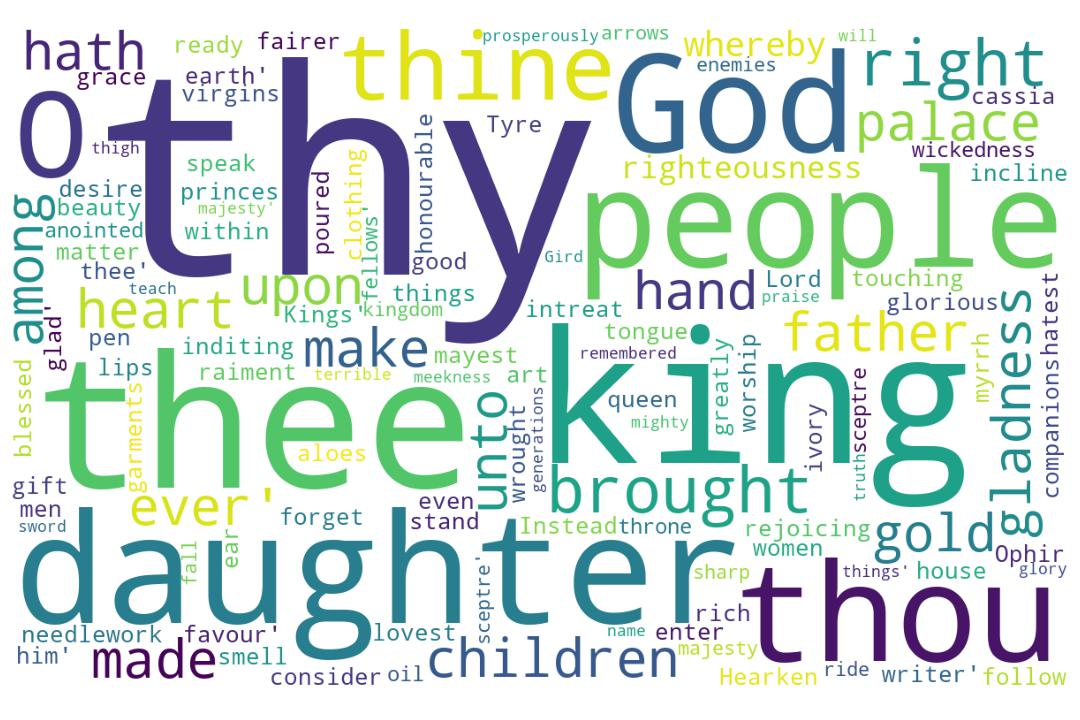
\includegraphics[width=\linewidth]{19OT-Psalms/Psalm45-WordCloud.jpg}
  \caption{Psalm 45 Word Cloud}
  \label{fig:Psalm 45 word Cloud}
\end{figure}

\marginpar{\scriptsize \centering \fcolorbox{bone}{lime}{\textbf{THE WEDDING SCENE}}\\ (Psalm 45:1-17) \begin{compactenum}[I.][8]
    \item A \textbf{Great Husband} \index[scripture]{Psalms!Psa 045:02}(Psa 45:2)
    \item \textbf{Glory \& } \index[scripture]{Psalms!Psa 045:08}(Psa 45:8)
    \item \textbf{Gladness \& Happiness} \index[scripture]{Psalms!Psa 045:07}(Psa 45:7)
    \item The \textbf{Groom is Here} \index[scripture]{Psalms!Psa 045:08}(Psa 45:8)
    \item The \textbf{Guests on High} (one theologian argues -- and I agree -- that the wedding guests will include believers from all ages, such as those before the Law, Gentile believers during the Law, etc -- all there to witness the Lord and His bride)\index[scripture]{Psalms!Psa 045:08}(Psa 45:8)
    \item \textbf{Gifts handed over} \index[scripture]{Psalms!Psa 045:12}(Psa 45:12)
    \item The \textbf{Gown and Handmaidens} \index[scripture]{Psalms!Psa 045:14}(Psa 45:14)
\end{compactenum}}

\footnote{\textcolor[cmyk]{0.99998,1,0,0}{\hyperlink{TOC}{Return to end of Table of Contents.}}}\footnote{\href{https://www.audioverse.org/english/audiobibles/books/ENGKJV/O/Ps/1}{\textcolor[cmyk]{0.99998,1,0,0}{Psalms Audio}}}\textcolor[cmyk]{0.99998,1,0,0}{To the chief Musician upon Shoshannim, for the sons of Korah, Mashil, A Song of loves}\footnote{\textbf{Revelation 19:7-10} - Let us be glad and rejoice, and give honour to him: for the marriage of the Lamb is come, and his wife hath made herself ready. [8] And to her was granted that she should be arrayed in fine linen, clean and white: for the fine linen is the righteousness of saints. [9] And he saith unto me, Write, Blessed are they which are called unto the marriage supper of the Lamb. And he saith unto me, These are the true sayings of God. [10] And I fell at his feet to worship him. And he said unto me, See thou do it not: I am thy fellowservant, and of thy brethren that have the testimony of Jesus: worship God: for the testimony of Jesus is the spirit of prophecy.}\\
\\
\textcolor[cmyk]{0.99998,1,0,0}{My heart is inditing a good matter: I speak of the things which I have made touching the king: my tongue \emph{is} the pen of a ready writer.}
[2] \textcolor[cmyk]{0.99998,1,0,0}{Thou art fairer than the children of men: grace is poured into thy lips: therefore God hath blessed thee for ever.}
[3] \textcolor[cmyk]{0.99998,1,0,0}{Gird thy sword upon \emph{thy} thigh, O \emph{most} mighty, with thy glory and thy majesty.}\footnote{\textbf{Genesis 3:24} - So he drove out the man; and he placed at the east of the garden of Eden Cherubims, and a flaming sword which turned every way, to keep the way of the tree of life.}\footnote{\textbf{Joshua 5:13-15} - And it came to pass, when Joshua was by Jericho, that he lifted up his eyes and looked, and, behold, there stood a man over against him with his sword drawn in his hand: and Joshua went unto him, and said unto him, Art thou for us, or for our adversaries? [14] And he said, Nay; but as captain of the host of the LORD am I now come. And Joshua fell on his face to the earth, and did worship, and said unto him, What saith my lord unto his servant? [15] And the captain of the LORD’S host said unto Joshua, Loose thy shoe from off thy foot; for the place whereon thou standest is holy. And Joshua did so.}\footnote{\textbf{Hebrews 4:12} - For the word of God is quick, and powerful, and sharper than any twoedged sword, piercing even to the dividing asunder of soul and spirit, and of the joints and marrow, and is a discerner of the thoughts and intents of the heart.}\footnote{\textbf{Revelation 19:15} - And out of his mouth goeth a sharp sword, that with it he should smite the nations: and he shall rule them with a rod of iron: and he treadeth the winepress of the fierceness and wrath of Almighty God.}\footnote{\textbf{Revelation 19:21} - And the remnant were slain with the sword of him that sat upon the horse, which sword proceeded out of his mouth: and all the fowls were filled with their flesh.} 
[4] \textcolor[cmyk]{0.99998,1,0,0}{And in thy majesty ride prosperously because of truth and meekness \emph{and} \fcolorbox{bone}{MYGOLD}{righteousness}; and thy right hand shall teach thee terrible things.}
[5] \textcolor[cmyk]{0.99998,1,0,0}{Thine arrows \emph{are} sharp in the heart of the king's enemies; \emph{whereby} the people fall under thee.}
[6] \textcolor[cmyk]{0.99998,1,0,0}{Thy throne, O God, \emph{is} for ever and ever: the sceptre of thy kingdom \emph{is} a right sceptre.}
[7] \textcolor[cmyk]{0.99998,1,0,0}{Thou lovest \fcolorbox{bone}{MYGOLD}{righteousness}, and hatest wickedness: therefore God, thy God, hath anointed thee with the oil of gladness above thy fellows.}
[8] \textcolor[cmyk]{0.99998,1,0,0}{All thy garments \emph{smell} of myrrh, and aloes, \emph{and} cassia, out of the ivory palaces, whereby they have made thee glad.}
[9] \textcolor[cmyk]{0.99998,1,0,0}{Kings' daughters \emph{were} among thy honourable women: upon thy right hand did stand the queen in gold of Ophir.}
[10] \textcolor[cmyk]{0.99998,1,0,0}{Hearken, O daughter, and consider, and incline thine ear; forget also thine own people, and thy father's house;}
[11] \textcolor[cmyk]{0.99998,1,0,0}{So shall the king greatly desire thy beauty: for he \emph{is} thy Lord; and worship thou him.}
[12] \textcolor[cmyk]{0.99998,1,0,0}{And the daughter of Tyre \emph{shall} \emph{be} \emph{there} with a gift; \emph{even} the rich among the people shall intreat thy favour.}
[13] \textcolor[cmyk]{0.99998,1,0,0}{The king's daughter \emph{is} all glorious within: her clothing \emph{is} of wrought gold.}
[14] \textcolor[cmyk]{0.99998,1,0,0}{She shall be brought unto the king in raiment of needlework: the virgins her companions that follow her shall be brought unto thee.}
[15] \textcolor[cmyk]{0.99998,1,0,0}{With gladness and rejoicing shall they be brought: they shall enter into the king's palace.}
[16] \textcolor[cmyk]{0.99998,1,0,0}{Instead of thy fathers shall be thy children, whom thou mayest make princes in all the earth.}
[17] \textcolor[cmyk]{0.99998,1,0,0}{I will make thy name to be remembered in all generations: therefore shall the people praise thee for ever and ever.}


\index[NWIV]{28!Psalms!Psa 45:1}\index[AWIP]{My!Psalms!Psa 45:1}\index[AWIP]{heart!Psalms!Psa 45:1}\index[AWIP]{is!Psalms!Psa 45:1}\index[AWIP]{inditing!Psalms!Psa 45:1}\index[AWIP]{a!Psalms!Psa 45:1}\index[AWIP]{a!Psalms!Psa 45:1 (2)}\index[AWIP]{good!Psalms!Psa 45:1}\index[AWIP]{matter!Psalms!Psa 45:1}\index[AWIP]{I!Psalms!Psa 45:1}\index[AWIP]{I!Psalms!Psa 45:1 (2)}\index[AWIP]{speak!Psalms!Psa 45:1}\index[AWIP]{of!Psalms!Psa 45:1}\index[AWIP]{of!Psalms!Psa 45:1 (2)}\index[AWIP]{the!Psalms!Psa 45:1}\index[AWIP]{the!Psalms!Psa 45:1 (2)}\index[AWIP]{the!Psalms!Psa 45:1 (3)}\index[AWIP]{things!Psalms!Psa 45:1}\index[AWIP]{which!Psalms!Psa 45:1}\index[AWIP]{have!Psalms!Psa 45:1}\index[AWIP]{made!Psalms!Psa 45:1}\index[AWIP]{touching!Psalms!Psa 45:1}\index[AWIP]{king!Psalms!Psa 45:1}\index[AWIP]{my!Psalms!Psa 45:1}\index[AWIP]{tongue!Psalms!Psa 45:1}\index[AWIP]{\emph{is}!Psalms!Psa 45:1}\index[AWIP]{pen!Psalms!Psa 45:1}\index[AWIP]{ready!Psalms!Psa 45:1}\index[AWIP]{writer!Psalms!Psa 45:1}\index[AWIP]{\emph{is}!Psalms!Psa 45:1}

\index[NWIV]{21!Psalms!Psa 45:2}\index[AWIP]{Thou!Psalms!Psa 45:2}\index[AWIP]{art!Psalms!Psa 45:2}\index[AWIP]{fairer!Psalms!Psa 45:2}\index[AWIP]{than!Psalms!Psa 45:2}\index[AWIP]{the!Psalms!Psa 45:2}\index[AWIP]{children!Psalms!Psa 45:2}\index[AWIP]{of!Psalms!Psa 45:2}\index[AWIP]{men!Psalms!Psa 45:2}\index[AWIP]{grace!Psalms!Psa 45:2}\index[AWIP]{is!Psalms!Psa 45:2}\index[AWIP]{poured!Psalms!Psa 45:2}\index[AWIP]{into!Psalms!Psa 45:2}\index[AWIP]{thy!Psalms!Psa 45:2}\index[AWIP]{lips!Psalms!Psa 45:2}\index[AWIP]{therefore!Psalms!Psa 45:2}\index[AWIP]{God!Psalms!Psa 45:2}\index[AWIP]{hath!Psalms!Psa 45:2}\index[AWIP]{blessed!Psalms!Psa 45:2}\index[AWIP]{thee!Psalms!Psa 45:2}\index[AWIP]{for!Psalms!Psa 45:2}\index[AWIP]{ever!Psalms!Psa 45:2}

\index[NWIV]{15!Psalms!Psa 45:3}\index[AWIP]{Gird!Psalms!Psa 45:3}\index[AWIP]{thy!Psalms!Psa 45:3}\index[AWIP]{thy!Psalms!Psa 45:3 (2)}\index[AWIP]{thy!Psalms!Psa 45:3 (3)}\index[AWIP]{sword!Psalms!Psa 45:3}\index[AWIP]{upon!Psalms!Psa 45:3}\index[AWIP]{\emph{thy}!Psalms!Psa 45:3}\index[AWIP]{thigh!Psalms!Psa 45:3}\index[AWIP]{O!Psalms!Psa 45:3}\index[AWIP]{\emph{most}!Psalms!Psa 45:3}\index[AWIP]{mighty!Psalms!Psa 45:3}\index[AWIP]{with!Psalms!Psa 45:3}\index[AWIP]{glory!Psalms!Psa 45:3}\index[AWIP]{and!Psalms!Psa 45:3}\index[AWIP]{majesty!Psalms!Psa 45:3}\index[AWIP]{\emph{thy}!Psalms!Psa 45:3}\index[AWIP]{\emph{most}!Psalms!Psa 45:3}

\index[NWIV]{22!Psalms!Psa 45:4}\index[AWIP]{And!Psalms!Psa 45:4}\index[AWIP]{in!Psalms!Psa 45:4}\index[AWIP]{thy!Psalms!Psa 45:4}\index[AWIP]{thy!Psalms!Psa 45:4 (2)}\index[AWIP]{majesty!Psalms!Psa 45:4}\index[AWIP]{ride!Psalms!Psa 45:4}\index[AWIP]{prosperously!Psalms!Psa 45:4}\index[AWIP]{because!Psalms!Psa 45:4}\index[AWIP]{of!Psalms!Psa 45:4}\index[AWIP]{truth!Psalms!Psa 45:4}\index[AWIP]{and!Psalms!Psa 45:4}\index[AWIP]{and!Psalms!Psa 45:4 (2)}\index[AWIP]{meekness!Psalms!Psa 45:4}\index[AWIP]{\emph{and}!Psalms!Psa 45:4}\index[AWIP]{righteousness!Psalms!Psa 45:4}\index[AWIP]{right!Psalms!Psa 45:4}\index[AWIP]{hand!Psalms!Psa 45:4}\index[AWIP]{shall!Psalms!Psa 45:4}\index[AWIP]{teach!Psalms!Psa 45:4}\index[AWIP]{thee!Psalms!Psa 45:4}\index[AWIP]{terrible!Psalms!Psa 45:4}\index[AWIP]{things!Psalms!Psa 45:4}\index[AWIP]{\emph{and}!Psalms!Psa 45:4}

\index[NWIV]{17!Psalms!Psa 45:5}\index[AWIP]{Thine!Psalms!Psa 45:5}\index[AWIP]{arrows!Psalms!Psa 45:5}\index[AWIP]{\emph{are}!Psalms!Psa 45:5}\index[AWIP]{sharp!Psalms!Psa 45:5}\index[AWIP]{in!Psalms!Psa 45:5}\index[AWIP]{the!Psalms!Psa 45:5}\index[AWIP]{the!Psalms!Psa 45:5 (2)}\index[AWIP]{the!Psalms!Psa 45:5 (3)}\index[AWIP]{heart!Psalms!Psa 45:5}\index[AWIP]{of!Psalms!Psa 45:5}\index[AWIP]{king's!Psalms!Psa 45:5}\index[AWIP]{enemies!Psalms!Psa 45:5}\index[AWIP]{\emph{whereby}!Psalms!Psa 45:5}\index[AWIP]{people!Psalms!Psa 45:5}\index[AWIP]{fall!Psalms!Psa 45:5}\index[AWIP]{under!Psalms!Psa 45:5}\index[AWIP]{thee!Psalms!Psa 45:5}\index[AWIP]{\emph{are}!Psalms!Psa 45:5}\index[AWIP]{\emph{whereby}!Psalms!Psa 45:5}

\index[NWIV]{18!Psalms!Psa 45:6}\index[AWIP]{Thy!Psalms!Psa 45:6}\index[AWIP]{throne!Psalms!Psa 45:6}\index[AWIP]{O!Psalms!Psa 45:6}\index[AWIP]{God!Psalms!Psa 45:6}\index[AWIP]{\emph{is}!Psalms!Psa 45:6}\index[AWIP]{\emph{is}!Psalms!Psa 45:6 (2)}\index[AWIP]{for!Psalms!Psa 45:6}\index[AWIP]{ever!Psalms!Psa 45:6}\index[AWIP]{ever!Psalms!Psa 45:6 (2)}\index[AWIP]{and!Psalms!Psa 45:6}\index[AWIP]{the!Psalms!Psa 45:6}\index[AWIP]{sceptre!Psalms!Psa 45:6}\index[AWIP]{sceptre!Psalms!Psa 45:6 (2)}\index[AWIP]{of!Psalms!Psa 45:6}\index[AWIP]{thy!Psalms!Psa 45:6}\index[AWIP]{kingdom!Psalms!Psa 45:6}\index[AWIP]{a!Psalms!Psa 45:6}\index[AWIP]{right!Psalms!Psa 45:6}\index[AWIP]{\emph{is}!Psalms!Psa 45:6}\index[AWIP]{\emph{is}!Psalms!Psa 45:6 (2)}

\index[NWIV]{21!Psalms!Psa 45:7}\index[AWIP]{Thou!Psalms!Psa 45:7}\index[AWIP]{lovest!Psalms!Psa 45:7}\index[AWIP]{righteousness!Psalms!Psa 45:7}\index[AWIP]{and!Psalms!Psa 45:7}\index[AWIP]{hatest!Psalms!Psa 45:7}\index[AWIP]{wickedness!Psalms!Psa 45:7}\index[AWIP]{therefore!Psalms!Psa 45:7}\index[AWIP]{God!Psalms!Psa 45:7}\index[AWIP]{God!Psalms!Psa 45:7 (2)}\index[AWIP]{thy!Psalms!Psa 45:7}\index[AWIP]{thy!Psalms!Psa 45:7 (2)}\index[AWIP]{hath!Psalms!Psa 45:7}\index[AWIP]{anointed!Psalms!Psa 45:7}\index[AWIP]{thee!Psalms!Psa 45:7}\index[AWIP]{with!Psalms!Psa 45:7}\index[AWIP]{the!Psalms!Psa 45:7}\index[AWIP]{oil!Psalms!Psa 45:7}\index[AWIP]{of!Psalms!Psa 45:7}\index[AWIP]{gladness!Psalms!Psa 45:7}\index[AWIP]{above!Psalms!Psa 45:7}\index[AWIP]{fellows!Psalms!Psa 45:7}

\index[NWIV]{21!Psalms!Psa 45:8}\index[AWIP]{All!Psalms!Psa 45:8}\index[AWIP]{thy!Psalms!Psa 45:8}\index[AWIP]{garments!Psalms!Psa 45:8}\index[AWIP]{\emph{smell}!Psalms!Psa 45:8}\index[AWIP]{of!Psalms!Psa 45:8}\index[AWIP]{of!Psalms!Psa 45:8 (2)}\index[AWIP]{myrrh!Psalms!Psa 45:8}\index[AWIP]{and!Psalms!Psa 45:8}\index[AWIP]{aloes!Psalms!Psa 45:8}\index[AWIP]{\emph{and}!Psalms!Psa 45:8}\index[AWIP]{cassia!Psalms!Psa 45:8}\index[AWIP]{out!Psalms!Psa 45:8}\index[AWIP]{the!Psalms!Psa 45:8}\index[AWIP]{ivory!Psalms!Psa 45:8}\index[AWIP]{palaces!Psalms!Psa 45:8}\index[AWIP]{whereby!Psalms!Psa 45:8}\index[AWIP]{they!Psalms!Psa 45:8}\index[AWIP]{have!Psalms!Psa 45:8}\index[AWIP]{made!Psalms!Psa 45:8}\index[AWIP]{thee!Psalms!Psa 45:8}\index[AWIP]{glad!Psalms!Psa 45:8}\index[AWIP]{\emph{smell}!Psalms!Psa 45:8}\index[AWIP]{\emph{and}!Psalms!Psa 45:8}

\index[NWIV]{19!Psalms!Psa 45:9}\index[AWIP]{Kings'!Psalms!Psa 45:9}\index[AWIP]{daughters!Psalms!Psa 45:9}\index[AWIP]{\emph{were}!Psalms!Psa 45:9}\index[AWIP]{among!Psalms!Psa 45:9}\index[AWIP]{thy!Psalms!Psa 45:9}\index[AWIP]{thy!Psalms!Psa 45:9 (2)}\index[AWIP]{honourable!Psalms!Psa 45:9}\index[AWIP]{women!Psalms!Psa 45:9}\index[AWIP]{upon!Psalms!Psa 45:9}\index[AWIP]{right!Psalms!Psa 45:9}\index[AWIP]{hand!Psalms!Psa 45:9}\index[AWIP]{did!Psalms!Psa 45:9}\index[AWIP]{stand!Psalms!Psa 45:9}\index[AWIP]{the!Psalms!Psa 45:9}\index[AWIP]{queen!Psalms!Psa 45:9}\index[AWIP]{in!Psalms!Psa 45:9}\index[AWIP]{gold!Psalms!Psa 45:9}\index[AWIP]{of!Psalms!Psa 45:9}\index[AWIP]{Ophir!Psalms!Psa 45:9}\index[AWIP]{\emph{were}!Psalms!Psa 45:9}

\index[NWIV]{18!Psalms!Psa 45:10}\index[AWIP]{Hearken!Psalms!Psa 45:10}\index[AWIP]{O!Psalms!Psa 45:10}\index[AWIP]{daughter!Psalms!Psa 45:10}\index[AWIP]{and!Psalms!Psa 45:10}\index[AWIP]{and!Psalms!Psa 45:10 (2)}\index[AWIP]{and!Psalms!Psa 45:10 (3)}\index[AWIP]{consider!Psalms!Psa 45:10}\index[AWIP]{incline!Psalms!Psa 45:10}\index[AWIP]{thine!Psalms!Psa 45:10}\index[AWIP]{thine!Psalms!Psa 45:10 (2)}\index[AWIP]{ear!Psalms!Psa 45:10}\index[AWIP]{forget!Psalms!Psa 45:10}\index[AWIP]{also!Psalms!Psa 45:10}\index[AWIP]{own!Psalms!Psa 45:10}\index[AWIP]{people!Psalms!Psa 45:10}\index[AWIP]{thy!Psalms!Psa 45:10}\index[AWIP]{father's!Psalms!Psa 45:10}\index[AWIP]{house!Psalms!Psa 45:10}

\index[NWIV]{17!Psalms!Psa 45:11}\index[AWIP]{So!Psalms!Psa 45:11}\index[AWIP]{shall!Psalms!Psa 45:11}\index[AWIP]{the!Psalms!Psa 45:11}\index[AWIP]{king!Psalms!Psa 45:11}\index[AWIP]{greatly!Psalms!Psa 45:11}\index[AWIP]{desire!Psalms!Psa 45:11}\index[AWIP]{thy!Psalms!Psa 45:11}\index[AWIP]{thy!Psalms!Psa 45:11 (2)}\index[AWIP]{beauty!Psalms!Psa 45:11}\index[AWIP]{for!Psalms!Psa 45:11}\index[AWIP]{he!Psalms!Psa 45:11}\index[AWIP]{\emph{is}!Psalms!Psa 45:11}\index[AWIP]{Lord!Psalms!Psa 45:11}\index[AWIP]{and!Psalms!Psa 45:11}\index[AWIP]{worship!Psalms!Psa 45:11}\index[AWIP]{thou!Psalms!Psa 45:11}\index[AWIP]{him!Psalms!Psa 45:11}\index[AWIP]{\emph{is}!Psalms!Psa 45:11}

\index[NWIV]{21!Psalms!Psa 45:12}\index[AWIP]{And!Psalms!Psa 45:12}\index[AWIP]{the!Psalms!Psa 45:12}\index[AWIP]{the!Psalms!Psa 45:12 (2)}\index[AWIP]{the!Psalms!Psa 45:12 (3)}\index[AWIP]{daughter!Psalms!Psa 45:12}\index[AWIP]{of!Psalms!Psa 45:12}\index[AWIP]{Tyre!Psalms!Psa 45:12}\index[AWIP]{\emph{shall}!Psalms!Psa 45:12}\index[AWIP]{\emph{be}!Psalms!Psa 45:12}\index[AWIP]{\emph{there}!Psalms!Psa 45:12}\index[AWIP]{with!Psalms!Psa 45:12}\index[AWIP]{a!Psalms!Psa 45:12}\index[AWIP]{gift!Psalms!Psa 45:12}\index[AWIP]{\emph{even}!Psalms!Psa 45:12}\index[AWIP]{rich!Psalms!Psa 45:12}\index[AWIP]{among!Psalms!Psa 45:12}\index[AWIP]{people!Psalms!Psa 45:12}\index[AWIP]{shall!Psalms!Psa 45:12}\index[AWIP]{intreat!Psalms!Psa 45:12}\index[AWIP]{thy!Psalms!Psa 45:12}\index[AWIP]{favour!Psalms!Psa 45:12}\index[AWIP]{\emph{shall}!Psalms!Psa 45:12}\index[AWIP]{\emph{be}!Psalms!Psa 45:12}\index[AWIP]{\emph{there}!Psalms!Psa 45:12}\index[AWIP]{\emph{even}!Psalms!Psa 45:12}

\index[NWIV]{13!Psalms!Psa 45:13}\index[AWIP]{The!Psalms!Psa 45:13}\index[AWIP]{king's!Psalms!Psa 45:13}\index[AWIP]{daughter!Psalms!Psa 45:13}\index[AWIP]{\emph{is}!Psalms!Psa 45:13}\index[AWIP]{\emph{is}!Psalms!Psa 45:13 (2)}\index[AWIP]{all!Psalms!Psa 45:13}\index[AWIP]{glorious!Psalms!Psa 45:13}\index[AWIP]{within!Psalms!Psa 45:13}\index[AWIP]{her!Psalms!Psa 45:13}\index[AWIP]{clothing!Psalms!Psa 45:13}\index[AWIP]{of!Psalms!Psa 45:13}\index[AWIP]{wrought!Psalms!Psa 45:13}\index[AWIP]{gold!Psalms!Psa 45:13}\index[AWIP]{\emph{is}!Psalms!Psa 45:13}\index[AWIP]{\emph{is}!Psalms!Psa 45:13 (2)}

\index[NWIV]{23!Psalms!Psa 45:14}\index[AWIP]{She!Psalms!Psa 45:14}\index[AWIP]{shall!Psalms!Psa 45:14}\index[AWIP]{shall!Psalms!Psa 45:14 (2)}\index[AWIP]{be!Psalms!Psa 45:14}\index[AWIP]{be!Psalms!Psa 45:14 (2)}\index[AWIP]{brought!Psalms!Psa 45:14}\index[AWIP]{brought!Psalms!Psa 45:14 (2)}\index[AWIP]{unto!Psalms!Psa 45:14}\index[AWIP]{unto!Psalms!Psa 45:14 (2)}\index[AWIP]{the!Psalms!Psa 45:14}\index[AWIP]{the!Psalms!Psa 45:14 (2)}\index[AWIP]{king!Psalms!Psa 45:14}\index[AWIP]{in!Psalms!Psa 45:14}\index[AWIP]{raiment!Psalms!Psa 45:14}\index[AWIP]{of!Psalms!Psa 45:14}\index[AWIP]{needlework!Psalms!Psa 45:14}\index[AWIP]{virgins!Psalms!Psa 45:14}\index[AWIP]{her!Psalms!Psa 45:14}\index[AWIP]{her!Psalms!Psa 45:14 (2)}\index[AWIP]{companions!Psalms!Psa 45:14}\index[AWIP]{that!Psalms!Psa 45:14}\index[AWIP]{follow!Psalms!Psa 45:14}\index[AWIP]{thee!Psalms!Psa 45:14}

\index[NWIV]{15!Psalms!Psa 45:15}\index[AWIP]{With!Psalms!Psa 45:15}\index[AWIP]{gladness!Psalms!Psa 45:15}\index[AWIP]{and!Psalms!Psa 45:15}\index[AWIP]{rejoicing!Psalms!Psa 45:15}\index[AWIP]{shall!Psalms!Psa 45:15}\index[AWIP]{shall!Psalms!Psa 45:15 (2)}\index[AWIP]{they!Psalms!Psa 45:15}\index[AWIP]{they!Psalms!Psa 45:15 (2)}\index[AWIP]{be!Psalms!Psa 45:15}\index[AWIP]{brought!Psalms!Psa 45:15}\index[AWIP]{enter!Psalms!Psa 45:15}\index[AWIP]{into!Psalms!Psa 45:15}\index[AWIP]{the!Psalms!Psa 45:15}\index[AWIP]{king's!Psalms!Psa 45:15}\index[AWIP]{palace!Psalms!Psa 45:15}

\index[NWIV]{17!Psalms!Psa 45:16}\index[AWIP]{Instead!Psalms!Psa 45:16}\index[AWIP]{of!Psalms!Psa 45:16}\index[AWIP]{thy!Psalms!Psa 45:16}\index[AWIP]{thy!Psalms!Psa 45:16 (2)}\index[AWIP]{fathers!Psalms!Psa 45:16}\index[AWIP]{shall!Psalms!Psa 45:16}\index[AWIP]{be!Psalms!Psa 45:16}\index[AWIP]{children!Psalms!Psa 45:16}\index[AWIP]{whom!Psalms!Psa 45:16}\index[AWIP]{thou!Psalms!Psa 45:16}\index[AWIP]{mayest!Psalms!Psa 45:16}\index[AWIP]{make!Psalms!Psa 45:16}\index[AWIP]{princes!Psalms!Psa 45:16}\index[AWIP]{in!Psalms!Psa 45:16}\index[AWIP]{all!Psalms!Psa 45:16}\index[AWIP]{the!Psalms!Psa 45:16}\index[AWIP]{earth!Psalms!Psa 45:16}

\index[NWIV]{21!Psalms!Psa 45:17}\index[AWIP]{I!Psalms!Psa 45:17}\index[AWIP]{will!Psalms!Psa 45:17}\index[AWIP]{make!Psalms!Psa 45:17}\index[AWIP]{thy!Psalms!Psa 45:17}\index[AWIP]{name!Psalms!Psa 45:17}\index[AWIP]{to!Psalms!Psa 45:17}\index[AWIP]{be!Psalms!Psa 45:17}\index[AWIP]{remembered!Psalms!Psa 45:17}\index[AWIP]{in!Psalms!Psa 45:17}\index[AWIP]{all!Psalms!Psa 45:17}\index[AWIP]{generations!Psalms!Psa 45:17}\index[AWIP]{therefore!Psalms!Psa 45:17}\index[AWIP]{shall!Psalms!Psa 45:17}\index[AWIP]{the!Psalms!Psa 45:17}\index[AWIP]{people!Psalms!Psa 45:17}\index[AWIP]{praise!Psalms!Psa 45:17}\index[AWIP]{thee!Psalms!Psa 45:17}\index[AWIP]{for!Psalms!Psa 45:17}\index[AWIP]{ever!Psalms!Psa 45:17}\index[AWIP]{ever!Psalms!Psa 45:17 (2)}\index[AWIP]{and!Psalms!Psa 45:17}


\section{Psalm 45 Outlines}

\subsection{My Outlines}

\subsubsection{The Wedding Scene}
\textbf{Introduction:} All of what we expect at a wedding, but on a grand and glorious scale! 
\index[speaker]{Keith Anthony!Psalm 045 (The Wedding Scene)}
\index[series]{Psalms (Keith Anthony)!Psalm 045 (The Wedding Scene)}
\index[date]{2017/02/14!Psalm 045 (The Wedding Scene) (Keith Anthony)}

\begin{compactenum}[I.][19]
    \item A \textbf{Great Husband} \index[scripture]{Psalms!Psa 045:02}(Psa 45:2)
    \item \textbf{Glory \& } \index[scripture]{Psalms!Psa 045:08}(Psa 45:8)
    \item \textbf{Gladness \& Happiness} \index[scripture]{Psalms!Psa 045:07}(Psa 45:7)
    \item The \textbf{Groom is Here} \index[scripture]{Psalms!Psa 045:08}(Psa 45:8)
    \item The \textbf{Guests on High} (one theologian argues -- and I agree -- that the wedding guests will include believers from all ages, such as those before the Law, Gentile believers during the Law, etc -- all there to witness the Lord and His bride)\index[scripture]{Psalms!Psa 045:08}(Psa 45:8)
    \item \textbf{Gifts handed over} \index[scripture]{Psalms!Psa 045:12}(Psa 45:12)
    \item The \textbf{Gown and Handmaidens} \index[scripture]{Psalms!Psa 045:14}(Psa 45:14)
\end{compactenum}

\subsection{Outlines from Others}




\section{Psalm 45 Comments}

\subsection{Numeric Nuggets}
There are 13 words in verse 13. Verses 3 and 15 contain 13 unique words. The 13-letter word ``righteousness'' is found in the chapter.

\subsection{Psalm 45 Introduction}
The passage is  understood by identifying the actors in the it and getting the events in chronological order. As pointed out by Ruckman, the events are presented out of chronological order, as in done in Psalm 44:8-9 and as in done in Psalm 43.\cite{Ruckman1992Psalms} Psalm 45 describes, first, events at the Second Advent (see references to the sword) and then back to something that happens before that, the marriage of the Lamb. Verses 8 through 16 talk about the groups of people who will be attending the wedding!

\subsection{Psalm 45:5}
The phrase ``thine arrows'' is clearly a Second Advent reference, as indicated by the seven times it is used: (1) Psalms 21:12 , (2) Psalms 38:2, (3) Psalms 45:5, (4) Psalms 77:17, (5) Psalms 144:6, (6) Ezekiel 39:3, and (7) Habakkuk 3:11.

\subsubsection{The word ``king's"}

Consider the things of kings as told to us in 284 references of the word ``king's'':
\begin{compactenum}
    \item the king's burnt sacrifice (2 Kings 16:15)
    \item the King's commandment (2 Kings 18:36)
    \item the king's \emph{cost} (2 Samuel 19:42)
    \item the king's crown (2 Samuel 12:30)
    \item the king's dale (Genesis 14:17; 2 Samuel 18:18)
    \item the king's daughter (2 Kings 9:34)
    \item the king's daughters (2 Samuel 13:18)
    \item the king's enemies (1 Samuel 18:25)
    \item the king's entry (2 Kings 16:18)
    \item the king's face (2 Samuel 14:24, 28, 32)
    \item the king's friend (1 Kings 4:5)
    \item the king's garden (2 Kings 25:4)
    \item the king's gate (1 Chronicles 9:18)
    \item the king's hand (1 Samuel 23:20; 1 Kings 13:6, 1 Kings 22:12
    \item the king's hands (2 Kings 13:16)
    \item the king's heart (2 Samuel 14:1)
    \item the king's \emph{high} way (Numbers 20:17, 21:22)
    \item the king's house (2 Samuel 11:2, 8, 9; 15:35; 1 Kings 9:10, 10:12, 14:26, 27, 15:18, 16:18 (2x); 2 Kings 7:11, 11:5, 16, 20, 12:13, 14:14, 15:25, 16:8, 18:15; 24:13, 25:9)
    \item the king's household (2 Samuel 16:2; 2 Kings 7:9)
    \item the king's merchants (1 Kings 10:28)
    \item the king's mother (1 Kings 2:19; 2 Kings 24:15)
    \item the king's mule (1 Kings 1:44)
    \item the king's order (1 Chronicles 25:6)
    \item the king's presence (1 Kings 1:28; 2 Kings 25:19)
    \item the king's prisoners (Genesis 39:20)
    \item the king's scribe (2 Kings 12:10)
    \item the king's seed (a Kings 11:14)
    \item the king's seer (1 Chronicles 25:5)
    \item the king's servant (2 Samuel 18:29; 2 Kings 22:12)
    \item the king's servants (2 Samuel 11:24; 15:15; 1 Kings 1:9, 47)
    \item the king's son (2 Samuel 13:4; 18:12, 20; 2 Kings 11:4, 11:12, 15:5)
    \item the king's son in law (1 Samuel 18:22, 26, 27; 22:14; 1 Kings 22:26)
    \item the king's sons (2 Samuel 9:11; 13:23, 27, 29, 30, 32, 33, 35, 36; 1 Kings 1:9, 25; 2 Kings 10:6, 7, 8, 11:2)
    \item the king's spear (1 Samuel 26:22)
    \item the king's table (1 Samuel 20:29; 2 Samuel 9:13)
    \item the king's weight (2 Samuel 14:26)
    \item the king's wives (2 Kings 24:15)
    \item the king's word (2 Samuel 24:4, 1 Chronicles 21:4, 6)
    \item the king's wrath (2 Samuel 11:20)
\end{compactenum}
\textbf{}


\subsection{Psalm 45:6}
First occurrence of ``sceptre'' is Jacob's prophecy for the tribe of Judah in Genesis 49:10.\footnote{\textbf{Genesis 49:10} - The sceptre shall not depart from Judah, nor a lawgiver from between his feet, until Shiloh come; and unto him shall the gathering of the people be.} The last occurrence is in Hebrews 1:8.\footnote{\textbf{Hebrews 1:8} - But unto the Son he saith, Thy throne, O God, is for ever and ever: a sceptre of righteousness is the sceptre of thy kingdom.} The single occurrence of the capitalized word ``Sceptre'' is in Numbers 24:17 spoken by Balaam.\footnote{\textbf{Numbers 24:17} - I shall see him, but not now: I shall behold him, but not nigh: there shall come a Star out of Jacob, and a Sceptre shall rise out of Israel, and shall smite the corners of Moab, and destroy all the children of Sheth.}

\subsection{Psalm45 Repeated Phrases}


%%%%%%%%%%
%%%%%%%%%%
\normalsize
 
\begin{center}
\begin{longtable}{|c|c|}
\caption[Psalm45 Repeated Phrases]{Psalm45 Repeated Phrases}\label{table:Repeated Phrases Psalm45} \\
\hline \multicolumn{1}{|c|}{\textbf{Phrase}} & \multicolumn{1}{c|}{\textbf{Frequency}} \\ \hline 
\endfirsthead
 
\multicolumn{2}{c}
{{\bfseries \tablename\ \thetable{} -- continued from previous page}} \\  
\hline \multicolumn{1}{|c|}{\textbf{Phrase}} & \multicolumn{1}{c|}{\textbf{Frequency}} \\ \hline 
\endhead
 
\hline \multicolumn{2}{c}{{ }} \\ \hline
\endfoot 
of the & 3\\ \hline 
the king & 3\\ \hline 
for ever & 3\\ \hline 
and thy & 3\\ \hline 
the people & 3\\ \hline 
shall be & 3\\ \hline 
be brought & 3\\ \hline 
\end{longtable}
\end{center}



%%%%%%%%%%
%%%%%%%%%%



\section{Psalm 45 Word Statistics}


%%%%%%%%%%
%%%%%%%%%%
\normalsize
 
\begin{center}
\begin{longtable}{l|c|c|c|c}
\caption[Psalm 45 Statistics]{Psalm 45 Statistics}\label{table:Statistics for Psalm 45} \\
\hline \multicolumn{1}{|c|}{\textbf{Verse(s)}} & \multicolumn{1}{|c|}{\textbf{Count}} & \multicolumn{1}{|c|}{\textbf{Unique}} & \multicolumn{1}{|c|}{\textbf{Italics}} & \multicolumn{1}{|c|}{\textbf{Uniq Italic}}  \\ \hline 
\endfirsthead
 
\multicolumn{5}{c}
{{\bfseries \tablename\ \thetable{} -- continued from previous page}} \\  
\hline \multicolumn{1}{|c|}{\textbf{Verse(s)}} & \multicolumn{1}{|c|}{\textbf{Count}} & \multicolumn{1}{|c|}{\textbf{Unique}} & \multicolumn{1}{|c|}{\textbf{Italics}} & \multicolumn{1}{|c|}{\textbf{Uniq Italic}}  \\ \hline 
\endhead
 
\hline \multicolumn{5}{|r|}{{}} \\ \hline
\endfoot 
1 & 28 & 23 & 1 & 1\\ \hline
2 & 21 & 21 & 0 & 0\\ \hline
3 & 15 & 13 & 2 & 2\\ \hline
4 & 22 & 20 & 1 & 1\\ \hline
5 & 17 & 15 & 2 & 2\\ \hline
6 & 18 & 15 & 2 & 1\\ \hline
7 & 21 & 19 & 0 & 0\\ \hline
8 & 21 & 20 & 2 & 2\\ \hline
9 & 19 & 18 & 1 & 1\\ \hline
10 & 18 & 15 & 0 & 0\\ \hline
11 & 17 & 16 & 1 & 1\\ \hline
12 & 21 & 19 & 4 & 4\\ \hline
13 & 13 & 12 & 2 & 1\\ \hline
14 & 23 & 17 & 0 & 0\\ \hline
15 & 15 & 13 & 0 & 0\\ \hline
16 & 17 & 16 & 0 & 0\\ \hline
17 & 21 & 20 & 0 & 0\\ \hline
Total & 327 & 175 & 18 & 12
\end{longtable}
\end{center}



%%%%%%%%%%
%%%%%%%%%%


\subsection{Psalm 45 Words by Frequency}


%%%%%%%%%%
%%%%%%%%%%
\normalsize
 
\begin{center}
\begin{longtable}{l|r}
\caption[Psalm 45 Words by Frequency]{Psalm 45 Words by Frequency}\label{table:WordsbyFrequency for Psalm 45} \\
\hline \multicolumn{1}{|c|}{\textbf{Word}} & \multicolumn{1}{c|}{\textbf{Frequency}} \\ \hline 
\endfirsthead
 
\multicolumn{2}{c}
{{\bfseries \tablename\ \thetable{} -- continued from previous page}} \\  
\hline \multicolumn{1}{|c|}{\textbf{Word}} & \multicolumn{1}{c|}{\textbf{Frequency}} \\ \hline 
\endhead
 
\hline \multicolumn{2}{c}{{ }} \\ \hline
\endfoot 
the & 20\\ \hline 
thy & 19\\ \hline 
of & 14\\ \hline 
and & 12\\ \hline 
shall & 9\\ \hline 
thee & 7\\ \hline 
\emph{is} & 6\\ \hline 
in & 6\\ \hline 
ever & 5\\ \hline 
be & 5\\ \hline 
a & 4\\ \hline 
God & 4\\ \hline 
for & 4\\ \hline 
people & 4\\ \hline 
I & 3\\ \hline 
king & 3\\ \hline 
therefore & 3\\ \hline 
O & 3\\ \hline 
with & 3\\ \hline 
right & 3\\ \hline 
king's & 3\\ \hline 
they & 3\\ \hline 
daughter & 3\\ \hline 
all & 3\\ \hline 
her & 3\\ \hline 
brought & 3\\ \hline 
heart & 2\\ \hline 
is & 2\\ \hline 
things & 2\\ \hline 
have & 2\\ \hline 
made & 2\\ \hline 
Thou & 2\\ \hline 
children & 2\\ \hline 
into & 2\\ \hline 
hath & 2\\ \hline 
upon & 2\\ \hline 
majesty & 2\\ \hline 
And & 2\\ \hline 
\emph{and} & 2\\ \hline 
righteousness & 2\\ \hline 
hand & 2\\ \hline 
sceptre & 2\\ \hline 
gladness & 2\\ \hline 
among & 2\\ \hline 
gold & 2\\ \hline 
thine & 2\\ \hline 
thou & 2\\ \hline 
unto & 2\\ \hline 
make & 2\\ \hline 
My & 1\\ \hline 
inditing & 1\\ \hline 
good & 1\\ \hline 
matter & 1\\ \hline 
speak & 1\\ \hline 
which & 1\\ \hline 
touching & 1\\ \hline 
my & 1\\ \hline 
tongue & 1\\ \hline 
pen & 1\\ \hline 
ready & 1\\ \hline 
writer & 1\\ \hline 
art & 1\\ \hline 
fairer & 1\\ \hline 
than & 1\\ \hline 
men & 1\\ \hline 
grace & 1\\ \hline 
poured & 1\\ \hline 
lips & 1\\ \hline 
blessed & 1\\ \hline 
Gird & 1\\ \hline 
sword & 1\\ \hline 
\emph{thy} & 1\\ \hline 
thigh & 1\\ \hline 
\emph{most} & 1\\ \hline 
mighty & 1\\ \hline 
glory & 1\\ \hline 
ride & 1\\ \hline 
prosperously & 1\\ \hline 
because & 1\\ \hline 
truth & 1\\ \hline 
meekness & 1\\ \hline 
teach & 1\\ \hline 
terrible & 1\\ \hline 
Thine & 1\\ \hline 
arrows & 1\\ \hline 
\emph{are} & 1\\ \hline 
sharp & 1\\ \hline 
enemies & 1\\ \hline 
\emph{whereby} & 1\\ \hline 
fall & 1\\ \hline 
under & 1\\ \hline 
Thy & 1\\ \hline 
throne & 1\\ \hline 
kingdom & 1\\ \hline 
lovest & 1\\ \hline 
hatest & 1\\ \hline 
wickedness & 1\\ \hline 
anointed & 1\\ \hline 
oil & 1\\ \hline 
above & 1\\ \hline 
fellows & 1\\ \hline 
All & 1\\ \hline 
garments & 1\\ \hline 
\emph{smell} & 1\\ \hline 
myrrh & 1\\ \hline 
aloes & 1\\ \hline 
cassia & 1\\ \hline 
out & 1\\ \hline 
ivory & 1\\ \hline 
palaces & 1\\ \hline 
whereby & 1\\ \hline 
glad & 1\\ \hline 
Kings' & 1\\ \hline 
daughters & 1\\ \hline 
\emph{were} & 1\\ \hline 
honourable & 1\\ \hline 
women & 1\\ \hline 
did & 1\\ \hline 
stand & 1\\ \hline 
queen & 1\\ \hline 
Ophir & 1\\ \hline 
Hearken & 1\\ \hline 
consider & 1\\ \hline 
incline & 1\\ \hline 
ear & 1\\ \hline 
forget & 1\\ \hline 
also & 1\\ \hline 
own & 1\\ \hline 
father's & 1\\ \hline 
house & 1\\ \hline 
So & 1\\ \hline 
greatly & 1\\ \hline 
desire & 1\\ \hline 
beauty & 1\\ \hline 
he & 1\\ \hline 
Lord & 1\\ \hline 
worship & 1\\ \hline 
him & 1\\ \hline 
Tyre & 1\\ \hline 
\emph{shall} & 1\\ \hline 
\emph{be} & 1\\ \hline 
\emph{there} & 1\\ \hline 
gift & 1\\ \hline 
\emph{even} & 1\\ \hline 
rich & 1\\ \hline 
intreat & 1\\ \hline 
favour & 1\\ \hline 
The & 1\\ \hline 
glorious & 1\\ \hline 
within & 1\\ \hline 
clothing & 1\\ \hline 
wrought & 1\\ \hline 
She & 1\\ \hline 
raiment & 1\\ \hline 
needlework & 1\\ \hline 
virgins & 1\\ \hline 
companions & 1\\ \hline 
that & 1\\ \hline 
follow & 1\\ \hline 
With & 1\\ \hline 
rejoicing & 1\\ \hline 
enter & 1\\ \hline 
palace & 1\\ \hline 
Instead & 1\\ \hline 
fathers & 1\\ \hline 
whom & 1\\ \hline 
mayest & 1\\ \hline 
princes & 1\\ \hline 
earth & 1\\ \hline 
will & 1\\ \hline 
name & 1\\ \hline 
to & 1\\ \hline 
remembered & 1\\ \hline 
generations & 1\\ \hline 
praise & 1\\ \hline 
\end{longtable}
\end{center}



%%%%%%%%%%
%%%%%%%%%%


\subsection{Psalm 45 Words Alphabetically}


%%%%%%%%%%
%%%%%%%%%%
\normalsize
 
\begin{center}
\begin{longtable}{l|r}
\caption[Psalm 45 Words Alphabetically]{Psalm 45 Words Alphabetically}\label{table:WordsAlphabetically for Psalm 45} \\
\hline \multicolumn{1}{|c|}{\textbf{Word}} & \multicolumn{1}{c|}{\textbf{Frequency}} \\ \hline 
\endfirsthead
 
\multicolumn{2}{c}
{{\bfseries \tablename\ \thetable{} -- continued from previous page}} \\  
\hline \multicolumn{1}{|c|}{\textbf{Word}} & \multicolumn{1}{c|}{\textbf{Frequency}} \\ \hline 
\endhead
 
\hline \multicolumn{2}{c}{{ }} \\ \hline
\endfoot 
All & 1\\ \hline 
And & 2\\ \hline 
Gird & 1\\ \hline 
God & 4\\ \hline 
Hearken & 1\\ \hline 
I & 3\\ \hline 
Instead & 1\\ \hline 
Kings' & 1\\ \hline 
Lord & 1\\ \hline 
My & 1\\ \hline 
O & 3\\ \hline 
Ophir & 1\\ \hline 
She & 1\\ \hline 
So & 1\\ \hline 
The & 1\\ \hline 
Thine & 1\\ \hline 
Thou & 2\\ \hline 
Thy & 1\\ \hline 
Tyre & 1\\ \hline 
With & 1\\ \hline 
\emph{and} & 2\\ \hline 
\emph{are} & 1\\ \hline 
\emph{be} & 1\\ \hline 
\emph{even} & 1\\ \hline 
\emph{is} & 6\\ \hline 
\emph{most} & 1\\ \hline 
\emph{shall} & 1\\ \hline 
\emph{smell} & 1\\ \hline 
\emph{there} & 1\\ \hline 
\emph{thy} & 1\\ \hline 
\emph{were} & 1\\ \hline 
\emph{whereby} & 1\\ \hline 
a & 4\\ \hline 
above & 1\\ \hline 
all & 3\\ \hline 
aloes & 1\\ \hline 
also & 1\\ \hline 
among & 2\\ \hline 
and & 12\\ \hline 
anointed & 1\\ \hline 
arrows & 1\\ \hline 
art & 1\\ \hline 
be & 5\\ \hline 
beauty & 1\\ \hline 
because & 1\\ \hline 
blessed & 1\\ \hline 
brought & 3\\ \hline 
cassia & 1\\ \hline 
children & 2\\ \hline 
clothing & 1\\ \hline 
companions & 1\\ \hline 
consider & 1\\ \hline 
daughter & 3\\ \hline 
daughters & 1\\ \hline 
desire & 1\\ \hline 
did & 1\\ \hline 
ear & 1\\ \hline 
earth & 1\\ \hline 
enemies & 1\\ \hline 
enter & 1\\ \hline 
ever & 5\\ \hline 
fairer & 1\\ \hline 
fall & 1\\ \hline 
father's & 1\\ \hline 
fathers & 1\\ \hline 
favour & 1\\ \hline 
fellows & 1\\ \hline 
follow & 1\\ \hline 
for & 4\\ \hline 
forget & 1\\ \hline 
garments & 1\\ \hline 
generations & 1\\ \hline 
gift & 1\\ \hline 
glad & 1\\ \hline 
gladness & 2\\ \hline 
glorious & 1\\ \hline 
glory & 1\\ \hline 
gold & 2\\ \hline 
good & 1\\ \hline 
grace & 1\\ \hline 
greatly & 1\\ \hline 
hand & 2\\ \hline 
hatest & 1\\ \hline 
hath & 2\\ \hline 
have & 2\\ \hline 
he & 1\\ \hline 
heart & 2\\ \hline 
her & 3\\ \hline 
him & 1\\ \hline 
honourable & 1\\ \hline 
house & 1\\ \hline 
in & 6\\ \hline 
incline & 1\\ \hline 
inditing & 1\\ \hline 
into & 2\\ \hline 
intreat & 1\\ \hline 
is & 2\\ \hline 
ivory & 1\\ \hline 
king & 3\\ \hline 
king's & 3\\ \hline 
kingdom & 1\\ \hline 
lips & 1\\ \hline 
lovest & 1\\ \hline 
made & 2\\ \hline 
majesty & 2\\ \hline 
make & 2\\ \hline 
matter & 1\\ \hline 
mayest & 1\\ \hline 
meekness & 1\\ \hline 
men & 1\\ \hline 
mighty & 1\\ \hline 
my & 1\\ \hline 
myrrh & 1\\ \hline 
name & 1\\ \hline 
needlework & 1\\ \hline 
of & 14\\ \hline 
oil & 1\\ \hline 
out & 1\\ \hline 
own & 1\\ \hline 
palace & 1\\ \hline 
palaces & 1\\ \hline 
pen & 1\\ \hline 
people & 4\\ \hline 
poured & 1\\ \hline 
praise & 1\\ \hline 
princes & 1\\ \hline 
prosperously & 1\\ \hline 
queen & 1\\ \hline 
raiment & 1\\ \hline 
ready & 1\\ \hline 
rejoicing & 1\\ \hline 
remembered & 1\\ \hline 
rich & 1\\ \hline 
ride & 1\\ \hline 
right & 3\\ \hline 
righteousness & 2\\ \hline 
sceptre & 2\\ \hline 
shall & 9\\ \hline 
sharp & 1\\ \hline 
speak & 1\\ \hline 
stand & 1\\ \hline 
sword & 1\\ \hline 
teach & 1\\ \hline 
terrible & 1\\ \hline 
than & 1\\ \hline 
that & 1\\ \hline 
the & 20\\ \hline 
thee & 7\\ \hline 
therefore & 3\\ \hline 
they & 3\\ \hline 
thigh & 1\\ \hline 
thine & 2\\ \hline 
things & 2\\ \hline 
thou & 2\\ \hline 
throne & 1\\ \hline 
thy & 19\\ \hline 
to & 1\\ \hline 
tongue & 1\\ \hline 
touching & 1\\ \hline 
truth & 1\\ \hline 
under & 1\\ \hline 
unto & 2\\ \hline 
upon & 2\\ \hline 
virgins & 1\\ \hline 
whereby & 1\\ \hline 
which & 1\\ \hline 
whom & 1\\ \hline 
wickedness & 1\\ \hline 
will & 1\\ \hline 
with & 3\\ \hline 
within & 1\\ \hline 
women & 1\\ \hline 
worship & 1\\ \hline 
writer & 1\\ \hline 
wrought & 1\\ \hline 
\end{longtable}
\end{center}



%%%%%%%%%%
%%%%%%%%%%


\subsection{Psalm 45 Words by Length}


%%%%%%%%%%
%%%%%%%%%%
\normalsize
 
\begin{center}
\begin{longtable}{l|p{3.75in}}
\caption[Psalm 45 Words by Length]{Psalm 45 Words by Length}\label{table:WordsAlphabetically for Psalm 45} \\
\hline \multicolumn{1}{|c|}{\textbf{Length}} & \multicolumn{1}{c|}{\textbf{Words}} \\ \hline 
\endfirsthead
\hline \multicolumn{1}{|c|}{\textbf{Length}} & \multicolumn{1}{c|}{\textbf{Words}} \\ \hline 
\multicolumn{2}{c}
{{\bfseries \tablename\ \thetable{} -- continued from previous page}} \\  
\hline \multicolumn{1}{|c|}{\textbf{Word}} & \multicolumn{1}{c|}{\textbf{Frequency}} \\ \hline 
\endhead
 
\hline \multicolumn{2}{c}{{ }} \\ \hline
\endfoot 
1 & a, I, O\\ \hline 
2 & My, is, of, my, \emph{is}, in, So, he, \emph{be}, be, to\\ \hline 
3 & the, pen, art, men, thy, God, for, \emph{thy}, and, And, \emph{and}, \emph{are}, Thy, oil, All, out, did, ear, own, him, The, all, her, She\\ \hline 
4 & good, have, made, king, Thou, than, into, lips, hath, thee, ever, Gird, upon, \emph{most}, with, ride, hand, fall, they, glad, \emph{were}, gold, also, Lord, thou, Tyre, gift, \emph{even}, rich, unto, that, With, whom, make, will, name\\ \hline 
5 & heart, speak, which, ready, grace, sword, thigh, glory, truth, right, shall, teach, Thine, sharp, under, above, \emph{smell}, myrrh, aloes, ivory, among, women, stand, queen, Ophir, thine, house, \emph{shall}, \emph{there}, enter, earth\\ \hline 
6 & matter, things, tongue, writer, fairer, poured, mighty, arrows, king's, people, throne, lovest, hatest, cassia, Kings', forget, desire, beauty, favour, within, follow, palace, mayest, praise\\ \hline 
7 & blessed, majesty, because, enemies, \emph{whereby}, sceptre, kingdom, fellows, palaces, whereby, Hearken, incline, greatly, worship, intreat, wrought, brought, raiment, virgins, Instead, fathers, princes\\ \hline 
8 & inditing, touching, children, meekness, terrible, anointed, gladness, garments, daughter, consider, father's, glorious, clothing\\ \hline 
9 & therefore, daughters, rejoicing\\ \hline 
10 & wickedness, honourable, needlework, companions, remembered\\ \hline 
11 & generations\\ \hline 
12 & prosperously\\ \hline 
13 & righteousness\\ \hline 
\end{longtable}
\end{center}



%%%%%%%%%%
%%%%%%%%%%




\chapter{Proverb 14}

\begin{figure}
  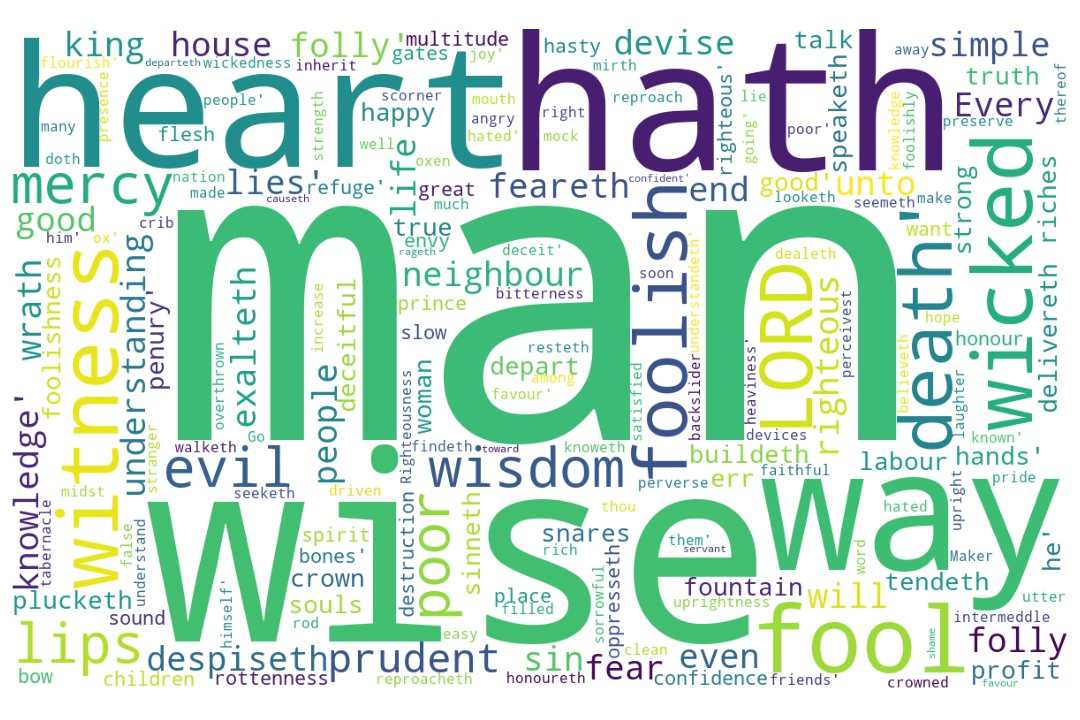
\includegraphics[width=\linewidth]{20OT-Proverbs/Proverb14-WordCloud.jpg}
  \caption{Proverb 14 Word Cloud}
  \label{fig:Proverb 14 Word Cloud}
\end{figure}

\marginpar{\scriptsize \centering \fcolorbox{bone}{lime}{\textbf{WHAT A FOOL DOES}}\\ (Proverbs 14:1-35) \begin{compactenum}[I.][8]
    \item \textbf{Derides Righteousness} (Proverbs 14:9 --  verse with 13 words) \index[scripture]{Proverbs!Pro 14:09}(Pro 14:9)
    \item \textbf{Dealeth in Anger} \index[scripture]{Proverbs!Pro 14:17}(Pro 14:17)
    \item \textbf{Despises Good} \index[scripture]{Proverbs!Pro 14:01, 21}(Pro 14:1, 21)
    \item \textbf{Devises Evil} \index[scripture]{Proverbs!Pro 14:22}(Pro 14:22)
    \item \textbf{Deceives Souls} \index[scripture]{Proverbs!Pro 14:25}(Pro 14:25)
    \item \textbf{Destroys Order} \index[scripture]{Proverbs!Pro 14:28}(Pro 14:28)
    \item \textbf{Deserves Destruction} \index[scripture]{Proverbs!Pro 14:35}(Pro 14:35)
\end{compactenum}}

\marginpar{\scriptsize \centering \fcolorbox{bone}{yellow}{\textbf{7 KINDS OF MEN}}\\ (Proverbs 14:1-35) \begin{compactenum}[I.][8]
    \item The \textbf{False} Man \index[scripture]{Proverbs!Pro 14:05}(Pro 14:5)
    \item The \textbf{Faithful} Man \index[scripture]{Proverbs!Pro 14:05}(Pro 14:5)
    \item The \textbf{Foolish} Man \index[scripture]{Proverbs!Pro 14:08} \index[scripture]{Proverbs!Pro 14:09}  \index[scripture]{Proverbs!Pro 14:24} \index[scripture]{Proverbs!Pro 14:33} (Pro 14:8, 9, 24, 33)
    \item The \textbf{Flourishing} Man \index[scripture]{Proverbs!Pro 14:11} \index[scripture]{Proverbs!Pro 14:35} (Pro 14:11, 35)
    \item The \textbf{Fearing} Man \index[scripture]{Proverbs!Pro 14:16} \index[scripture]{Proverbs!Pro 14:27} (Pro 14:16, 27)
    \item The \textbf{Fleshly} Man \index[scripture]{Proverbs!Pro 14:30} (Pro 14:30)
    \item The \textbf{Favoured} Man \index[scripture]{Proverbs!Pro 14:35} (Pro 14:35)
\end{compactenum}}

\footnote{\textcolor[cmyk]{0.99998,1,0,0}{\hyperlink{TOC}{Return to end of Table of Contents.}}}\footnote{\href{https://audiobible.com/bible/proverbs_14.html}{\textcolor[cmyk]{0.99998,1,0,0}{Proverbs Audio}}}\textcolor[cmyk]{0.99998,1,0,0}{Every wise woman buildeth her house: but the \fcolorbox{bone}{lime}{foolish plucketh it down} with her hands.}
[2] \textcolor[cmyk]{0.99998,1,0,0}{He that walketh in his uprightness feareth the LORD: but \emph{he} \emph{that} \emph{is} perverse in his ways despiseth him.}
[3] \textcolor[cmyk]{0.99998,1,0,0}{In the mouth of the foolish \emph{is} a rod of pride: but the lips of the wise shall preserve them.}
[4] \textcolor[cmyk]{0.99998,1,0,0}{Where no oxen \emph{are}, the crib \emph{is} clean: but much increase \emph{is} by the strength of the ox.}
[5] \textcolor[cmyk]{0.99998,1,0,0}{A faithful witness will not lie: but a false witness will utter lies.}
[6] \textcolor[cmyk]{0.99998,1,0,0}{A scorner seeketh wisdom, and \emph{findeth} \emph{it} not: but knowledge \emph{is} easy unto him that \fcolorbox{bone}{MYGOLD}{understandeth}.}
[7] \textcolor[cmyk]{0.99998,1,0,0}{Go from the presence of a foolish man, when thou perceivest not \emph{in} \emph{him} the lips of knowledge.}
[8] \textcolor[cmyk]{0.99998,1,0,0}{The wisdom of the prudent \emph{is} to understand his way: but the folly of fools \emph{is} deceit.}
[9] \textcolor[cmyk]{0.99998,1,0,0}{Fools make a \fcolorbox{bone}{lime}{mock at sin}: but among the righteous \emph{there} \emph{is} favour.}
[10] \textcolor[cmyk]{0.99998,1,0,0}{The heart knoweth his own bitterness; and a stranger doth not intermeddle with his joy.}
[11] \textcolor[cmyk]{0.99998,1,0,0}{The house of the wicked shall be overthrown: but the tabernacle of the upright shall flourish.}
[12] \textcolor[cmyk]{0.99998,1,0,0}{There is a way which seemeth right unto a man, but the end thereof \emph{are} the ways of death.}
[13] \textcolor[cmyk]{0.99998,1,0,0}{Even in laughter the heart is sorrowful; and the end of that mirth \emph{is} heaviness.}
[14] \textcolor[cmyk]{0.99998,1,0,0}{The backslider in heart shall be filled with his own ways: and a good man \emph{shall} \emph{be} \emph{satisfied} from himself.}
[15] \textcolor[cmyk]{0.99998,1,0,0}{The simple believeth every word: but the prudent \emph{man} looketh well to his going.}
[16] \textcolor[cmyk]{0.99998,1,0,0}{A wise \emph{man} feareth, and departeth from evil: but the fool rageth, and is confident.}
[17] \textcolor[cmyk]{0.99998,1,0,0}{\emph{He} \emph{that} \emph{is} \fcolorbox{bone}{lime}{soon angry} dealeth foolishly: and a man of wicked devices is hated.}
[18] \textcolor[cmyk]{0.99998,1,0,0}{The simple inherit folly: but the prudent are crowned with knowledge.}
[19] \textcolor[cmyk]{0.99998,1,0,0}{The evil bow before the good; and the wicked at the gates of the righteous.}
[20] \textcolor[cmyk]{0.99998,1,0,0}{The poor is hated even of his own neighbour: but the rich \emph{hath} many friends.}
[21] \textcolor[cmyk]{0.99998,1,0,0}{He that \fcolorbox{bone}{lime}{despiseth his neighbour} sinneth: but he that hath mercy on the poor, happy \emph{is} he.}
[22] \textcolor[cmyk]{0.99998,1,0,0}{Do they not err that \fcolorbox{bone}{lime}{devise evil}? but mercy and truth \emph{shall} \emph{be} to them that devise good.}
[23] \textcolor[cmyk]{0.99998,1,0,0}{In all labour there is profit: but the talk of the lips \emph{tendeth} only to penury.}
[24] \textcolor[cmyk]{0.99998,1,0,0}{The crown of the wise \emph{is} their riches: \emph{but} the foolishness of fools \emph{is} folly.}
[25] \textcolor[cmyk]{0.99998,1,0,0}{A true witness delivereth souls: but a \fcolorbox{bone}{lime}{deceitful \emph{witness}} speaketh lies.}
[26] \textcolor[cmyk]{0.99998,1,0,0}{In the fear of the LORD \emph{is} strong confidence: and his children shall have a place of refuge.}
[27] \textcolor[cmyk]{0.99998,1,0,0}{The fear of the LORD \emph{is} a fountain of life, to depart from the snares of death.}
[28] \textcolor[cmyk]{0.99998,1,0,0}{In the multitude of people \emph{is} the king's honour: but in the want of people \emph{is} the \fcolorbox{bone}{lime}{destruction of the prince}.}
[29] \textcolor[cmyk]{0.99998,1,0,0}{\emph{He} \emph{that} \emph{is} slow to wrath \emph{is} of great \fcolorbox{bone}{MYGOLD}{understanding}: but \emph{he} \emph{that} \emph{is} hasty of spirit exalteth folly.}
[30] \textcolor[cmyk]{0.99998,1,0,0}{A sound heart \emph{is} the life of the flesh: but envy the rottenness of the bones.}
[31] \textcolor[cmyk]{0.99998,1,0,0}{He that oppresseth the poor reproacheth his Maker: but he that honoureth him hath mercy on the poor.}
[32] \textcolor[cmyk]{0.99998,1,0,0}{The wicked is driven away in his wickedness: but the righteous hath hope in his death.}
[33] \textcolor[cmyk]{0.99998,1,0,0}{Wisdom resteth in the heart of him that hath \fcolorbox{bone}{MYGOLD}{understanding}: but \emph{that} \emph{which} \emph{is} in the midst of fools is made known.}
[34] \textcolor[cmyk]{0.99998,1,0,0}{\fcolorbox{bone}{MYGOLD}{Righteousness} exalteth a nation: but sin \emph{is} a reproach to any people.}
[35] \textcolor[cmyk]{0.99998,1,0,0}{The king's favour \emph{is} toward a wise servant: but his \fcolorbox{bone}{lime}{wrath is \emph{against}} him that causeth shame.}



\index[NWIV]{15!Proverbs!Pro 14:1}\index[AWIP]{Every!Proverbs!Pro 14:1}\index[AWIP]{wise!Proverbs!Pro 14:1}\index[AWIP]{woman!Proverbs!Pro 14:1}\index[AWIP]{buildeth!Proverbs!Pro 14:1}\index[AWIP]{her!Proverbs!Pro 14:1}\index[AWIP]{her!Proverbs!Pro 14:1 (2)}\index[AWIP]{house!Proverbs!Pro 14:1}\index[AWIP]{but!Proverbs!Pro 14:1}\index[AWIP]{the!Proverbs!Pro 14:1}\index[AWIP]{foolish!Proverbs!Pro 14:1}\index[AWIP]{plucketh!Proverbs!Pro 14:1}\index[AWIP]{it!Proverbs!Pro 14:1}\index[AWIP]{down!Proverbs!Pro 14:1}\index[AWIP]{with!Proverbs!Pro 14:1}\index[AWIP]{hands!Proverbs!Pro 14:1}

\index[NWIV]{19!Proverbs!Pro 14:2}\index[AWIP]{He!Proverbs!Pro 14:2}\index[AWIP]{that!Proverbs!Pro 14:2}\index[AWIP]{walketh!Proverbs!Pro 14:2}\index[AWIP]{in!Proverbs!Pro 14:2}\index[AWIP]{in!Proverbs!Pro 14:2 (2)}\index[AWIP]{his!Proverbs!Pro 14:2}\index[AWIP]{his!Proverbs!Pro 14:2 (2)}\index[AWIP]{uprightness!Proverbs!Pro 14:2}\index[AWIP]{feareth!Proverbs!Pro 14:2}\index[AWIP]{the!Proverbs!Pro 14:2}\index[AWIP]{LORD!Proverbs!Pro 14:2}\index[AWIP]{but!Proverbs!Pro 14:2}\index[AWIP]{\emph{he}!Proverbs!Pro 14:2}\index[AWIP]{\emph{that}!Proverbs!Pro 14:2}\index[AWIP]{\emph{is}!Proverbs!Pro 14:2}\index[AWIP]{perverse!Proverbs!Pro 14:2}\index[AWIP]{ways!Proverbs!Pro 14:2}\index[AWIP]{despiseth!Proverbs!Pro 14:2}\index[AWIP]{him!Proverbs!Pro 14:2}\index[AWIP]{\emph{he}!Proverbs!Pro 14:2}\index[AWIP]{\emph{that}!Proverbs!Pro 14:2}\index[AWIP]{\emph{is}!Proverbs!Pro 14:2}

\index[NWIV]{20!Proverbs!Pro 14:3}\index[AWIP]{In!Proverbs!Pro 14:3}\index[AWIP]{the!Proverbs!Pro 14:3}\index[AWIP]{the!Proverbs!Pro 14:3 (2)}\index[AWIP]{the!Proverbs!Pro 14:3 (3)}\index[AWIP]{the!Proverbs!Pro 14:3 (4)}\index[AWIP]{mouth!Proverbs!Pro 14:3}\index[AWIP]{of!Proverbs!Pro 14:3}\index[AWIP]{of!Proverbs!Pro 14:3 (2)}\index[AWIP]{of!Proverbs!Pro 14:3 (3)}\index[AWIP]{foolish!Proverbs!Pro 14:3}\index[AWIP]{\emph{is}!Proverbs!Pro 14:3}\index[AWIP]{a!Proverbs!Pro 14:3}\index[AWIP]{rod!Proverbs!Pro 14:3}\index[AWIP]{pride!Proverbs!Pro 14:3}\index[AWIP]{but!Proverbs!Pro 14:3}\index[AWIP]{lips!Proverbs!Pro 14:3}\index[AWIP]{wise!Proverbs!Pro 14:3}\index[AWIP]{shall!Proverbs!Pro 14:3}\index[AWIP]{preserve!Proverbs!Pro 14:3}\index[AWIP]{them!Proverbs!Pro 14:3}\index[AWIP]{\emph{is}!Proverbs!Pro 14:3}

\index[NWIV]{18!Proverbs!Pro 14:4}\index[AWIP]{Where!Proverbs!Pro 14:4}\index[AWIP]{no!Proverbs!Pro 14:4}\index[AWIP]{oxen!Proverbs!Pro 14:4}\index[AWIP]{\emph{are}!Proverbs!Pro 14:4}\index[AWIP]{the!Proverbs!Pro 14:4}\index[AWIP]{the!Proverbs!Pro 14:4 (2)}\index[AWIP]{the!Proverbs!Pro 14:4 (3)}\index[AWIP]{crib!Proverbs!Pro 14:4}\index[AWIP]{\emph{is}!Proverbs!Pro 14:4}\index[AWIP]{\emph{is}!Proverbs!Pro 14:4 (2)}\index[AWIP]{clean!Proverbs!Pro 14:4}\index[AWIP]{but!Proverbs!Pro 14:4}\index[AWIP]{much!Proverbs!Pro 14:4}\index[AWIP]{increase!Proverbs!Pro 14:4}\index[AWIP]{by!Proverbs!Pro 14:4}\index[AWIP]{strength!Proverbs!Pro 14:4}\index[AWIP]{of!Proverbs!Pro 14:4}\index[AWIP]{ox!Proverbs!Pro 14:4}\index[AWIP]{\emph{are}!Proverbs!Pro 14:4}\index[AWIP]{\emph{is}!Proverbs!Pro 14:4}\index[AWIP]{\emph{is}!Proverbs!Pro 14:4 (2)}

\index[NWIV]{13!Proverbs!Pro 14:5}\index[AWIP]{A!Proverbs!Pro 14:5}\index[AWIP]{faithful!Proverbs!Pro 14:5}\index[AWIP]{witness!Proverbs!Pro 14:5}\index[AWIP]{witness!Proverbs!Pro 14:5 (2)}\index[AWIP]{will!Proverbs!Pro 14:5}\index[AWIP]{will!Proverbs!Pro 14:5 (2)}\index[AWIP]{not!Proverbs!Pro 14:5}\index[AWIP]{lie!Proverbs!Pro 14:5}\index[AWIP]{but!Proverbs!Pro 14:5}\index[AWIP]{a!Proverbs!Pro 14:5}\index[AWIP]{false!Proverbs!Pro 14:5}\index[AWIP]{utter!Proverbs!Pro 14:5}\index[AWIP]{lies!Proverbs!Pro 14:5}

\index[NWIV]{16!Proverbs!Pro 14:6}\index[AWIP]{A!Proverbs!Pro 14:6}\index[AWIP]{scorner!Proverbs!Pro 14:6}\index[AWIP]{seeketh!Proverbs!Pro 14:6}\index[AWIP]{wisdom!Proverbs!Pro 14:6}\index[AWIP]{and!Proverbs!Pro 14:6}\index[AWIP]{\emph{findeth}!Proverbs!Pro 14:6}\index[AWIP]{\emph{it}!Proverbs!Pro 14:6}\index[AWIP]{not!Proverbs!Pro 14:6}\index[AWIP]{but!Proverbs!Pro 14:6}\index[AWIP]{knowledge!Proverbs!Pro 14:6}\index[AWIP]{\emph{is}!Proverbs!Pro 14:6}\index[AWIP]{easy!Proverbs!Pro 14:6}\index[AWIP]{unto!Proverbs!Pro 14:6}\index[AWIP]{him!Proverbs!Pro 14:6}\index[AWIP]{that!Proverbs!Pro 14:6}\index[AWIP]{understandeth!Proverbs!Pro 14:6}\index[AWIP]{\emph{findeth}!Proverbs!Pro 14:6}\index[AWIP]{\emph{it}!Proverbs!Pro 14:6}\index[AWIP]{\emph{is}!Proverbs!Pro 14:6}

\index[NWIV]{18!Proverbs!Pro 14:7}\index[AWIP]{Go!Proverbs!Pro 14:7}\index[AWIP]{from!Proverbs!Pro 14:7}\index[AWIP]{the!Proverbs!Pro 14:7}\index[AWIP]{the!Proverbs!Pro 14:7 (2)}\index[AWIP]{presence!Proverbs!Pro 14:7}\index[AWIP]{of!Proverbs!Pro 14:7}\index[AWIP]{of!Proverbs!Pro 14:7 (2)}\index[AWIP]{a!Proverbs!Pro 14:7}\index[AWIP]{foolish!Proverbs!Pro 14:7}\index[AWIP]{man!Proverbs!Pro 14:7}\index[AWIP]{when!Proverbs!Pro 14:7}\index[AWIP]{thou!Proverbs!Pro 14:7}\index[AWIP]{perceivest!Proverbs!Pro 14:7}\index[AWIP]{not!Proverbs!Pro 14:7}\index[AWIP]{\emph{in}!Proverbs!Pro 14:7}\index[AWIP]{\emph{him}!Proverbs!Pro 14:7}\index[AWIP]{lips!Proverbs!Pro 14:7}\index[AWIP]{knowledge!Proverbs!Pro 14:7}\index[AWIP]{\emph{in}!Proverbs!Pro 14:7}\index[AWIP]{\emph{him}!Proverbs!Pro 14:7}

\index[NWIV]{17!Proverbs!Pro 14:8}\index[AWIP]{The!Proverbs!Pro 14:8}\index[AWIP]{wisdom!Proverbs!Pro 14:8}\index[AWIP]{of!Proverbs!Pro 14:8}\index[AWIP]{of!Proverbs!Pro 14:8 (2)}\index[AWIP]{the!Proverbs!Pro 14:8}\index[AWIP]{the!Proverbs!Pro 14:8 (2)}\index[AWIP]{prudent!Proverbs!Pro 14:8}\index[AWIP]{\emph{is}!Proverbs!Pro 14:8}\index[AWIP]{\emph{is}!Proverbs!Pro 14:8 (2)}\index[AWIP]{to!Proverbs!Pro 14:8}\index[AWIP]{understand!Proverbs!Pro 14:8}\index[AWIP]{his!Proverbs!Pro 14:8}\index[AWIP]{way!Proverbs!Pro 14:8}\index[AWIP]{but!Proverbs!Pro 14:8}\index[AWIP]{folly!Proverbs!Pro 14:8}\index[AWIP]{fools!Proverbs!Pro 14:8}\index[AWIP]{deceit!Proverbs!Pro 14:8}\index[AWIP]{\emph{is}!Proverbs!Pro 14:8}\index[AWIP]{\emph{is}!Proverbs!Pro 14:8 (2)}

\index[NWIV]{13!Proverbs!Pro 14:9}\index[AWIP]{Fools!Proverbs!Pro 14:9}\index[AWIP]{make!Proverbs!Pro 14:9}\index[AWIP]{a!Proverbs!Pro 14:9}\index[AWIP]{mock!Proverbs!Pro 14:9}\index[AWIP]{at!Proverbs!Pro 14:9}\index[AWIP]{sin!Proverbs!Pro 14:9}\index[AWIP]{but!Proverbs!Pro 14:9}\index[AWIP]{among!Proverbs!Pro 14:9}\index[AWIP]{the!Proverbs!Pro 14:9}\index[AWIP]{righteous!Proverbs!Pro 14:9}\index[AWIP]{\emph{there}!Proverbs!Pro 14:9}\index[AWIP]{\emph{is}!Proverbs!Pro 14:9}\index[AWIP]{favour!Proverbs!Pro 14:9}\index[AWIP]{\emph{there}!Proverbs!Pro 14:9}\index[AWIP]{\emph{is}!Proverbs!Pro 14:9}

\index[NWIV]{15!Proverbs!Pro 14:10}\index[AWIP]{The!Proverbs!Pro 14:10}\index[AWIP]{heart!Proverbs!Pro 14:10}\index[AWIP]{knoweth!Proverbs!Pro 14:10}\index[AWIP]{his!Proverbs!Pro 14:10}\index[AWIP]{his!Proverbs!Pro 14:10 (2)}\index[AWIP]{own!Proverbs!Pro 14:10}\index[AWIP]{bitterness!Proverbs!Pro 14:10}\index[AWIP]{and!Proverbs!Pro 14:10}\index[AWIP]{a!Proverbs!Pro 14:10}\index[AWIP]{stranger!Proverbs!Pro 14:10}\index[AWIP]{doth!Proverbs!Pro 14:10}\index[AWIP]{not!Proverbs!Pro 14:10}\index[AWIP]{intermeddle!Proverbs!Pro 14:10}\index[AWIP]{with!Proverbs!Pro 14:10}\index[AWIP]{joy!Proverbs!Pro 14:10}

\index[NWIV]{16!Proverbs!Pro 14:11}\index[AWIP]{The!Proverbs!Pro 14:11}\index[AWIP]{house!Proverbs!Pro 14:11}\index[AWIP]{of!Proverbs!Pro 14:11}\index[AWIP]{of!Proverbs!Pro 14:11 (2)}\index[AWIP]{the!Proverbs!Pro 14:11}\index[AWIP]{the!Proverbs!Pro 14:11 (2)}\index[AWIP]{the!Proverbs!Pro 14:11 (3)}\index[AWIP]{wicked!Proverbs!Pro 14:11}\index[AWIP]{shall!Proverbs!Pro 14:11}\index[AWIP]{shall!Proverbs!Pro 14:11 (2)}\index[AWIP]{be!Proverbs!Pro 14:11}\index[AWIP]{overthrown!Proverbs!Pro 14:11}\index[AWIP]{but!Proverbs!Pro 14:11}\index[AWIP]{tabernacle!Proverbs!Pro 14:11}\index[AWIP]{upright!Proverbs!Pro 14:11}\index[AWIP]{flourish!Proverbs!Pro 14:11}

\index[NWIV]{19!Proverbs!Pro 14:12}\index[AWIP]{There!Proverbs!Pro 14:12}\index[AWIP]{is!Proverbs!Pro 14:12}\index[AWIP]{a!Proverbs!Pro 14:12}\index[AWIP]{a!Proverbs!Pro 14:12 (2)}\index[AWIP]{way!Proverbs!Pro 14:12}\index[AWIP]{which!Proverbs!Pro 14:12}\index[AWIP]{seemeth!Proverbs!Pro 14:12}\index[AWIP]{right!Proverbs!Pro 14:12}\index[AWIP]{unto!Proverbs!Pro 14:12}\index[AWIP]{man!Proverbs!Pro 14:12}\index[AWIP]{but!Proverbs!Pro 14:12}\index[AWIP]{the!Proverbs!Pro 14:12}\index[AWIP]{the!Proverbs!Pro 14:12 (2)}\index[AWIP]{end!Proverbs!Pro 14:12}\index[AWIP]{thereof!Proverbs!Pro 14:12}\index[AWIP]{\emph{are}!Proverbs!Pro 14:12}\index[AWIP]{ways!Proverbs!Pro 14:12}\index[AWIP]{of!Proverbs!Pro 14:12}\index[AWIP]{death!Proverbs!Pro 14:12}\index[AWIP]{\emph{are}!Proverbs!Pro 14:12}

\index[NWIV]{15!Proverbs!Pro 14:13}\index[AWIP]{Even!Proverbs!Pro 14:13}\index[AWIP]{in!Proverbs!Pro 14:13}\index[AWIP]{laughter!Proverbs!Pro 14:13}\index[AWIP]{the!Proverbs!Pro 14:13}\index[AWIP]{the!Proverbs!Pro 14:13 (2)}\index[AWIP]{heart!Proverbs!Pro 14:13}\index[AWIP]{is!Proverbs!Pro 14:13}\index[AWIP]{sorrowful!Proverbs!Pro 14:13}\index[AWIP]{and!Proverbs!Pro 14:13}\index[AWIP]{end!Proverbs!Pro 14:13}\index[AWIP]{of!Proverbs!Pro 14:13}\index[AWIP]{that!Proverbs!Pro 14:13}\index[AWIP]{mirth!Proverbs!Pro 14:13}\index[AWIP]{\emph{is}!Proverbs!Pro 14:13}\index[AWIP]{heaviness!Proverbs!Pro 14:13}\index[AWIP]{\emph{is}!Proverbs!Pro 14:13}

\index[NWIV]{20!Proverbs!Pro 14:14}\index[AWIP]{The!Proverbs!Pro 14:14}\index[AWIP]{backslider!Proverbs!Pro 14:14}\index[AWIP]{in!Proverbs!Pro 14:14}\index[AWIP]{heart!Proverbs!Pro 14:14}\index[AWIP]{shall!Proverbs!Pro 14:14}\index[AWIP]{be!Proverbs!Pro 14:14}\index[AWIP]{filled!Proverbs!Pro 14:14}\index[AWIP]{with!Proverbs!Pro 14:14}\index[AWIP]{his!Proverbs!Pro 14:14}\index[AWIP]{own!Proverbs!Pro 14:14}\index[AWIP]{ways!Proverbs!Pro 14:14}\index[AWIP]{and!Proverbs!Pro 14:14}\index[AWIP]{a!Proverbs!Pro 14:14}\index[AWIP]{good!Proverbs!Pro 14:14}\index[AWIP]{man!Proverbs!Pro 14:14}\index[AWIP]{\emph{shall}!Proverbs!Pro 14:14}\index[AWIP]{\emph{be}!Proverbs!Pro 14:14}\index[AWIP]{\emph{satisfied}!Proverbs!Pro 14:14}\index[AWIP]{from!Proverbs!Pro 14:14}\index[AWIP]{himself!Proverbs!Pro 14:14}\index[AWIP]{\emph{shall}!Proverbs!Pro 14:14}\index[AWIP]{\emph{be}!Proverbs!Pro 14:14}\index[AWIP]{\emph{satisfied}!Proverbs!Pro 14:14}

\index[NWIV]{14!Proverbs!Pro 14:15}\index[AWIP]{The!Proverbs!Pro 14:15}\index[AWIP]{simple!Proverbs!Pro 14:15}\index[AWIP]{believeth!Proverbs!Pro 14:15}\index[AWIP]{every!Proverbs!Pro 14:15}\index[AWIP]{word!Proverbs!Pro 14:15}\index[AWIP]{but!Proverbs!Pro 14:15}\index[AWIP]{the!Proverbs!Pro 14:15}\index[AWIP]{prudent!Proverbs!Pro 14:15}\index[AWIP]{\emph{man}!Proverbs!Pro 14:15}\index[AWIP]{looketh!Proverbs!Pro 14:15}\index[AWIP]{well!Proverbs!Pro 14:15}\index[AWIP]{to!Proverbs!Pro 14:15}\index[AWIP]{his!Proverbs!Pro 14:15}\index[AWIP]{going!Proverbs!Pro 14:15}\index[AWIP]{\emph{man}!Proverbs!Pro 14:15}

\index[NWIV]{15!Proverbs!Pro 14:16}\index[AWIP]{A!Proverbs!Pro 14:16}\index[AWIP]{wise!Proverbs!Pro 14:16}\index[AWIP]{\emph{man}!Proverbs!Pro 14:16}\index[AWIP]{feareth!Proverbs!Pro 14:16}\index[AWIP]{and!Proverbs!Pro 14:16}\index[AWIP]{and!Proverbs!Pro 14:16 (2)}\index[AWIP]{departeth!Proverbs!Pro 14:16}\index[AWIP]{from!Proverbs!Pro 14:16}\index[AWIP]{evil!Proverbs!Pro 14:16}\index[AWIP]{but!Proverbs!Pro 14:16}\index[AWIP]{the!Proverbs!Pro 14:16}\index[AWIP]{fool!Proverbs!Pro 14:16}\index[AWIP]{rageth!Proverbs!Pro 14:16}\index[AWIP]{is!Proverbs!Pro 14:16}\index[AWIP]{confident!Proverbs!Pro 14:16}\index[AWIP]{\emph{man}!Proverbs!Pro 14:16}

\index[NWIV]{15!Proverbs!Pro 14:17}\index[AWIP]{\emph{He}!Proverbs!Pro 14:17}\index[AWIP]{\emph{that}!Proverbs!Pro 14:17}\index[AWIP]{\emph{is}!Proverbs!Pro 14:17}\index[AWIP]{soon!Proverbs!Pro 14:17}\index[AWIP]{angry!Proverbs!Pro 14:17}\index[AWIP]{dealeth!Proverbs!Pro 14:17}\index[AWIP]{foolishly!Proverbs!Pro 14:17}\index[AWIP]{and!Proverbs!Pro 14:17}\index[AWIP]{a!Proverbs!Pro 14:17}\index[AWIP]{man!Proverbs!Pro 14:17}\index[AWIP]{of!Proverbs!Pro 14:17}\index[AWIP]{wicked!Proverbs!Pro 14:17}\index[AWIP]{devices!Proverbs!Pro 14:17}\index[AWIP]{is!Proverbs!Pro 14:17}\index[AWIP]{hated!Proverbs!Pro 14:17}\index[AWIP]{\emph{He}!Proverbs!Pro 14:17}\index[AWIP]{\emph{that}!Proverbs!Pro 14:17}\index[AWIP]{\emph{is}!Proverbs!Pro 14:17}

\index[NWIV]{11!Proverbs!Pro 14:18}\index[AWIP]{The!Proverbs!Pro 14:18}\index[AWIP]{simple!Proverbs!Pro 14:18}\index[AWIP]{inherit!Proverbs!Pro 14:18}\index[AWIP]{folly!Proverbs!Pro 14:18}\index[AWIP]{but!Proverbs!Pro 14:18}\index[AWIP]{the!Proverbs!Pro 14:18}\index[AWIP]{prudent!Proverbs!Pro 14:18}\index[AWIP]{are!Proverbs!Pro 14:18}\index[AWIP]{crowned!Proverbs!Pro 14:18}\index[AWIP]{with!Proverbs!Pro 14:18}\index[AWIP]{knowledge!Proverbs!Pro 14:18}

\index[NWIV]{15!Proverbs!Pro 14:19}\index[AWIP]{The!Proverbs!Pro 14:19}\index[AWIP]{evil!Proverbs!Pro 14:19}\index[AWIP]{bow!Proverbs!Pro 14:19}\index[AWIP]{before!Proverbs!Pro 14:19}\index[AWIP]{the!Proverbs!Pro 14:19}\index[AWIP]{the!Proverbs!Pro 14:19 (2)}\index[AWIP]{the!Proverbs!Pro 14:19 (3)}\index[AWIP]{the!Proverbs!Pro 14:19 (4)}\index[AWIP]{good!Proverbs!Pro 14:19}\index[AWIP]{and!Proverbs!Pro 14:19}\index[AWIP]{wicked!Proverbs!Pro 14:19}\index[AWIP]{at!Proverbs!Pro 14:19}\index[AWIP]{gates!Proverbs!Pro 14:19}\index[AWIP]{of!Proverbs!Pro 14:19}\index[AWIP]{righteous!Proverbs!Pro 14:19}

\index[NWIV]{15!Proverbs!Pro 14:20}\index[AWIP]{The!Proverbs!Pro 14:20}\index[AWIP]{poor!Proverbs!Pro 14:20}\index[AWIP]{is!Proverbs!Pro 14:20}\index[AWIP]{hated!Proverbs!Pro 14:20}\index[AWIP]{even!Proverbs!Pro 14:20}\index[AWIP]{of!Proverbs!Pro 14:20}\index[AWIP]{his!Proverbs!Pro 14:20}\index[AWIP]{own!Proverbs!Pro 14:20}\index[AWIP]{neighbour!Proverbs!Pro 14:20}\index[AWIP]{but!Proverbs!Pro 14:20}\index[AWIP]{the!Proverbs!Pro 14:20}\index[AWIP]{rich!Proverbs!Pro 14:20}\index[AWIP]{\emph{hath}!Proverbs!Pro 14:20}\index[AWIP]{many!Proverbs!Pro 14:20}\index[AWIP]{friends!Proverbs!Pro 14:20}\index[AWIP]{\emph{hath}!Proverbs!Pro 14:20}

\index[NWIV]{17!Proverbs!Pro 14:21}\index[AWIP]{He!Proverbs!Pro 14:21}\index[AWIP]{that!Proverbs!Pro 14:21}\index[AWIP]{that!Proverbs!Pro 14:21 (2)}\index[AWIP]{despiseth!Proverbs!Pro 14:21}\index[AWIP]{his!Proverbs!Pro 14:21}\index[AWIP]{neighbour!Proverbs!Pro 14:21}\index[AWIP]{sinneth!Proverbs!Pro 14:21}\index[AWIP]{but!Proverbs!Pro 14:21}\index[AWIP]{he!Proverbs!Pro 14:21}\index[AWIP]{he!Proverbs!Pro 14:21 (2)}\index[AWIP]{hath!Proverbs!Pro 14:21}\index[AWIP]{mercy!Proverbs!Pro 14:21}\index[AWIP]{on!Proverbs!Pro 14:21}\index[AWIP]{the!Proverbs!Pro 14:21}\index[AWIP]{poor!Proverbs!Pro 14:21}\index[AWIP]{happy!Proverbs!Pro 14:21}\index[AWIP]{\emph{is}!Proverbs!Pro 14:21}\index[AWIP]{\emph{is}!Proverbs!Pro 14:21}

\index[NWIV]{18!Proverbs!Pro 14:22}\index[AWIP]{Do!Proverbs!Pro 14:22}\index[AWIP]{they!Proverbs!Pro 14:22}\index[AWIP]{not!Proverbs!Pro 14:22}\index[AWIP]{err!Proverbs!Pro 14:22}\index[AWIP]{that!Proverbs!Pro 14:22}\index[AWIP]{that!Proverbs!Pro 14:22 (2)}\index[AWIP]{devise!Proverbs!Pro 14:22}\index[AWIP]{devise!Proverbs!Pro 14:22 (2)}\index[AWIP]{evil?!Proverbs!Pro 14:22}\index[AWIP]{but!Proverbs!Pro 14:22}\index[AWIP]{mercy!Proverbs!Pro 14:22}\index[AWIP]{and!Proverbs!Pro 14:22}\index[AWIP]{truth!Proverbs!Pro 14:22}\index[AWIP]{\emph{shall}!Proverbs!Pro 14:22}\index[AWIP]{\emph{be}!Proverbs!Pro 14:22}\index[AWIP]{to!Proverbs!Pro 14:22}\index[AWIP]{them!Proverbs!Pro 14:22}\index[AWIP]{good!Proverbs!Pro 14:22}\index[AWIP]{\emph{shall}!Proverbs!Pro 14:22}\index[AWIP]{\emph{be}!Proverbs!Pro 14:22}

\index[NWIV]{16!Proverbs!Pro 14:23}\index[AWIP]{In!Proverbs!Pro 14:23}\index[AWIP]{all!Proverbs!Pro 14:23}\index[AWIP]{labour!Proverbs!Pro 14:23}\index[AWIP]{there!Proverbs!Pro 14:23}\index[AWIP]{is!Proverbs!Pro 14:23}\index[AWIP]{profit!Proverbs!Pro 14:23}\index[AWIP]{but!Proverbs!Pro 14:23}\index[AWIP]{the!Proverbs!Pro 14:23}\index[AWIP]{the!Proverbs!Pro 14:23 (2)}\index[AWIP]{talk!Proverbs!Pro 14:23}\index[AWIP]{of!Proverbs!Pro 14:23}\index[AWIP]{lips!Proverbs!Pro 14:23}\index[AWIP]{\emph{tendeth}!Proverbs!Pro 14:23}\index[AWIP]{only!Proverbs!Pro 14:23}\index[AWIP]{to!Proverbs!Pro 14:23}\index[AWIP]{penury!Proverbs!Pro 14:23}\index[AWIP]{\emph{tendeth}!Proverbs!Pro 14:23}

\index[NWIV]{15!Proverbs!Pro 14:24}\index[AWIP]{The!Proverbs!Pro 14:24}\index[AWIP]{crown!Proverbs!Pro 14:24}\index[AWIP]{of!Proverbs!Pro 14:24}\index[AWIP]{of!Proverbs!Pro 14:24 (2)}\index[AWIP]{the!Proverbs!Pro 14:24}\index[AWIP]{the!Proverbs!Pro 14:24 (2)}\index[AWIP]{wise!Proverbs!Pro 14:24}\index[AWIP]{\emph{is}!Proverbs!Pro 14:24}\index[AWIP]{\emph{is}!Proverbs!Pro 14:24 (2)}\index[AWIP]{their!Proverbs!Pro 14:24}\index[AWIP]{riches!Proverbs!Pro 14:24}\index[AWIP]{\emph{but}!Proverbs!Pro 14:24}\index[AWIP]{foolishness!Proverbs!Pro 14:24}\index[AWIP]{fools!Proverbs!Pro 14:24}\index[AWIP]{folly!Proverbs!Pro 14:24}\index[AWIP]{\emph{is}!Proverbs!Pro 14:24}\index[AWIP]{\emph{is}!Proverbs!Pro 14:24 (2)}\index[AWIP]{\emph{but}!Proverbs!Pro 14:24}

\index[NWIV]{11!Proverbs!Pro 14:25}\index[AWIP]{A!Proverbs!Pro 14:25}\index[AWIP]{true!Proverbs!Pro 14:25}\index[AWIP]{witness!Proverbs!Pro 14:25}\index[AWIP]{delivereth!Proverbs!Pro 14:25}\index[AWIP]{souls!Proverbs!Pro 14:25}\index[AWIP]{but!Proverbs!Pro 14:25}\index[AWIP]{a!Proverbs!Pro 14:25}\index[AWIP]{deceitful!Proverbs!Pro 14:25}\index[AWIP]{\emph{witness}!Proverbs!Pro 14:25}\index[AWIP]{speaketh!Proverbs!Pro 14:25}\index[AWIP]{lies!Proverbs!Pro 14:25}\index[AWIP]{\emph{witness}!Proverbs!Pro 14:25}

\index[NWIV]{18!Proverbs!Pro 14:26}\index[AWIP]{In!Proverbs!Pro 14:26}\index[AWIP]{the!Proverbs!Pro 14:26}\index[AWIP]{the!Proverbs!Pro 14:26 (2)}\index[AWIP]{fear!Proverbs!Pro 14:26}\index[AWIP]{of!Proverbs!Pro 14:26}\index[AWIP]{of!Proverbs!Pro 14:26 (2)}\index[AWIP]{LORD!Proverbs!Pro 14:26}\index[AWIP]{\emph{is}!Proverbs!Pro 14:26}\index[AWIP]{strong!Proverbs!Pro 14:26}\index[AWIP]{confidence!Proverbs!Pro 14:26}\index[AWIP]{and!Proverbs!Pro 14:26}\index[AWIP]{his!Proverbs!Pro 14:26}\index[AWIP]{children!Proverbs!Pro 14:26}\index[AWIP]{shall!Proverbs!Pro 14:26}\index[AWIP]{have!Proverbs!Pro 14:26}\index[AWIP]{a!Proverbs!Pro 14:26}\index[AWIP]{place!Proverbs!Pro 14:26}\index[AWIP]{refuge!Proverbs!Pro 14:26}\index[AWIP]{\emph{is}!Proverbs!Pro 14:26}

\index[NWIV]{17!Proverbs!Pro 14:27}\index[AWIP]{The!Proverbs!Pro 14:27}\index[AWIP]{fear!Proverbs!Pro 14:27}\index[AWIP]{of!Proverbs!Pro 14:27}\index[AWIP]{of!Proverbs!Pro 14:27 (2)}\index[AWIP]{of!Proverbs!Pro 14:27 (3)}\index[AWIP]{the!Proverbs!Pro 14:27}\index[AWIP]{the!Proverbs!Pro 14:27 (2)}\index[AWIP]{LORD!Proverbs!Pro 14:27}\index[AWIP]{\emph{is}!Proverbs!Pro 14:27}\index[AWIP]{a!Proverbs!Pro 14:27}\index[AWIP]{fountain!Proverbs!Pro 14:27}\index[AWIP]{life!Proverbs!Pro 14:27}\index[AWIP]{to!Proverbs!Pro 14:27}\index[AWIP]{depart!Proverbs!Pro 14:27}\index[AWIP]{from!Proverbs!Pro 14:27}\index[AWIP]{snares!Proverbs!Pro 14:27}\index[AWIP]{death!Proverbs!Pro 14:27}\index[AWIP]{\emph{is}!Proverbs!Pro 14:27}

\index[NWIV]{21!Proverbs!Pro 14:28}\index[AWIP]{In!Proverbs!Pro 14:28}\index[AWIP]{the!Proverbs!Pro 14:28}\index[AWIP]{the!Proverbs!Pro 14:28 (2)}\index[AWIP]{the!Proverbs!Pro 14:28 (3)}\index[AWIP]{the!Proverbs!Pro 14:28 (4)}\index[AWIP]{the!Proverbs!Pro 14:28 (5)}\index[AWIP]{multitude!Proverbs!Pro 14:28}\index[AWIP]{of!Proverbs!Pro 14:28}\index[AWIP]{of!Proverbs!Pro 14:28 (2)}\index[AWIP]{of!Proverbs!Pro 14:28 (3)}\index[AWIP]{people!Proverbs!Pro 14:28}\index[AWIP]{people!Proverbs!Pro 14:28 (2)}\index[AWIP]{\emph{is}!Proverbs!Pro 14:28}\index[AWIP]{\emph{is}!Proverbs!Pro 14:28 (2)}\index[AWIP]{king's!Proverbs!Pro 14:28}\index[AWIP]{honour!Proverbs!Pro 14:28}\index[AWIP]{but!Proverbs!Pro 14:28}\index[AWIP]{in!Proverbs!Pro 14:28}\index[AWIP]{want!Proverbs!Pro 14:28}\index[AWIP]{destruction!Proverbs!Pro 14:28}\index[AWIP]{prince!Proverbs!Pro 14:28}\index[AWIP]{\emph{is}!Proverbs!Pro 14:28}\index[AWIP]{\emph{is}!Proverbs!Pro 14:28 (2)}

\index[NWIV]{19!Proverbs!Pro 14:29}\index[AWIP]{\emph{He}!Proverbs!Pro 14:29}\index[AWIP]{\emph{that}!Proverbs!Pro 14:29}\index[AWIP]{\emph{that}!Proverbs!Pro 14:29 (2)}\index[AWIP]{\emph{is}!Proverbs!Pro 14:29}\index[AWIP]{\emph{is}!Proverbs!Pro 14:29 (2)}\index[AWIP]{\emph{is}!Proverbs!Pro 14:29 (3)}\index[AWIP]{slow!Proverbs!Pro 14:29}\index[AWIP]{to!Proverbs!Pro 14:29}\index[AWIP]{wrath!Proverbs!Pro 14:29}\index[AWIP]{of!Proverbs!Pro 14:29}\index[AWIP]{of!Proverbs!Pro 14:29 (2)}\index[AWIP]{great!Proverbs!Pro 14:29}\index[AWIP]{understanding!Proverbs!Pro 14:29}\index[AWIP]{but!Proverbs!Pro 14:29}\index[AWIP]{\emph{he}!Proverbs!Pro 14:29}\index[AWIP]{hasty!Proverbs!Pro 14:29}\index[AWIP]{spirit!Proverbs!Pro 14:29}\index[AWIP]{exalteth!Proverbs!Pro 14:29}\index[AWIP]{folly!Proverbs!Pro 14:29}\index[AWIP]{\emph{He}!Proverbs!Pro 14:29}\index[AWIP]{\emph{that}!Proverbs!Pro 14:29}\index[AWIP]{\emph{that}!Proverbs!Pro 14:29 (2)}\index[AWIP]{\emph{is}!Proverbs!Pro 14:29}\index[AWIP]{\emph{is}!Proverbs!Pro 14:29 (2)}\index[AWIP]{\emph{is}!Proverbs!Pro 14:29 (3)}\index[AWIP]{\emph{he}!Proverbs!Pro 14:29}

\index[NWIV]{16!Proverbs!Pro 14:30}\index[AWIP]{A!Proverbs!Pro 14:30}\index[AWIP]{sound!Proverbs!Pro 14:30}\index[AWIP]{heart!Proverbs!Pro 14:30}\index[AWIP]{\emph{is}!Proverbs!Pro 14:30}\index[AWIP]{the!Proverbs!Pro 14:30}\index[AWIP]{the!Proverbs!Pro 14:30 (2)}\index[AWIP]{the!Proverbs!Pro 14:30 (3)}\index[AWIP]{the!Proverbs!Pro 14:30 (4)}\index[AWIP]{life!Proverbs!Pro 14:30}\index[AWIP]{of!Proverbs!Pro 14:30}\index[AWIP]{of!Proverbs!Pro 14:30 (2)}\index[AWIP]{flesh!Proverbs!Pro 14:30}\index[AWIP]{but!Proverbs!Pro 14:30}\index[AWIP]{envy!Proverbs!Pro 14:30}\index[AWIP]{rottenness!Proverbs!Pro 14:30}\index[AWIP]{bones!Proverbs!Pro 14:30}\index[AWIP]{\emph{is}!Proverbs!Pro 14:30}

\index[NWIV]{18!Proverbs!Pro 14:31}\index[AWIP]{He!Proverbs!Pro 14:31}\index[AWIP]{that!Proverbs!Pro 14:31}\index[AWIP]{that!Proverbs!Pro 14:31 (2)}\index[AWIP]{oppresseth!Proverbs!Pro 14:31}\index[AWIP]{the!Proverbs!Pro 14:31}\index[AWIP]{the!Proverbs!Pro 14:31 (2)}\index[AWIP]{poor!Proverbs!Pro 14:31}\index[AWIP]{poor!Proverbs!Pro 14:31 (2)}\index[AWIP]{reproacheth!Proverbs!Pro 14:31}\index[AWIP]{his!Proverbs!Pro 14:31}\index[AWIP]{Maker!Proverbs!Pro 14:31}\index[AWIP]{but!Proverbs!Pro 14:31}\index[AWIP]{he!Proverbs!Pro 14:31}\index[AWIP]{honoureth!Proverbs!Pro 14:31}\index[AWIP]{him!Proverbs!Pro 14:31}\index[AWIP]{hath!Proverbs!Pro 14:31}\index[AWIP]{mercy!Proverbs!Pro 14:31}\index[AWIP]{on!Proverbs!Pro 14:31}

\index[NWIV]{16!Proverbs!Pro 14:32}\index[AWIP]{The!Proverbs!Pro 14:32}\index[AWIP]{wicked!Proverbs!Pro 14:32}\index[AWIP]{is!Proverbs!Pro 14:32}\index[AWIP]{driven!Proverbs!Pro 14:32}\index[AWIP]{away!Proverbs!Pro 14:32}\index[AWIP]{in!Proverbs!Pro 14:32}\index[AWIP]{in!Proverbs!Pro 14:32 (2)}\index[AWIP]{his!Proverbs!Pro 14:32}\index[AWIP]{his!Proverbs!Pro 14:32 (2)}\index[AWIP]{wickedness!Proverbs!Pro 14:32}\index[AWIP]{but!Proverbs!Pro 14:32}\index[AWIP]{the!Proverbs!Pro 14:32}\index[AWIP]{righteous!Proverbs!Pro 14:32}\index[AWIP]{hath!Proverbs!Pro 14:32}\index[AWIP]{hope!Proverbs!Pro 14:32}\index[AWIP]{death!Proverbs!Pro 14:32}

\index[NWIV]{22!Proverbs!Pro 14:33}\index[AWIP]{Wisdom!Proverbs!Pro 14:33}\index[AWIP]{resteth!Proverbs!Pro 14:33}\index[AWIP]{in!Proverbs!Pro 14:33}\index[AWIP]{in!Proverbs!Pro 14:33 (2)}\index[AWIP]{the!Proverbs!Pro 14:33}\index[AWIP]{the!Proverbs!Pro 14:33 (2)}\index[AWIP]{heart!Proverbs!Pro 14:33}\index[AWIP]{of!Proverbs!Pro 14:33}\index[AWIP]{of!Proverbs!Pro 14:33 (2)}\index[AWIP]{him!Proverbs!Pro 14:33}\index[AWIP]{that!Proverbs!Pro 14:33}\index[AWIP]{hath!Proverbs!Pro 14:33}\index[AWIP]{understanding!Proverbs!Pro 14:33}\index[AWIP]{but!Proverbs!Pro 14:33}\index[AWIP]{\emph{that}!Proverbs!Pro 14:33}\index[AWIP]{\emph{which}!Proverbs!Pro 14:33}\index[AWIP]{\emph{is}!Proverbs!Pro 14:33}\index[AWIP]{midst!Proverbs!Pro 14:33}\index[AWIP]{fools!Proverbs!Pro 14:33}\index[AWIP]{is!Proverbs!Pro 14:33}\index[AWIP]{made!Proverbs!Pro 14:33}\index[AWIP]{known!Proverbs!Pro 14:33}\index[AWIP]{\emph{that}!Proverbs!Pro 14:33}\index[AWIP]{\emph{which}!Proverbs!Pro 14:33}\index[AWIP]{\emph{is}!Proverbs!Pro 14:33}

\index[NWIV]{12!Proverbs!Pro 14:34}\index[AWIP]{Righteousness!Proverbs!Pro 14:34}\index[AWIP]{exalteth!Proverbs!Pro 14:34}\index[AWIP]{a!Proverbs!Pro 14:34}\index[AWIP]{a!Proverbs!Pro 14:34 (2)}\index[AWIP]{nation!Proverbs!Pro 14:34}\index[AWIP]{but!Proverbs!Pro 14:34}\index[AWIP]{sin!Proverbs!Pro 14:34}\index[AWIP]{\emph{is}!Proverbs!Pro 14:34}\index[AWIP]{reproach!Proverbs!Pro 14:34}\index[AWIP]{to!Proverbs!Pro 14:34}\index[AWIP]{any!Proverbs!Pro 14:34}\index[AWIP]{people!Proverbs!Pro 14:34}\index[AWIP]{\emph{is}!Proverbs!Pro 14:34}

\index[NWIV]{17!Proverbs!Pro 14:35}\index[AWIP]{The!Proverbs!Pro 14:35}\index[AWIP]{king's!Proverbs!Pro 14:35}\index[AWIP]{favour!Proverbs!Pro 14:35}\index[AWIP]{\emph{is}!Proverbs!Pro 14:35}\index[AWIP]{toward!Proverbs!Pro 14:35}\index[AWIP]{a!Proverbs!Pro 14:35}\index[AWIP]{wise!Proverbs!Pro 14:35}\index[AWIP]{servant!Proverbs!Pro 14:35}\index[AWIP]{but!Proverbs!Pro 14:35}\index[AWIP]{his!Proverbs!Pro 14:35}\index[AWIP]{wrath!Proverbs!Pro 14:35}\index[AWIP]{is!Proverbs!Pro 14:35}\index[AWIP]{\emph{against}!Proverbs!Pro 14:35}\index[AWIP]{him!Proverbs!Pro 14:35}\index[AWIP]{that!Proverbs!Pro 14:35}\index[AWIP]{causeth!Proverbs!Pro 14:35}\index[AWIP]{shame!Proverbs!Pro 14:35}\index[AWIP]{\emph{is}!Proverbs!Pro 14:35}\index[AWIP]{\emph{against}!Proverbs!Pro 14:35}

%%%%%%%%%%%%%%%%%%%%%%%%%%%%%%%%%%%

\index[DOCTRINES]{Practicology - Selectivity!Proverbs!Pro 14:7}

\index[DOCTRINES]{Practicology - Self-confidence!Proverbs!Pro 14:16}

\index[DOCTRINES]{Practicology - Self-control!Proverbs!Pro 14:29}

\index[DOCTRINES]{Practicology - Shame!Proverbs!Pro 14:35}






\section{Proverbs 14 Outlines}

\subsection{My Outlines}

\subsubsection{What a Fool Does}
\index[speaker]{Keith Anthony!Proverb 14 (What a Fool Does)}
\index[series]{Proverbs (Keith Anthony)!Pro 14 (What a Fool Does)}
\index[date]{2015/09/12!Proverb 14 (What a Fool Does) (Keith Anthony)}
\begin{compactenum}[I.]
    \item \textbf{Derides Righteousness} (Proverbs 14:9 --  verse with 13 words) \index[scripture]{Proverbs!Pro 14:09}(Pro 14:9)
    \item \textbf{Dealeth in Anger} \index[scripture]{Proverbs!Pro 14:17}(Pro 14:17)
    \item \textbf{Despises Good} \index[scripture]{Proverbs!Pro 14:01, 21}(Pro 14:1, 21)
    \item \textbf{Devises Evil} \index[scripture]{Proverbs!Pro 14:22}(Pro 14:22)
    \item \textbf{Deceives Souls} \index[scripture]{Proverbs!Pro 14:25}(Pro 14:25)
    \item \textbf{Destroys Order} \index[scripture]{Proverbs!Pro 14:28}(Pro 14:28)
    \item \textbf{Deserves Destruction} \index[scripture]{Proverbs!Pro 14:35}(Pro 14:35)
\end{compactenum}

\subsubsection{What the Wise Do}

\index[speaker]{Keith Anthony!Proverb 14 (What the Wise Do)}
\index[series]{Proverbs (Keith Anthony)!Pro 14 (What the Wise Do)}
\index[date]{2016/05/22!Proverb 14 (What the Wise Do) (Keith Anthony)}
\begin{compactenum}[I.]
    \item \textbf{A Wise Woman Builds} \index[scripture]{Proverbs!Pro 14:01}(Pro 14:1)
    \item \textbf{A Walking Man Fears} \index[scripture]{Proverbs!Pro 14:02}(Pro 14:2)
    \item \textbf{A Winsome One Chooses Words} \index[scripture]{Proverbs!Pro 14:03}(Pro 14:3)
    \item \textbf{A Witnessing Person Utters Truth} \index[scripture]{Proverbs!Pro 14:05}(Pro 14:5)
    \item \textbf{A Wary Person Runs from Foolishness} \index[scripture]{Proverbs!Pro 14:07}(Pro 14:7)
    \item \textbf{A Watching Person Gains Knowledge} \index[scripture]{Proverbs!Pro 14:06}(Pro 14:6)
    \item \textbf{A Working Man Profits} \index[scripture]{Proverbs!Pro 14:23}(Pro 14:23)
\end{compactenum}


\subsection{Outlines from others}

\section{Proverb 14 Comments}

\subsection{Numeric Nuggets}
\textbf{13:} Verses 5 and 9 have 13 words. Verses 9 and 28 have 13 unique words. The 13-letter words ``understandeth,'' ``understanding,'' and ``Righteousnes'' are found in the chapter.


\subsection{Proverb 14 Repeated Phrases}


%%%%%%%%%%
%%%%%%%%%%
\normalsize
 
\begin{center}
\begin{longtable}{|c|c|}
\caption[Proverb 14 Repeated Phrases]{Proverb 14 Repeated Phrases}\label{table:Repeated Phrases Proverb 14} \\
\hline \multicolumn{1}{|c|}{\textbf{Phrase}} & \multicolumn{1}{c|}{\textbf{Frequency}} \\ \hline 
\endfirsthead
 
\multicolumn{2}{c}
{{\bfseries \tablename\ \thetable{} -- continued from previous page}} \\  
\hline \multicolumn{1}{|c|}{\textbf{Phrase}} & \multicolumn{1}{c|}{\textbf{Frequency}} \\ \hline 
\endhead
 
\hline \multicolumn{2}{c}{{ }} \\ \hline
\endfoot 
of the & 14\\ \hline 
but the & 11\\ \hline 
in his & 4\\ \hline 
\emph{that} \emph{is} & 4\\ \hline 
He that & 3\\ \hline 
the LORD & 3\\ \hline 
In the & 3\\ \hline 
\emph{is} a & 3\\ \hline 
the lips & 3\\ \hline 
him that & 3\\ \hline 
the prudent & 3\\ \hline 
of fools & 3\\ \hline 
the righteous & 3\\ \hline 
his own & 3\\ \hline 
and a & 3\\ \hline 
the poor & 3\\ \hline 
\emph{is} the & 3\\ \hline 
in the & 3\\ \hline 
\end{longtable}
\end{center}



%%%%%%%%%%
%%%%%%%%%%



%\newpage
\section{Proverb 14 Statistics}

%%%%%%%%%%%%%%%%%%%%%%%%%%%
%%%%% Word Statistics
%%%%%%%%%%%%%%%%%%%%%%%%%%

\normalsize
\subsection{Chapter Word Statistics}


%%%%%%%%%%
%%%%%%%%%%
 
\begin{center}
\begin{longtable}{l|c|c|c|c}
\caption[Stats for Proverb 14]{Stats for Proverb 14} \label{table:Stats for Proverb 14} \\ 
\hline \multicolumn{1}{|c|}{\textbf{Verse(s)}} & \multicolumn{1}{|c|}{\textbf{Count}} & \multicolumn{1}{|c|}{\textbf{Unique}} & \multicolumn{1}{|c|}{\textbf{Italics}} & \multicolumn{1}{|c|}{\textbf{Uniq Italic}}  \\ \hline 
\endfirsthead
 
\multicolumn{5}{c}
{{\bfseries \tablename\ \thetable{} -- continued from previous page}} \\  
\hline \multicolumn{1}{|c|}{\textbf{Verse(s)}} & \multicolumn{1}{|c|}{\textbf{Count}} & \multicolumn{1}{|c|}{\textbf{Unique}} & \multicolumn{1}{|c|}{\textbf{Italics}} & \multicolumn{1}{|c|}{\textbf{Uniq Italic}}  \\ \hline 
\endhead
 
\hline \multicolumn{5}{|r|}{{Continued if needed}} \\ \hline
\endfoot 
1 & 15 & 14 & 0 & 0\\ \hline
2 & 19 & 17 & 3 & 3\\ \hline
3 & 20 & 15 & 1 & 1\\ \hline
4 & 18 & 15 & 3 & 2\\ \hline
5 & 13 & 11 & 0 & 0\\ \hline
6 & 16 & 16 & 3 & 3\\ \hline
7 & 18 & 16 & 2 & 2\\ \hline
8 & 17 & 14 & 2 & 1\\ \hline
9 & 13 & 13 & 2 & 2\\ \hline
10 & 15 & 14 & 0 & 0\\ \hline
11 & 16 & 12 & 0 & 0\\ \hline
12 & 19 & 17 & 1 & 1\\ \hline
13 & 15 & 14 & 1 & 1\\ \hline
14 & 20 & 20 & 3 & 3\\ \hline
15 & 14 & 14 & 1 & 1\\ \hline
16 & 15 & 14 & 1 & 1\\ \hline
17 & 15 & 15 & 3 & 3\\ \hline
18 & 11 & 11 & 0 & 0\\ \hline
19 & 15 & 12 & 0 & 0\\ \hline
20 & 15 & 15 & 1 & 1\\ \hline
21 & 17 & 15 & 1 & 1\\ \hline
22 & 18 & 16 & 2 & 2\\ \hline
23 & 16 & 15 & 1 & 1\\ \hline
24 & 15 & 12 & 3 & 2\\ \hline
25 & 11 & 11 & 1 & 1\\ \hline
26 & 18 & 16 & 1 & 1\\ \hline
27 & 17 & 14 & 1 & 1\\ \hline
28 & 21 & 13 & 2 & 1\\ \hline
29 & 19 & 15 & 7 & 4\\ \hline
30 & 16 & 12 & 1 & 1\\ \hline
31 & 18 & 15 & 0 & 0\\ \hline
32 & 16 & 14 & 0 & 0\\ \hline
33 & 22 & 19 & 3 & 3\\ \hline
34 & 12 & 11 & 1 & 1\\ \hline
35 & 17 & 17 & 2 & 2\\ \hline
\hline \hline
Total & 572 & 245 & 53 & 20




\end{longtable}
\end{center}

%%%%%%%%%%
%%%%%%%%%%


\subsection{Words by Frequency}

\begin{center}
\begin{longtable}{l|r}
\caption[Word Frequencies in Proverb 14]{Word Frequencies in Proverb 14} \label{table:WordsIn-Proverb-14} \\ 
\hline \multicolumn{1}{|c|}{\textbf{Word}} & \multicolumn{1}{c|}{\textbf{Frequency}} \\ \hline 
\endfirsthead
  
\multicolumn{2}{c}  
{{\bfseries \tablename\ \thetable{} -- continued from previous page}} \\   
\hline \multicolumn{1}{|c|}{\textbf{Word}} & \multicolumn{1}{c|}{\textbf{Frequency}} \\ \hline   
\endhead  
  
\hline \multicolumn{2}{|r|}{{Continue}} \\ \hline  
\endfoot  
  
\hline \hline  
\endlastfoot  
  
the & 52\\ \hline 
of & 32\\ \hline 
but & 26\\ \hline 
\emph{is} & 24\\ \hline 
a & 15\\ \hline 
his & 14\\ \hline 
The & 12\\ \hline 
that & 11\\ \hline 
and & 10\\ \hline 
in & 9\\ \hline 
is & 9\\ \hline 
to & 7\\ \hline 
wise & 5\\ \hline 
\emph{that} & 5\\ \hline 
him & 5\\ \hline 
shall & 5\\ \hline 
A & 5\\ \hline 
not & 5\\ \hline 
heart & 5\\ \hline 
with & 4\\ \hline 
In & 4\\ \hline 
from & 4\\ \hline 
man & 4\\ \hline 
folly & 4\\ \hline 
wicked & 4\\ \hline 
poor & 4\\ \hline 
hath & 4\\ \hline 
foolish & 3\\ \hline 
He & 3\\ \hline 
LORD & 3\\ \hline 
ways & 3\\ \hline 
lips & 3\\ \hline 
witness & 3\\ \hline 
knowledge & 3\\ \hline 
prudent & 3\\ \hline 
fools & 3\\ \hline 
righteous & 3\\ \hline 
own & 3\\ \hline 
death & 3\\ \hline 
good & 3\\ \hline 
evil & 3\\ \hline 
he & 3\\ \hline 
mercy & 3\\ \hline 
people & 3\\ \hline 
her & 2\\ \hline 
house & 2\\ \hline 
feareth & 2\\ \hline 
\emph{he} & 2\\ \hline 
despiseth & 2\\ \hline 
them & 2\\ \hline 
\emph{are} & 2\\ \hline 
will & 2\\ \hline 
lies & 2\\ \hline 
wisdom & 2\\ \hline 
unto & 2\\ \hline 
way & 2\\ \hline 
at & 2\\ \hline 
sin & 2\\ \hline 
favour & 2\\ \hline 
be & 2\\ \hline 
end & 2\\ \hline 
\emph{shall} & 2\\ \hline 
\emph{be} & 2\\ \hline 
simple & 2\\ \hline 
\emph{man} & 2\\ \hline 
\emph{He} & 2\\ \hline 
hated & 2\\ \hline 
neighbour & 2\\ \hline 
on & 2\\ \hline 
devise & 2\\ \hline 
fear & 2\\ \hline 
life & 2\\ \hline 
king's & 2\\ \hline 
wrath & 2\\ \hline 
understanding & 2\\ \hline 
exalteth & 2\\ \hline 
Every & 1\\ \hline 
woman & 1\\ \hline 
buildeth & 1\\ \hline 
plucketh & 1\\ \hline 
it & 1\\ \hline 
down & 1\\ \hline 
hands & 1\\ \hline 
walketh & 1\\ \hline 
uprightness & 1\\ \hline 
perverse & 1\\ \hline 
mouth & 1\\ \hline 
rod & 1\\ \hline 
pride & 1\\ \hline 
preserve & 1\\ \hline 
Where & 1\\ \hline 
no & 1\\ \hline 
oxen & 1\\ \hline 
crib & 1\\ \hline 
clean & 1\\ \hline 
much & 1\\ \hline 
increase & 1\\ \hline 
by & 1\\ \hline 
strength & 1\\ \hline 
ox & 1\\ \hline 
faithful & 1\\ \hline 
lie & 1\\ \hline 
false & 1\\ \hline 
utter & 1\\ \hline 
scorner & 1\\ \hline 
seeketh & 1\\ \hline 
\emph{findeth} & 1\\ \hline 
\emph{it} & 1\\ \hline 
easy & 1\\ \hline 
understandeth & 1\\ \hline 
Go & 1\\ \hline 
presence & 1\\ \hline 
when & 1\\ \hline 
thou & 1\\ \hline 
perceivest & 1\\ \hline 
\emph{in} & 1\\ \hline 
\emph{him} & 1\\ \hline 
understand & 1\\ \hline 
deceit & 1\\ \hline 
Fools & 1\\ \hline 
make & 1\\ \hline 
mock & 1\\ \hline 
among & 1\\ \hline 
\emph{there} & 1\\ \hline 
knoweth & 1\\ \hline 
bitterness & 1\\ \hline 
stranger & 1\\ \hline 
doth & 1\\ \hline 
intermeddle & 1\\ \hline 
joy & 1\\ \hline 
overthrown & 1\\ \hline 
tabernacle & 1\\ \hline 
upright & 1\\ \hline 
flourish & 1\\ \hline 
There & 1\\ \hline 
which & 1\\ \hline 
seemeth & 1\\ \hline 
right & 1\\ \hline 
thereof & 1\\ \hline 
Even & 1\\ \hline 
laughter & 1\\ \hline 
sorrowful & 1\\ \hline 
mirth & 1\\ \hline 
heaviness & 1\\ \hline 
backslider & 1\\ \hline 
filled & 1\\ \hline 
\emph{satisfied} & 1\\ \hline 
himself & 1\\ \hline 
believeth & 1\\ \hline 
every & 1\\ \hline 
word & 1\\ \hline 
looketh & 1\\ \hline 
well & 1\\ \hline 
going & 1\\ \hline 
departeth & 1\\ \hline 
fool & 1\\ \hline 
rageth & 1\\ \hline 
confident & 1\\ \hline 
soon & 1\\ \hline 
angry & 1\\ \hline 
dealeth & 1\\ \hline 
foolishly & 1\\ \hline 
devices & 1\\ \hline 
inherit & 1\\ \hline 
are & 1\\ \hline 
crowned & 1\\ \hline 
bow & 1\\ \hline 
before & 1\\ \hline 
gates & 1\\ \hline 
even & 1\\ \hline 
rich & 1\\ \hline 
\emph{hath} & 1\\ \hline 
many & 1\\ \hline 
friends & 1\\ \hline 
sinneth & 1\\ \hline 
happy & 1\\ \hline 
Do & 1\\ \hline 
they & 1\\ \hline 
err & 1\\ \hline 
truth & 1\\ \hline 
all & 1\\ \hline 
labour & 1\\ \hline 
there & 1\\ \hline 
profit & 1\\ \hline 
talk & 1\\ \hline 
\emph{tendeth} & 1\\ \hline 
only & 1\\ \hline 
penury & 1\\ \hline 
crown & 1\\ \hline 
their & 1\\ \hline 
riches & 1\\ \hline 
\emph{but} & 1\\ \hline 
foolishness & 1\\ \hline 
true & 1\\ \hline 
delivereth & 1\\ \hline 
souls & 1\\ \hline 
deceitful & 1\\ \hline 
\emph{witness} & 1\\ \hline 
speaketh & 1\\ \hline 
strong & 1\\ \hline 
confidence & 1\\ \hline 
children & 1\\ \hline 
have & 1\\ \hline 
place & 1\\ \hline 
refuge & 1\\ \hline 
fountain & 1\\ \hline 
depart & 1\\ \hline 
snares & 1\\ \hline 
multitude & 1\\ \hline 
honour & 1\\ \hline 
want & 1\\ \hline 
destruction & 1\\ \hline 
prince & 1\\ \hline 
slow & 1\\ \hline 
great & 1\\ \hline 
hasty & 1\\ \hline 
spirit & 1\\ \hline 
sound & 1\\ \hline 
flesh & 1\\ \hline 
envy & 1\\ \hline 
rottenness & 1\\ \hline 
bones & 1\\ \hline 
oppresseth & 1\\ \hline 
reproacheth & 1\\ \hline 
Maker & 1\\ \hline 
honoureth & 1\\ \hline 
driven & 1\\ \hline 
away & 1\\ \hline 
wickedness & 1\\ \hline 
hope & 1\\ \hline 
Wisdom & 1\\ \hline 
resteth & 1\\ \hline 
\emph{which} & 1\\ \hline 
midst & 1\\ \hline 
made & 1\\ \hline 
known & 1\\ \hline 
Righteousness & 1\\ \hline 
nation & 1\\ \hline 
reproach & 1\\ \hline 
any & 1\\ \hline 
toward & 1\\ \hline 
servant & 1\\ \hline 
\emph{against} & 1\\ \hline 
causeth & 1\\ \hline 
shame & 1\\ \hline 
\end{longtable}  
\end{center}  


  
  

  
  


\subsection{Words Alphabetically}

\begin{center}
\begin{longtable}{l|r}
\caption[Word Frequencies in Proverb 14]{Word Frequencies in Proverb 14} \label{table:WordsIn-Proverb-14} \\ 
\hline \multicolumn{1}{|c|}{\textbf{Word}} & \multicolumn{1}{c|}{\textbf{Frequency}} \\ \hline 
\endfirsthead
  
\multicolumn{2}{c}  
{{\bfseries \tablename\ \thetable{} -- continued from previous page}} \\   
\hline \multicolumn{1}{|c|}{\textbf{Word}} & \multicolumn{1}{c|}{\textbf{Frequency}} \\ \hline   
\endhead  
  
\hline \multicolumn{2}{|r|}{{Continue}} \\ \hline  
\endfoot  
  
\hline \hline  
\endlastfoot  
  
A & 5\\ \hline 
Do & 1\\ \hline 
Even & 1\\ \hline 
Every & 1\\ \hline 
Fools & 1\\ \hline 
Go & 1\\ \hline 
He & 3\\ \hline 
In & 4\\ \hline 
LORD & 3\\ \hline 
Maker & 1\\ \hline 
Righteousness & 1\\ \hline 
The & 12\\ \hline 
There & 1\\ \hline 
Where & 1\\ \hline 
Wisdom & 1\\ \hline 
\emph{He} & 2\\ \hline 
\emph{against} & 1\\ \hline 
\emph{are} & 2\\ \hline 
\emph{be} & 2\\ \hline 
\emph{but} & 1\\ \hline 
\emph{findeth} & 1\\ \hline 
\emph{hath} & 1\\ \hline 
\emph{he} & 2\\ \hline 
\emph{him} & 1\\ \hline 
\emph{in} & 1\\ \hline 
\emph{is} & 24\\ \hline 
\emph{it} & 1\\ \hline 
\emph{man} & 2\\ \hline 
\emph{satisfied} & 1\\ \hline 
\emph{shall} & 2\\ \hline 
\emph{tendeth} & 1\\ \hline 
\emph{that} & 5\\ \hline 
\emph{there} & 1\\ \hline 
\emph{which} & 1\\ \hline 
\emph{witness} & 1\\ \hline 
a & 15\\ \hline 
all & 1\\ \hline 
among & 1\\ \hline 
and & 10\\ \hline 
angry & 1\\ \hline 
any & 1\\ \hline 
are & 1\\ \hline 
at & 2\\ \hline 
away & 1\\ \hline 
backslider & 1\\ \hline 
be & 2\\ \hline 
before & 1\\ \hline 
believeth & 1\\ \hline 
bitterness & 1\\ \hline 
bones & 1\\ \hline 
bow & 1\\ \hline 
buildeth & 1\\ \hline 
but & 26\\ \hline 
by & 1\\ \hline 
causeth & 1\\ \hline 
children & 1\\ \hline 
clean & 1\\ \hline 
confidence & 1\\ \hline 
confident & 1\\ \hline 
crib & 1\\ \hline 
crown & 1\\ \hline 
crowned & 1\\ \hline 
dealeth & 1\\ \hline 
death & 3\\ \hline 
deceit & 1\\ \hline 
deceitful & 1\\ \hline 
delivereth & 1\\ \hline 
depart & 1\\ \hline 
departeth & 1\\ \hline 
despiseth & 2\\ \hline 
destruction & 1\\ \hline 
devices & 1\\ \hline 
devise & 2\\ \hline 
doth & 1\\ \hline 
down & 1\\ \hline 
driven & 1\\ \hline 
easy & 1\\ \hline 
end & 2\\ \hline 
envy & 1\\ \hline 
err & 1\\ \hline 
even & 1\\ \hline 
every & 1\\ \hline 
evil & 3\\ \hline 
exalteth & 2\\ \hline 
faithful & 1\\ \hline 
false & 1\\ \hline 
favour & 2\\ \hline 
fear & 2\\ \hline 
feareth & 2\\ \hline 
filled & 1\\ \hline 
flesh & 1\\ \hline 
flourish & 1\\ \hline 
folly & 4\\ \hline 
fool & 1\\ \hline 
foolish & 3\\ \hline 
foolishly & 1\\ \hline 
foolishness & 1\\ \hline 
fools & 3\\ \hline 
fountain & 1\\ \hline 
friends & 1\\ \hline 
from & 4\\ \hline 
gates & 1\\ \hline 
going & 1\\ \hline 
good & 3\\ \hline 
great & 1\\ \hline 
hands & 1\\ \hline 
happy & 1\\ \hline 
hasty & 1\\ \hline 
hated & 2\\ \hline 
hath & 4\\ \hline 
have & 1\\ \hline 
he & 3\\ \hline 
heart & 5\\ \hline 
heaviness & 1\\ \hline 
her & 2\\ \hline 
him & 5\\ \hline 
himself & 1\\ \hline 
his & 14\\ \hline 
honour & 1\\ \hline 
honoureth & 1\\ \hline 
hope & 1\\ \hline 
house & 2\\ \hline 
in & 9\\ \hline 
increase & 1\\ \hline 
inherit & 1\\ \hline 
intermeddle & 1\\ \hline 
is & 9\\ \hline 
it & 1\\ \hline 
joy & 1\\ \hline 
king's & 2\\ \hline 
knoweth & 1\\ \hline 
knowledge & 3\\ \hline 
known & 1\\ \hline 
labour & 1\\ \hline 
laughter & 1\\ \hline 
lie & 1\\ \hline 
lies & 2\\ \hline 
life & 2\\ \hline 
lips & 3\\ \hline 
looketh & 1\\ \hline 
made & 1\\ \hline 
make & 1\\ \hline 
man & 4\\ \hline 
many & 1\\ \hline 
mercy & 3\\ \hline 
midst & 1\\ \hline 
mirth & 1\\ \hline 
mock & 1\\ \hline 
mouth & 1\\ \hline 
much & 1\\ \hline 
multitude & 1\\ \hline 
nation & 1\\ \hline 
neighbour & 2\\ \hline 
no & 1\\ \hline 
not & 5\\ \hline 
of & 32\\ \hline 
on & 2\\ \hline 
only & 1\\ \hline 
oppresseth & 1\\ \hline 
overthrown & 1\\ \hline 
own & 3\\ \hline 
ox & 1\\ \hline 
oxen & 1\\ \hline 
penury & 1\\ \hline 
people & 3\\ \hline 
perceivest & 1\\ \hline 
perverse & 1\\ \hline 
place & 1\\ \hline 
plucketh & 1\\ \hline 
poor & 4\\ \hline 
presence & 1\\ \hline 
preserve & 1\\ \hline 
pride & 1\\ \hline 
prince & 1\\ \hline 
profit & 1\\ \hline 
prudent & 3\\ \hline 
rageth & 1\\ \hline 
refuge & 1\\ \hline 
reproach & 1\\ \hline 
reproacheth & 1\\ \hline 
resteth & 1\\ \hline 
rich & 1\\ \hline 
riches & 1\\ \hline 
right & 1\\ \hline 
righteous & 3\\ \hline 
rod & 1\\ \hline 
rottenness & 1\\ \hline 
scorner & 1\\ \hline 
seeketh & 1\\ \hline 
seemeth & 1\\ \hline 
servant & 1\\ \hline 
shall & 5\\ \hline 
shame & 1\\ \hline 
simple & 2\\ \hline 
sin & 2\\ \hline 
sinneth & 1\\ \hline 
slow & 1\\ \hline 
snares & 1\\ \hline 
soon & 1\\ \hline 
sorrowful & 1\\ \hline 
souls & 1\\ \hline 
sound & 1\\ \hline 
speaketh & 1\\ \hline 
spirit & 1\\ \hline 
stranger & 1\\ \hline 
strength & 1\\ \hline 
strong & 1\\ \hline 
tabernacle & 1\\ \hline 
talk & 1\\ \hline 
that & 11\\ \hline 
the & 52\\ \hline 
their & 1\\ \hline 
them & 2\\ \hline 
there & 1\\ \hline 
thereof & 1\\ \hline 
they & 1\\ \hline 
thou & 1\\ \hline 
to & 7\\ \hline 
toward & 1\\ \hline 
true & 1\\ \hline 
truth & 1\\ \hline 
understand & 1\\ \hline 
understandeth & 1\\ \hline 
understanding & 2\\ \hline 
unto & 2\\ \hline 
upright & 1\\ \hline 
uprightness & 1\\ \hline 
utter & 1\\ \hline 
walketh & 1\\ \hline 
want & 1\\ \hline 
way & 2\\ \hline 
ways & 3\\ \hline 
well & 1\\ \hline 
when & 1\\ \hline 
which & 1\\ \hline 
wicked & 4\\ \hline 
wickedness & 1\\ \hline 
will & 2\\ \hline 
wisdom & 2\\ \hline 
wise & 5\\ \hline 
with & 4\\ \hline 
witness & 3\\ \hline 
woman & 1\\ \hline 
word & 1\\ \hline 
wrath & 2\\ \hline 
\end{longtable}  
\end{center}  


  


  
  
\subsection{Word Lengths in Chapter} 

\begin{center} 
\begin{longtable}{l|p{3.75in}} 
\caption[Words by Length in Proverb 14]{Words by Length in Proverb 14} \label{table:WordsIn-Proverb-14} \\ 
\hline \multicolumn{1}{|c|}{\textbf{Length}} & \multicolumn{1}{c|}{\textbf{Words}} \\ \hline 
\endfirsthead 
 
\multicolumn{2}{c} 
{{\bfseries \tablename\ \thetable{} -- continued from previous page}} \\ 
\hline \multicolumn{1}{|c|}{\textbf{Length}} & \multicolumn{1}{c|}{\textbf{Words}} \\ \hline 
\endhead 
 
\hline \multicolumn{2}{|r|}{{Continued}} \\ \hline 
\endfoot 
 
\hline \hline 
\endlastfoot 
1 & a, A\\ \hline 
2 & it, He, in, \emph{he}, \emph{is}, In, of, no, by, ox, \emph{it}, Go, \emph{in}, to, at, be, is, \emph{be}, \emph{He}, he, on, Do\\ \hline 
3 & her, but, the, his, him, rod, \emph{are}, not, lie, and, man, \emph{him}, The, way, sin, own, joy, end, \emph{man}, are, bow, err, all, \emph{but}, any\\ \hline 
4 & wise, down, with, that, LORD, \emph{that}, ways, lips, them, oxen, crib, much, will, lies, easy, unto, from, when, thou, make, mock, doth, Even, good, word, well, evil, fool, soon, poor, even, rich, \emph{hath}, many, hath, they, talk, only, true, fear, have, life, want, slow, envy, away, hope, made\\ \hline 
5 & Every, woman, house, hands, mouth, pride, shall, Where, clean, false, utter, folly, fools, Fools, among, \emph{there}, heart, There, which, right, death, mirth, \emph{shall}, every, going, angry, hated, gates, mercy, happy, truth, there, crown, their, souls, place, wrath, great, hasty, sound, flesh, bones, Maker, \emph{which}, midst, known, shame\\ \hline 
6 & wisdom, deceit, favour, wicked, filled, simple, rageth, before, devise, labour, profit, penury, riches, strong, refuge, depart, snares, people, king's, honour, prince, spirit, driven, Wisdom, nation, toward\\ \hline 
7 & foolish, walketh, feareth, witness, scorner, seeketh, \emph{findeth}, prudent, knoweth, upright, seemeth, thereof, himself, looketh, dealeth, devices, inherit, crowned, friends, sinneth, \emph{tendeth}, \emph{witness}, resteth, servant, \emph{against}, causeth\\ \hline 
8 & buildeth, plucketh, perverse, preserve, increase, strength, faithful, presence, stranger, flourish, laughter, speaketh, children, fountain, exalteth, reproach\\ \hline 
9 & despiseth, knowledge, righteous, sorrowful, heaviness, \emph{satisfied}, believeth, departeth, confident, foolishly, neighbour, deceitful, multitude, honoureth\\ \hline 
10 & perceivest, understand, bitterness, overthrown, tabernacle, backslider, delivereth, confidence, rottenness, oppresseth, wickedness\\ \hline 
11 & uprightness, intermeddle, foolishness, destruction, reproacheth\\ \hline 
13 & understandeth, understanding, Righteousness\\ \hline 
\end{longtable} 
\end{center} 




%%%%%%%%%%
%%%%%%%%%%
 

%\input{20OT-Proverbs/Example-DEVOTIONAL-Psalm3-DEVOTIONAL-BryanChapel}


%%% For Indexes

%\index[DEVOTIONAL]{TGIF1!Os Hillman (Living for a Cause Greater Than Yourself) - Proverb 19:17!2021/12/21}

%\index[DEVOTIONAL]{TGIF1!Os Hillman (Living for a Cause Greater Than Yourself) - Proverb 19:17!2021/12/21}

















%%% colour: cardinal red - \textcolor[cmyk]{0,0.85,0.70,0.23}{text}


%%%% Example marginpar with a compactenum list --- green color text
%\marginpar{\scriptsize \textcolor[rgb]{0.00,0.545,0.269}{$\rightarrow$7 Abominations: 
%\begin{compactenum}
%	\item A proud look,
%	\item a lying tongue,
%	\item hands that shed innocent blood,
%	\item An heart that deviseth wicked imaginations,
%	\item feet that be swift in running to mischief,
%	\item A false witness that speaketh lies, and
%	\item he that soweth discord among brethren.
%\end{compactenum}}}



%\newpage

%\begin{mdframed}[style=MyFrame]
%\begin{center}
%\begin{longtable}{|p{.5in}|p{3.5in}|}

%\caption[Corruption Alert: Proverbs 18:1]{Corruption Alert: Proverbs 18:1} \label{table:CorruptionProv18:1} \\ 

%\hline  
%\multicolumn{1}{|c|}{\textbf{Version}} & 
%\multicolumn{1}{c|}{\textbf{Corruption}}  \\ \hline 
%\endfirsthead
 
%\multicolumn{2}{c}
%{{\bfseries \tablename\ \thetable{} -- continued from previous page}} \\  \hline  
%\multicolumn{1}{|c|}{\textbf{Version}} & 
%\multicolumn{1}{c|}{\textbf{Corruption}}  \\ \hline 
%\endhead
 
%\hline \multicolumn{2}{|r|}{{Continued on next page}} \\ \hline
%\endfoot 
%\textcolor[rgb]{0.00,0.00,1.00}{AV} & \textcolor[rgb]{0.00,0.00,1.00}{Through desire a man, having separated himself, seeketh \emph{and} intermeddleth with all wisdom.} \\ \hline
%
%ASV &  He that separateth himself seeketh his own desire, And  rageth against all sound wisdom. \\ \hline
%
%CEB &  Unfriendly people look out for themselves; they bicker with sensible people.\\ \hline
%
%ESV & Whoever isolates himself seeks his own desire;  he breaks out against all sound judgment. \\ \hline
%
%NASV &  He who separates himself seeks his own desire, He quarrels against all sound wisdom.\\ \hline
%
%MEV & He who separates himself seeks his own desire; he seeks and quarrels against all wisdom.\\ \hline
%
%NIV &  An unfriendly person pursues selfish ends and against all sound judgment starts quarrels. \\ \hline
%
%NKJV &  A man who isolates himself seeks his own desire; He rages against all wise judgment.\\ \hline
%
%RSV &  He who is estranged seeks pretexts  to break out against all sound judgment.\\ \hline

% \multicolumn{2}{p{4.3in}}{{Modern translations, such as the ASV and others, strike out the first part of the verse, concealing the intent of mankind in genewisdom clearly revealed in scripture. How wonderful is the obfuscated RSV text: ``He who is estranged seeks pretexts.'' What does THAT mean?}} \\ %\hline

%\hline

%\end{longtable}
%\end{center}

%\normalsize 
%\end{mdframed}

%\marginpar{\scriptsize \centering \fcolorbox{black}{lime}{\textbf{OUTIDE THE PLACE OF PROMISE}}\\ (Psalm 137:1--9) 
%\begin{compactenum}[I.][8]
%	\item \textbf{Plight \& Distress} \index[scripture]{Psalms!Psa 137:01} (Psalm 137:1)
%	\item The \textbf{Place Desired} \index[scripture]{Psalms!Psa 137:01} (Psalm 137:1)
%	\item \textbf{Pining \& Despiar} \index[scripture]{Psalms!Psa 137:02} (Psalm 137:2)
%	\item \textbf{Provoked \& Degraded}\index[scripture]{Psalms!Psa 137:03} (Psalm 137:3)
%	\item The \textbf{Predicament Described}\index[scripture]{Psalms!Psa 137:04} (Psalm 137:4)
%	\item A \textbf{Preference Decided}\index[scripture]{Psalms!Psa 137:06} (Psalm 137:6)
%	\item A \textbf{Prediction of Destruction}\index[scripture]{Psalms!Psa 137:08} (Psalm 137:8)
%\end{compactenum} }


%\subsection{Outlines from Others}

%\subsubsection{Words on Wisdom}
%\index[speaker]{John Battles!Proverbs 01 (Words on Wisdom)}
%\index[series]{Proverbs (John Battles)!Proverbs 01 (Words on Wisdom)}
%\index[date]{2016/01/20!Proverbs 01 (Words on Wisdom) (John Battles)}
%\textbf{Lineage}: adpated from S. Conway\\
%\textbf{Introduction}: Proverbs distinctly points out things that a fool does:
%\begin{compactenum}[I.][4]
%	\item \textbf{Welcome to Wisdom} \index[scripture]{Proverbs!Pro 01:01-09}(Proverbs 1:1-9)
%	\item \textbf{Warnings of Wisdom} \index[scripture]{Proverbs!Pro 01:10-19}(Proverbs 1:10-19).
%	\item \textbf{Woe of Wisdom} \index[scripture]{Proverbs!Pro 01:24-32}(Proverbs 1:24-32)
%	\item \textbf{Watchcare of Wisdom} \index[scripture]{Proverbs!Pro 01:33}(Proverbs 1:33).
%\end{compactenum}


%%%%% COLOR FOR MARGINPAR OUTLINES
%% 1  LIME - \marginpar{\scriptsize \centering \fcolorbox{black}{lime}{\textbf{TITLE}}\\ (Passage) 
%% 2. YELLOW - \marginpar{\scriptsize \centering \fcolorbox{black}{yellow}{\textbf{TITLE}}\\ (Passage) 
%% 3. Blue BGND, WHITE LETTERS - \marginpar{\scriptsize \centering \fcolorbox{black}{blue}{\textbf{\textcolor[cmyk]{0,0,0,0}{TITLE}}}\\ (Passage) 
%% 4. black BGND, WHITE LETTERS - \marginpar{\scriptsize \centering \fcolorbox{black}{black}{\textbf{\textcolor[cmyk]{0,0,0,0}{TITLE}}}\\ (Passage) 
%% 5. red BGND, WHITE LETTERS - \marginpar{\scriptsize \centering \fcolorbox{black}{red}{\textbf{\textcolor[cmyk]{0,0,0,0}{TITLE}}}\\ (Passage) 

%%%%%% INCLUSION OF GRAPHIC
%\newpage

%\begin{figure}
%\begin{center}
%\includegraphics[scale=0.5, angle=90]{07OT-Judges/References/b201107i1-large}
%\caption[Summary of the 13 Judges]{Summary of the 13 Judges}
%\label{fig:Summary of the 13 Judges}
%\end{center}
%\end{figure}


%%%%%%%%%%%
%%%%%%%%%%%

% SYTEMATIC THEOLOGY (10 + 2)
% Theology proper – The study of the character of God
% Angelology – The study of angels
% Biblical theology – The study of the Bible
% Christology – The study of Christ
% Ecclesiology – The study of the church
% Eschatology – The study of the end times[5]
% Hamartiology – The study of sin
% Pneumatology – The study of the Holy Spirit
% Soteriology – The study of salvation
% Theological anthropology – The study of the nature of humanity.
% ++
% Moral theology
% Bilical cosomolgy

%%%%%%%%%%%%%%
%%%%%%%%%%%%%%

% \footnote{\href{https://audiobible.com/bible/psalms_91.html}{\textcolor[cmyk]{0.99998,1,0,0}{Psalm 91 Audio}}}

% \marginpar{\scriptsize \centering \fcolorbox{black}{lime}{\textbf{JERUSALEM}}\\
% \fcolorbox{black}{lime}{\textbf{DON'T GO BACK TO EGYPT}} \\ (Isaiah 31:1--9) 

%%%%%%%%%%%%%%
%%% Extra Colors
%%% from https://latexcolor.blogspot.com/2019/10/list-of-latex-colors.html
%%%%%%%%%%%%%%
% \definecolor{champagne}{rgb}{0.97,0.91,0.81}
% \definecolor{bone}{rgb}{0.89,0.85,0.79}
%\titleJE
%

%%%%% EXAMPLE Index entry:
% \index[DOCTRINES]{Eschatology - Millennium!Psalms!Psa 069:036}

%%% for things found 13 times
%\fcolorbox{black}{bone}{TEXT}
\scriptsize

%%%%%%%%%%%%%%%%%%%%%%%%%%%%%
%Indices

\chapter{Indexes}
\printindex[DOCTRINES]
\printindex[scripture]
\printindex[speaker]
%\printindex[series]

\printindex[FACEBOOK]
\printindex[LOCATION]
\printindex[DEVOTIONAL]
\printindex[AWIP]

\printbibliography
\end{document}

